%%%%%% Run at command line, run
%%%%%% xelatex grad-sample.tex 
%%%%%% for a few times to generate the output pdf file
\documentclass[12pt,oneside,openright,a4paper]{cpe-thai-project}


\usepackage{polyglossia}
\usepackage{multirow}
\usepackage{array}
\usepackage{booktabs}
\usepackage[table,xcdraw]{xcolor}
\usepackage{pgfgantt}
\usepackage[normalem]{ulem}
\useunder{\uline}{\ul}{}
\usepackage{longtable}
\setlength\LTcapwidth{\textwidth}
\usepackage{caption}
\usepackage{subcaption}
\captionsetup[longtable]{
   labelfont=bf,
  %  labelsep = space,
  %  justification = raggedright,
   singlelinecheck=off,
  %  position=top
}
\captionsetup[figure]{
    labelfont=bf}
\usepackage{hhline}
\usepackage{forloop}
\usepackage{tikz}
\def\checkmark{\tikz\fill[scale=0.4](0,.35) -- (.25,0) -- (1,.7) -- (.25,.15) -- cycle;} 

% \usepackage{floatrow}
% \floatsetup[longtable]{LTcapwidth=table}
\setdefaultlanguage{thai}
\setotherlanguage{english}
\newfontfamily\thaifont[Script=Thai,Scale=1.23]{TH Sarabun New}
\defaultfontfeatures{Mapping=tex-text,Scale=1.23,LetterSpace=0.0}
\setmainfont[Scale=1.23,LetterSpace=0,WordSpace=1.0,FakeStretch=1.0,Mapping=tex-text]{TH Sarabun New}
\XeTeXlinebreaklocale "th"	
\XeTeXlinebreakskip = 0pt plus 0pt
\emergencystretch=10pt

%%%%%%%%%%%%%%%%%%%%%%%%%%%%%%%%%%%%%%%%%%%%%%%%%%%%%%%%%%%%%%%%%%%
% Customize below to suit your needs 
% The ones that are optional can be left blank. 
%%%%%%%%%%%%%%%%%%%%%%%%%%%%%%%%%%%%%%%%%%%%%%%%%%%%%%%%%%%%%%%%%%%
% First line of title
\def\disstitleone{AI Platform Thai Content Tagging}   
% Second line of title
\def\disstitletwo{}   
% Your first name and lastname
%%% Put other group member names here ..
\def\dissauthor{Ms. Thitiworada  Amsa-nguan}   % 1st member
\def\dissauthortwo{Ms. Nawakarn  Leerattanachote}   % 2nd member (optional)
\def\dissauthorthree{Mr. Ponlawat  Suparat}   % 3rd member (optional)


% The degree that you're persuing..
\def\dissdegree{Bachelor of Engineering} % Name of the degree
\def\dissdegreeabrev{B.Eng} % Abbreviation of the degree
\def\dissyear{2022}                   % Year of submission
\def\thaidissyear{2565}               % Year of submission (B.E.)

%%%%%%%%%%%%%%%%%%%%%%%%%%%%%%%%%%%%%%%%%%%%
% Your project and independent study committee..
%%%%%%%%%%%%%%%%%%%%%%%%%%%%%%%%%%%%%%%%%%%%
\def\dissadvisor{Asst.Prof. Santitham Prom-on, Ph.D.}  % Advisor
%%% Leave it empty if you have no Co-advisor
\def\disscoadvisor{}  % Co-advisor
% \def\disscommitteeone{Asst.Prof. Committee1, Ph.D.}  % 3rd committee member (optional)
\def\disscommitteetwo{Asst.Prof. Dr.-Ing Priyakorn Pusawiro}  % 3rd committee member (optional)
\def\disscommitteethree{Assoc.Prof. Peerapon Siripongwutikorn, Ph.D.}   % 4th committee member (optional) 
\def\disscommitteefour{Assoc.Prof. Thumrongrat Amornraksa, Ph.D.}    % 5th committee member (optional) 

\def\worktype{Project} %%  Project or Independent study
\def\disscredit{3}   %% 3 credits or 6 credits


\def\fieldofstudy{Computer Engineering} 
\def\department{Computer Engineering} 
\def\faculty{Engineering}

\def\thaifieldofstudy{วิศวกรรมคอมพิวเตอร์} 
\def\thaidepartment{วิศวกรรมคอมพิวเตอร์} 
\def\thaifaculty{วิศวกรรมศาสตร์}

\def\appendixnames{Appendix} %%% Appendices or Appendix

\def\thaiworktype{ปริญญานิพนธ์} %  Project or research project % 
\def\thaidisstitleone{เว็บแอปพลิเคชันสำหรับการจัดหมวดหมู่ Online Content ที่เป็นภาษาไทย}
\def\thaidisstitletwo{ในรูปแบบ AI-Based Platform}
\def\thaidissauthor{นางสาวฐิติวรดา  อ่ำสงวน}
\def\thaidissauthortwo{นางสาวนวกานต์  ลี้รัตนโชติ} %Optional
\def\thaidissauthorthree{นายพลวัต  สุภารัตน์} %Optional

\def\thaidissadvisor{ผศ.ดร.สันติธรรม พรหมอ่อน}
%% Leave this empty if you have no co-advisor
\def\thaidisscoadvisor{} %Optional
\def\thaidissdegree{วิศวกรรมศาสตรบัณฑิต}

% Change the line spacing here...
\linespread{1.15}

%%%%%%%%%%%%%%%%%%%%%%%%%%%%%%%%%%%%%%%%%%%%%%%%%%%%%%%%%%%%%%%%
% End of personal customization.  Do not modify from this part 
% to \begin{document} unless you know what you are doing...
%%%%%%%%%%%%%%%%%%%%%%%%%%%%%%%%%%%%%%%%%%%%%%%%%%%%%%%%%%%%%%%%


%%%%%%%%%%%% Dissertation style %%%%%%%%%%%
%\linespread{1.6} % Double-spaced  
%%\oddsidemargin    0.5in
%%\evensidemargin   0.5in
%%%%%%%%%%%%%%%%%%%%%%%%%%%%%%%%%%%%%%%%%%%
%\renewcommand{\subfigtopskip}{10pt}
%\renewcommand{\subfigbottomskip}{-5pt} 
%\renewcommand{\subfigcapskip}{-6pt} %vertical space between caption
%                                    %and figure.
%\renewcommand{\subfigcapmargin}{0pt}

\renewcommand{\topfraction}{0.85}
\renewcommand{\textfraction}{0.1}

\newtheorem{theorem}{Theorem}
\newtheorem{lemma}{Lemma}
\newtheorem{corollary}{Corollary}

\def\QED{\mbox{\rule[0pt]{1.5ex}{1.5ex}}}
\def\proof{\noindent\hspace{2em}{\itshape Proof: }}
\def\endproof{\hspace{\fill}~\QED\par\endtrivlist\unskip}
%\newenvironment{proof}{{\sc Proof:}}{~\hfill \blacksquare}
%% The hyperref package redefines the \appendix. This one 
%% is from the dissertation.cls
%\def\appendix#1{\iffirstappendix \appendixcover \firstappendixfalse \fi \chapter{#1}}
%\renewcommand{\arraystretch}{0.8}
%%%%%%%%%%%%%%%%%%%%%%%%%%%%%%%%%%%%%%%%%%%%%%%%%%%%%%%%%%%%%%%%
%%%%%%%%%%%%%%%%%%%%%%%%%%%%%%%%%%%%%%%%%%%%%%%%%%%%%%%%%%%%%%%%

\usepackage{ragged2e}
\begin{document}

\pdfstringdefDisableCommands{%
\let\MakeUppercase\relax
}

\begin{center}
  
\includegraphics[width=2.8cm]{logo02.jpg}
\end{center}
\vspace*{-1cm}

\maketitlepage
\makesignaturepage 

%%%%%%%%%%%%%%%%%%%%%%%%%%%%%%%%%%%%%%%%%%%%%%%%%%%%%%%%%%%%%%
%%%%%%%%%%%%%%%%%%%%%% English abstract %%%%%%%%%%%%%%%%%%%%%%%
%%%%%%%%%%%%%%%%%%%%%%%%%%%%%%%%%%%%%%%%%%%%%%%%%%%%%%%%%%%%%%
\abstract

\hspace{1cm}Categorization is the process of grouping related articles under the same category based on commonly understood standards. 
It facilitates easy information retrieval and exploration of relevant content. With the increasing amount of online content, 
there is a growing interest among developers in automating categorization to achieve rapid and efficient results, 
as manual categorization requires additional human resources.
One method that developers have shown interest in is automatic categorization using artificial intelligence (AI). 
AI can analyze a large amount of online content to categorize it quickly and efficiently. 
Furthermore, it can consistently categorize online content, even from diverse sources.

\hspace{1cm}We have developed three models: Random Forest with TF-IDF, K-Nearest Neighbor with TF-IDF, and LSTM. 
These models use a dataset obtained by translating online content from Thai to English. 
The models achieved accuracy scores of 94.56\%, 93.11\%, 93.78\%, respectively. 
We implemented models in a web application for categorizing Thai online content using AI. 
The web application was developed to provide a platform for users to search for online content based on their desired categories. 
Additionally, we developed a web application for system administrators to add and manage categories through the frontend. 
Based on user evaluations, the web application received a high level of satisfaction regarding usability and accuracy. 

\begin{flushleft}
\begin{tabular*}{\textwidth}{@{}lp{0.8\textwidth}}
\textbf{Keywords}: & Automatic categorization / Online Content / Artificial Intelligence / Web Application
\end{tabular*}
\end{flushleft}
\endabstract

%%%%%%%%%%%%%%%%%%%%%%%%%%%%%%%%%%%%%%%%%%%%%%%%%%%%%%%%%%%%%%
%%%%%%%%%% Thai abstract here %%%%%%%%%%%%%%%%%%%%%%%%%%%%%%%%%
%%%%%%%%%%%%%%%%%%%%%%%%%%%%%%%%%%%%%%%%%%%%%%%%%%%%%%%%%%%%%%
% {\newfontfamily\thaifont{TH Sarabun New:script=thai}[Scale=1.3]
\XeTeXlinebreaklocale "th_TH"	
\thaifont
\thaiabstract

\hspace{1cm}การจัดหมวดหมู่ คือ การจัดกลุ่มบทความที่มีเนื้อหาสัมพันธ์กันอยู่ภายใต้กลุ่มเดียวกันตามมาตรฐานที่เข้าใจร่วมกัน 
เพื่อง่ายต่อการค้นหาข้อมูลและสำรวจเนื้อหาในเรื่องที่เกี่ยวข้อง ซึ่งในปัจจุบันเริ่มมีนักพัฒนาให้ความสนใจกับการจัดหมวดหมู่แบบอัตโนมัติ 
เนื่องจากจำนวนเนื้อหาออนไลน์ที่มีจำนวนมากขึ้น ส่งผลให้การจัดหมวดหมู่อย่างรวดเร็วและมีประสิทธิภาพต้องใช้ทรัพยากรมนุษย์เพิ่มขึ้นเมื่อใช้วิธีการจัดหมวดหมู่ด้วยมนุษย์
หนึ่งในวิธีการที่นักพัฒนาให้ความสนใจ คือ การจัดหมวดหมู่แบบอัตโนมัติโดยใช้เทคโนโลยีปัญญาประดิษฐ์ 
เนื่องจากเทคโนโลยีปัญญาประดิษฐ์สามารถวิเคราะห์เนื้อหาออนไลน์ที่มีจำนวนมากเพื่อจัดหมวดหมู่ได้อย่างรวดเร็วและมีประสิทธิภาพ 
นอกจากนี้ยังสามารถจัดหมวดหมู่ให้กับเนื้อหาออนไลน์ได้อย่างสม่ำเสมอ แม้จะมีแหล่งที่มาจากหลากหลายแหล่งก็ตาม

\hspace{1cm}คณะผู้จัดทำได้พัฒนาโมเดลทั้งหมด 3 โมเดลด้วยกัน ได้แก่ 
Random Forest with TF-IDF, K-Nearest Neighbor with TF-IDF และ LSTM
โดยใช้ชุดข้อมูลที่เกิดจากการแปลงเนื้อหาออนไลน์ที่เป็นภาษาไทยให้กลายเป็นภาษาอังกฤษ
ซึ่งได้ผลทดสอบความแม่นยำอยู่ที่ 94.56\%, 93.11\%, 93.78\% ตามลำดับ
และนำโมเดลที่ได้ไปพัฒนาเว็บแอปพลิเคชันสำหรับการจัดหมวดหมู่ให้กับเนื้อหาออนไลน์ที่เป็นภาษาไทย 
โดยใช้เทคโนโลยีปัญญาประดิษฐ์ในการจัดหมวดหมู่และพัฒนาเว็บแอปพลิเคชันให้เป็นแพลตฟอร์มสำหรับการค้นหาเนื้อหาออนไลน์ตามหมวดหมู่ที่ผู้ใช้งานต้องการ
นอกจากนี้คณะผู้จัดทำได้มีการพัฒนาเว็บแอปพลิเคชันสำหรับผู้จัดการระบบให้สามารถเพิ่มและจัดการหมวดหมู่ได้ด้วยตนเองผ่านทางระบบหน้าบ้าน
โดยจากผลการประเมินเว็บแอปพลิเคชันจากผู้ใช้งานมีระดับความพึงพอใจค่อนข้างมากในด้านการใช้งานรวมถึงความแม่นยำ

\begin{flushleft}
\begin{tabular*}{\textwidth}{@{}lp{0.8\textwidth}}
 & \\

\textbf{คำสำคัญ}: & การจัดหมวดหมู่แบบอัตโนมัติ / เนื้อหาออนไลน์ / เทคโนโลยีปัญญาประดิษฐ์ /  เว็บแอปพลิเคชัน
\end{tabular*}
\end{flushleft}
\endabstract

% }

%%%%%%%%%%%%%%%%%%%%%%%%%%%%%%%%%%%%%%%%%%%%%%%%%%%%%%%%%%%%
%%%%%%%%%%%%%%%%%%%%%%% Acknowledgments %%%%%%%%%%%%%%%%%%%%
%%%%%%%%%%%%%%%%%%%%%%%%%%%%%%%%%%%%%%%%%%%%%%%%%%%%%%%%%%%%
\preface
\hspace{1cm}การทําโครงงานในครั้งนี้สำเร็จลุล่วงไปได้ด้วยดี ด้วยความช่วยเหลือจาก ผศ.ดร.สันติธรรม พรหมอ่อน อาจารย์ที่ปรึกษาโครงงาน 
ซึ่งท่านได้ให้คําแนะนําและข้อคิดเห็นต่าง ๆ อันเป็นประโยชน์อย่างยิ่งในการทําโครงงาน ช่วยแก้ปัญหาต่าง ๆ ที่เกิดขึ้นระหว่างการทําโครงงาน 
อีกทั้งยังดูแลพวกเราเป็นอย่างดี ผู้จัดทําโครงงานจึงขอกราบขอบพระคุณเป็นอย่างสูงมา ณ ที่นี้

\hspace{1cm}ขอขอบพระคุณ ผศ.ราชวิชช์ สโรชวิกสิต, ดร. จาตุรนต์ หาญสมบูรณ์, รศ.ดร.ธำรงรัตน์ อมรรักษา, ผศ.ดร.ปริยกร ปุสวิโร และรศ.ดร.พีรพล ศิริพงศ์วุฒิกร 
ที่ได้สละเวลาร่วมเป็นคณะกรรมการตรวจสอบ รวมถึงการให้คําแนะนําและข้อคิดเห็นต่าง ๆ อันเป็นประโยชน์ต่อการทําโครงงานครั้งนี้

\hspace{1cm}ขอบคุณเพื่อน ๆ พี่ ๆ น้อง ๆ ภาควิชาวิศวกรรมคอมพิวเตอร์ที่ให้คําปรึกษาและให้ข้อมูลที่จําเป็นต่อการทําโครงงานให้สำเร็จลุล่วง 
รวมถึงคอยให้กําลังใจและคอยอยู่เคียงข้างกันตลอดระยะเวลาการทําโครงงาน

%%%%%%%%%%%%%%%%%%%%%%%%%%%%%%%%%%%%%%%%%%%%%%%%%%%%%%%%%%%%%
%%%%%%%%%%%%%%%% ToC, List of figures/tables %%%%%%%%%%%%%%%%
%%%%%%%%%%%%%%%%%%%%%%%%%%%%%%%%%%%%%%%%%%%%%%%%%%%%%%%%%%%%%
% The three commands below automatically generate the table 
% of content, list of tables and list of figures
\tableofcontents                    
\listoftables
\listoffigures                      

%%%%%%%%%%%%%%%%%%%%%%%%%%%%%%%%%%%%%%%%%%%%%%%%%%%%%%%%%%%%%%
%%%%%%%%%%%%%%%%%%%%% List of symbols page %%%%%%%%%%%%%%%%%%%
%%%%%%%%%%%%%%%%%%%%%%%%%%%%%%%%%%%%%%%%%%%%%%%%%%%%%%%%%%%%%%
% You have to add this manually..
% \listofsymbols
% \begin{flushleft}
% \begin{tabular}{@{}p{0.07\textwidth}p{0.7\textwidth}p{0.1\textwidth}}
% \textbf{SYMBOL}  & & \textbf{UNIT} \\[0.2cm]
% $\alpha$ & Test variable\hfill & m$^2$ \\
% $\lambda$ & Interarival rate\hfill &  jobs/second\\
% $\mu$ & Service rate\hfill & jobs/second\\
% \end{tabular}
% \end{flushleft}
%%%%%%%%%%%%%%%%%%%%%%%%%%%%%%%%%%%%%%%%%%%%%%%%%%%%%%%%%%%%%%
%%%%%%%%%%%%%%%%%%%%% List of vocabs & terms %%%%%%%%%%%%%%%%%
%%%%%%%%%%%%%%%%%%%%%%%%%%%%%%%%%%%%%%%%%%%%%%%%%%%%%%%%%%%%%%
% You also have to add this manually..
% \listofvocab
% \begin{flushleft}
% \begin{tabular}{@{}p{1in}@{=\extracolsep{0.5in}}l}
% Test &  test \\
% MANET & Mobile Ad Hoc Network 
% \end{tabular}
% \end{flushleft}

%\setlength{\parskip}{1.2mm}

%%%%%%%%%%%%%%%%%%%%%%%%%%%%%%%%%%%%%%%%%%%%%%%%%%%%%%%%%%%%%%%
%%%%%%%%%%%%%%%%%%%%%%%% Main body %%%%%%%%%%%%%%%%%%%%%%%%%%%%
%%%%%%%%%%%%%%%%%%%%%%%%%%%%%%%%%%%%%%%%%%%%%%%%%%%%%%%%%%%%%%%

\chapter{บทนำ}
\section{ที่มาและความสำคัญ}
\hspace{1cm}การจัดหมวดหมู่ คือ การจัดกลุ่มบทความที่มีเนื้อหาสัมพันธ์กันอยู่ภายใต้กลุ่มเดียวกันตามมาตรฐานที่เข้าใจร่วมกัน 
เพื่อง่ายต่อการค้นหาข้อมูลและสำรวจเนื้อหาในเรื่องที่เกี่ยวข้อง \cite{tagmean} ซึ่งการจัดหมวดหมู่ค่อนข้างมีความสำคัญอย่างมาก 
เนื่องจากในปัจจุบันมีบทความที่เพิ่มมากขึ้นเรื่อย ๆ โดยเฉพาะในโลกออนไลน์ซึ่งเป็นแพลตฟอร์มที่สามารถรังสรรค์บทความได้ตลอดเวลา 
เพราะฉะนั้นจึงมีการจัดหมวดหมู่ให้กับบทความโดยเฉพาะเนื้อหาออนไลน์
เพื่อให้สะดวกต่อผู้ใช้งานหากต้องการดูเนื้อหาที่มีความเกี่ยวข้องกันหรือทำให้ผู้อ่านสามารถเข้าใจได้อย่างรวดเร็วว่าเนื้อหาออนไลน์นั้นมีเนื้อหาเกี่ยวข้องกับอะไร 
โดยการจัดหมวดหมู่มี 2 วิธีหลักด้วยกัน ได้แก่ การจัดหมวดหมู่ด้วยมนุษย์และการจัดหมวดหมู่แบบอัตโนมัติ 

\hspace{1cm}ในปัจจุบันเริ่มมีนักพัฒนาให้ความสนใจกับการจัดหมวดหมู่แบบอัตโนมัติ เนื่องจากจำนวนเนื้อหาออนไลน์ที่มีจำนวนมากขึ้น 
ส่งผลให้การจัดหมวดหมู่อย่างรวดเร็วและมีประสิทธิภาพต้องใช้ทรัพยากรมนุษย์เพิ่มขึ้นเมื่อใช้วิธีการจัดหมวดหมู่ด้วยมนุษย์ \cite{pantip}
ซึ่งการจัดหมวดหมู่แบบอัตโนมัติมีวิธีการที่หลากหลาย แต่หนึ่งในวิธีการที่นักพัฒนาให้ความสนใจ คือ การจัดหมวดหมู่แบบอัตโนมัติโดยใช้เทคโนโลยีปัญญาประดิษฐ์ 
หรือ Artificial Intelligence (AI-based tagging) เนื่องจากเทคโนโลยีปัญญาประดิษฐ์สามารถวิเคราะห์เนื้อหาออนไลน์
ที่มีจำนวนมากเพื่อจัดหมวดหมู่ได้อย่างรวดเร็วและมีประสิทธิภาพ นอกจากนี้ยังสามารถจัดหมวดหมู่ให้กับเนื้อหาออนไลน์ได้อย่างสม่ำเสมอ 
แม้จะมีแหล่งที่มาจากหลากหลายแหล่งก็ตาม \cite{ai_tagging}

\hspace{1cm}คณะผู้จัดทำจึงสนใจที่จะพัฒนาเว็บแอปพลิเคชันสำหรับการจัดหมวดหมู่ให้กับเนื้อหาออนไลน์ที่เป็นภาษาไทย 
โดยใช้เทคโนโลยีปัญญาประดิษฐ์ หรือ Artificial Intelligence (AI-based tagging) ในการจัดหมวดหมู่ให้กับเนื้อหาออนไลน์นอกจากนี้คณะผู้จัดทำจะพัฒนาเว็บแอปพลิเคชันให้เป็นแพลตฟอร์ม 
สำหรับการค้นหาเนื้อหาออนไลน์ตามหมวดหมู่ที่ผู้ใช้งานต้องการ เพื่อที่จะสามารถนำไปต่อ ยอดหรือใช้ประโยชน์ได้ง่ายและสะดวกมากยิ่งขึ้น 

\section{วัตถุประสงค์}
  \begin{itemize}
    \item  เพื่อพัฒนาแพลตฟอร์มสำหรับการวิเคราะห์เนื้อหาเพื่อจัดหมวดหมู่ โดยใช้เนื้อหาภายในของ Web Link หรือเนื้อหาของบทความที่อยู่ในรูปแบบของภาษาไทย
    \item  เพื่อพัฒนาแพลตฟอร์มสำหรับค้นหา Web Link หรือเนื้อหาตามหมวดหมู่ที่ต้องการได้ ทำให้ผู้ใช้งานสามารถนำไปประยุกต์ใช้ได้อย่างสะดวกมากยิ่งขึ้น
  \end{itemize}

\section{ขอบเขตของโครงงาน}

  \hspace{1cm}พัฒนาระบบจัดหมวดหมู่ของเนื้อหาในบทความต่าง ๆ โดยใช้เทคโนโลยีปัญญาประดิษฐ์ (Artificial Intelligence) ในการวิเคราะห์เนื้อหาของ Web Link 
  หรือเนื้อหาของบทความที่อยู่ในรูปแบบภาษาไทย เพื่อให้ผู้ใช้งานสามารถค้นหาข้อมูลได้อย่างเป็นระบบจากการจัดหมวดหมู่ในเนื้อหาของบทความโดยเว็บแอปพลิเคชัน จากนั้นจึงให้บริการเป็น
  แพลตฟอร์มสำหรับการจัดหมวดหมู่โดยใช้เทคโนโลยีปัญญาประดิษฐ์ (AI Platform Thai Content Tagging) ซึ่งจะมีการออกแบบ Architecture ที่ใช้ระบบ Pub/Sub ในการสื่อสารระหว่างระบบเพื่อให้สามารถรองรับการใช้งานในปริมาณ
  มากได้ โดยที่เว็บแอปพลิเคชันของเราจะมี Feature ต่าง ๆ ดังนี้
  \begin{itemize}
  \item  ผู้ใช้งานสามารถค้นหาเนื้อหาที่สนใจได้โดยการใช้คำค้นหาแบบหมวดหมู่ที่จัดเตรียมไว้ โดยมีหมวดหมู่ไม่น้อยกว่า 5 หมวดหมู่
  \item  ผู้ใช้งานสามารถค้นหาเนื้อหาที่สนใจได้โดยการใช้เลขอ้างอิงเนื้อหาสำหรับการค้นหา
  \item  ผู้ใช้งานที่ลงทะเบียนแล้วสามารถส่ง Web Link หรือบทความขึ้นมาบนเว็บแอปพลิเคชัน เพื่อทำการจัดหมวดหมู่ของเนื้อหานั้น
  \item  ผู้ใช้งานสามารถสร้างคำร้องขอเพื่อจัดหมวดหมู่ของเนื้อหาผ่านทาง Api-Key ได้ 
  \item  Web Link ที่ส่งเข้ามาประมวลผลจะต้องอยู่ภายใน Domain ที่ระบบรองรับโดยไม่น้อยกว่า 5 Domain
  \item  ผู้จัดการระบบสามารถเพิ่มและจัดการหมวดหมู่ได้ด้วยตนเองผ่านทาง Frontend
  \end{itemize}

\section{เนื้อหาทางวิศวกรรมที่เป็นต้นฉบับ}

  \hspace{1cm}โครงการนี้พัฒนาขึ้นจากการใช้ความรู้ด้านการออกแบบฐานข้อมูล การออกแบบระบบการทำงานแบบ Event-Driven การออกแบบระบบการทำงานแบบ Microservice 
  การพัฒนาโมเดลสำหรับการจัดหมวดหมู่ให้กับเนื้อหาออนไลน์ที่เป็นภาษาไทย รวมไปถึงการใช้ความรู้ทางด้านวิศวกรรมซอฟต์แวร์ในการออกแบบ Diagram ต่าง ๆ 
  เพื่อให้การสื่อสารและวางแผนการทำงานสามารถทำได้อย่างมีประสิทธิภาพและใช้สร้างเว็บแอปพลิเคชันสำหรับการจัดหมวดหมู่ให้กับเนื้อหาออนไลน์ที่เป็นภาษาไทยโดยใช้เทคโนโลยีปัญญาประดิษฐ์ในการจัดหมวดหมู่ 
  สำหรับการพัฒนาโมเดลเพื่อใช้ในการสร้างเทคโนโลยีปัญญาประดิษฐ์ ได้มีการใช้บริการ Google Translate เพื่อเตรียมชุดข้อมูลสำหรับการพัฒนาโมเดล
  รวมถึงใช้หลักการของ TF-IDF ในการแปลงข้อความเป็น Vector เพื่อทำ Text Representation จากนั้นจึงพัฒนาโมเดลโดยใช้ทฤษฎี
  Random Forest, K-Nearest Neighbor และ Neural Network ร่วมกับเครื่องมือใน Library Scikit-Learn และ Tensorflow
  สำหรับการพัฒนาเว็บแอปพลิเคชัน ในส่วนของระบบหลังบ้านได้มีการพัฒนาด้วยภาษา Java และการแสดงผลโดยส่วนหน้าบ้านได้มีการพัฒนาด้วยภาษา Javascript ผ่าน NuxtJs Framework
  นอกจากนี้ยังมีการสร้างระบบสำหรับผู้ดูแลระบบ เพื่อให้ผู้ดูแลระบบสามารถเพิ่มและจัดการหมวดหมู่ได้ด้วยตนเอง 
  สามารถอัพเดทโมเดลที่ใช้ในการจัดหมวดหมู่ได้ และสามารถดูประวัติการจัดหมวดหมู่ของเนื้อหา

\section{ขั้นตอนการทํางานและระยะเวลาการดําเนินงาน} 
\subsection{ขั้นตอนการทํางาน} 
\begin{enumerate}
  \item กำหนดหัวข้อที่ต้องการทำโครงงาน 
  \begin{description}
    \item เลือกหัวข้อโครงงานที่สนใจและศึกษาหลักการที่เกี่ยวข้องในการทำโครงงานนี้
 \end{description}
  \item จัดทำข้อเสนอหัวข้อโครงการ (Project Idea)
  \item จัดทำข้อเสนอโครงการ (Project Proposal)
  \item นำเสนอข้อเสนอโครงการ (Proposal Presentation)
  \item ศึกษาเทคโนโลยีและซอฟต์แวร์ที่ใช้
  \begin{description}
    \item ศึกษา Artificial Intelligence, Frontend และ Backend
 \end{description}
 \item ศึกษาการวางโครงสร้างระบบ
 \item จัดทำระบบตัวอย่าง
 \begin{description}
  \item เตรียมชุดข้อมูลสำหรับทำ Artificial Intelligence และทำการพัฒนาระบบ
 \end{description}
 \item วิเคราะห์และออกแบบ UX/UI
 \begin{description}
  \item ออกแบบ Flow ของระบบและ UX/UI ของเว็บแอปพลิเคชัน จากนั้นจัดทำ Mockup ใน Figma
 \end{description}
 \item จัดทำรายงานประจำภาคการศึกษาที่ 1
 \begin{description}
  \item จัดทำรายงานบทที่ 1 โดยใช้ข้อมูลจากข้อเสนอโครงการ 
  \item ศึกษาค้นคว้าข้อมูลเพิ่มเติมเพื่อจัดทำรายงานบทที่ 2 
  \item ออกแบบระบบเพื่อจัดทำรายงานบทที่ 3 
  \item จัดทำบทที่ 4 บางส่วน
 \end{description}
 \item นำเสนอรายงานประจำภาคการศึกษาที่ 1
 \item จัดเตรียมชุดข้อมูลสำหรับ Train และ Test โมเดลเพิ่มเติมจากภาคการศึกษาที่ 1
 \item พัฒนาเว็บแอปพลิเคชันต่อจากภาคการศึกษาที่ 1
 \item ทดสอบและแก้ไขเว็บแอปพลิเคชัน
 \item ทดสอบกับผู้ใช้งานจริง
 \item จัดทำรายงานฉบับสมบูรณ์
 \item นำเสนอโครงการ
\end{enumerate}
\subsection{ระยะเวลาการดําเนินงาน} 
\begin{table}[!ht] % !ht is not page header
\caption{ตารางแสดงเวลาดำเนินงานของภาคการเรียนที่ 1/2565} \label{tbl:ganntchart1}
\end{table}
\begin{ganttchart}[
      vgrid={*{6}{gray, dotted}, *1{black, dashed}},
      x unit=0.09 cm,
      y unit title = 0.7 cm,
      y unit chart = 0.7 cm,
      time slot format=isodate,
      bar/.append style={fill=teal!50},
      bar label font=\small,
      group label font=\small,
      % inline
     bar label node/.append style={
       align=left,
       text width=width("นําเสนอรายงานประจําภาคการศึกษา ")},
     group label node/.append style={
      align=left,
      text width=width("นําเสนอรายงานประจําภาคการศึกษา ")}
     ]
     {2022-08-01}{2022-12-11}
  \gantttitlecalendar{month = shortname} \\
  \gantttitlelist{1,...,19}{7} \\
  \ganttbar{กำหนดหัวข้อที่ต้องการทำโครงงาน}{2022-08-01}{2022-08-10} \\
  \ganttbar{จัดทำข้อเสนอหัวข้อโครงการ}{2022-08-10}{2022-08-21} \\
  \ganttbar{จัดทำ Draft ข้อเสนอโครงการ }{2022-08-22}{2022-08-31} \\
  \ganttbar{จัดทำข้อเสนอโครงการ }{2022-09-01}{2022-09-09} \\
  \ganttbar{นำเสนอข้อเสนอโครงการ}{2022-09-10}{2022-09-16} \\
  \ganttbar{ศึกษาการทำ Model}{2022-09-11}{2022-10-08} \\
  \ganttbar{ศึกษาการวางโครงสร้างระบบ}{2022-09-18}{2022-10-08} \\
  \ganttgroup{จัดทำระบบตัวอย่าง}{2022-10-01}{2022-10-22} \\
  \ganttbar{จัดเตรียมชุดข้อมูลสำหรับทำ Model}{2022-10-01}{2022-10-07} \\
  \ganttbar{พัฒนาระบบ}{2022-10-06}{2022-10-22} \\
  \ganttgroup{วิเคราะห์และออกแบบ UX/UI}{2022-09-25}{2022-10-15} \\
  \ganttbar{ออกแบบ Flow ของระบบ}{2022-09-25}{2022-09-27} \\
  \ganttbar{จัดทํา Mockup ใน Figma}{2022-09-28}{2022-10-15} \\
  \ganttbar{จัดทํารายงานประจําภาคการศึกษาที่ 1}{2022-10-23}{2022-11-16} \\
  \ganttbar{เสนออาจารย์ที่ปรึกษาพิจารณา}{2022-11-17}{2022-11-23} \\
  \ganttbar{จัดเตรียมการนำเสนอรายงาน}{2022-11-17}{2022-11-30} \\
  \ganttbar{นําเสนอรายงานประจําภาคการศึกษาที่ 1}{2022-12-01}{2022-12-02}
\end{ganttchart}

\begin{table}[!ht] % !ht is not page header
  \caption{ตารางแสดงเวลาดำเนินงานของภาคการเรียนที่ 2/2565} \label{tbl:ganntchart2}
\end{table}
\begin{ganttchart}[
      vgrid={*{6}{gray, dotted}, *1{black, dashed}},
      x unit=0.075 cm,
      y unit title = 0.7 cm,
      y unit chart = 0.7 cm,
      time slot format=isodate,
      bar/.append style={fill=teal!50},
      bar label font=\small,
      group label font=\small,
      % inline
      bar label node/.append style={
        align=left,
        text width=width("นําเสนอรายงานประจําภาคการศึกษา ")},
      group label node/.append style={
        align=left,
        text width=width("นําเสนอรายงานประจําภาคการศึกษา ")}
     ]
     {2023-01-01}{2023-05-13}
  \gantttitlecalendar{month = shortname} \\
  \gantttitlelist{1,...,19}{7} \\
  \ganttbar{จัดเตรียมชุดข้อมูลเพิ่มเติม}{2023-01-01}{2023-01-14} \\
  \ganttbar{พัฒนาเว็บแอปพลิเคชัน}{2023-01-15}{2023-03-11} \\
  \ganttbar{ทดสอบและแก้ไขเว็บแอปพลิเคชัน}{2023-03-12}{2023-03-25} \\
  \ganttbar{ทดสอบกับผู้ใช้งานจริง}{2023-03-26}{2023-04-08} \\
  \ganttbar{จัดทํารายงานประจําภาคการศึกษาที่ 2}{2023-04-02}{2023-04-15} \\
  \ganttbar{เสนออาจารย์ที่ปรึกษาพิจารณา}{2023-04-16}{2023-04-29} \\
  \ganttbar{จัดเตรียมการนำเสนอรายงาน}{2023-04-30}{2023-05-06} \\
  \ganttbar{นําเสนอรายงานประจําภาคการศึกษาที่ 2}{2023-05-07}{2023-05-08}
\end{ganttchart}

\section{ผลการดําเนินงาน} 
\subsection{ผลการดําเนินงานในภาคการศึกษาที่ 1}
\begin{enumerate}
  \item รูปเล่มรายงาน 4 บท (บทที่ 1 2 3 และ 4 บางส่วน)
  \item ออกแบบโครงสร้างของเว็บแอปพลิเคชัน
  \begin{itemize}
    \item Functional Requirements
    \item แผนผังภาพรวมระบบ
    \begin{itemize}
      \item Architecture Diagram
    \end{itemize}
    \item แผนผังการทำงานของเว็บแอปพลิเคชัน
    \begin{itemize}
      \item Use Case Diagram
      \item API Specification
    \end{itemize}
    \item แบบจำลองการทำงานระหว่างผู้ใช้งานกับระบบ
    \begin{itemize}
      \item Navigation Map
      \item User Interface and User Experience Design
    \end{itemize}
  \end{itemize}
  \item ออกแบบโครงสร้างฐานข้อมูล
  \begin{itemize}
    \item ER Diagram
    \item Data Dictionary
  \end{itemize}
  \item สร้างโมเดลสำหรับการจัดหมวดหมู่ 1 – 2 หมวดหมู่
  \item จัดทำระบบตัวอย่าง
  \begin{itemize}
    \item สามารถรับ-ส่งข้อมูลผ่าน Pub/Sub ได้
    \item สามารถประมวลผลเนื้อหาและจัดหมวดหมู่ได้ 1 หมวดหมู่
  \end{itemize}
\end{enumerate}
\subsection{ผลการดําเนินงานในภาคการศึกษาที่ 2} 
\begin{enumerate}
  \item รายงานฉบับสมบูรณ์
  \item พัฒนาเว็บแอปพลิเคชันและระบบ
  \item สร้างโมเดลสำหรับการจัดหมวดหมู่ทุกหมวดหมู่ ซึ่งไม่น้อยกว่า 5 หมวดหมู่
  \item เชื่อมต่อเว็บแอปพลิเคชันเข้ากับระบบและฐานข้อมูล โดยมี Artificial Intelligence ประมวลผลร่วม
\end{enumerate}

%%%%%%%%%%%%%%%%%%%%%%%%%%%%%%%%%%%%%%%%%%%%%%%%%%%%%%%%%%%%
%%%%%%%%%%%%%%  Literature Review %%%%%%%%%%%%%%%%%%%%%%%%%%
%%%%%%%%%%%%%%%%%%%%%%%%%%%%%%%%%%%%%%%%%%%%%%%%%%%%%%%%%%%%

\chapter{ทฤษฎีความรู้และงานที่เกี่ยวข้อง}

\section{ทฤษฎีที่เกี่ยวข้อง}
  \subsection{Natural Language Processing (NLP)}
    \hspace{1cm}Natural language processing (NLP) หรือการประมวลผลภาษาธรรมชาติ เป็นวิทยาการแขนงหนึ่งในหมวดหมู่ของเทคโนโลยีปัญญาประดิษฐ์หรือ Artificial Intelligence 
    ซึ่งช่วยให้คอมพิวเตอร์สามารถเข้าใจ ตลอดจนตีความและใช้งานภาษาปกติที่มนุษย์ใช้สื่อสารได้ โดยเทคโนโลยี NLP นี้มีรากฐานจากวิทยาการหลากหลายสาขาด้วยกัน 
    โดยเฉพาะด้านวิทยาการคอมพิวเตอร์ (Computer Science) และภาษาศาสตร์เชิงคำนวณ (Computational Linguistics) 
    เพื่อวัตถุประสงค์ในการปิดช่องว่างทางการสื่อสารระหว่างมนุษย์และระบบคอมพิวเตอร์ \cite{nlp} 

    การทํางานขั้นพื้นฐานของ NLP ประกอบด้วยการทํางานดังต่อไปนี้ 
    \begin{itemize}
      \item Tokenization 
      
            การแบ่งคําออกเป็นคํา ๆ อย่างถูกต้องตามหลักภาษา
      \item Parsing 
      
            กระบวนการในการระบุโครงสร้างของข้อความ โดยการวิเคราะห์คําที่เป็นส่วนประกอบ 
            ด้วยหลักไวยากรณ์ของภาษา ผลลัพธ์ที่ได้ออกมาจะเป็นโครงสร้างแบบต้นไม้ เรียกว่า Parse Tree
      \item Lemmatization/Stemming 
      
            การแปลงคําให้อยู่ในรูปแบบดังเดิม (Lemmatization) เช่น am are is was เปลี่ยนเป็น be และการตัดส่วนขยาย (Stemming) 
            ของคําจะทําการตัดบางส่วนของคําทิ้ง เช่น ในภาษาอังกฤษ จะตัด s es ing หรือ ed
      \item Part-Of-Speech Tagging 
      
            สิ่งที่อธิบายว่าในประโยคหนึ่ง คํา ๆ นั้นถูกใช้อย่างไร สามารถแบ่งได้เป็น 8 อย่างหลัก ๆ ได้แก่ คํานาม คําสรรพนาม  
            คําคุณศัพท์ คํากริยา คํากริยาวิเศษณ์ คําบุพบท คําสันธาน และคําอุทาน 
      \item Language detection 
      
            การตรวจสอบภาษาว่าเป็นภาษาอะไร
      \item Identification of Semantic Relationships 
      
            การระบุความสัมพันธ์ของคําต่าง ๆ ในประโยค
    \end{itemize}
  \subsection{Word Embedding}
    \hspace{1cm}เป็นการแปลงชุดของคำให้กลายเป็นตัวเลข โดยการคำนวณความน่าจะเป็นของคำและบริบทภายในประโยค 
    ซึ่งนำเสนอในรูปแบบของ Vector และได้มีการพัฒนาตัวแบบจำลองสำหรับการทำ Word Embedding 
    เพื่อให้ใช้งานได้อย่างสะดวก เช่น Word2Vec และ Glove 

    \hspace{1cm}ในขั้นตอนแรกในการสร้างเวกเตอร์ตัวแทนของข้อความนั้น จะต้องทำการรวบรวมและสร้างรายการของคำศัพท์ (Vocabulary)  
    เพื่อพิจารณาจำนวนคำที่เป็นเอกลักษณ์ไม่ซ้ำกับคำอื่น (Unique Word) ที่ปรากฏอยู่ในข้อความที่ทำการพิจารณาทั้งหมดก่อนเป็นอันดับแรก 
    จากนั้นจึงแปลงคำแต่ละคำภายในข้อความให้อยู่ในลักษณะของเวกเตอร์ของคำ (Word Vector) ซึ่งเวกเตอร์ดังกล่าวจะมีจำนวนมิติเท่ากับจำนวนคำใน Vocabulary 
    และแต่ละมิติจะเป็นตัวแทนของคำนั้น ๆ ดังนั้น Word Vector ของแต่ละคำจะมีค่าของมิติที่เป็นตัวแทนของคำนั้นเป็น 1 และค่าในมิติอื่น ๆ เป็น 0 

    \hspace{1cm}เนื่องจาก Word Vector เหล่านี้ เป็นตัวแทนของคำที่แตกต่างกันจึงยังไม่ได้สื่อความหมายของคำคำนั้น 
    ขั้นตอนต่อไปหลังจากสร้างเวกเตอร์ตัวแทนของคำจึงเป็นการแปลงเวกเตอร์นั้นให้สามารถใช้งานเป็นตัวแทนความหมายของคำคำนั้นแทน 
    ทั้งนี้ส่วนมากแล้วเวกเตอร์ที่ใช้แทนความหมายของคำนั้นจะมีจำนวนมิติลดลงมาก (คำที่เป็นเอกลักษณ์ในข้อความทั้งหมดที่นำมาพิจารณามักจะมีอยู่เป็นจำนวนมาก 
    Word Vector เหล่านี้ จึงมักจะมีจำนวนมิติสูง) \cite{word} 

    \begin{figure}[!ht]\centering
      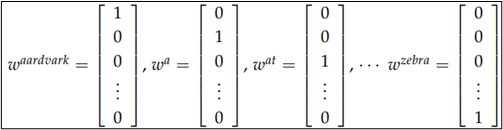
\includegraphics[width=13cm]{./img/word.png}
      \caption{ตัวอย่างของ Word Vector ของ คำว่า aardvark, a, at, zebra }\label{fig:word}
    \end{figure}
  \subsection{TF-IDF}
    \hspace{1cm} เป็นหนึ่งในวิธีหาความสำคัญของคำสำคัญในเอกสาร โดยพิจารณาจากค่าน้ำหนักของคำ แล้วนำมาประยุกต์ใช้กับการค้นคืนเอกสาร Information-retrieval 
    หรือ Text mining โดย TF-IDF มาจากผลคูณของสองค่านั้น คือ TF (Term Frequency) กับ IDF (Inverse Document Frequency) \cite{tfidf} 
    \[ TFIDF = TF * IDF \] 
    \hspace{1cm}โดย Term Frequency (TF) จะเป็นความถี่ของคำศัพท์ เพื่อหาว่าแต่ละคำนั้นปรากฏมากเท่าไหร่ในเอกสาร ยิ่งมีการใช้คำศัพท์ในเอกสารมากเท่าไหร่
    การพิจารณาว่าเอกสารนั้นมีเนี้ืหาเกี่ยวกับอะไรก็จะยิ่งมากขึ้นเท่านั้น ซึ่งค่า TF สามารถคำนวณได้จากสมการ \cite{tf} 

    \[ TF(word) = \frac{Number\ of\ this\ word\ in\ documant}{Number\ of\ words\ in\ document} \] 
    \hspace{1cm}ส่วน Inverse Document Frequency (IDF) เป็นการคำนวณค่าน้ำหนัก (Weight) ความสำคัญของแต่ละคำ โดยคำที่พบเจอได้บ่อยๆ (ในหลายๆเอกสาร) 
    จะมีค่า IDF ต่ำ ซึ่งบ่งบอกว่าคำเหล่านั้นจะไม่สามารถดึงเอาจุดเด่นของเอกสารที่คำเหล่านั้นปรากฏอยู่ออกมาได้ดี ซึ่งค่า IDF สามารถคำนวณได้จากสมการ \cite{tfidf} 

    \[ IDF(word) = \log\left[\frac{1 + n}{1 + DF(word)}\right]+1 \] 
    \hspace{1cm} โดยที่ n = จำนวนเอกสารทั้งหมดที่ใช้พิจารณา และ DF(word) = จำนวนเอกสารที่มีคำนั้นปรากฎอยู่
  \subsection{Random Forest}
    
    \begin{figure}[!ht]\centering
      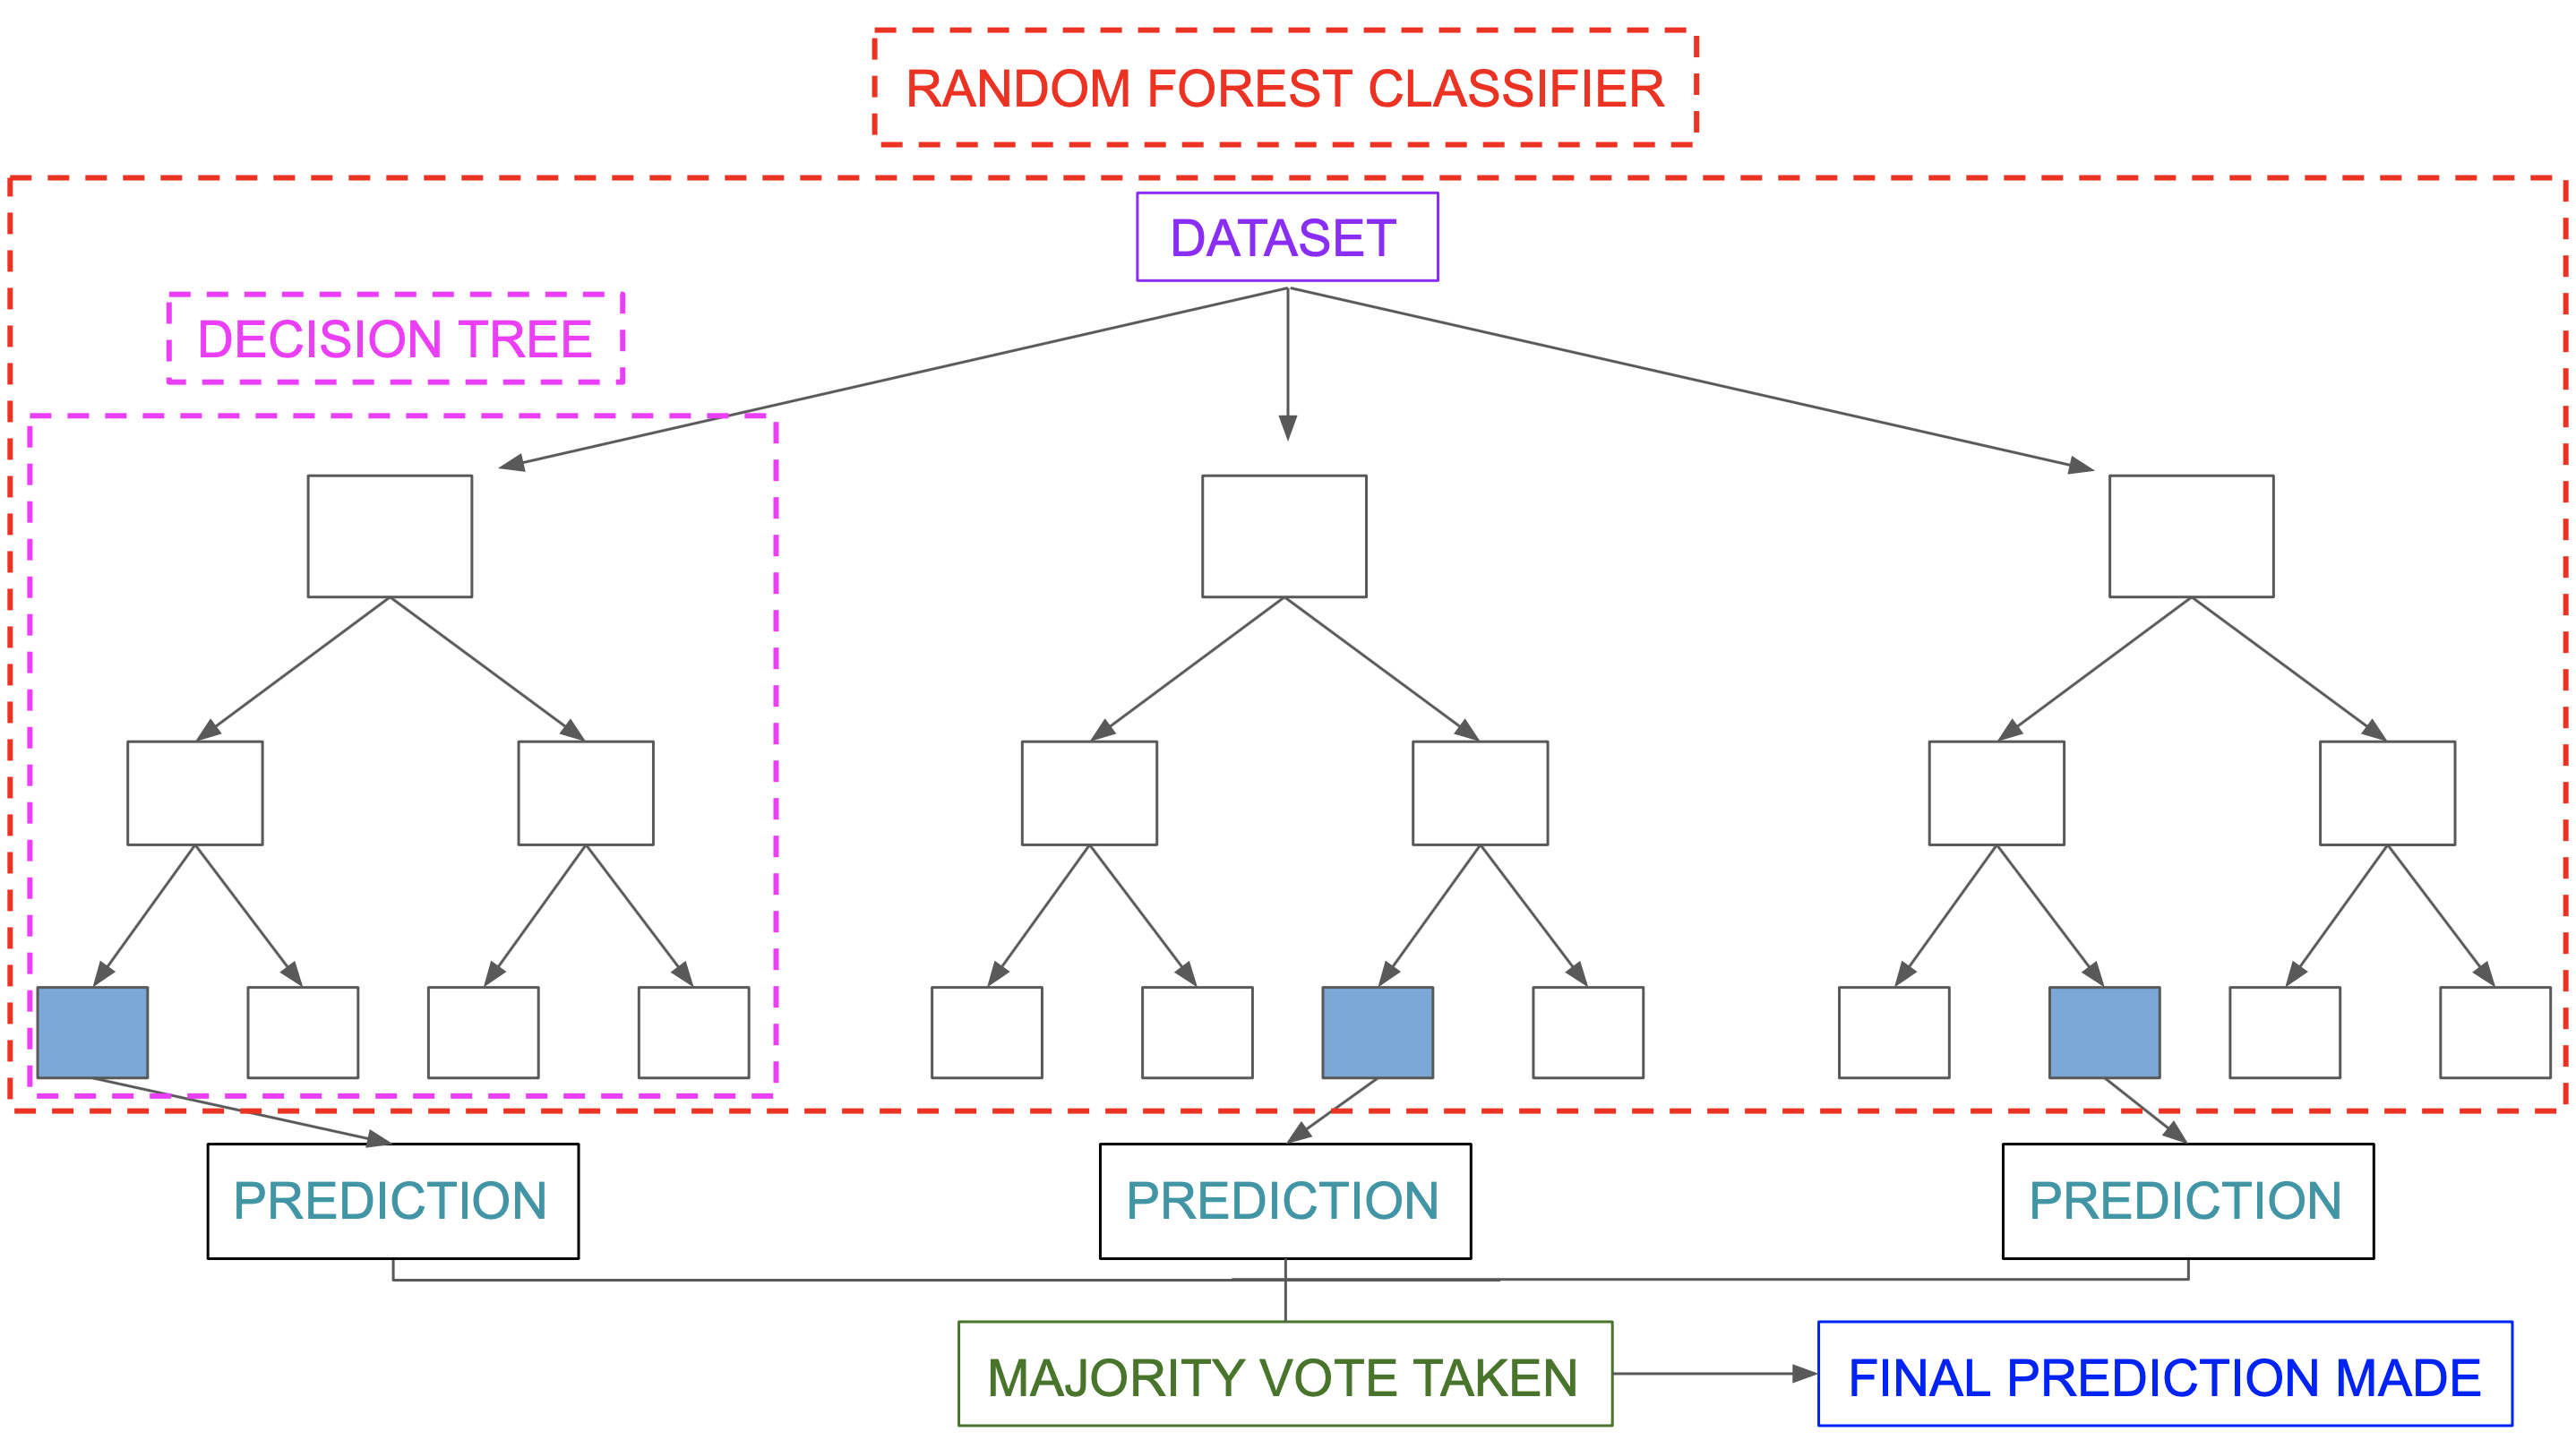
\includegraphics[width=13cm]{./img/tree.png}
      \caption{Random Forest}\label{fig:tree}
    \end{figure} 
    \hspace{1cm}คือขั้นตอนวิธีหนึ่งของ Machine Learning ที่นิยมใช้ทั้งกับปัญหาแบบ Regression และ Classification โดย Random Forest 
    เป็นขั้นตอนวิธีพัฒนาต่อยอดมาจาก Decision Tree ต่างกันที่ Random Forest เป็นการเพิ่มจำนวนต้นไม้เป็นหลายต้น ทำให้ประสิทธิภาพการทำงานและพยากรณ์สูงขึ้น 
    Random Forest มีหลักการทำงาน คือ จะแบ่งข้อมูลออกเป็น Decision Tree หลายต้น โดยแต่ละต้นจะได้รับ Feature และข้อมูลที่ไม่เหมือนกันทั้งหมด 
    เพื่อทำให้ได้ต้นไม้ที่มีความหลากหลายและมีความอิสระต่อกันมากขึ้น \cite{data_sci} 

    การทำงานของ Random Forest จะเริ่มต้นจาก 
    \begin{enumerate}
      \item ทำการสุ่มเลือก Feature และ Data จากชุดข้อมูลทั้งหมดที่มี 
      \item สร้าง Decision Tree จากชุดข้อมูลตัวอย่างแต่ละชุดและหาค่าพยากรณ์จากต้นไม้แต่ละต้น
      \item เลือกจำนวน Decision Tree ที่ต้องการ จากนั้นทำซ้ำในขั้นตอน 1 และ 2 ในการสร้างต้นไม้ 
      \item หาค่าพยากรณ์ โดยค่าพยากรณ์ที่ได้จะเป็นการให้ Decision Tree แต่ละต้นไม้หาค่าพยากรณ์ของใครของมัน จากนั้นค่าพยากรณ์สุดท้าย 
      ในกรณีที่ปัญหาเป็นเพื่อ Classification จะใช้วิธี Majority vote โดยค่าพยากรณ์ของ Decision Tree ต้นได้รับค่าผลโหวตมากที่สุดจะถูกเลือกให้เป็นค่าพยากรณ์ของปัญหา 
      แต่ถ้าเป็นปัญหา Regression จะใช้วิธีคำนวณหาค่าเฉลี่ย 
      โดยนำเอาค่าพยากรณ์ของทุก Decision Tree มาคำนวณหาค่าเฉลี่ย เพื่อแสดงเป็นค่าพยากรณ์ของปัญหา
    \end{enumerate}
  \subsection{K-Nearest Neighbor (KNN)}
    \hspace{1cm}มีหลักการทำงาน คือ จะใช้หลักการเปรียบเทียบความคล้ายคลึงกันของข้อมูลที่สนใจกับข้อมูลอื่นว่ามีความคล้ายคลึงหรืออยู่ใกล้กับข้อมูลใดมากที่สุด k ตัว 
    จากนั้นจะทำการตัดสินใจว่า คำตอบของข้อมูลที่สนใจนั้นควรเป็นคำตอบเดียวกับข้อมูลที่อยู่ใกล้ที่สุด k ตัวนั้น ทั้งนี้ k คือความถี่ของข้อมูลที่อยู่ใกล้กับข้อมูลที่สนใจ \cite{data_sci} 

    KNN มีขั้นตอนการทำงาน ดังนี้
    \begin{enumerate}
      \item ทำการกำหนดค่า k ซึ่งโดยทั่วไปจะกำหนดให้เป็นเลขคี่ เช่น 3, 5, 7 และ 9 เป็นต้น
      \item นำวัตถุที่ต้องการจำแนกมาวัดหาความคล้ายคลึงหรือความต่างกับข้อมูลทั้งหมดในชุดข้อมูล 
            โดยมาตรวัดระยะห่างที่นิยม ได้แก่ ระยะยูคลิด (Euclidean distance) ตามสมการ 

            \[ dist\left( p,q\right)   = \sqrt {\sum _{k=1}^{n}  \left( q_{k}-p_{k}\right)^2 }  \]
      \item เรียงลำดับวัตถุตามความคล้ายหรือความแตกต่าง จากคล้ายคลึงมากที่สุดไปหาน้อยที่สุด หรือจากแตกต่างน้อยที่สุดไปหามากที่สุด
      \item พิจารณาคำตอบจากจำนวนคลาสคำตอบที่มีมากที่สุดใน k ตัวที่มีความคล้ายมากที่สุด หรือมีความแตกต่างน้อยที่สุด
    \end{enumerate}
    \textbf{ยกตัวอย่าง} 
    \begin{figure}[!ht]\centering
      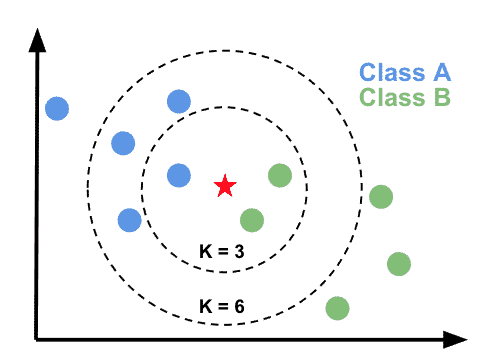
\includegraphics[width=7cm]{./img/knn.png}
      \caption{K-Nearest Neighbor}\label{fig:knn}
    \end{figure}

    \hspace{1cm}จากภาพข้างต้น ให้ข้อมูลที่สนใจคือดาวสีแดง วงกลมสีน้ำเงินคือ Class A และวงกลมสีเขียวคือ Class B ถ้าสนใจที่ค่า k เท่ากับ 3 
    จะได้ว่าข้อมูลที่สนใจจะมีความใกล้เคียงกับ Class B มากกว่า (สัดส่วนความใกล้เคียงของ Class A ต่อ Class B คือ 1:2) ดังนั้นคำตอบของข้อมูลที่สนใจก็จะเป็น Class B
    แต่ถ้าสนใจที่ค่า k เท่ากับ 6 ก็จะได้ว่าข้อมูลที่สนใจจะมีความใกล้เคียงกับ Class A มากกว่า (สัดส่วนความใกล้เคียงของ Class A ต่อ Class B คือ 2:1) ดังนั้นคำตอบของข้อมูลที่สนใจก็จะเป็น Class A 
  \subsection{Neural Network (NN)}

    \begin{figure}[!ht]\centering
      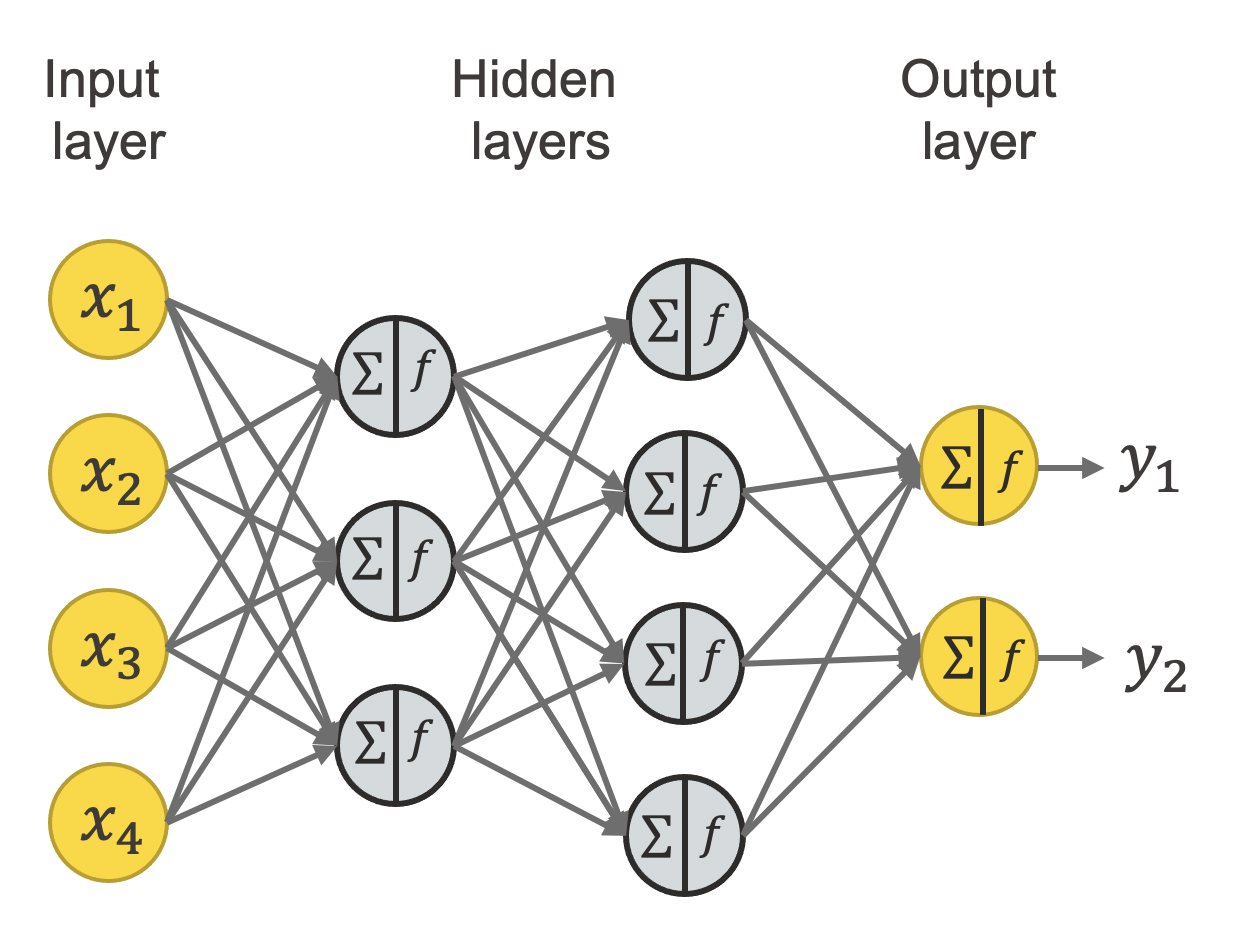
\includegraphics[width=7cm]{./img/nn.png}
      \caption{ส่วนประกอบของ Neural Network}\label{fig:nn}
    \end{figure}
    \hspace{1cm}โครงข่ายประสาทเทียม เป็นสาขาหนึ่งของปัญญาประดิษฐ์ Artificial Intelligence (AI) 
    เป็นแนวคิดที่ออกแบบระบบโครงข่ายคอมพิวเตอร์ให้เลียนแบบการทำงานของสมองมนุษย์ \cite{data_sci}

    ส่วนประกอบของ Neural Network ประกอบด้วย 3 ส่วน ได้แก่
    \begin{enumerate}
      \item Input Layer 
            
            \hspace{1cm}Layer นี้จะเป็นข้อมูล Input จำนวนของโหนดในชั้นนี้ขึ้นอยู่กับจำนวนของข้อมูล Input ว่า มีข้อมูลอะไรบ้างที่จะนำเข้ามาคิดใน Model เช่น ถ้าข้อมูลของลูกค้าเป็นข้อมูล Input ที่ประกอบด้วย 
            อายุ เพศ จังหวัดที่อาศัย รวมทั้งสิ้น 4 อย่าง ดังนั้นชั้นข้อมูล Input ก็จะมี 4 โหนด ซึ่งอาจจะเรียกปัจจัยที่นำมาวิเคราะห์เหล่านี้ว่าคุณลักษณะ (Feature)
      \item Hidden Layer 
            
            \hspace{1cm}Layer ที่อยู่ระหว่างกลาง ซึ่งจะมีผลอย่างมากต่อประสิทธิภาพในการเรียนรู้ของ Model ซึ่งใน Hidden Layer นั้นจะมีกี่ชั้นก็ได้ 
            และแต่ละชั้นจะมีจำนวนของ Nueral เท่าไหร่ก็ได้ ซึ่งการเพิ่มชั้นและจำนวน Neural จะส่งผลต่อการทำงานของ Model 
            ในส่วนของ Hidden Layer มีการทำงานเปรียบเสมือนส่วนที่เรียนรู้ข้อมูลเชิงลึก หรือ Deep Learning นั่นเอง โดยสิ่งสำคัญใน Hidden Layer อีกประการหนึ่งคือ 
            ทุก ๆ โหนดต้องประกอบด้วยฟังก์แบบไม่เป็นเชิงเส้น
      \item Output Layer 
            
            \hspace{1cm}Layer ที่จะนำเอาข้อมูลจากการคำนวณไปใช้และจำนวนของโหนดใน Layer นี้ขึ้นอยู่กับรูปแบบของข้อมูลออกที่จะเอาไปใช้ 
            ตัวอย่างเช่น ถ้างานที่ทำเป็นสมการถดถอย (Regression) ก็กำหนดให้ Output Layer เป็นแบบ 1 โหนด เพราะต้องการคำตอบเพียงค่าเดียว 
            ถ้าเป็นหลายค่าก็เพิ่มไปตามที่ต้องการ เช่น ในบางงานอาจจะทำนายหาตำแหน่งของภาพในแกน x และ y พร้อม ๆ กัน 
            ในกรณีนี้ก็ต้องกำหนดชั้นข้อมูลออกเป็น 2 โหนด เป็นต้น
    \end{enumerate}

    Neural Network ใช้กระบวนการเรียนรู้ข้อมูลโดยการปรับค่าน้ำหนักเป็นค่าที่เหมาะสมที่สุด 
    Neural Network มีการเรียนรู้ 2 แบบ คือ
    \begin{itemize}
      \item Supervised Learning เป็นการเรียนแบบที่มีการตรวจคำตอบ เพื่อให้ Neural Network ปรับตัว ชุดข้อมูลที่ใช้สอน Neural Network จะมีคำตอบไว้คอยตรวจดูว่า 
      Neural Network ให้คำตอบที่ถูกหรือไม่ ถ้าคำตอบไม่ถูก Neural Network ก็จะปรับตัวเองเพื่อให้ได้คำตอบที่ดีขึ้น 
      \item Unsupervised Learning เป็นการเรียนแบบไม่มีผู้แนะนำ ไม่มีการตรวจคำตอบว่าถูกหรือผิด Neural Network 
      จะจัดเรียงโครงสร้างด้วยตัวเองตามลักษณะของข้อมูลผลลัพธ์ที่ได้ Neural Network จะสามารถจัดหมวดหมู่ของข้อมูลได้
    \end{itemize}
    \hspace{1cm}กระบวนการเรียนรู้ของ Neural Network ถูกพัฒนาขึ้นหลากหลายวิธี เพื่อรองรับจุดประสงค์ในการใช้งานต่าง ๆ 
    วิธีการที่นิยมใช้มากที่สุดคือ Error correction และ Nearest neighbor

    \hspace{1cm}Error correction จะเป็น Back propagation ซึ่งมีการเรียนรู้ของ Model เกิดขึ้นเมื่อเอาค่าที่ได้จากการคำนวณในของ Forward Propagation 
    มาเทียบกับค่าของข้อมูลออกที่เกิดขึ้นจริง (Ground Truth) ค่าความผิดพลาดที่เกิดขึ้นเรียกว่า Cost Loss Error หรือ Residual

    \hspace{1cm}ดังนั้นกำหนดให้ข้อผิดพลาดของโหนด \(k\) (Error : \(e_k\)) สามารถคำนวณได้จากค่าความต่างของผลลัพธ์ (\(y\)) ของโหนด \(k\) 
    ในรอบที่ \(n\) แทนด้วยสัญลักษณ์ \(y_{k,n}\) และข้อมูล Output ที่เกิดขึ้นจริงของโหนด \(k\) แทนด้วยสัญลักษณ์ \(y^*_k\) ดังนั้นค่าความผิดพลาดคำนวณได้จากสมการ
    \[ e_k = y_{k,n} - y^*_k \] 

    \hspace{1cm}โดยค่าความผิดพลาด \(e_k\) ยิ่งมีค่าใกล้ศูนย์ยิ่งดี Back propagation ทำงานเหมือนสมองคน คือการเรียนรู้จากความผิดพลาด นั่นคือเมื่อรู้ค่าผิดพลาดของโหนด \(k\) แล้ว 
    จะนำค่าผิดพลาดนั้นมาคำนวณหาค่าน้ำหนักใหม่ (\(w_{new}\)) ในรอบที่ \(n+1\) ของโหนด \(k\) ดังสมการ
    \[ w_{new} = w_{old} - \lambda \frac{\partial E}{\partial w_{old}} \] 

    \hspace{1cm}โดย \(\lambda\) คือค่าคงที่ในการปรับน้ำหนักซึ่งอาจจะเรียกว่า Step หรือ Learning rate ซึ่งทุก ๆ รอบของการทำงาน จะมีการปรับค่าน้ำหนักใหม่ทุกครั้ง
    จนกว่าค่าน้ำหนักจะไม่เปลี่ยนแปลงหรือเปลี่ยนแปลงน้อย (Convergence) ถือเป็นค่าน้ำหนักที่เหมาะสมที่สุด (Optimization) จะมีผลทำให้การทำนายผลลัพธ์มีความแม่นยำมากยิ่งขึ้น
  \subsection{RESTful API}

    \begin{figure}[!ht]\centering
      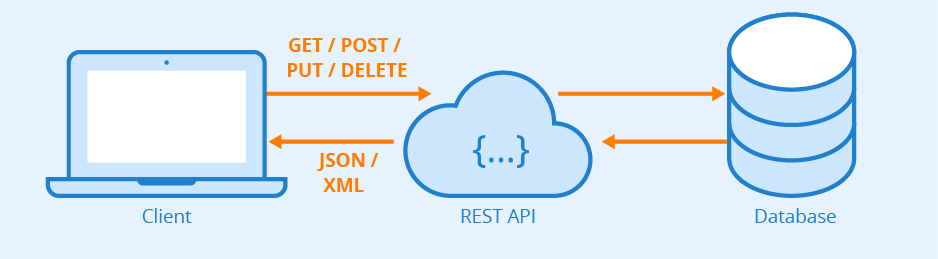
\includegraphics[width=13cm]{./img/rest.png}
      \caption{RESTful API}\label{fig:api}
    \end{figure}

    \hspace{1cm}เป็น Interface ที่ระบบคอมพิวเตอร์ 2 ระบบใช้เพื่อแลกเปลี่ยนข้อมูลผ่านอินเทอร์เน็ตได้อย่างปลอดภัย 
    แอปพลิเคชันส่วนใหญ่ต้องสื่อสารกับแอปพลิเคชันภายในอื่น ๆ และของบุคคลที่สามเพื่อทำงานต่าง ๆ ซึ่งจะอยู่บนมาตราฐานของโปรโตคอล HTTP \cite{api} 
    
    \hspace{1cm}ฟังก์ชันพื้นฐานของ RESTful API จะเหมือนกับการท่องอินเทอร์เน็ต ไคลเอ็นต์จะติดต่อกับเซิร์ฟเวอร์โดยใช้ API 
    เมื่อต้องใช้ทรัพยากร นักพัฒนา API อธิบายวิธีการที่ไคลเอ็นต์ควรใช้ REST API ในเอกสารประกอบ API ของแอปพลิเคชันเซิร์ฟเวอร์ 
    โดยการเรียกใช้ REST API มีขั้นตอนทั่วไปดังนี้
    \begin{itemize}
      \item ไคลเอ็นต์ส่งคำขอไปยังเซิร์ฟเวอร์ ไคลเอ็นต์ปฏิบัติตามเอกสารประกอบ API เพื่อจัดรูปแบบคำขอในลักษณะที่เซิร์ฟเวอร์เข้าใจได้
      \item เซิร์ฟเวอร์รับรองความถูกต้องของไคลเอ็นต์ และยืนยันว่าไคลเอ็นต์มีสิทธิ์ส่งคำขอดังกล่าว
      \item เซิร์ฟเวอร์รับคำขอและประมวลผลเป็นการภายใน
      \item เซิร์ฟเวอร์ส่งคืนการตอบสนองกลับไปยังไคลเอ็นต์ การตอบสนองมีข้อมูลที่บอกให้ลูกค้าทราบว่าคำขอดังกล่าวสำเร็จหรือไม่ การตอบสนองยังรวมถึงข้อมูลใดๆ ที่ไคลเอ็นต์ร้องขออีกด้วย
    \end{itemize}
    \hspace{1cm}นักพัฒนามักใช้ RESTful API โดยใช้เกณฑ์วิธีขนส่งข้อความหลายมิติ (Hypertext Transfer Protocol หรือ HTTP) 
    วิธีการ HTTP จะบอกให้เซิร์ฟเวอร์ทราบถึงสิ่งที่ต้องทำกับทรัพยากร โดยวิธีการ HTTP ทั่วไปมี 4 วิธีดังต่อไปนี้
    \begin{itemize}
      \item GET
            \newline เพื่อเข้าถึงทรัพยากรที่อยู่ที่ URL ที่ระบุบนเซิร์ฟเวอร์ ซึ่งสามารถแคชคำขอ GET และส่งพารามิเตอร์ในคำขอ RESTful API เพื่อสั่งให้เซิร์ฟเวอร์กรองข้อมูลก่อนส่ง
      \item POST
            \newline เพื่อส่งข้อมูลไปยังเซิร์ฟเวอร์ ซึ่งรวมถึงการแทนข้อมูลพร้อมกับคำขอ การส่งคำขอ POST เดียวกันหลายครั้งมีผลข้างเคียงเหมือนกับการสร้างทรัพยากรเดียวกันหลายครั้ง
      \item PUT
            \newline เพื่ออัปเดตทรัพยากรที่มีอยู่บนเซิร์ฟเวอร์ การส่งคำขอ PUT เดียวกันหลายครั้งในบริการเว็บ RESTful จะให้ผลลัพธ์เหมือนกัน ซึ่งแตกต่างจาก POST
      \item DELETE
            \newline เพื่อลบทรัพยากรออก โดยคำขอ DELETE สามารถเปลี่ยนสถานะเซิร์ฟเวอร์ได้ อย่างไรก็ตาม หากผู้ใช้ไม่มีการรับรองความถูกต้องที่เหมาะสม คำขอก็จะล้มเหลว
    \end{itemize}

  \subsection{Event Driven Architecture (EDA)}
    \hspace{1cm}เป็นแนวคิดที่ออกแบบระบบโครงข่ายคอมพิวเตอร์ให้สามารถตอบสนองต่อเหตุการณ์ที่เกิดขึ้นได้ โดยการส่งข้อมูลผ่านทางข้อความ ซึ่งเหตุการณ์ที่เกิดขึ้นนั้นจะถูกส่งไปยัง Event Handler
    และ Event Handler จะทำการประมวลผลเหตุการณ์นั้น ๆ ต่อไป \cite{eda} โดย Event Handler จะมีหน้าที่ดังนี้ 
    \begin{itemize}
      \item จัดการข้อมูลที่ได้รับจากเหตุการณ์ที่เกิดขึ้น
      \item ประมวลผลข้อมูลที่ได้รับจากเหตุการณ์ที่เกิดขึ้น
      \item ส่งข้อมูลไปยัง Event Handler อื่น ๆ ต่อไป
    \end{itemize}
  
  \subsection{Dependency Injection (DI)}
    \hspace{1cm}เป็น Design Pattern ที่ใช้ในการเขียนโปรแกรมเพื่อลดความผูกพันของโค้ด โดยการแยกส่วนของการสร้าง Object ออกจากการใช้งาน Object
    เพื่อให้การสร้าง Object นั้นสามารถนำไปใช้งานได้หลาย ๆ สถานการณ์ \cite{di} โดยการสร้าง Object จะมีคลาสที่เรียกว่า Container ซึ่งจะสร้าง Object และเก็บไว้ในตัวเอง
    ซึ่งเมื่อมีการเรียกใช้งาน Object จะทำการส่ง Object ที่ถูกสร้างไว้ให้กับคลาสที่ต้องการใช้งาน โดยไม่จำเป็นต้องสร้าง Object ใหม่ทุกครั้งที่มีการเรียกใช้งาน
    และสามารถนำ Object ไปใช้งานในสถานการณ์ต่าง ๆ ได้ จึงทำให้สามารถลดความผูกพันของโค้ดลงได้ ซึ่งจะทำให้ได้รับประโยชน์ ดังนี้
    \begin{itemize}
      \item ลดความซับซ้อนของโค้ด
      \item ลดความผูกพันระหว่างโค้ด
      \item ลดความซ้ำซ้อนของโค้ด
      \item ทำให้โค้ดมีความยืดหยุ่นมากขึ้น
      \item ทำให้การทดสอบโค้ดง่ายขึ้น
    \end{itemize}
  
  \subsection{Continuous Integration (CI)}
    \hspace{1cm}เป็นกระบวนการที่ใช้ในการพัฒนาซอฟต์แวร์ โดยจะทำการนำ Source Code ของเราผ่านกระบวนการ Testing, Building เพื่อให้ได้เป็นไฟล์ที่พร้อมใช้งานได้
    และเมื่อมีการเปลี่ยนแปลง Source Code จะทำการทดสอบและสร้างไฟล์ใหม่อัตโนมัติ \cite{ci_cd} ซึ่งจะทำให้ได้รับประโยชน์ดังนี้
    \begin{itemize}
      \item ลดเวลาในการทดสอบและการสร้างไฟล์
      \item ลดความผิดพลาดในการทดสอบ
      \item ลดความผิดพลาดในการสร้างไฟล์
      \item ลดเวลาในการแก้ไขข้อผิดพลาด
    \end{itemize}

  \subsection{Continuous Deployment (CD)}
    \hspace{1cm}เป็นกระบวนการที่ใช้ในการอัพเดทซอฟต์แวร์ โดยจะทำการนำไฟล์ที่พร้อมใช้งานไปอัพเดทใน Production โดยอัตโนมัติ \cite{ci_cd} ซึ่งจะทำให้ได้รับประโยชน์ดังนี้
    \begin{itemize}
      \item ลดเวลาในการอัพเดทซอฟต์แวร์
      \item ลดความผิดพลาดในการอัพเดทซอฟต์แวร์
      \item ลดเวลาในการแก้ไขข้อผิดพลาด
    \end{itemize}

  \subsection{Web Scraping}
    \hspace{1cm}Web Scraping \cite{agile} คือ การดึงข้อมูลจากหน้าเว็บไซต์ตามรูปแบบที่กำหนด เพื่อนำข้อมูลไปวิเคราะห์ตามจุดประสงค์ต่าง ๆ
    เป็นการดึงข้อมูลจาก Element หรือ Tag ของเว็บไซต์โดยเก็บเป็นรูปแบบต่าง ๆ ซึ่งเป็นวิธีการที่มีประโยชน์มากในกระบวนการรวบรวมข้อมูล (Data Collection)
    เนื่องจากแต่ละเว็บไซต์มีโครงสร้างที่ไม่เหมือนกัน ดังนั้นหากต้องการดึงข้อมูลจะต้องทำ Web Scraping ในการดึงข้อมูลตามโครงสร้างของเว็บไซต์นั้น ๆ 
    เพื่อให้ได้ข้อมูลในส่วนที่ต้องการ การทำ Web Scraping สามารถทำได้ด้วยการเขียนโค้ด หรือกรณีโครงสร้างเว็บไซต์ไม่ซับซ้อนสามารถใช้เครื่องมือช่วยทำ Web Scraping ได้
    ซึ่งในปริญญานิพนธ์นี้ได้ทำ Web Scraping ด้วยการเขียนโค้ด โดยใช้ Selenium และ BeautifulSoup เป็นเครื่องมือ
 
  \subsection{Agile}
    \hspace{1cm}Agile \cite{agile} หมายถึงหลักการและกระบวนการทํางานที่เน้นผลลัพธ์มากกว่าขั้นตอน 
    โดยการทํางานแบบ Agile นั้นเป็นการทํางานเป็นทีมโดยใช้วิธีการทํางานร่วมกัน 
    เพื่อให้ได้ผลลัพธ์ที่ต้องการตามเป้าหมายที่กําหนดไว้ การกําหนดเป้าหมายใน Agile จะเน้นการกําหนดเป้าหมายระยะสั้น ๆ 
    โดยแบ่งโครงการออกเป็นเฟสเล็ก ๆ หรือ Sprint ที่จะช่วยให้สามารถทํางานให้เสร็จสิ้นได้ในระยะเวลาอันสั้นๆ 
    โดย การทํางานแบบ Agile สามารถมีหลาย Sprint หรือโครงการได้ในเวลาเดียวกัน

    \hspace{1cm}ดังนั้นการนํา Agile มาใช้จะช่วยเพิ่มความคล่องตัวและความยืดหยุ่นในการพัฒนาโปรเจกต์หรืองาน 
    โดยทําให้สามารถปรับปรุงและปรับเปลี่ยนงานได้อย่างรวดเร็วตามความต้องการของลูกค้าหรือการเปลี่ยนแปลงในสภาพแวดล้อมได้ง่ายขึ้น 
    นอกจากนี้การทํางานแบบ Agile ยังช่วยสร้างทัศนคติที่ดีในการทํางานร่วมกันในทีม 
    โดยให้พนักงานได้รับการสนับสนุนและการแบ่งปันความรับผิดชอบในการทํางานร่วมกันอย่างเต็มที่ 
    ซึ่งจะช่วยเพิ่มประสิทธิภาพและคุณภาพของงานที่ทําให้สําเร็จได้ตามเป้าหมายที่กําหนดไว้มากขึ้น

\section{งานวิจัยที่เกี่ยวข้อง}
  \subsection{Machine learning approach to auto-tagging online content for content marketing efficiency:
    A comparative analysis between methods and content type}
    \hspace{1cm}ปัจจุบันนักการตลาดด้านเนื้อหาจะต้องประสบพบเจอกับเนื้อหาที่มีความซับซ้อนมากขึ้น 
    เนื่องจากเนื้อหาที่ไม่มีโครงสร้างที่ชัดเจนส่งผลให้การวิเคราะห์ การจัดการ และการจำแนกเนื้อหานั้นเป็นไปได้ยากยิ่งขึ้น 
    ดังนั้นจึงมีการเสนอวิธีการจำแนกหมวดหมู่ของเนื้อหาโดยอัตโนมัติ 
    โดยในงานวิจัยนี้ ผู้วิจัยได้ใช้ Machine Learning สำหรับการจัดหมวดหมู่ให้กับเนื้อหาทั้งหมด 3 โมเดลด้วยกัน ได้แก่
    Random Forest, K-Nearest Neighbor และ Neural Network 
    ซึ่งจากผลการวิจัย พบว่า Neural Network มีประสิทธิภาพมากที่สุด โดยได้ค่า F1 อยู่ที่ 70\%  
    สามารถจัดหมวดหมู่ให้กับ Online Content ที่ไม่มีหมวดหมู่ได้ถึง 99.6\% และสามารถจัดหมวดหมู่ให้กับ YouTube ที่ไม่มีหมวดหมู่ได้ถึง 96.1\% \cite{three_model}  

    \hspace{1cm}จากงานวิจัยนี้ทำให้ทราบถึงกระบวนการการทำ Auto-tagging Online Content ซึ่งคณะผู้จัดทำได้อิงกระบวนการบางส่วนตามงานวิจัยนี้
    เนื่องจากลักษณะงานที่มีความคล้ายกัน สิ่งที่คณะผู้จัดทำให้ความสนใจกับงานวิจัยนี้คือ การประเมิน Model การเตรียมข้อมูล และการใช้ Model หลากหลายรูปแบบ
    โดยงานวิจัยนี้ได้ใช้ค่า F1 Score ค่า Precision และค่า Recall สำหรับการประเมิน Model
    
    \hspace{1cm}ในส่วนของการเตรียมข้อมูล งานวิจัยนี้ได้มีการวิจัยใช้ลักษณะของบทความที่แตกต่างกัน เพื่อที่จะทราบว่าส่วนใดของบทความบ้างที่เหมาะสมกับการนำไปใช้งาน 
    โดยแบ่งลักษณะของบทความเป็นทั้งหมด 3 รูปแบบด้วยกัน ได้แก่ รูปแบบที่ 1 คือ มีเพียงหัวข้อ รูปแบบที่ 2 คือ มีหัวข้อและคำอธิบาย และรูปแบบที่ 3 คือ มีทั้งหัวข้อ คำอธิบาย และเนื้อหา
    ซึ่งจากผลการวิจัยพบว่า การใช้ส่วนของบทความทั้ง 3 ส่วน ได้แก่ หัวข้อ คำอธิบาย และเนื้อหา จะทำให้ได้ผลลัพธ์ของการทำ Auto-tagging ดีที่สุด 
    ดังนั้นคณะผู้จัดทำจึงเลือกที่จะใช้บทความทั้ง 3 ส่วนโดยอิงจากกงานวิจัย

    \begin{figure}[!ht]\centering
      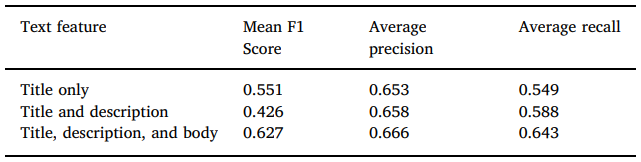
\includegraphics[width=13cm]{./img/text_feature.png}
      \caption{ผลการทดลองของงานวิจัยจากการใช้ Text Feature ที่แตกต่างกัน}\label{fig:feature}
    \end{figure}

    \hspace{1cm}นอกจากลักษณะของบทความ งานวิจัยนี้ได้มีการวิจัยใช้ Algorithm หลากหลายรูปแบบเพื่อเปลี่ยนคำให้เป็น Vector โดยวิจัยทั้งหมด 3 Algorithm ด้วยกัน
    ได้แก่ TF TF-IDF และ Doc2Vec ซึ่งจากผลการวิจัยพบว่า การใช้ TF-IDF จะทำให้ได้ผลลัพธ์ของการทำ Auto-tagging ดีที่สุด ดังนั้นคณะผู้จัดทำจึงเลือกที่จะใช้ TF-IDF
    สำหรับการแปลงคำเป็น Vector

    \begin{figure}[!ht]\centering
      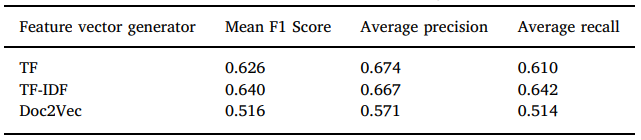
\includegraphics[width=13cm]{./img/vector.png}
      \caption{ผลการทดลองของงานวิจัยจากการใช้ Vector Generator ที่แตกต่างกัน}\label{fig:vector}
    \end{figure}

\section{ผลิตภัณฑ์ที่เกี่ยวข้อง}
  \subsection{Amazon Comprehend}
  \begin{figure}[!ht]\centering
  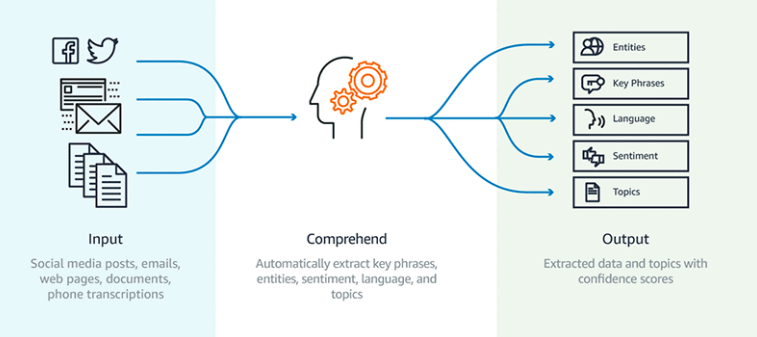
\includegraphics[width=13cm]{./img/aws.png}
  \caption{Amazon Comprehend}\label{fig:aws}
  \end{figure}
  \hspace{1cm}เป็นบริการ Natural Language Processing (NLP) ที่จะใช้ Machine Learning มาประมวลผลข้อมูลที่ไม่มีโครงสร้างเพื่อหาข้อมูลเชิงลึกที่มีคุณค่าจากข้อความในเอกสาร 
  สามารถลดความซับซ้อนของการทำงานการประมวลผลข้อมูลโดยการแยกข้อความ วลีสำคัญ หัวข้อ และอื่น ๆ จากเอกสารเพื่อการจัดเก็บข้อมูลอย่างเป็นระบบ
  ซึ่ง Amazon Comprehend ก็จะมีกรณีการใช้งานอยู่หลากหลายรูปแบบด้วยกัน \cite{aws} เช่น
  \begin{itemize}
    \item ตรวจจับความรู้สึกของลูกค้าและวิเคราะห์การโต้ตอบของลูกค้า และจัดหมวดหมู่คำขอการสนับสนุนขาเข้าโดยอัตโนมัติ สกัดข้อมูลเชิงลึกจากการสำรวจลูกค้าเพื่อปรับปรุงผลิตภัณฑ์
    \item ให้ความสำคัญกับบริบท โดยการทำให้เครื่องมือค้นหาสามารถจัดทำดัชนีวลี เอนทิตี และความรู้สึกที่สำคัญได้ ไม่ใช่แค่คำสำคัญเพียงอย่างเดียว
    \item ทำระบบอัตโนมัติให้กับการสกัดข้อมูลเชิงลึกจากกลุ่มข้อมูลของข้อสรุปทางกฎหมาย เช่น สัญญาและบันทึกของศาล ยกระดับการรักษาความปลอดภัยให้กับเอกสาร โดยการระบุและแก้ไขข้อมูลที่สามารถระบุตัวบุคคลได้ (PII)
    \item จำแนกและแยกเอนทิตีจากเอกสารบริการทางการเงิน เช่น การเรียกร้องค่าสินไหมทดแทนจากประกันภัย แพคเกจการจำนอง หรือหาความสัมพันธ์ระหว่างเหตุการณ์ทางการเงินในบทความเกี่ยวกับการเงิน 
  \end{itemize}
  \hspace{1cm}ถึงแม้ Amazon Comprehend จะเป็นบริการ Natural Language Processing (NLP) ที่จะใช้ Machine Learning คล้ายกับผลิตภัณฑ์ของเรา 
  แต่ก็มีข้อแตกต่างจากผลิตภัณฑ์ของเราตามตารางดังนี้ 
  \newpage
  \begin{longtable}[!ht]{lll}
    \caption{เปรียบเทียบผลิตภัณฑ์ระหว่าง Amazon Comprehend กับ AI-based Thai Content Tagging Platform}\label{tbl:aws} \\
    \hhline{===}
    \textbf{รายการ}     & \textbf{Amazon Comprehend}                                     & \textbf{AI-based Thai Content Tagging Platform} \\ \hline
    รองรับภาษาไทย        & ไม่รองรับภาษาไทย                                                 & รองรับภาษาไทย                                    \\ \hline
    ความง่ายในการใช้งาน    & 
    \begin{tabular}[c]{@{}l@{}}เหมาะสำหรับนักพัฒนา ผู้สร้างเนื้อหา \\ และนักการตลาด \end{tabular} & ผู้ใช้งานทั่วไปสามารถใช้ได้                            \\ \hline
    การนำไปประยุกต์ใช้งาน &
    \begin{tabular}[c]{@{}l@{}}ผู้ใช้สามารถประยุกต์ได้หลากหลาย   \\ แต่ต้องมีความเข้าใจในการพัฒนาโปรแกรม\end{tabular} &
    \begin{tabular}[c]{@{}l@{}}ฟังก์ชันการทำงานจำกัด   \\ โดยนักพัฒนาแพลตฟอร์ม\end{tabular}                                                  \\ \hhline{===}
  \end{longtable} 

\section{เทคนิคและเทคโนโลยีที่ใช้}
  \subsection{Development Tools}
    \begin{itemize}
      \item  JavaScript 
      
        \hspace{1cm}เป็นภาษาเขียนโปรแกรมที่ถูกพัฒนาและปฏิบัติตามข้อกำหนดมาตรฐานของ ECMAScript 
        เป็นภาษาระดับสูง คอมไพล์ในขณะที่โปรแกรมรัน (JIT) 
        และเป็นภาษาเขียนโปรแกรมแบบหลายกระบวนทัศน์ เช่น 
        การเขียนโปรแกรมเชิงขั้นตอน การเขียนโปรแกรมเชิงวัตถุ หรือการเขียนโปรแกรมแบบ Functional 
        ภาษา JavaScript มีไวยากรณ์ที่เหมือนกับภาษา C ใช้วงเล็บเพื่อกำหนดบล็อคของคำสั่ง 
        นอกจากนี้ JavaScript ยังเป็นภาษาที่มีประเภทข้อมูลแบบ Dynamic 
        เป็นภาษาแบบ Prototype-based และ First-class Function  \cite{js} 
        
        \hspace{1cm}เป็นภาษาโปรแกรมที่นักพัฒนาใช้ในการสร้างหน้าเว็บแบบ Interactive 
        ทำให้เว็บไซต์สามารถตอบสนองกับผู้ใช้งาน 
        ทั้งมี Library ที่ช่วยให้การพัฒนาเว็บไซต์ได้ง่ายขึ้นจำนวนมาก 
        จึงเป็นภาษาที่นิยมในการเขียนเว็บไซต์
      \item Java
      
        \hspace{1cm}เป็นภาษาเขียนโปรแกรมที่ได้รับความนิยมเป็นอย่างมาก มีการใช้งานอย่างกว้างขวาง เป็นจากมีประสิทธิภาพการทำงานสูง และสามารถรันได้ในทุก Platform 
        โดยไม่ต้องทำการ Compile Code ใหม่ผ่าน JVM (Java Virtual Machine) เนื่องด้วยเป็นภาษาที่มีการพัฒนาต่อเนื่องมาอย่างยาวนาน 
        จึงทำให้มี Library ให้เลือกใช้งานมากมาย โดยรูปแบบการเขียนโปรแกรมภาษา Java จะเขียนโดยใช้หลักการ OOP (Object Oriented Programming) \cite{java}
      \item  Golang
      
      \hspace{1cm}เป็นภาษาเขียนโปรแกรมแบบ Open Source ที่ถูกพัฒนาขึ้นโดยบริษัท Google ในปี 2007 
      และได้รับความนิยมเพิ่มขึ้นมากขึ้นเรื่อย ๆ ในยุคนี้ \cite{go} เนื่องจากประสิทธิภาพในการทำงานที่สูงและใช้ทรัพยากรในการทำงานต่ำ 
      อีกทั้งยังมี Garbage Collector ในการช่วยจัดการกับ Memory 
      นอกจากประสิทธิภาพแล้ว ความง่ายในการเรียนรู้ของภาษา Golang 
      ยังสามารถทำความเข้าใจได้ง่าย ทำให้เป็นภาษาที่ได้รับความนิยมในวงกว้าง 
      
      \hspace{1cm}Golang เป็นภาษาที่เหมาะสำหรับการทำ Web Development มาก เนื่องจากสามารถใช้สร้างระบบที่รองรับการทำงานใน Scale ใหญ่ที่มี Request จำนวนมากได้ 
      ซึ่ง Golang ถูกออกแบบมาเพื่องานประเภทนี้โดยเฉพาะ ยกตัวอย่างเช่น มี HTTP Package อยู่ใน Standard Library ของ Go โดยที่ไม่ต้องลง Library เพิ่มเติม 
      หรือจะใช้ Framework ต่าง ๆ ช่วยให้ทำ Web Development ได้ง่ายและสะดวกขึ้น \cite{go}
      \item  Python
      
      \hspace{1cm}เป็นภาษาเขียนโปรแกรมที่ใช้อย่างแพร่หลายในเว็บแอปพลิเคชัน การพัฒนาซอฟต์แวร์ วิทยาศาสตร์ข้อมูล และ แมชชีนเลิร์นนิง (ML)
      นักพัฒนาใช้ Python เนื่องจากมีประสิทธิภาพ เรียนรู้ง่าย และสามารถทำงานบนแพลตฟอร์มต่างๆ ได้มากมาย ทั้งนี้ซอฟต์แวร์ Python สามารถดาวน์โหลดได้ฟรี 
      ผสานการทำงานร่วมกับระบบทุกประเภท และเพิ่มความเร็วในการพัฒนา 
      ภาษา Python มีกรณีการใช้งานหลายอย่างในการพัฒนาแอปพลิเคชัน ซึ่งรวมถึงตัวอย่างดังต่อไปนี้ \cite{python}
      \begin{itemize}
        \item การพัฒนาเว็บฝั่งเซิร์ฟเวอร์
        
        \hspace{1cm}การพัฒนาเว็บฝั่งเซิร์ฟเวอร์ประกอบด้วยฟังก์ชัน Backend ที่ซับซ้อน ซึ่งเว็บไซต์ดำเนินการเพื่อแสดงข้อมูลต่อผู้ใช้ 
        ตัวอย่างเช่น เว็บไซต์ต้องโต้ตอบกับฐานข้อมูล สื่อสารกับเว็บไซต์อื่น และปกป้องข้อมูลเมื่อส่งข้อมูลผ่านเครือข่าย 
        
        \hspace{1cm}Python มีประโยชน์สำหรับการเขียนโค้ดฝั่งเซิร์ฟเวอร์ เนื่องจากมี Library จำนวนมากที่ประกอบด้วยโค้ดที่เขียนไว้ล่วงหน้าสำหรับฟังก์ชัน Backend ที่ซับซ้อน 
        นักพัฒนายังใช้ Framework Python ที่หลากหลายซึ่งมีเครื่องมือที่จำเป็นทั้งหมด เพื่อสร้างเว็บแอปพลิเคชันได้เร็วขึ้นและง่ายขึ้นอีกด้วย ตัวอย่างเช่น นักพัฒนาสามารถสร้างโครงสร้างเว็บแอปพลิเคชันได้ภายในไม่กี่วินาที 
        เนื่องจากไม่จำเป็นต้องเขียนขึ้นใหม่ทั้งหมด จากนั้นนักพัฒนาสามารถทดสอบได้โดยใช้เครื่องมือทดสอบของ Framework โดยไม่ต้องพึ่งพาเครื่องมือทดสอบภายนอก
        \item วิทยาศาสตร์ข้อมูลและแมชชีนเลิร์นนิง (ML)
        
        \hspace{1cm}วิทยาศาสตร์ข้อมูลดึงความรู้อันมีคุณค่าจากข้อมูลและแมชชีนเลิร์นนิง (ML) จะสอนคอมพิวเตอร์ให้เรียนรู้จากข้อมูลโดยอัตโนมัติและทำนายได้อย่างแม่นยำ 
        นักวิทยาศาสตร์ข้อมูลใช้ Python สำหรับงานด้านวิทยาศาสตร์ข้อมูลต่าง ๆ ดังต่อไปนี้
          \begin{itemize}
            \item การแก้ไขและลบข้อมูลที่ไม่ถูกต้อง ซึ่งเรียกว่าการทำความสะอาดข้อมูล
            \item การแยกและเลือกคุณสมบัติต่าง ๆ ของข้อมูล
            \item การระบุประเภทข้อมูล ซึ่งเป็นการเพิ่มชื่อที่มีความหมายสำหรับข้อมูล
            \item การค้นหาสถิติต่าง ๆ จากข้อมูล
            \item การแสดงข้อมูลด้วยภาพโดยใช้แผนภูมิและกราฟ เช่น แผนภูมิเส้น กราฟแท่ง ฮิสโทแกรม และแผนภูมิวงกลม
          \end{itemize}
        \hspace{1cm}นักวิทยาศาสตร์ข้อมูลใช้ไลบรารี Python ML เพื่อฝึกฝนโมเดล ML และสร้างตัวจำแนกที่จำแนกประเภทข้อมูลได้อย่างแม่นยำ 
        บุคคลในแวดวงต่าง ๆ ใช้ตัวจำแนกแบบ Python เพื่อทำงานด้านการจำแนกประเภท เช่น การจำแนกประเภทรูปภาพ ข้อความ 
        และการรับส่งข้อมูลทางเครือข่าย การรู้จำเสียง และการจดจำใบหน้า นักวิทยาศาสตร์ข้อมูลยังใช้ Python สำหรับ Deep Learning ซึ่งเป็นเทคนิค ML ขั้นสูง
        \item การพัฒนาซอฟต์แวร์
        
        \hspace{1cm}นักพัฒนาซอฟต์แวร์มักใช้ Python สำหรับงานด้านการพัฒนาและการประยุกต์ใช้ซอฟต์แวร์ต่าง ๆ ดังนี้
          \begin{itemize}
            \item การติดตามบักในโค้ดของซอฟต์แวร์
            \item การสร้างซอฟต์แวร์โดยอัตโนมัติ
            \item การดูแลการจัดการโครงการด้วยซอฟต์แวร์
            \item การพัฒนาต้นแบบซอฟต์แวร์
            \item การพัฒนาแอปพลิเคชันบนเดสก์ท็อปโดยใช้ Library ส่วนติดต่อผู้ใช้แบบกราฟิก (Graphical User Interface หรือ GUI)
            \item การพัฒนาเกมที่ใช้ข้อความแบบง่ายๆ ไปจนถึงวิดีโอเกมที่ซับซ้อนมากขึ้น
          \end{itemize}
      \end{itemize}
      \item Google Colaboratory
      
      \hspace{1cm}เป็นบริการ Cloud อีกหนึ่งบริการจาก Google Research เป็น IDE ที่อนุญาตให้ผู้ใช้เขียน Source code ในตัวแก้ไขและเรียกใช้จากเบราว์เซอร์ 
      รองรับภาษาเขียนโปรแกรม Python และเน้นงานแมชชีนเลิร์นนิง การวิเคราะห์ข้อมูล เป็นต้น 
      Google Colaboratory เป็นบริการ Software as a Service (Saas) โฮสต์โปรแกรม Jupyter Notebook บน Cloud จาก Google ซึ่งฟังก์ชั่นที่โดดเด่น ดังนี้ \cite{colab}
        \begin{itemize}
          \item แก้ไขและเรียกใช้โค้ดใน Python
          \item จัดเก็บงานใน Google Drive เพื่อไม่ให้สูญหาย
          \item แบ่งปัน Notebook กับผู้อื่นได้ (ข้อความ โค๊ด ผลลัพธ์ และความคิดเห็น)
          \item นำเข้า Jupyter Notebook หรือ IPython ได้
          \item ดาวน์โหลด Colab Notebook ในเครื่องจาก Google Drive ได้
        \end{itemize}
      \item Figma
      
      \hspace{1cm}เป็นเครื่องมือสำหรับใช้ออกแบบตั้งแต่เว็บไซต์, แอปพลิเคชัน สำหรับ UX/ UI Designer ทั่วโลก 
      หรือใช้สำหรับการแบบโลโก้, artwork ต่าง ๆ ของสายงาน Graphic Design รวมไปถึงคนทั่วไปที่ใช้ในการออกแบบ Presentation 
      Figma ให้ความสำคัญในเรื่องของการทำงานร่วมกันภายในทีม ทำให้ทีม UX/ UI Design ทำงานกันได้สะดวกมากขึ้น 
      รวมไปถึงส่งเสริมการทำระหว่างทีมที่ช่วยให้ Designer ส่งต่องานกับ Developer ได้ง่ายมากยิ่งขึ้น 
      ซึ่ง Figma จะใช้งานในรูปแบบ browser-based ที่ทุกคนสามารถทำงานพร้อมกันได้ 
      และมี Features ที่ช่วยให้การส่งต่องานระหว่างทีมทำได้ง่ายขึ้นกว่าเครื่องมือการออกแบบอื่น ๆ 
      โดยแบ่ง Feature การทำงานเป็น 4 ด้านดังนี้ \cite{figma}
        \begin{itemize}
          \item Collaboration Features
          \newline สามารถใช้งานพร้อมกันได้แบบ real-time บนเว็บ โดยไม่ต้องติดตั้งโปรแกรมในเครื่อง และไม่ต้องกด save แม้แต่ครั้งเดียว
          \item Design Features
          \newline มีฟีเจอร์ด้านงานออกแบบ ตั้งแต่เริ่มต้นออกแบบจนถึงส่งงานต่อให้ Developer
          \item Prototyping Features
          \item Design systems features
        \end{itemize}
    \end{itemize}
  \subsection{Database Tools}
    \begin{itemize}
      \item PostgreSQL
      
      \hspace{1cm}เป็น Open Source Object-Relational Database ที่ใช้งานกันอย่างแพร่หลาย มีการพัฒนาให้สามารถรองรับข้อมูลเพิ่มเติมได้
      หลายประเภท เช่น UUID, Array, JSON ทำให้สามารถนำไปประยุุกต์ใช้ได้หลากหลาย เป็นระบบฐานข้อมูล SQL (Structure Query Language)
      เช่นเดียวกับ MySQL  \cite{postgresql}
    \end{itemize}
  \subsection{DevOps Tool}
    \begin{itemize}
      \item Git
      
      \hspace{1cm}ระบบจัดการแก้ไข (Version Control System) ติดตามการเปลี่ยนแปลงของไฟล์ต่าง ๆ ในโปรเจค ช่วยทำให้สามารถทำงานอย่างเป็นระบบ 
      สามารถติดตาม ตรวจสอบ การพัฒนา ดูประวัติการเปลี่ยนแปลงของไฟล์ต่าง ๆ เพื่อดูการเปลี่ยนแปลงเผื่อเกิดปัญหาก็สามารถย้อนกลับได้ \cite{git}

      \item Github
      
      \hspace{1cm}เว็บไซต์ที่ให้บริการ Git (Version Control Repository) โดยให้บริการบนออนไลน์แพลตฟอร์ม 
      ที่จะมีฟีเจอร์ที่จะช่วยให้นักพัฒนาคนอื่น ๆ สามารถมีส่วนร่วมในการทำงานแก้ไขโค้ดที่อยู่ใน Repository ได้
      ซึ่งสามารถตั้งค่า Repository เป็น Public ให้ทุกคนสามารถเข้าถึงได้ หรือ Private เพื่อใช้งานเฉพาะกลุ่มได้ \cite{github}

      \item Docker
      
      \hspace{1cm}แพลตฟอร์มซอฟต์แวร์ที่ช่วยให้นักพัฒนาซอฟต์แวร์สามารถสร้าง ทดสอบ และติดตั้งแอปพลิเคชันผ่านมาตราฐานของคอนเทนเนอร์ซึ่งจะ
      ช่วยในการจัดการสภาวะแวดล้อมของระบบ โค้ด และรันไทม์ ซึ่งเมื่อใช้ Docker จะช่วยให้สามารถติดตั้งแอปพลิเคชันให้เหมาะกับทุกสภาวะแวดล้อมได้อย่างรวดเร็ว \cite{docker} 
    \end{itemize}
  
  \subsection{Library Tools}
    \begin{itemize}
      % \item Gin
      
      % \hspace{1cm}เป็น Golang Web Framework ยอดนิยมในการพัฒนาระบบ Web Backend ช่วยให้สามารถจัดการกับ Routing, Middleware, และอื่น ๆ ที่เกี่ยวกับพัฒนาระบบเบื้องหลัง ให้มีความง่ายมากยิ่งขึ้น
      %  อีกทั้งยังมีการทำงานที่รวดเร็ว และใช้ทรัพยากรในการทำงานน้อย \cite{gin}

      % \item Gorm
      
      % \hspace{1cm}เป็น Golang ORM (Object Relational Mapping) ช่วยให้เราสามารถ Map ระหว่างโครงสร้างของ Column ใน Table ของ Database
      % ของ Field ของ Struct ในภาษา Golang ได้ ซึ่งจะทำให้ช่วยลดการ redundant, duplicate ของโค้ด \cite{gorm}

      \item Vue
      
      \hspace{1cm}เป็น JS Library ที่รวมเอาข้อดีของ Angular กับ React มารวมกัน มีการประมวลผลที่รวดเร็ว \cite{vue1}
      โดยเป็น "Progressive Framework"" สำหรับสร้าง User Interface (UI) ซึ่ง Progressive คือการที่ Vue.js ใช้เป็นเหมือนส่วนเพิ่มความสามารถที่เอาไปใช้งานกับ HTML 
      ซึ่ง Library นี้จะจัดการในส่วนของ View เท่านั้น เพื่อให้สามารถนำ Vue ไปใช้งานร่วมกับ Library อื่น ๆ ได้สะดวก 
      และเหมาะสำหรับการทำ Single-Page Applications (SPA) หรือเว็บที่ไม่ต้องเปลี่ยนหน้าบ่อย \cite{vue2}

      \item Nuxt.js
      
      \hspace{1cm}เป็น Javascript Framework ที่พัฒนาต่อยอดมาจาก Vue.js ซึ่งเป็นเครื่องมือที่ช่วยให้การพัฒนาและการแสดงผลบนเว็บแอปพลิเคชัน 
      มีความสะดวกสบาย สามารถพัฒนาต่อยอดผลงานได้อย่างมีประสิทธิภาพ \cite{nuxt}
       
      \item Pandas
      
      \hspace{1cm}เป็น Library Python แบบ Open Source ที่มีเครื่องมือจัดการและวิเคราะห์ข้อมูลประสิทธิภาพสูง
      โดยใช้โครงสร้างข้อมูลที่ชื่อ Pandas มาจากคำว่า Panel Data (ชุดข้อมูลหลายมิติ) มีจุดเด่นด้านการวิเคราะห์ข้อมูล (Data Analysis) 
      และการทำความสะอาด (Data Cleaning) ซึ่งเป็น Process ที่สำคัญมากในการทำงานกับข้อมูล โดยมี Feature การทำงานดังนี้ \cite{pandas}
        \begin{itemize}
          \item Object DataFrame ที่รวดเร็วและมีประสิทธิภาพ พร้อมการสร้าง Index เริ่มต้นและ Index ที่กำหนดเองได้
          \item เป็นเครื่องมือสำหรับโหลดข้อมูลลงใน In-memory Data Objects จากสกุลไฟล์ต่าง ๆ
          \item การจัดตำแหน่งข้อมูลและจัดการข้อมูลที่ขาดหายไป
          \item Reshaping และ Pivoting data
          \item การทำ label สำหรับการ Slicing, การ Indexing และ Subsetting ชุดข้อมูลที่มีขนาดใหญ่
          \item โครงสร้างข้อมูลสามารถ Delete หรือ Insert ได้
          \item จัดกลุ่มตาม Engine เพื่อให้สามารถใช้การดำเนินการ Split-Apply-Combine กับ Data Set
          \item การ Merging และ Joining ของ Data Set ที่มีประสิทธิภาพสูง
          \item การสร้าง Range ของวันและความถี่ของการเปลี่ยนแปลง การย้าย Window Statistics การย้าย Window Linear Regressions การ Shift วัน และการ Lagging
        \end{itemize}
        
      \item NumPy
      
      \hspace{1cm}เป็น Library ที่ใช้ในการคำนวนทางคณิตศาสตร์ในภาษา Python \cite{numpy} ซึ่งภายในถูกเขียนด้วยภาษา C จึงทำงานได้เร็วและมีประสิทธิภาพ 
      โดย NumPy มีความสามารถในการจัดการกับอาเรย์หลายมิติและข้อมูลแบบเมทริกซ์
      
      \item Natural Language Toolkit
      
      \hspace{1cm}หรือเรียกว่า NLTK เป็น Library สำหรับการประมวลผลภาษาธรรมชาติ (NLP) ของภาษาอังกฤษ โดยเขียนในภาษา Python 
      พัฒนาขึ้นโดย Steven Bird และ Edward Lope NLTK มีฟังก์ชันสำหรับการแบ่งประเภท ตัดคำ กำกับไวยากรณ์ประโยค และอื่น ๆ
      
      \item SpaCy
      
      \hspace{1cm}เป็น Library Open Source สำหรับการประมวลผลภาษาธรรมชาติขั้นสูง (NLP) 
      ที่เขียนด้วยภาษา Python พร้อมด้วยองค์ประกอบใน Cython (ส่วนต่อขยาย C ของ Python ออกแบบมาเพื่อให้ C มีประสิทธิภาพเข้ากับโปรแกรม python) 
      จึงเป็น Library ที่ค่อนข้างเร็ว ซึ่ง SpaCy ให้ API ในการเข้าถึงวิธีการและคุณสมบัติที่สามารถควบคุม โดยการสร้างแบบจำลองการเรียนรู้ของเครื่อง (Machine Learning) และ Deep Learning
      นอกจากนี้ SpaCy ยังสามารถทำงานร่วมกับ Library อื่นได้ เช่น NLTK
      
      \hspace{1cm}SpaCy ถูกออกแบบสำหรับการใช้งานและช่วยสร้างแอปพลิเคชันที่ประมวลผลและเข้าใจข้อความจำนวนมาก 
      สามารถใช้ในการสร้างการดึงข้อมูลหรือระบบความเข้าใจภาษาธรรมชาติหรือข้อความก่อนการประมวลผลสำหรับ Deep Learning 
      คุณสมบัติบางอย่าง SpaCy มีให้ ได้แก่ การแบ่งคำ (Tokenization) การติดแท็กส่วนของคำพูด (Part-of-Speech Tagging)
      การจำแนกข้อความ (Sentence Boundary Detection) และการจดจำเอนทิตีที่มีชื่อ (Named Entity Recognition) \cite{spacy}
      
      \item Scikit-learn
      
      \hspace{1cm}เป็น Library ในการทำ Machine Learning ที่ควรศึกษาเอาไว้ เนื่องจากมีความง่ายและมีประสิทธิภาพในการทำ Predictive Data Analysis 
      เช่น Support Vector Machines(SVMs) Random Forests Gradient Boosting K-means และ DBSCAN 
      ซึ่งจะใช้อัลกอริทึมเหล่านี้เมื่อเราสร้างและฝึก Model สำหรับทำ Machine Learning \cite{pylib}
      
      \item Keras
      
      \hspace{1cm}เป็น Deep Learning Library ที่ได้รับความนิยมอย่างรวดเร็ว เนื่องจากใช้งานง่ายแต่มีประสิทธิภาพสูงในการรัน Model 
      ซึ่ง Backend ของ Keras มีทั้ง Tensorflow และ Theano ซึ่งจัดเป็น Deep Learning Library ที่มีสมรรถนะสูงทั้งคู่
      Keras สามารถใช้เพิ่อทำงานประเภท Regression Classification หรือประมวลผลรูปภาพได้ \cite{pylib}
      
      \item Tensorflow
      
      \hspace{1cm}เป็น Library สำหรับสร้าง Machine Learning Models แบบ Open Source จาก Google สามารถใช้งานได้ดีกับภาษา Python 
      แต่ก็ใช้งานร่วมกับภาษาอื่นๆ เช่น C, Java หรือ Go ได้เช่นกัน และยังมี Community ขนาดใหญ่ ทำให้สามารถค้นหาข้อมูลหรือสอบถามเวลาเจอปัญหาได้ง่าย \cite{pylib}

      \item BeautifulSoup

        \hspace{1cm}เป็น Library สำหรับทำ Web scraping หรือการดึงข้อมูลผ่านทางหน้าเว็บไซต์ ซึ่งหลังจากดึงข้อมูลเสร็จ จะเข้าสู่กระบวนการสกัด (Extract) 
        เอาเฉพาะข้อมูลที่ต้องการ เพื่อนำมาเก็บไว้ในรูปแบบที่ต้องการเป็นแหล่ง Data Source เพื่อใช้งานต่อไป โดยจะใช้ภาษา Python ในการเขียน Script \cite{beautifulsoup}

      \item Selenium 
      
        \hspace{1cm}เป็นเครื่องมือที่ช่วยให้สร้างโปรแกรมสำหรับการทดสอบเว็บไซต์ \cite{selenium} โดยจะสร้าง Web Browser จำลองขึ้นมาโดยใช้การเขียนโปรแกรมในภาษาต่าง ๆ
        เช่น Java Python หรือ Javascript ติดต่อกับไลบารีของ WebDriver เพื่อเข้าถึงคอนโทรลที่แสดงผ่าน Web Browser ได้
        แล้วทำการควบคุมให้คลิกแบบอัตโนมัติ ควบคุมปรับเปลี่ยนตัวเลือกหรือใส่ค่าต่าง ๆ ที่จำเป็นแบบอัตโนมัติ 
        รวมถึงสามารถแก้ไข Code HTML บางส่วนให้เป็นไปตามที่ต้องการเพื่อทดสอบการแสดงผลของเว็บไซต์ได้
        นอกจากนี้การใช้ Selenium เพื่อสร้าง Web Browser จำลองยังสามารถนำมาใช้ร่วมกับการดึงข้อมูลจากหน้าเว็บไซต์ เพื่อใช้ข้อมูลจากเว็บไซต์นั้น ๆ ได้
    \end{itemize}
  \subsection{Infrastructure Tools}
    \begin{itemize}
      \item Google Cloud Platform (GCP)
      
      \hspace{1cm}เป็นบริการ Cloud ที่ให้บริการโดยบริษัท Google ซึ่งมีบริการที่ช่วยส่งเสริมการพัฒนาแอปพลิเคชันให้มีความสะดวกสบายมากยิ่งขึ้น 
      ช่วยให้ลดค่าใช้จ่ายในการลงทุน Server หรือ Hardware ต่าง ๆ ที่ใช้ในการรันแอปพลิเคชัน และมีผู้ดูแลระบบให้ตลอด 24 ชม. อีกทั้งในบางบริการยังมีการคิดเงินแบบ Pay as you go 
      หมายถึงเราจะจ่ายเงินเฉพาะสิ่งที่เราใช้จริง ๆ เท่านั้น ไม่คิดค่าใช้จ่ายขณะที่เราไม่ได้ใช้งาน ซึ่ง Google มีจุดเชื่อมต่อ Network อยู่ทั่วโลกมากกว่า 33 ประเทศ และมีบริการให้เลือกใช้งานมากมาย \cite{gcp}

      \item Cloud Pub/Sub
      
      \hspace{1cm}บริการรับส่งข้อมูลระหว่าง Service เป็น Managed Service ที่ให้บริการโดย GCP จะมีแบ่งเป็น 3 ส่วนหลัก ๆ 
      คือ Publisher คือผู้ส่งข้อมูลโดยจะมีการ กำหนด topic เพื่อให้ Subscriber หรือผู้รับ รอรับข้อมูลจาก topic นั้น ๆ 
      โดยจะมี Cloud Pub/Sub เป็นสื่อการในการสื่อสารระหว่าง Publisher กับ Subscriber ซึ่งจะเป็นการสื่อสารแบบ asynchronously \cite{pubsub} 
      ซึ่งการนำ Cloud Pub/Sub มาใช้งานยังมีข้อดีอื่น ๆ อีกเช่น
      \begin{itemize}
        \item ไม่ต้องติดตั้ง หรือดูแลเนื่องจากเป็นบริการให้บริการโดย Google สามารถใช้งานได้ทันที
        \item มีความเสถียร มั่นใจได้ว่าข้อมูลที่ publish ออกไปจะไม่สูญหาย
        \item มีการป้องกันการได้รับข้อความซ้ำ
      \end{itemize}

      \item Google Container Registry (GCR)
      
      \hspace{1cm}บริการจัดเก็บ Image ของ Docker ให้บริการบน GCP มีหน้าที่ในการจัดการเก็บ และทำ Version Control ของ Image 
      ซึ่งจะเป็น Private Registry และสามารถทำ Version ของแต่ละ Image ได้ทำให้เมื่อเกิดปัญหาสามารถย้อนกลับไปใช้ Version ก่อนหน้าได้ 
      ซึ่งทำให้สามารถนำ Image ที่อยู่บน Container Registry ไปสร้างเป็น Instance ได้ \cite{GCR}

      \item Cloud Run
      
      \hspace{1cm}เป็น Compute Platform แบบ Serverless ที่ให้บริการบน GCP มีลักษณะการให้บริการแบบ PaaS (Platform as a Service) 
      มีความสามารถในการสเกลขึ้นลงได้โดยอัตโนมัติตามจำนวนการใช้งาน 
      ซึ่งทำให้ประหยัดค่าใช้จ่ายในส่วนการดูแล Server ซึ่งสามารถใช้ Image จาก Google Container Registry มารันเป็นแอปพลิชันได้ทันที \cite{cloud_run}

      \item Google Translate
      
      \hspace{1cm}เป็นโปรแกรมแปลภาษาของ Google สามารถแปลได้ทั้งคำ ประโยค เนื้อหาเป็นย่อหน้า จนที่สุดแปลทั้งเว็บก็สามารถทำได้
      เป็นโปรแกรมที่สร้างขึ้นโดยใช้กลวิธี อ้างอิงกฎ การนิยามศัพท์ สร้างกลุ่มคำ ใช้สถิติ การบรรจุเรื่องไวยากรณ์ภาษาเข้าไป 
      กระบวนการประมวลผลการแปลโดยคอมพิวเตอร์หลายเครื่องนี้ เรียกว่า "Statistical Machine Translation" หรือ "ระบบการแปลภาษาเชิงสถิติ" \cite{gg_tran}
      ซึ่งในที่นี้ได้นำ Google Translate มาใช้เพื่อแปลเนื้อหาจาก Web Link ที่เป็นภาษาไทยให้เป็นภาษาอังกฤษก่อนที่จะนำไปใช้งาน
    \end{itemize}

  \subsection{Application Testing Tools}
    \begin{itemize}
      \item K6
      
        \hspace{1cm}เป็นเครื่องมือที่ใช้ในการทดสอบประสิทธิภาพของเว็บไซต์ โดยสามารถทดสอบได้ทั้งการทดสอบความแข็งแกร่งของเว็บไซต์ได้หลากหลายรูปแบบ เช่น 
        การทดสอบการรับส่งข้อมูลผ่าน API, จำนวน request ต่อวินาที, จำนวนผู้ใช้งานที่เข้ามาใช้งานพร้อมกัน และอื่น ๆ โดยสามารถเขียนโปรแกรมเพื่อทดสอบได้ด้วยภาษา Javascript \cite{k6}

      \item Lighthouse

        \hspace{1cm}เป็นเครื่องมือที่ใช้ในการวัดประสิทธิภาพของเว็บไซต์ โดยสามารถวัดได้ทั้งความเร็วในการโหลดหน้าเว็บไซต์ ความสามารถในการทำงานของเว็บไซต์ 
        ความเข้ากันได้ของเว็บไซต์กับอุปกรณ์ที่ใช้ในการเข้าถึงเว็บไซต์และความปลอดภัยของเว็บไซต์ \cite{lighthouse}
    \end{itemize}

  \subsection{Project Management}
    \begin{itemize}
      \item ClickUp
        
        \hspace{1cm}เป็น Project Management Software ที่สามารถนำมาช่วยจัดการวางแผนงาน ติดตามงาน ไฟล์เอกสาร แชท และอีกมากมาย 
        ทำให้สามารถจัดการทุกอย่างได้ในที่เดียว ช่วยทำให้การทำงานมีประสิทธิภาพมากขึ้น ซึ่ง ClickUp สามารถสร้าง Workflow ของทุกโครงการได้ 
        ทำให้สามารถมองเห็นภาพรวมของงานหรือจัดการโครงการได้อย่างเป็นระบบ 
        สามารถวัดผลการทำงานของแต่ละโครงการในรูปแบบของ Dashboard ได้ ช่วยในการติดตาม Progress ของงาน เพื่อทำให้บรรลุเป้าหมายได้อย่างมีประสิทธิภาพที่สุด 
        และเป็นตัวช่วยในการกระจายงานให้แก่สมาชิกในทีมแต่ละคนได้อย่างมีประสิทธิภาพ \cite{clickup}
      
      \item Miro
        
        \hspace{1cm}เป็นแพลตฟอร์มที่ช่วยให้การทำงานออนไลน์เป็นทีมได้ดียิ่งขึ้น สามารถระดมความคิดแบบเรียลไทม์ได้จากทุกที่ผ่านทางเว็บไซต์
        เป็นกระดานรวบรวมความคิดของแต่ละคน สร้างการมีส่วนร่วมและเก็บทุกความคิดไว้ไม่ให้ตกหล่น และไม่จำเป็นต้องจดรายงานการประชุมเพราะ 
        เนื่องจากใน Miro ทุกอย่างจะถูกบันทึกไว้บนกระดานและสมาชิกในทีมแต่ละคนสามารถแสดงความคิดเห็นให้แต่ละข้อเสนอได้ ทำให้การจัดการความคิดทำได้ง่ายขึ้นและรวดเร็วขึ้น \cite{miro}
      
      \item Discord
        
        \hspace{1cm}เป็นแพลตฟอร์มที่ใช้งานได้ฟรี โดยเป็นการผสมผสานระหว่าง Slack ที่มีจุดเด่นด้านการสื่อสารที่สามารถสนทนาแบบส่วนตัวและสนทนาแบบกลุ่มได้ 
        กับ Skype ที่มีจุดเด่นด้านการแชตในรูปแบบ Voice Chat และ Video Chat จึงเป็นอีกหนึ่งแแพลตฟอร์มที่ได้รับความนิยมอย่างมาก
        
        \hspace{1cm}นอกจากนี้ Discord สามารถสร้างห้องสนทนาไว้พูดคุยกันในกลุ่มเฉพาะหรือเป็นแหล่งพบปะสังสรรค์ของกลุ่มคนที่สนใจในเรื่องเดียวกัน 
        รวมถึงค้นหาหรือเพิ่มเพื่อนเข้ามากลุ่มสนทนาได้อย่างง่ายดาย จึงสามารถใช้เป็นสื่อกลางในทำงานร่วมกับผู้อื่นได้ \cite{discord}
    \end{itemize}

% \begin{table}[!ht]
% \caption{test table method1}\label{tbl:method1}
% \begin{tabular}{c|c|l|rr} \hline\hline
% Center & Center & left aligned & Right & Right aligned \\ \hline\hline
% Center & Center & left aligned & Right & Right aligned \\ \hline
% Center & Center & left aligned & Right & Right aligned \\ 
% Center & Center & left aligned & Right & Right aligned \\ \hline
% Center & Center & left aligned & Right & Right aligned \\ \hline\hline
% \end{tabular}
% \end{table}


% % Can define this in the preamble..
% You can place the figure and refer to it as รูปที่~\ref{fig:model2}.
% The figure and table numbering will be run and updated automatically when you add/remove tables/figures from the document.

% \begin{figure}[!ht]\centering
% \setlength{\fboxrule}{0.2mm} % can define this in the preamble
% \setlength{\fboxsep}{1cm}
% \fbox{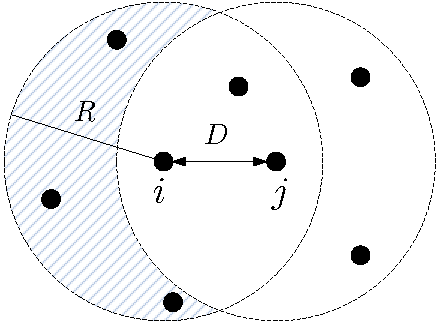
\includegraphics[width=5cm]{./model2.pdf}}
% \caption{The network model}\label{fig:model2}
% \end{figure}

 
% \subsection{อัลกอริทึม I}
% Add more subsections as you want.

%%%%%%%%%%%%%%%%%%%%%%%%%%%%%%%%%%%%%%%%%%%%%%%%%%%%%
%%%%%%%%%%%%%%%%%%%%%%%%%%%%%%%%%%%%%%%%%%%%%%%%%%%%%
%%%%%%%%%%%%%%%%%%%%%%%%%%%%%%%%%%%%%%%%%%%%%%%%%%%%%


\chapter{วิธีการดำเนินงาน}

\section{ข้อกำหนดและความต้องการของระบบ}
\begin{itemize}
  \item ผู้ใช้งานสามารถสมัครสมาชิกเพื่อเข้ามาใช้งานภายในระบบได้
  \item ผู้ใช้งานที่สมัครสมาชิกแล้ว สามารถเข้าสู่ระบบได้
  \item ผู้ใช้งานสามารถออกจากระบบได้
  \item ผู้ใช้งานสามารถค้นหาบทความตามหมวดหมู่ที่ต้องการค้นหาได้
  \item ผู้ใช้งานสามารถค้นหาบทความด้วยเลขอ้างอิงเนื้อหาได้
  \item สมาชิกสามารถตรวจสอบข้อมูลโปรไฟล์ของตนเองได้
  \item สมาชิกสามารถสร้างคำร้องขอเพื่อวิเคราะห์หมวดหมู่ของบทความด้วยการส่ง Web Link ให้กับระบบได้
  \item สมาชิกสามารถสร้างคำร้องขอเพื่อวิเคราะห์หมวดหมู่ของบทความด้วยการส่งบทความให้กับระบบได้
  \item สมาชิกสามารถสร้างคำร้องขอเพื่อวิเคราะห์หมวดหมู่ของบทความด้วยการส่ง Web Link ผ่าน Api-Key ให้กับระบบได้
  \item สมาชิกสามารถสร้างคำร้องขอเพื่อวิเคราะห์หมวดหมู่ของบทความด้วยการส่งบทความผ่าน Api-Key ให้กับระบบได้
  \item สมาชิกสามารถดูคำร้องขอการวิเคราะห์หมู่ของบทความของตนเองได้
  \item ระบบสามารถจัดหมวดหมู่ให้กับบทความได้ โดยการวิเคราะห์เนื้อหาภายในบทความ 
  \item ผู้จัดการระบบสามารถสามารถจัดการผู้ใช้งานและเนื้อหาได้
  \item ผู้จัดการระบบสามารถเพิ่มและจัดการหมวดหมู่ได้ด้วยตนเองผ่านทาง Frontend
\end{itemize}

\section{สถาปัตยกรรมระบบ}
\subsection{System Overview}
  \begin{figure}[!ht]\centering
    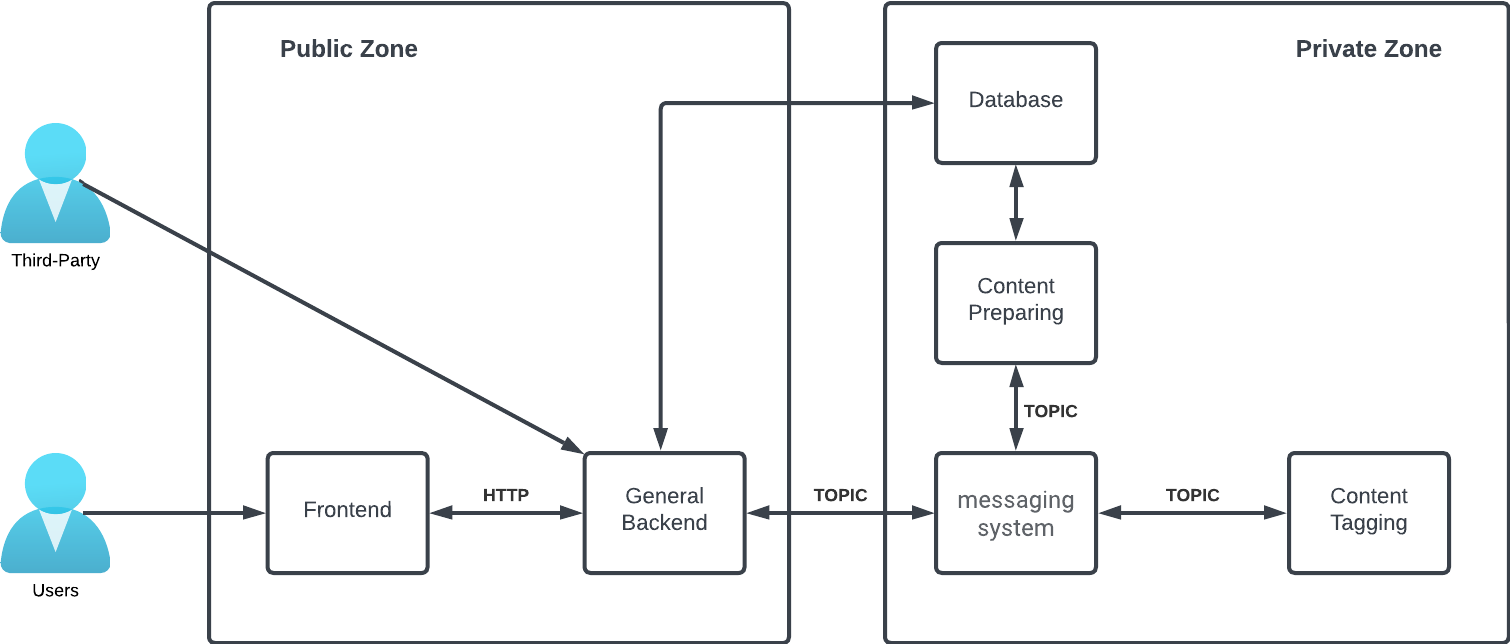
\includegraphics[width=\textwidth]{./img/architechture_simple.png}
    \caption{โครงสร้างทางสถาปัตยกรรมของระบบ}\label{fig:architecture_simple} 
  \end{figure}
  \newpage
  \hspace{1cm}ระบบจะถูกแบ่งเป็น 2 ส่วนหลัก ๆ ได้แก่ ส่วนที่ 1 จะเป็นส่วนที่ผู้ใช้งานสามารถเข้าถึงได้ 
  Ffpจะแบ่งเป็น Frontend ของเว็บไซต์และ Backend ของเว็บไซต์ที่จะประมวลผลเบื้องต้น เช่น การเข้าสู่ระบบหรือการสมัครสมาชิก 
  ซึ่งผู้ใช้งานจะสามารถติดต่อกับระบบได้ 2 วิธีด้วยกัน วิธีที่ 1 คือ การทำงานผ่านทางหน้าเว็บไซต์ โดยใช้ Email และ Password ในการเข้าสู่ระบบก่อนสร้างคำร้องขอต่าง ๆ 
  และวิธีที่ 2 คือ การใช้งานผ่าน Api-Key หรือเรียกว่า Third-Party ซึ่งจะติดต่อกับ Backend โดยตรง 
  โดย Backend จะส่งคำร้องขอไปยังส่วนที่ 2 ที่เป็นส่วนประมวลผลวิเคราะห์ข้อมูลและไม่สามารถเข้าถึงได้จากภายนอก 
  นอกจากนี้ระบบจะมีการสื่อสารระหว่างระบบด้วย Messaging System เพื่อให้สามารถทำงานแบบ Asynchronous ได้ 
  เนื่องจากการประมวลผลในแต่ละขั้นตอนอาจจะใช้เวลานาน การสื่อสารแบบ Asynchronous จะช่วยให้จัดการการทำงาน ไม่จำเป็นต้องรอให้ส่วนวิเคราะห์เสร็จสิ้นตามลำดับ 
  ทำให้สามารถประมวลผลส่วนอื่นได้ เมื่อประมวลผลเสร็จแล้ว ระบบก็จะส่งข้อมูลผ่าน Messaging System กลับมาซึ่งจะเป็นการทำงานแบบ Event Driver Architecture
  ซึ่งจะทำให้ระบบสามารถทำงานได้เร็วขึ้น และสามารถทำงานได้หลายอย่างพร้อมกันได้
  \begin{figure}[!ht]\centering
    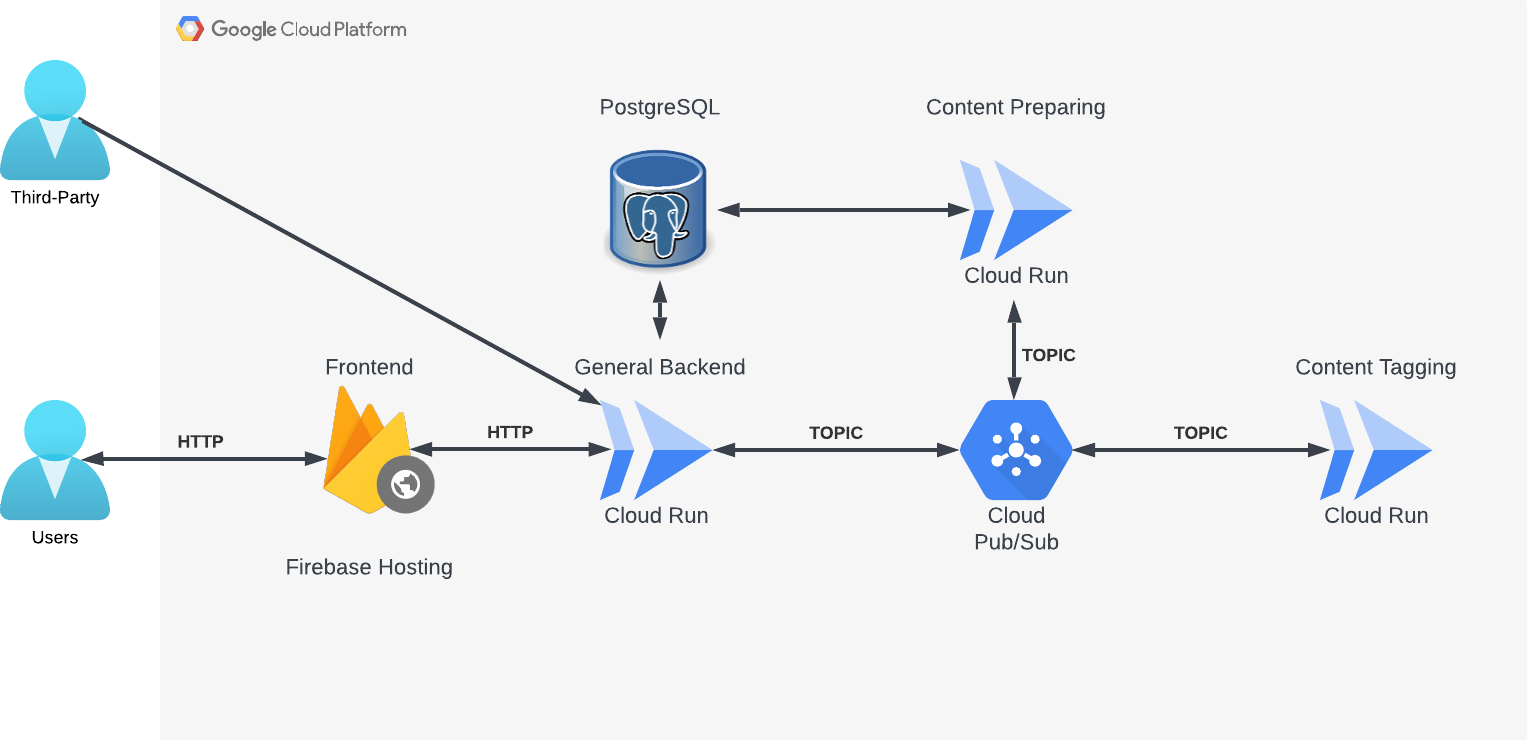
\includegraphics[width=\textwidth]{./img/architechture.png}
    \caption{เครื่องมือในโครงสร้างทางสถาปัตยกรรมของระบบ}\label{fig:architecture} 
  \end{figure}
  
  \hspace{1cm}จากภาพการออกแบบโครงสร้างทางสถาปัตยกรรมของระบบข้างต้น (รูปที่:\ref{fig:architecture}) ทำให้สามารถเลือกใช้เทคโนโลยีได้ดังภาพ ในส่วนของ Frontend จะใช้ Firebase Hosting 
  ในการนำเว็บไซต์ที่พัฒนาแล้ว ไปติดตั้งให้ผู้ใช้งานสามารถเข้าถึงได้ ในส่วนของ Server ประมวลผลต่าง ๆ จะมีการนำ Cloud Run มาใช้ในการประมวลผล 
  และในส่วนของ Messaging System จะใช้ Cloud Pub/Sub ซึ่งบริการทั้งหมดจะอยู่บน Google Cloud Platform 

\subsection{Content-Tagging}
  \hspace{1cm}ในส่วนของการนำโมเดลไป Deploy ใช้งานเป็นเว็บแอปพลิเคชันนั้น ต้องทำการแปลงโมเดลให้อยู่ในรูปแบบที่พร้อมนำไปใช้งาน 
  เช่น .joblib, .sav และ .h5 เมื่อนำเข้าโมเดลมายังเว็บแอปพลิเคชัน ขั้นตอนถัดไปคือการประมวลผลเกี่ยวกับการ Preprocessing 
  ซึ่งในขั้นตอนนี้ต้องทำเช่นเดิมเหมือนในช่วงการเตรียมข้อมูลสำหรับการพัฒนาโมเดล จากนั้นส่งข้อมูลที่ผ่านการ Preprocessing ให้โมเดลทำการทำนายผลลัพธ์ 
  โดยป้อน Input เป็นเนื้อหาต่าง ๆ และส่งผ่าน Cloud Pub/Sub เมื่อระบบประมวลผลเสร็จก็จะทำการส่งผลลัพธ์กลับไปยัง Cloud Pub/Sub 
  เพื่อให้ Service อื่น ๆ รับทราบและนำไปประมวลผลต่อไป

\subsection{Content-Preparing}
  \hspace{1cm}ในส่วนของการจัดเตรียมเนื้อหา (Content-Preparing) จะรับการส่งคำร้องขอวิเคราะห์หมวดหมู่ของบทความเข้ามาในระบบผ่าน Cloud Pub/Sub 
  จากนั้นจะทำการดักจับหน้าเว็บไซต์และดึงข้อมูลเฉพาะส่วนที่ต้องการ แล้วจึงทำการแปลภาษาเป็นภาษาอังกฤษเพื่อเก็บข้อมูลไปยังฐานข้อมูลและทำการกระจายข้อมูลไปยัง 
  Cloud Pub/Sub เพื่อให้ Service อื่น ๆ ได้ประมวลผลต่อ
\newpage
\subsection{General-Backend}
  \hspace{1cm}ในส่วนของการติดต่อกับ Frontend จะเป็นหน้าที่ของ General-Backend ซึ่งมีหน้าที่ต่าง ๆ เช่น การสมัครสมาชิก เข้าสู่ระบบ 
  และสำหรับการใช้งาน Cloud Pub/Sub ขั้นแรกจะต้องทำการสร้าง Topic สำหรับใช้เป็นหัวข้อในการกระจายข้อมูลไปยัง Subscriber ต่าง ๆ ที่ทำการ Subscribe กับ Topic นั้น ๆ
  ซึ่งหนึ่ง Topic สามารถมี Subscriber ได้หลายตัวโดยจะเป็นในลักษณะของ 1-to-Many ดังนั้นเมื่อมีข้อมูลที่ส่งมายัง Topic Cloud Pub/Sub จะทำการกระจายข้อมูลที่ได้รับไปยัง 
  Subscriber ทุก Subscriber ทำให้เมื่อมี Service อยากได้ข้อมูล ก็สามารถทำการ Subsriber ไปยัง Topic ที่ต้องการได้ทันที 
  ทำให้ระบบสามารถ Scale ฟังก์ชันการทำงานได้อย่างง่าย ไม่จำเป็นต้องเพิ่ม Code สำหรับการกระจายข้อมูลไปยังที่ใหม่
  \begin{figure}[!ht]\centering
    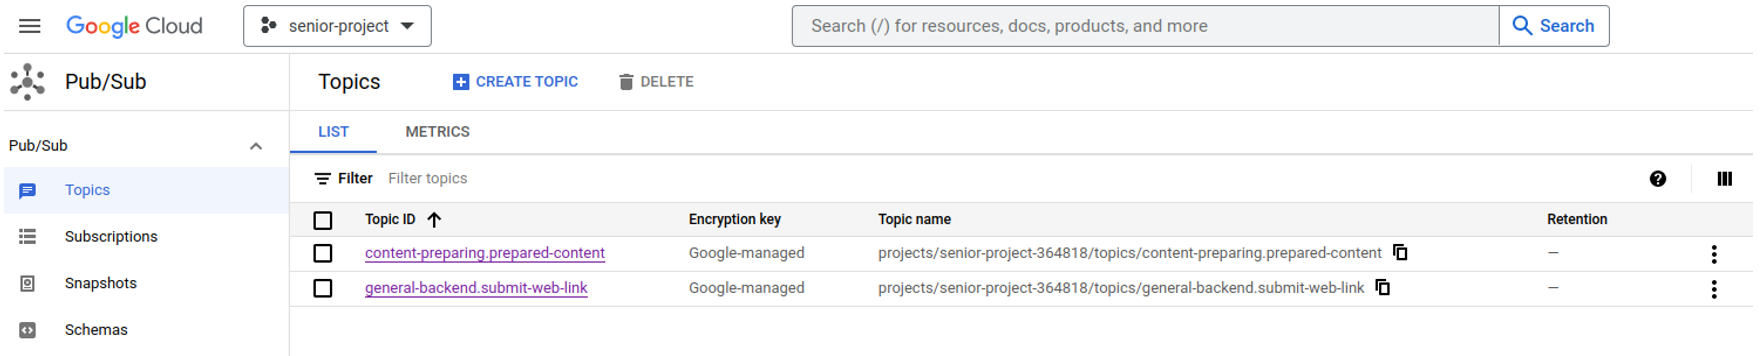
\includegraphics[width=\textwidth]{./img/topic.png}
    \caption{รายการ Topic ที่ใช้ในการสื่อสารในระบบ}\label{fig:topic_list}
  \end{figure}

  \hspace{1cm}เนื่องจาก Service ทำงานโดยใช้บริการ Cloud Run ทำให้สามารถ Monitor การใช้งานต่าง ๆ เช่น Memory, CPU ได้ 
  \begin{figure}[!ht]\centering
    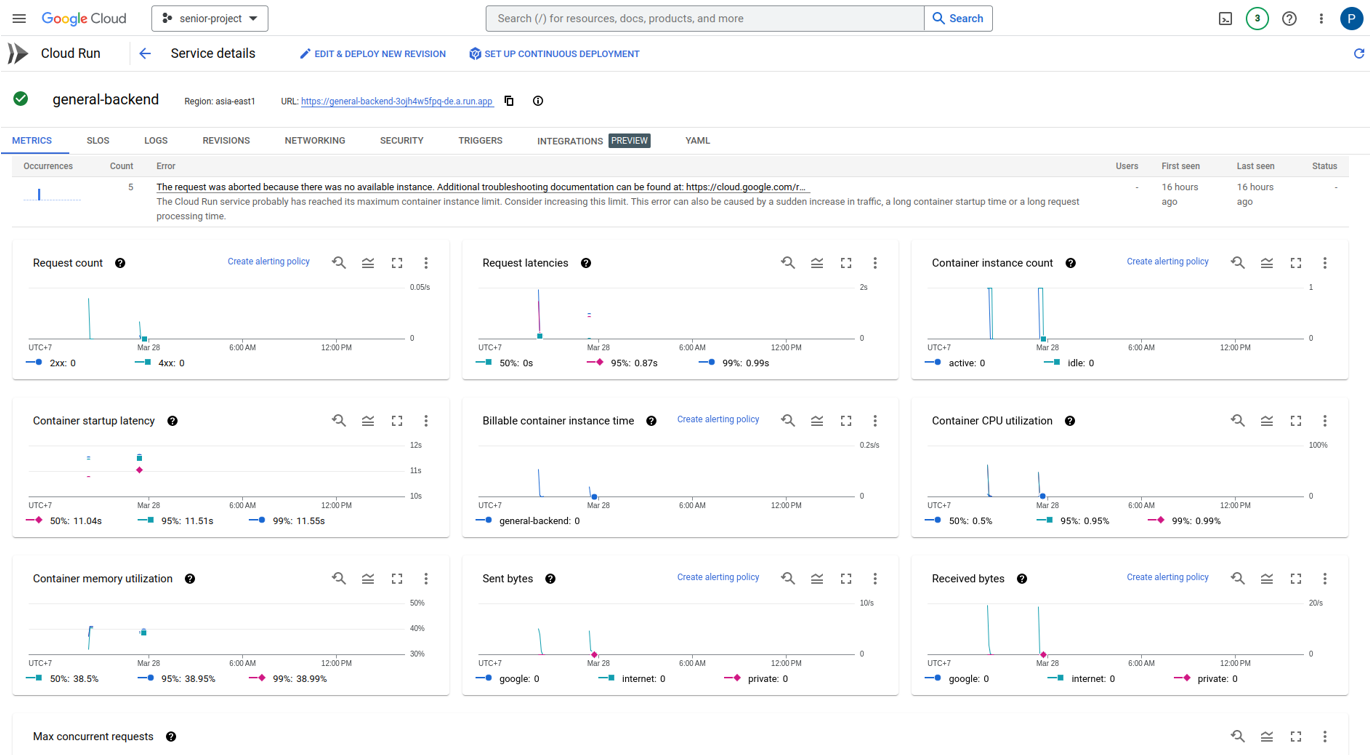
\includegraphics[width=\textwidth]{./img/monitor.png}
    \caption{การ Monitor การใช้งานทรัพยากรต่าง ๆ บน Cloud Run}\label{fig:monitor}
  \end{figure}
  \newpage    
  \begin{figure}[!ht]\centering
    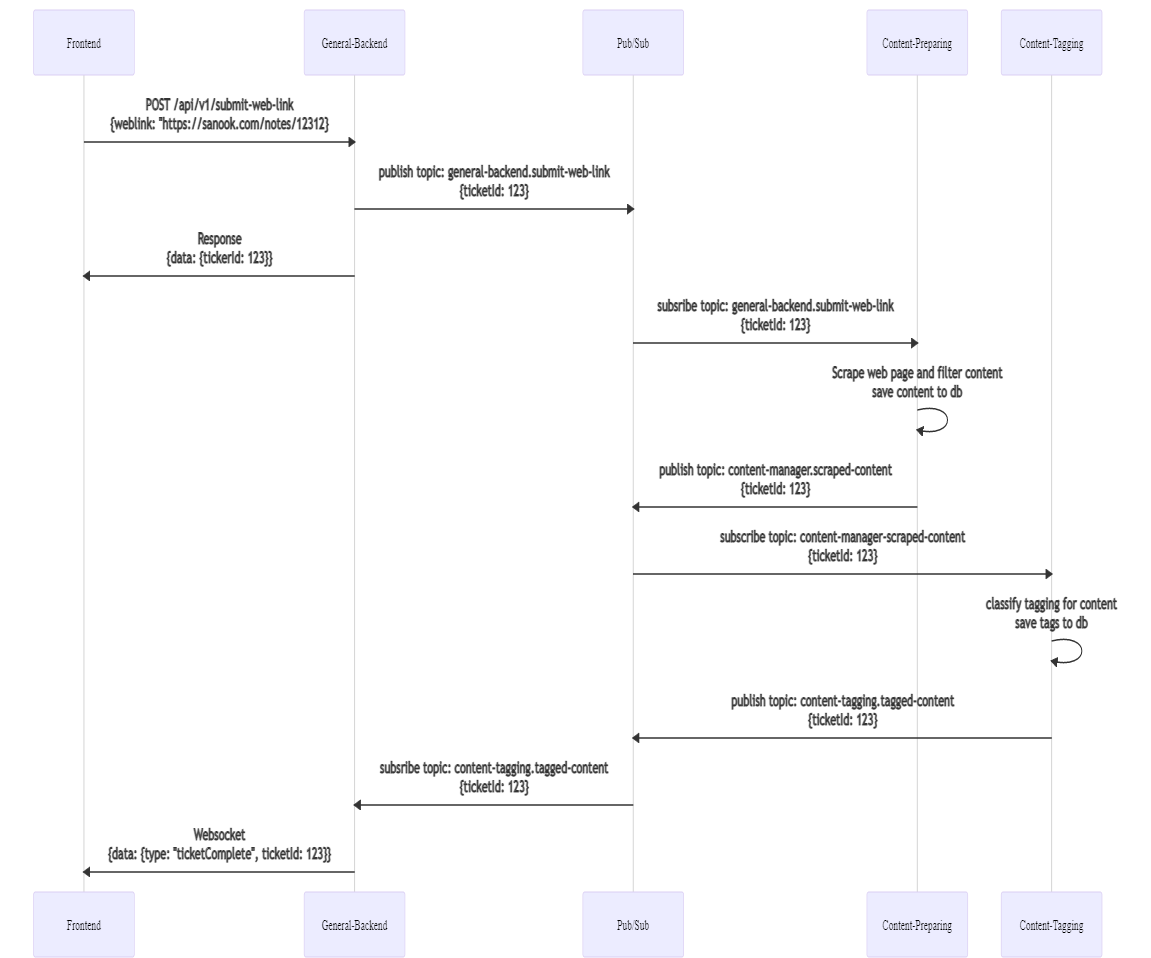
\includegraphics[width=\textwidth]{./img/request_process_flow.png}
    \caption{Sequence Diagram จำลองการส่งประมวลผลการวิเคราะห์หมวดหมู่ของบทความ}\label{fig:req_proc} 
  \end{figure}
  
  \hspace{1cm}ภาพข้างต้น (รูปที่:\ref{fig:req_proc}) คือ Time Sequence จำลองการส่งประมวลผลวิเคราะห์หมวดหมู่ของบทความ โดยจะเริ่มจาก Frontend ส่งคำร้องขอมายัง Backend 
  จากนั้น Backend จะ Publish ข้อมูลไปยัง Cloud Pub/Sub และเข้าสู่กระบวนการวิเคราะห์ข้อมูล โดยเริ่มจากการที่ระบบ Content-Preparing จะทำการไปเก็บข้อมูลจากเว็บไซต์ปลายทาง 
  ได้แก่ หัวข้อและเนื้อหา แล้วจึงส่งกลับมายัง Cloud Pub/Sub ซึ่งระบบ Content-Tagging จะทำการนำเนื้อหาที่ได้ไปวิเคราะห์ต่อไป และเมื่อกระบวนการทั้งหมดเสร็จสิ้น ก็จะทำการส่งกลับมายัง Backend 
  แล้วจึงส่งต่อให้ Frontend ต่อไป
  \newpage
  \begin{figure}[!ht]\centering
    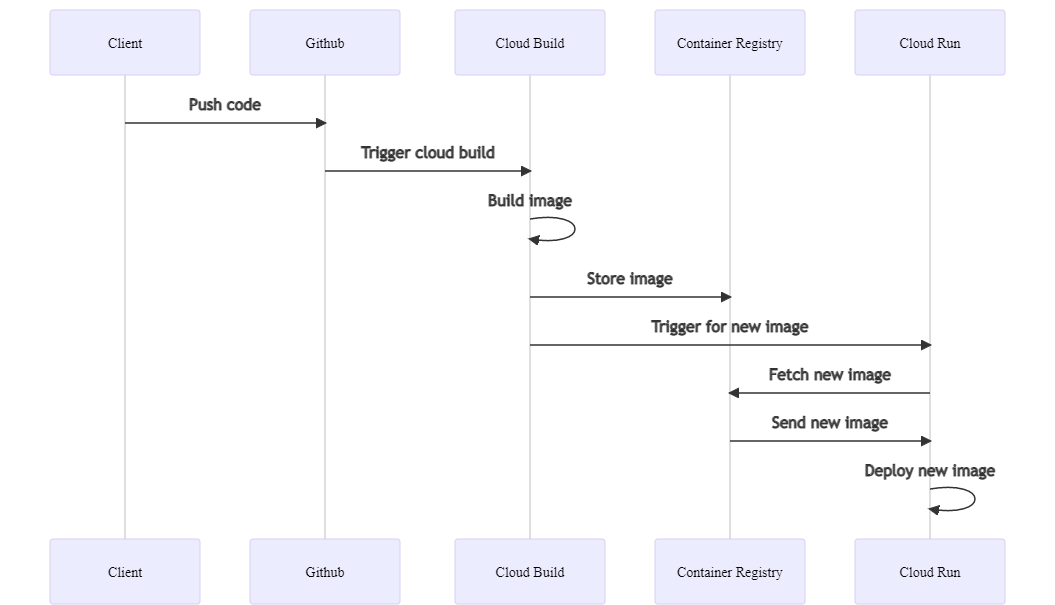
\includegraphics[width=0.8\textwidth]{./img/devops.png}
    \caption{Sequence Diagram ของ DevOps Life Cycle}\label{fig:devops} 
  \end{figure}
  
  ในส่วนของกระบวนการพัฒนาและติดตั้งระบบสำหรับใช้งาน (รูปที่:\ref{fig:devops}) จะใช้เทคโนโลยีหลัก ๆ ได้แก่ 
  \newline\hspace*{0.5cm} 1. Github สำหรับเก็บ Source Code และเมื่อมีการ Push Code ใหม่ขึ้นมา จะส่งผลให้เกิดการ Trigger ไปยัง Cloud Build
  \newline\hspace*{0.5cm} 2. Cloud Build จะทำการดึง Source Code จาก Github และทำการ Build เป็น Container Image สำหรับสร้าง Application ในรูปแบบของ Container และจะส่งไปเก็บไว้ใน Container Registry
  \newline\hspace*{0.5cm} 3. Container Registry จะเป็นส่วนที่เก็บ Image ของ Application ที่ต้องการในไปทำงาน ซึ่งจะถูก Cloud Run นำไปสร้างเป็น Container สำหรับประมวลผลต่อไป
  \newline\hspace*{0.5cm} 4. Cloud Run จะเป็น Serverless สำหรับประมวลผลคำร้องขอต่าง ๆ 
  
  \begin{figure}[!ht]\centering
    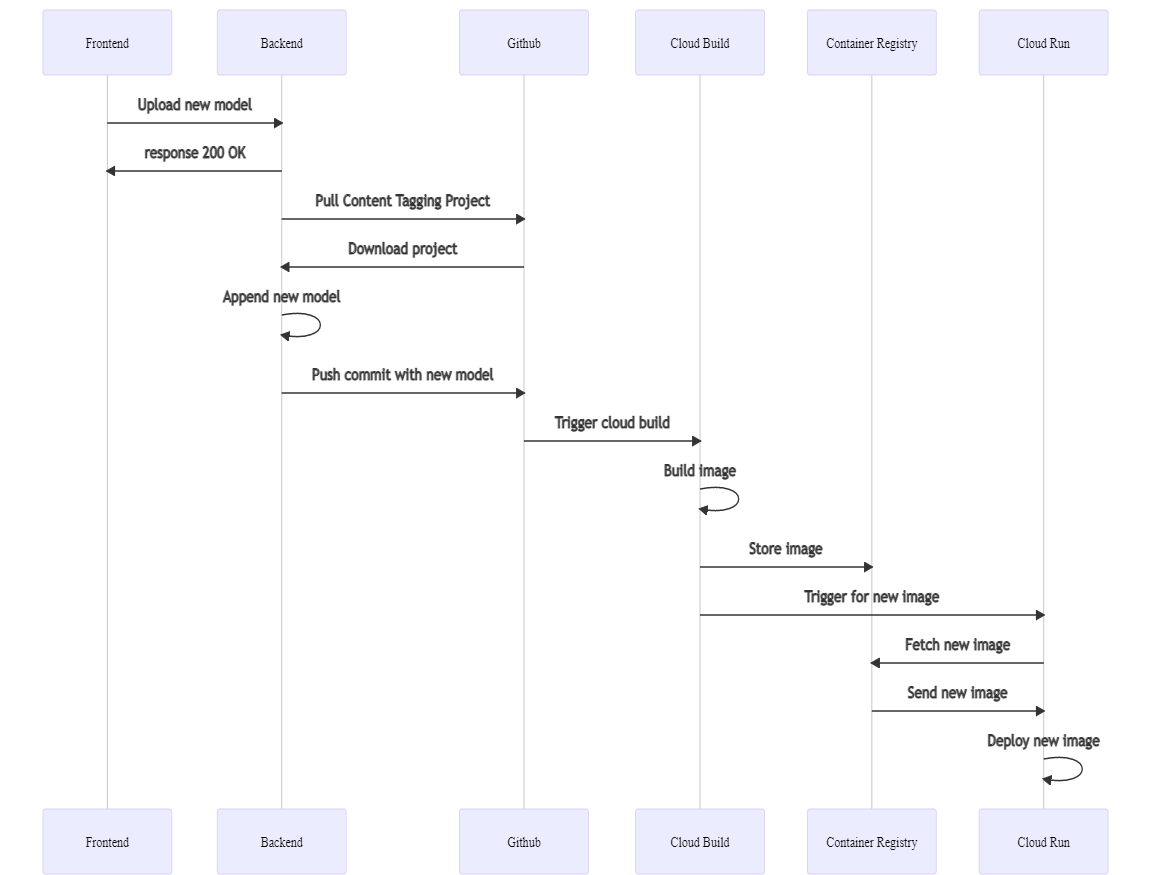
\includegraphics[width=0.9\textwidth]{./img/ai_update.png}
    \caption{Sequence Diagram ของ Update New AI-Model Process}\label{fig:ai_update} 
  \end{figure}
  
  \hspace{1cm} จากภาพข้างต้น (รูปที่:\ref{fig:ai_update}) ในส่วนของการแก้ไข Model ของ AI จะทำในลักษณะที่ใช้กระบวนการ DevOps โดยที่จะทำการอัพโหลด Model ใหม่ผ่าน Admin UI 
  จากนั้น Backend จะทำการ Clone โครงการของ Content-Tagging และนำไฟล์ที่อัพโหลดผ่าน Admin UI เพิ่มเข้าไป แล้วจึงทำการ Push Code กลับมายัง Github 
  จากนั้น Pipeline ของการ Deploy ก็จะทำการ Trigger แล้วจึงทำงานต่อไปจน Deploy ขึ้นไปยัง Cloud Run 

\subsection{Navigation Map}
  \begin{figure}[!ht]\centering
    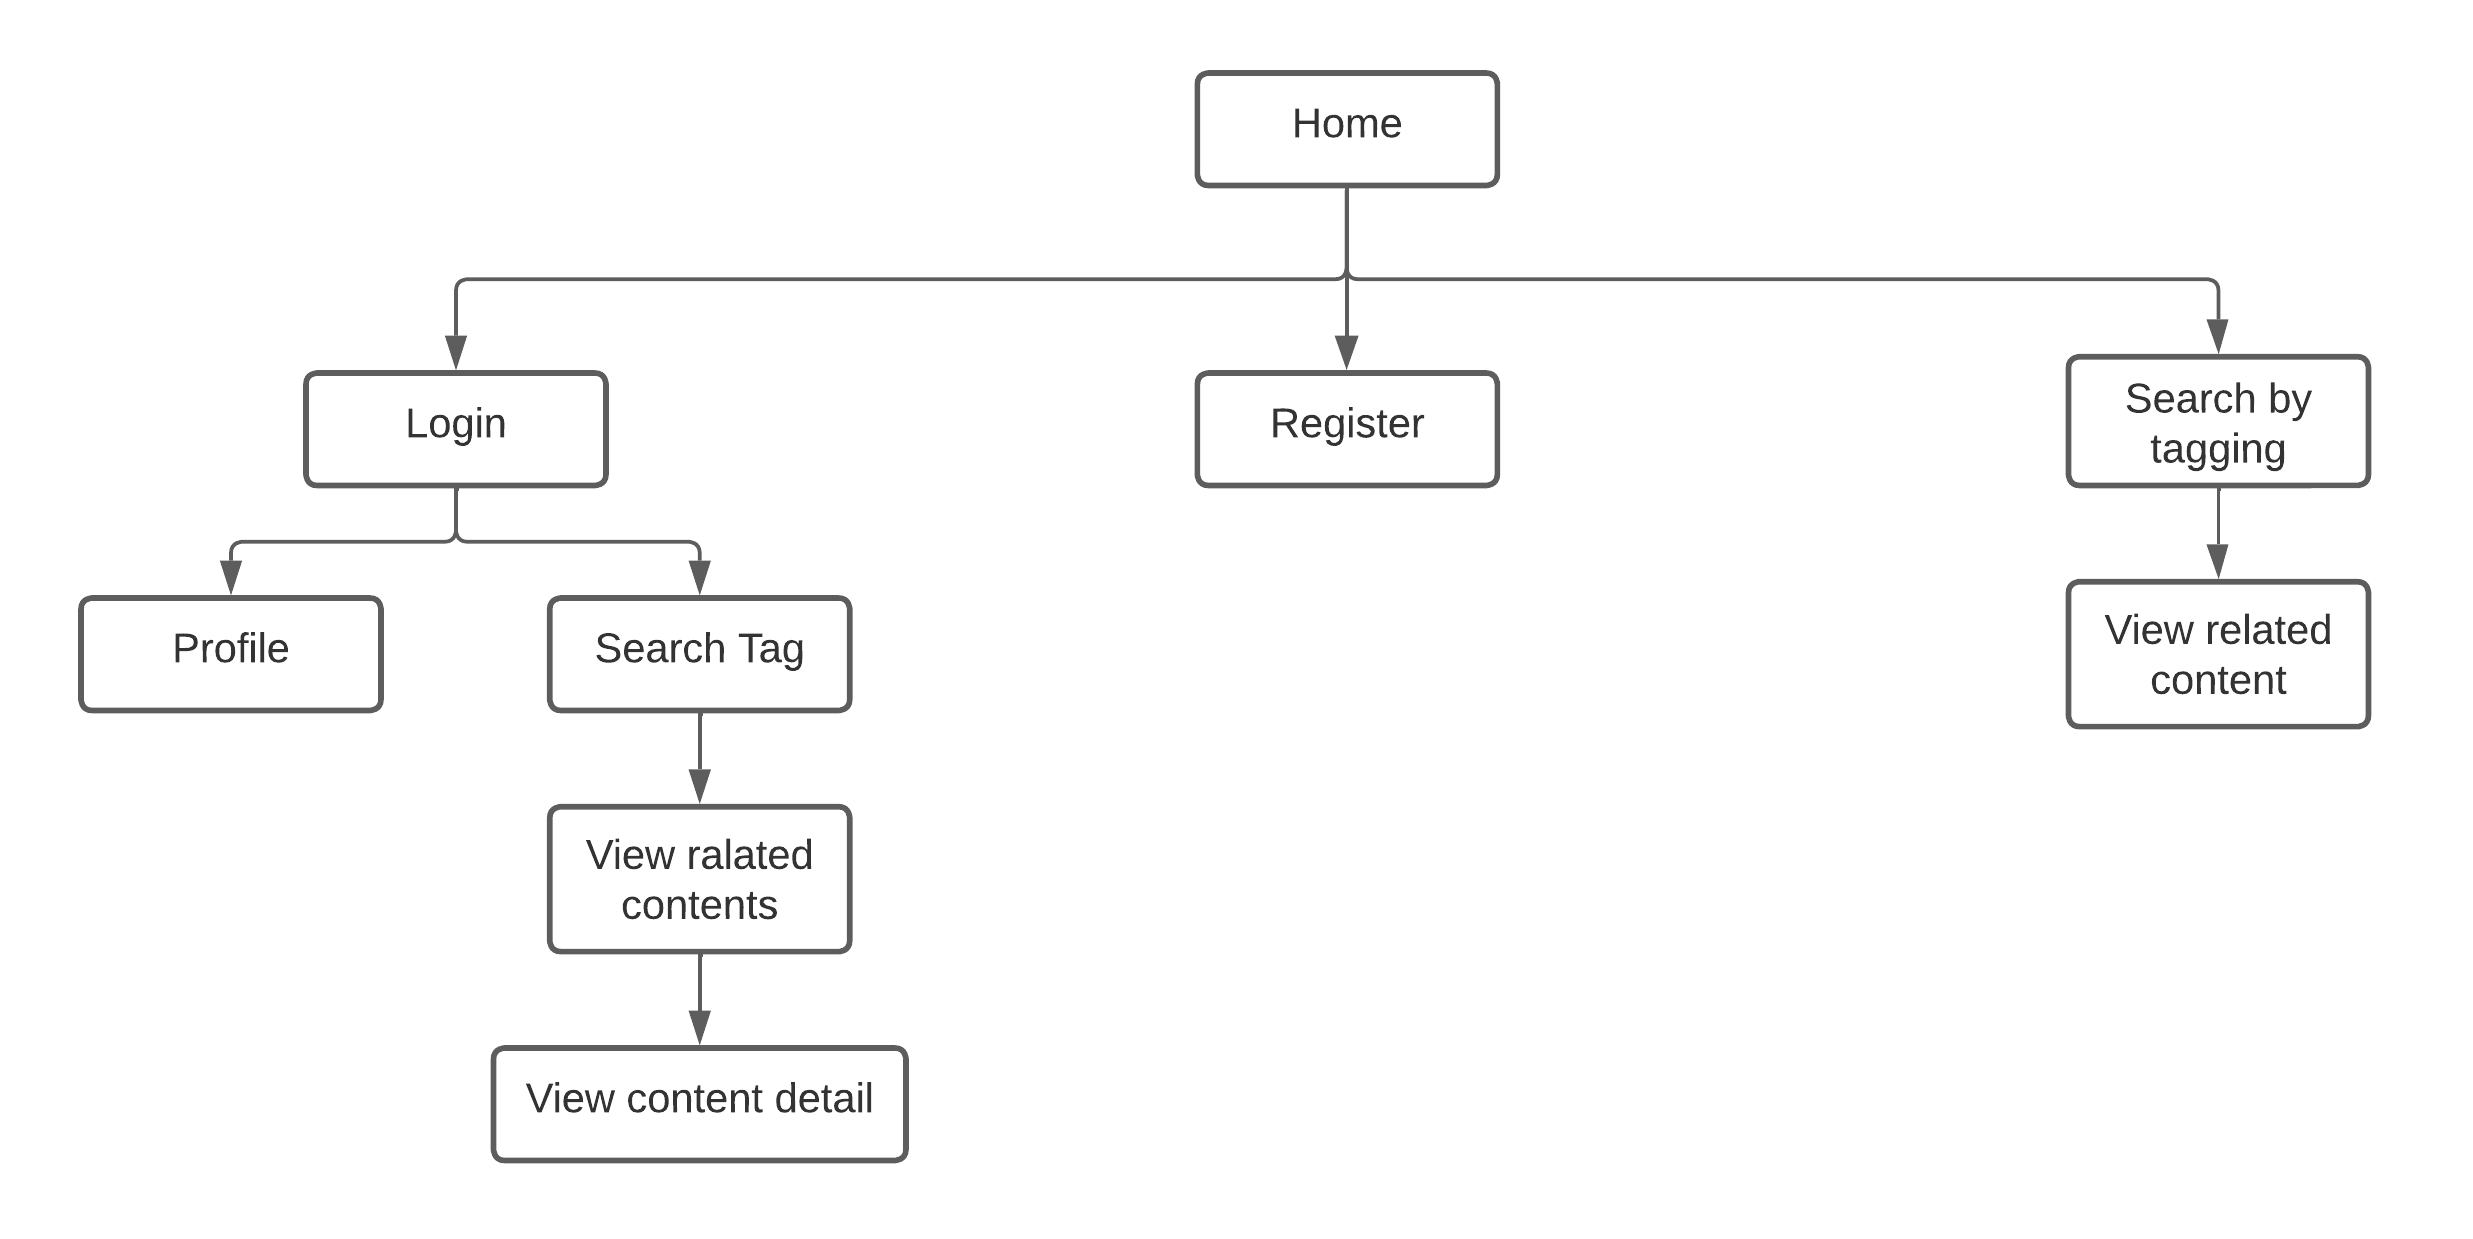
\includegraphics[width=13cm]{./img/nav.png}
    \caption{Navigation Map ของเว็บไซต์สำหรับผู้ใช้งาน}\label{fig:navmap} 
  \end{figure}

  \hspace{1cm}เมื่อผู้ใช้งานเข้าใช้งานเว็บไซต์ AI Platform Thai Content Tagging เว็บไซต์จะเริ่มต้นที่หน้า Landing ซึ่งหน้า Landing จะประกอบไปด้วยรายละเอียดต่าง ๆ เกี่ยวกับเว็บไซต์ AI Platform Thai Content Tagging 
  ได้แก่ ข้อมูลภาพรวมของเว็บไซต์ กระบวนการในการประมวลผลหมวดหมู่โดย AI และวิธีการใช้งานการวิเคราะห์หมวดหมู่ของบทความ โดยในหน้า Landing ระบบจะแบ่งออกเป็น 3 ทางเลือก ได้แก่ 
  หน้า Register สำหรับผู้ใช้งานที่ยังไม่มีบัญชีในระบบ หน้า Login สำหรับผู้ใช้งานที่มีบัญชีในระบบแล้ว และหน้า Search By Tagging สำหรับผู้ใช้งานที่ต้องการค้นหาบทความ
  ผู้ใช้งานที่ต้องการใช้งานจำเป็นที่จะต้องมีบัญชีในการใช้งานจึงจะสามารถเข้าสู่ระบบเพื่อรับบริการได้ เมื่อเข้าสู่ระบบแล้ว ผู้ใช้งานจะสามารถส่งคำร้องขอเพื่อขอการวิเคราะห์หมวดหมู่ของบทความที่ต้องการได้ 2 วิธี คือ Web Link และ Raw Content 
  เมื่อส่งคำร้องขอวิเคราะห์หมวดหมู่ของบทความแล้ว ระบบจะทำการประมวลผลและจะขึ้นสถานะให้ผู้ใช้งานได้ทราบ หากคำร้องขอการวิเคราะห์สำเร็จ ผู้ใช้งานจะสามารถค้นหาบทความด้วยหมวดหมู่และสามารถดูบทความที่เกี่ยวข้องเพิ่มเติมได้
  นอกจากนี้ผู้ใช้งานยังสามารถจัดการโปรไฟล์ของตนเองได้และสามารถดูประวัติการร้องขอของตนเองได้เช่นกัน
  \begin{figure}[!ht]\centering
    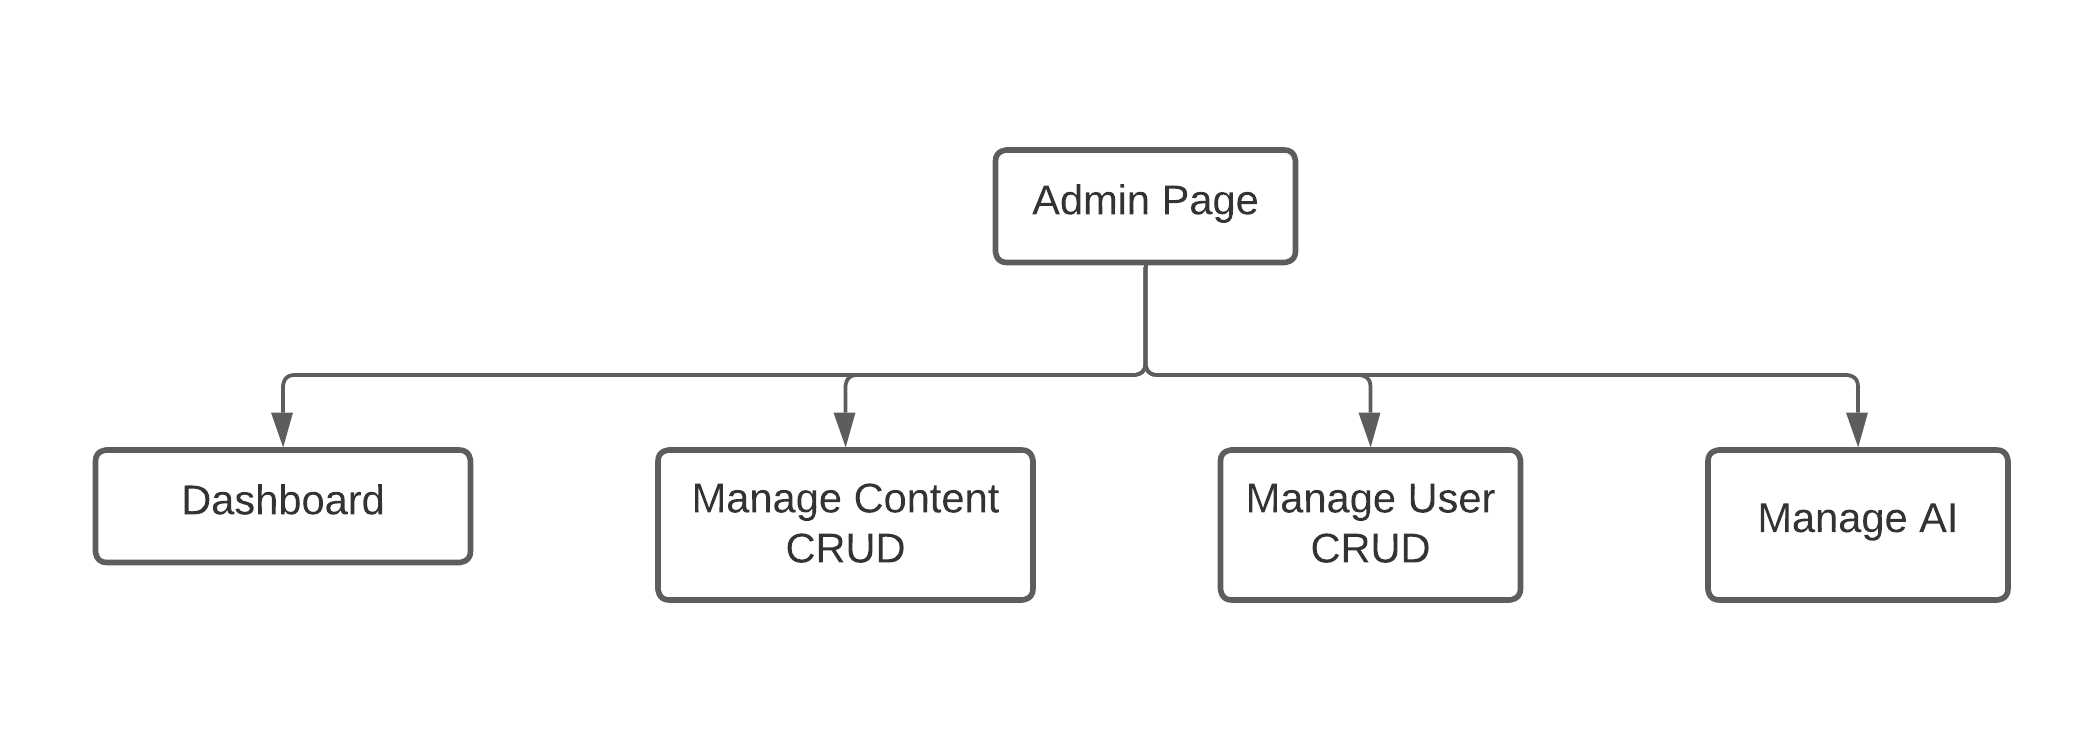
\includegraphics[width=13cm]{./img/nav_admin.png}
    \caption{Navigation Map ของเว็บไซต์สำหรับผู้จัดการระบบ}\label{fig:navmap_admin} 
  \end{figure}
  \newline\hspace*{1cm}ในส่วนของผู้จัดการระบบ จะเป็นส่วนที่จัดการระบบหลังบ้านของเว็บไซต์ทั้งหมด เช่น จัดการข้อมูลผู้ใช้งาน เนื้อหาที่ผู้ใช้งานได้ส่งคำร้องขอ ซึ่งสามารถเข้าถึงได้เฉพาะผู้จัดการระบบเท่านั้น
  
  \newpage
  \subsection{Data Science Processing}
  \begin{figure}[!ht]\centering
    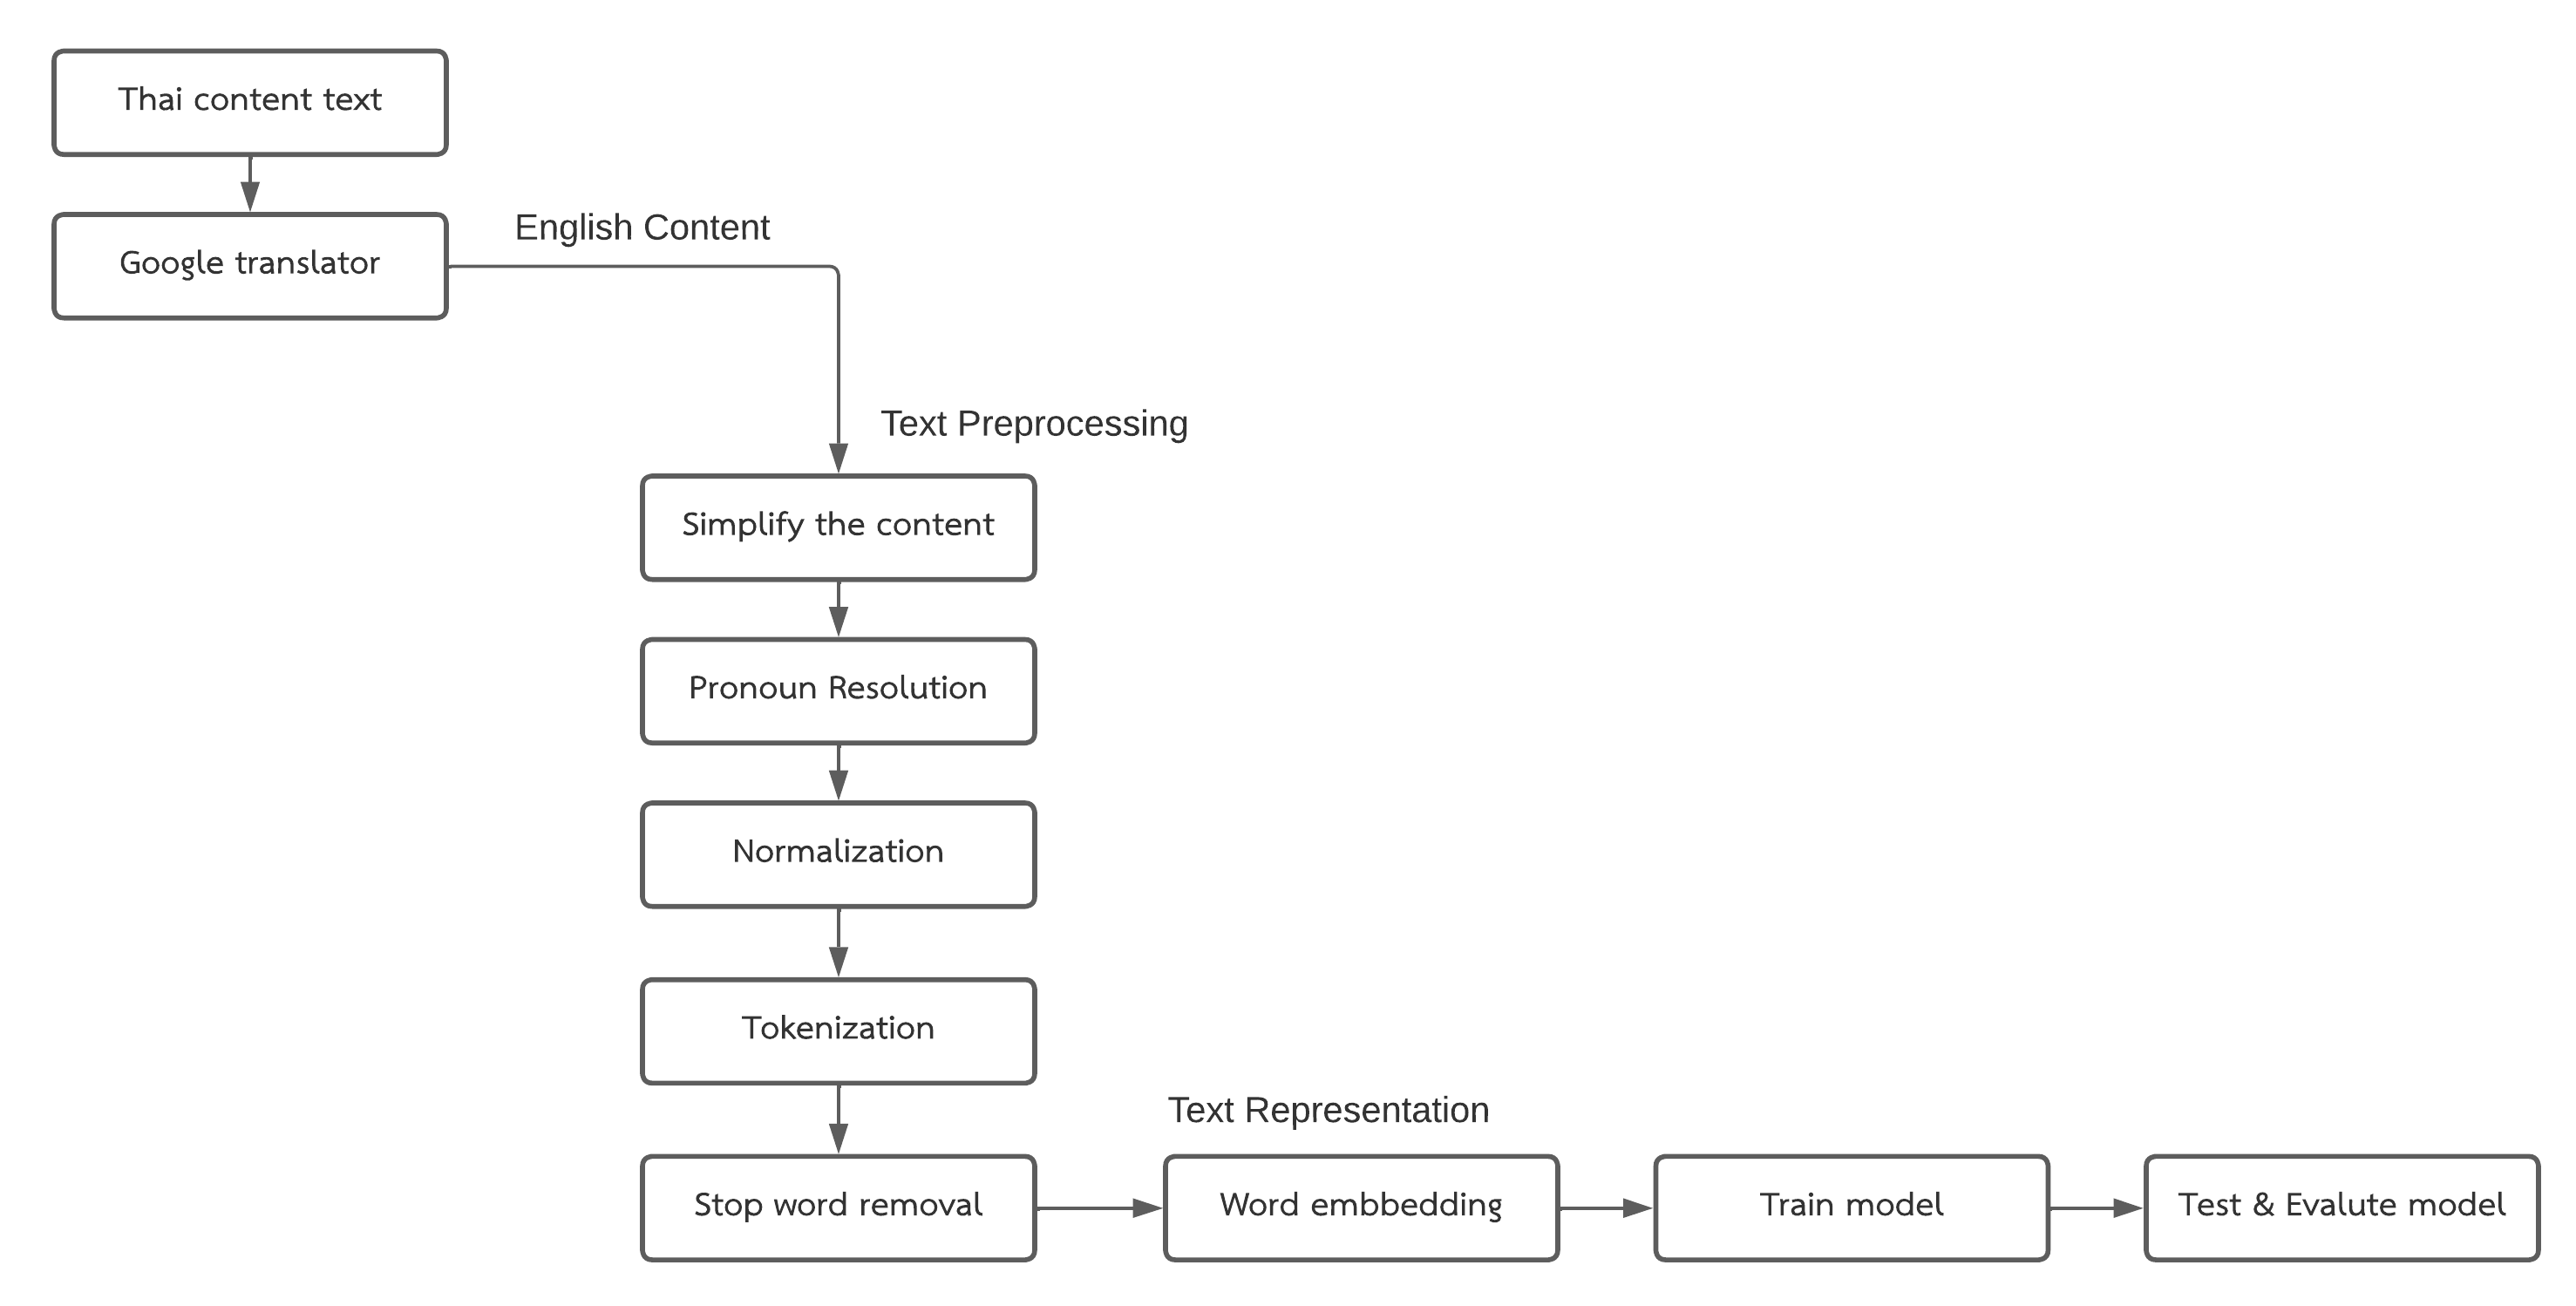
\includegraphics[width=\textwidth]{./img/data_proc.png}
    \caption{Data Processing}\label{fig:data_proc} 
  \end{figure}

  \hspace{1cm}ในกระบวนการทำโมเดลจะมีขั้นตอนหลัก ๆ ดังนี้
  \begin{enumerate}
    \item การเตรียมข้อมูลสำหรับทำโมเดล
          \newline\hspace*{1cm}ในขั้นตอนของการเตรียมข้อมูลสำหรับทำโมเดล จะมีทั้งหมด 2 ขั้นตอนหลัก ๆ ด้วยกัน ได้แก่
          \begin{enumerate}
            \item การรวบรวมข้อมูลบทความต่าง ๆ จากแพลตฟอร์มออนไลน์ เช่น เว็บ Sanook, Thai PBS หรือไทยรัฐ ด้วยการทำ Web Scraping 
            โดยการใช้ Selenium เป็น Web Driver และใช้ BeautifulSoup ในการดึงข้อมูลผ่านทางหน้าเว็บไซต์และสกัดเอาเฉพาะส่วนที่ต้องการออกมา 
            ได้แก่ ส่วนหัวข้อและส่วนเนื้อหาของบทความ ซึ่งจะได้บทความจากเว็บไซต์ที่มีเนื้อหาเป็นภาษาไทยออกมา
            จากนั้นจึงรวบรวมเป็นไฟล์ข้อความตามหมวดหมู่ โดยรวบรวมหมวดหมู่ละ 1,500 ชุด
            \item เนื่องจากมีจำนวนเครื่องมิอสำหรับการพัฒนาโมเดลที่รองรับและจัดการข้อมูลที่เป็นภาษาอังกฤษได้มากกว่าภาษาไทย
            ดังนั้นคณะผู้จัดทำจึงเลือกที่จะใช้ข้อมูลทั้ง 2 ภาษาสำหรับการพัฒนาโมเดล ได้แก่ ภาษาไทยและภาษาอังกฤษ 
            และเปรียบเทียบผลลัพธ์ว่าชุดข้อมูลภาษาใดส่งผลให้โมเดลมีประสิทธิภาพสูงที่สุด 
            ซึ่งชุดข้อมูลที่เป็นภาษาอังกฤษจะได้มาจากการนำบทความภาษาไทยที่ทำการรวบรวมด้วยการทำ Web Scraping
            มาแปลงเป็นภาษาอังกฤษด้วยบริการของ Google Translator แล้วจึงนำข้อมูลไปใช้ในกระบวนการถัดไป
          \end{enumerate}
    \item การทำ Text Preprocessing
          \begin{enumerate}
            \item ทำความสะอาดข้อมูล คือ ทำการเปลี่ยนตัวอักษรให้เป็นตัวพิมพ์เล็กทั้งหมด ตัดอักขระพิเศษที่ไม่ใช่ตัวอักษรภาษาอังกฤษออก เช่น อิโมจิ ตัวเลข หรือ Punctuation 
            และลบเว้นวรรคที่ติดกันมากกว่า 1 เว้นวรรคเพื่อให้เหลือเว้นวรรคเดียว ซึ่งการทําในลักษณะนี้จะเป็นการลดสัญญาณรบกวนในข้อมูล
            \item Tokenization คือ การแยกคำแต่ละคำในประโยคออกจากกัน โดยที่ยังมีความหมายถูกต้องสมบูรณ์ตามฐานข้อมูลพจนานุกรม 
            ดังนั้นจึงใช้ word\_tokenize ใน Library NLTK ในการช่วยแบ่งคำในประโยค
            \item การลบ Stop Word คือ การลบคำทั่วไปที่พบได้บ่อยในประโยคออก ซึ่งเป็นคำที่ไม่ค่อยสื่อความหมายในประโยค เช่น a, also, unless 
            เพื่อให้เหลือเพียงคำที่ค่อนข้างสื่อความหมายและมีความสำคัญในประโยค โดยใช้ Library NLTK ในการเรียกใช้ Stop Words 
            \item Normalization คือ การลดความซับซ้อนของคำให้อยู่ในรูปของคำพื้นฐาน เพื่อกำจัด Inflection ของคำ 
            เพื่อลดความซับซ้อนของการนำไปประมวลผล Model ด้วยการใช้ Lemmatization จาก Library Spacy 
            เพื่อให้คำที่มีความหมายเหมือนกันอยู่ในรูปเดียวกัน เช่น is am are เป็น be จากนั้นจึงรวมคำทุกคำให้กลายเป็นประโยคเพื่อนำไปใช้ในขั้นตอนถัดไป
          \end{enumerate}
    \item การทำ Text Representation คือ การแปลงคำให้เป็น Vector ที่อยู่ในรูปตัวเลขเพื่อนำมาใช้ในการพัฒนาโมเดล 
          ซึ่งคณะผู้จัดทำได้เลือกใช้หลักการ TF-IDF ในการคำนวณหาค่าความสำคัญของคำแต่ละคำในชุดข้อมูล
          แล้วจึงแทนข้อความด้วยตัวเลขที่เป็นค่าความสำคัญของคำในแต่ละคำ เพื่อทำ Text Representation ให้เป็น Vector
          โดยใช้ TfidfVectorizer ใน Library Scikit-Learn ในการสร้างโมเดล TF-IDF สำหรับแปลงข้อความเป็น Vector 
          และปรับ tune พารามิเตอร์เพื่อให้ได้ผลลัพธ์ที่ดีที่สุด ซึ่งพารามิเตอร์ที่ต้องปรับ tune มีดังนี้
          \begin{itemize}
            \item min\_df คือ พารามิเตอร์ที่ใช้กำหนดค่าความถี่ของคำต่ำสุดที่จะถือว่าสำคัญพอที่จะนำมาใช้ในการสร้ง Text Representation 
                  โดยมีค่าเป็นจำนวนเต็มบวกหรือเป็นสัดส่วนที่ระบุจำนวนคำที่ต้องปรากฏในเอกสารอย่างน้อยกี่ครั้งถึงจะถือว่าเป็นคำที่สำคัญพอที่จะนำมาใช้ในการคำนวณ TF-IDF
                  ทำให้คำที่ปรากฏในเอกสารถ้าน้อยกว่าค่า min\_df จะไม่ถูกนับเข้าไปในการคำนวณ TF-IDF ซึ่งจะช่วยลดคำที่ไม่สำคัญและเพิ่มความสัมพันธ์กับคำที่มีความถี่สูงมากขึ้น
            \item max\_df คือ พารามิเตอร์ที่ใช้กำหนดค่าความถี่ของคำสูงสุดที่จะถือว่าเป็นคำที่ไม่สำคัญมากพอที่จะนำมาใช้ในการสร้าง Text Representation 
                  โดยมีค่าเป็นจำนวนเต็มบวกหรือเป็นสัดส่วนที่ระบุจำนวนคำที่ต้องปรากฏในเอกสารมากที่สุดกี่ครั้งถึงจะถือว่าเป็นคำที่ไม่สำคัญพอที่จะนำมาใช้ในการคำนวณ TF-IDF
                  ทำให้คำที่ปรากฏในเอกสารถ้ามากกว่าค่า max\_df จะไม่ถูกนับเข้าไปในการคำนวณ TF-IDF ซึ่งจะช่วยลดคำที่ไม่สำคัญและเพิ่มความสัมพันธ์กับคำที่มีความถี่สูงต่ำลง
            \item max\_features คือ พารามิเตอร์ที่ใช้กำหนดจำนวนคำสูงสุดที่จะใช้ในการสร้าง Text Representation 
                  โดยมีค่าเป็นจำนวนเต็มบวกที่ระบุจำนวนคำสูงสุดที่ต้องการให้เป็น feature ในโมเดล
                  เมื่อกำหนดค่า max\_features ไว้ใน TfidfVectorizer โมเดลจะเลือกเฉพาะคำที่ถูกเลือกมาจากข้อมูลในจำนวนที่กำหนด 
                  ซึ่งจำนวนคำที่ถูกเลือกจะเป็นคำที่มีความถี่สูงสุดตามลำดับจนถึงค่า max\_features
                  หากมีข้อมูลมากและมีคำซ้ำกันมาก ๆ ค่า max\_features ควรเลือกสูง เพื่อให้ feature มีความหลากหลายมากขึ้น
            \item norm คือ พารามิเตอร์ที่ใช้กำหนดวิธีการปรับค่าขนาดของเวกเตอร์ TF-IDF หลังจากที่คำนวณค่า TF-IDF ของแต่ละคำในเอกสาร
            \item stop\_words คือ รายการคำ stopwords ที่ต้องการให้ตัดออกในการคำนวณค่า TF-IDF
            \item ngram\_range คือ จำนวนคำติดกันที่นำมาใช้ในการคำนวณค่า TF-IDF
          \end{itemize}
    \item การพัฒนาโมเดล Model
          \newline\hspace*{1cm}เป็นการสร้างโมเดล ซึ่งจะทำทั้งหมด 3 โมเดลด้วยกัน ได้แก่ Random Forest, K-Nearest Neighbor และ LSTM
          โดยแต่ละโมเดลจะมีขั้นตอนในการพัฒนาโมเดล ดังนี้
          \begin{itemize}
            \item Random Forest
                  \begin{enumerate}
                    \item แบ่งชุดข้อมูลออกเป็น 2 ส่วน ส่วนแรกสำหรับการพัฒนาโมเดลและส่วนที่สองสำหรับการประเมินโมเดล 
                    ซึ่งจะแบ่งชุดข้อมูลแต่ละรูปแบบออกเป็นอัตราส่วน 8:2 (ชุดข้อมูลสำหรับการพัฒนาโมเดล : ชุดข้อมูลสำหรับการประเมินโมเดล) 
                    \item นำชุดข้อมูลสำหรับการพัฒนาโมเดลมาแปลงเป็น Vector ด้วยโมเดล TF-IDF ที่สร้างไว้ เพื่อใช้ในการพัฒนาโมเดล
                    \item สร้างโมเดลสำหรับทำ Text Classification โดยใช้ RandomForestClassifier ใน Library Scikit-Learn 
                          และปรับ tune พารามิเตอร์เพื่อให้ได้ผลลัพธ์ที่ดีที่สุด ซึ่งพารามิเตอร์ที่ต้องปรับ tune มีดังนี้
                          \begin{itemize}
                            \item n\_estimators คือ จำนวน Decision Tree ที่จะถูกปรับแต่งและนำมาใช้ในการทำนายหรือตัดสินใจในการจัดกลุ่ม (Classification) ใน Random Forest
                                  ซึ่งการกำหนดค่า n\_estimators ควรพิจารณาความซับซ้อนของปัญหา ขนาดข้อมูลที่ใช้ในการฝึกโมเดล และเวลาที่ใช้ในการสร้างและทำนาย 
                                  โดยค่าที่เหมาะสมสำหรับ n\_estimators อาจแตกต่างกันไปในแต่ละงานหรือปัญหาที่ต้องการใช้ Random Forest 
                                  ดังนั้นจึงต้องมีการทดลองและทดสอบการใช้งานกับค่า n\_estimators ต่าง ๆ เพื่อหาค่าที่เหมาะสม
                            \item max\_depth คือ จำนวนชั้นของ Decision Tree ที่ถูกสร้างขึ้นในโมเดล Random Forest ซึ่งการกำหนดค่า max\_depth จะส่งผลในการควบคุมความซับซ้อนของโมเดล
                                  ดังนั้นจึงต้องมีการทดลองและทดสอบการใช้งานกับค่า max\_depth ต่าง ๆ เพื่อหาค่าที่เหมาะสม
                            \item min\_samples\_split คือ จำนวนตัวอย่างขั้นต่ำที่จำเป็นต้องมีในโหนดก่อนที่จะทำการแยกสร้างโหนดย่อยใน Decision Tree ที่ถูกสร้างขึ้นในโมเดล Random Forest
                                  ซึ่งการกำหนดค่า min\_samples\_split สามารถช่วยลดความซับซ้อนของต้นไม้และป้องกันการเกิด Overfitting
                                  ดังนั้นจึงต้องมีการทดลองและทดสอบการใช้งานกับค่า min\_samples\_split ต่าง ๆ เพื่อหาค่าที่เหมาะสม
                            \item min\_samples\_leaf คือ จำนวนตัวอย่างขั้นต่ำที่จำเป็นต้องมีในโหนดย่อยสุดท้ายของ Decision Tree 
                                  ซึ่งการกำหนดค่า min\_samples\_split ควรพิจารณาความซับซ้อนของปัญหา ขนาดข้อมูลที่ใช้ในการฝึกโมเดล 
                                  และความต้องการในการควบคุมความลึกและการแยกสร้างโหนดย่อยใน Random Forest
                                  ดังนั้นจึงต้องมีการทดลองและทดสอบการใช้งานกับค่า min\_samples\_leaf ต่าง ๆ เพื่อหาค่าที่เหมาะสม
                          \end{itemize}
                    \item นำชุดข้อมูลที่แปลงเป็น Vector มาทำการ fit กับโมเดลที่สร้างไว้
                  \end{enumerate}
            \item K-Nearest Neighbor
                  \begin{enumerate}
                    \item แบ่งชุดข้อมูลออกเป็น 2 ส่วน ส่วนแรกสำหรับการพัฒนาโมเดลและส่วนที่สองสำหรับการประเมินโมเดล 
                    ซึ่งจะแบ่งชุดข้อมูลแต่ละรูปแบบออกเป็นอัตราส่วน 8:2 (ชุดข้อมูลสำหรับการพัฒนาโมเดล : ชุดข้อมูลสำหรับการประเมินโมเดล) 
                    \item นำชุดข้อมูลสำหรับการพัฒนาโมเดลมาแปลงเป็น Vector ด้วยโมเดล TF-IDF ที่สร้างไว้ เพื่อใช้ในการพัฒนาโมเดล
                    \item สร้างโมเดลสำหรับทำ Text Classification โดยใช้ KNeighborsClassifier ใน Library Scikit-Learn 
                          และปรับ tune พารามิเตอร์เพื่อให้ได้ผลลัพธ์ที่ดีที่สุด ซึ่งพารามิเตอร์ที่ต้องปรับ tune มีดังนี้
                          \begin{itemize}
                            \item n\_neighbors คือ การกำหนดจำนวนเพื่อนบ้านที่ใช้ในการพิจารณาเพื่อตัดสินใจในการจัดกลุ่มหรือทำนายค่าของตัวอย่างใหม่
                                  จากนั้นจะใช้วิธีการหาค่าเฉลี่ยหรือการโหวตเพื่อตัดสินใจในการจัดกลุ่มหรือทำนายค่าของตัวอย่างใหม่
                                  ดังนั้นจึงต้องมีการทดลองและทดสอบการใช้งานกับค่า n\_neighbors ต่าง ๆ เพื่อหาค่าที่เหมาะสม
                            \item weights คือ การกำหนดน้ำหนักให้กับตัวอย่างในกระบวนการคำนวณระยะห่างหรือความคล้ายคลึงใน K-Nearest Neighbor
                                  ซึ่งจะมีทั้งหมด 2 ค่า ได้แก่ uniform ที่ทำให้ตัวอย่างทุกตัวจะมีน้ำหนักเท่ากัน ไม่สนใจระยะห่างระหว่างตัวอย่าง
                                  และ distance ที่ทำให้ตัวอย่างใกล้ที่สุดจะมีน้ำหนักมากกว่าตัวอย่างที่ห่างออกไป
                          \end{itemize}
                    \item นำชุดข้อมูลที่แปลงเป็น Vector มาทำการ fit กับโมเดลที่สร้างไว้
                  \end{enumerate}
            \item LSTM
                  \begin{enumerate}
                    \item แบ่งชุดข้อมูลออกเป็น 2 ส่วน ส่วนแรกสำหรับการพัฒนาโมเดลและส่วนที่สองสำหรับการประเมินโมเดล 
                    ซึ่งจะแบ่งชุดข้อมูลแต่ละรูปแบบออกเป็นอัตราส่วน 8:2 (ชุดข้อมูลสำหรับการพัฒนาโมเดล : ชุดข้อมูลสำหรับการประเมินโมเดล) 
                    \item นำชุดข้อมูลสำหรับการพัฒนาโมเดลมาแปลงเป็น Vector ด้วยโมเดล TF-IDF ที่สร้างไว้ เพื่อใช้ในการพัฒนาโมเดล
                    \item สร้างโมเดลสำหรับทำ Text Classification ทั้งหมด 3 Layer ได้แก่ Embedding Layer, LSTM Layer และ Dense Layer
                          โดยใช้ Embedding, LSTM และ Dense ใน Library Tensorflow ตามลำดับ
                          จากนั้นจึงทำการ Compile โมเดลด้วย Optimizer
                          โดยในทุก Layer จะต้องมีการปรับ tune พารามิเตอร์เพื่อให้ได้ผลลัพธ์ที่ดีที่สุด ซึ่งพารามิเตอร์ที่ต้องปรับ tune มีดังนี้
                          \begin{itemize}
                            \item units คือ จำนวนของ Nueral ที่มีใน LSTM Layer
                            \item dropout คือ อัตราส่วนที่จะทำการสุ่มลบบางส่วนของ Nueral ใน LSTM Layer 
                                  ซึ่งช่วยลดการเกิด Overfitting และช่วยให้โมเดลทำนายและทำงานกับข้อมูลที่ไม่เคยเห็นมาก่อนได้ดีขึ้น
                            \item activation คือ ฟังก์ชันที่ใช้ในการปรับข้อมูลหลังจากผ่านการคำนวณเพื่อสร้างผลลัพธ์ออกมา 
                                  ซึ่งในโมเดลนี้จะเลือกใช้ Softmax เนื่องจากเป็นการคำนวณผลลัพธ์จากหลายผลลัพธ์ที่ได้ทำการเรียนรู้
                            \item optimizers คือ อัลกอริทึมที่ใช้ในกระบวนการปรับค่าพารามิเตอร์ของโมเดลในระหว่างการฝึกสอน เพื่อลดค่าของ Loss Function 
                                  และปรับปรุงประสิทธิภาพของโมเดลให้ดีขึ้น ซึ่งการเลือก optimizers ที่เหมาะสมขึ้นอยู่กับปัญหาที่กำลังจะแก้ไขและลักษณะของข้อมูล 
                                  ดังนั้นจึงต้องทพการทดลองและประเมินผลลัพธ์ของโมเดลกับ optimizers ต่างๆเพื่อหาวิธีการปรับแต่งที่ให้ผลลัพธ์ที่ดีที่สุด
                            \item loss คือ ตัวชี้วัดที่ใช้ในการประเมินความคลาดเคลื่อนระหว่างผลลัพธ์ที่โมเดลทำนายกับผลลัพธ์จริงในขณะฝึกสอน 
                                  โดยค่า loss จะแสดงถึงความต่างหรือความสูญเสียระหว่างค่าที่โมเดลทำนายได้กับค่าจริงของข้อมูลฝึกสอน
                                  ซึ่งในโมเดลนี้จะเลือกใช้ Categorical Cross-Entropy เนื่องจากเป็นฟังก์ชันสำหรับงานที่เกี่ยวกับการจำแนกหลายคลาส 
                                  ใช้ในการคำนวณค่าความคลาดเคลื่อนระหว่างความน่าจะเป็นที่ทำนายได้กับความน่าจะเป็นจริงของแต่ละคลาส
                            \item learning\_rate คือ ค่าที่ใช้ในการกำหนดอัตราการปรับค่าพารามิเตอร์ในกระบวนการฝึกสอนของโมเดล 
                                  อัตราการเรียนรู้จะมีผลต่อความเร็วและความน่าเชื่อถือในการปรับปรุงโมเดล
                                  ดังนั้นจึงต้องทพการทดลองและประเมินผลลัพธ์ของโมเดลกับ learning\_rate ต่างๆเพื่อหาวิธีการปรับแต่งที่ให้ผลลัพธ์ที่ดีที่สุด
                          \end{itemize}
                    \item นำชุดข้อมูลที่แปลงเป็น Vector มาทำการ fit กับโมเดลที่สร้างไว้
                  \end{enumerate}
          \end{itemize}
    \item การทดสอบและประเมินผลโมเดล 
          \newline\hspace*{1cm}เป็นการทดสอบและวัดผลประสิทธิภาพของโมเดล โดยในที่นี้จะวัดผลด้วยการใช้ค่า Accuracy, Precision, Recall และ F1 Score
  \end{enumerate}
  \newpage

\section{Use Case Analysis}
\subsection{Use Case Diagram}
\begin{figure}[!ht]\centering
  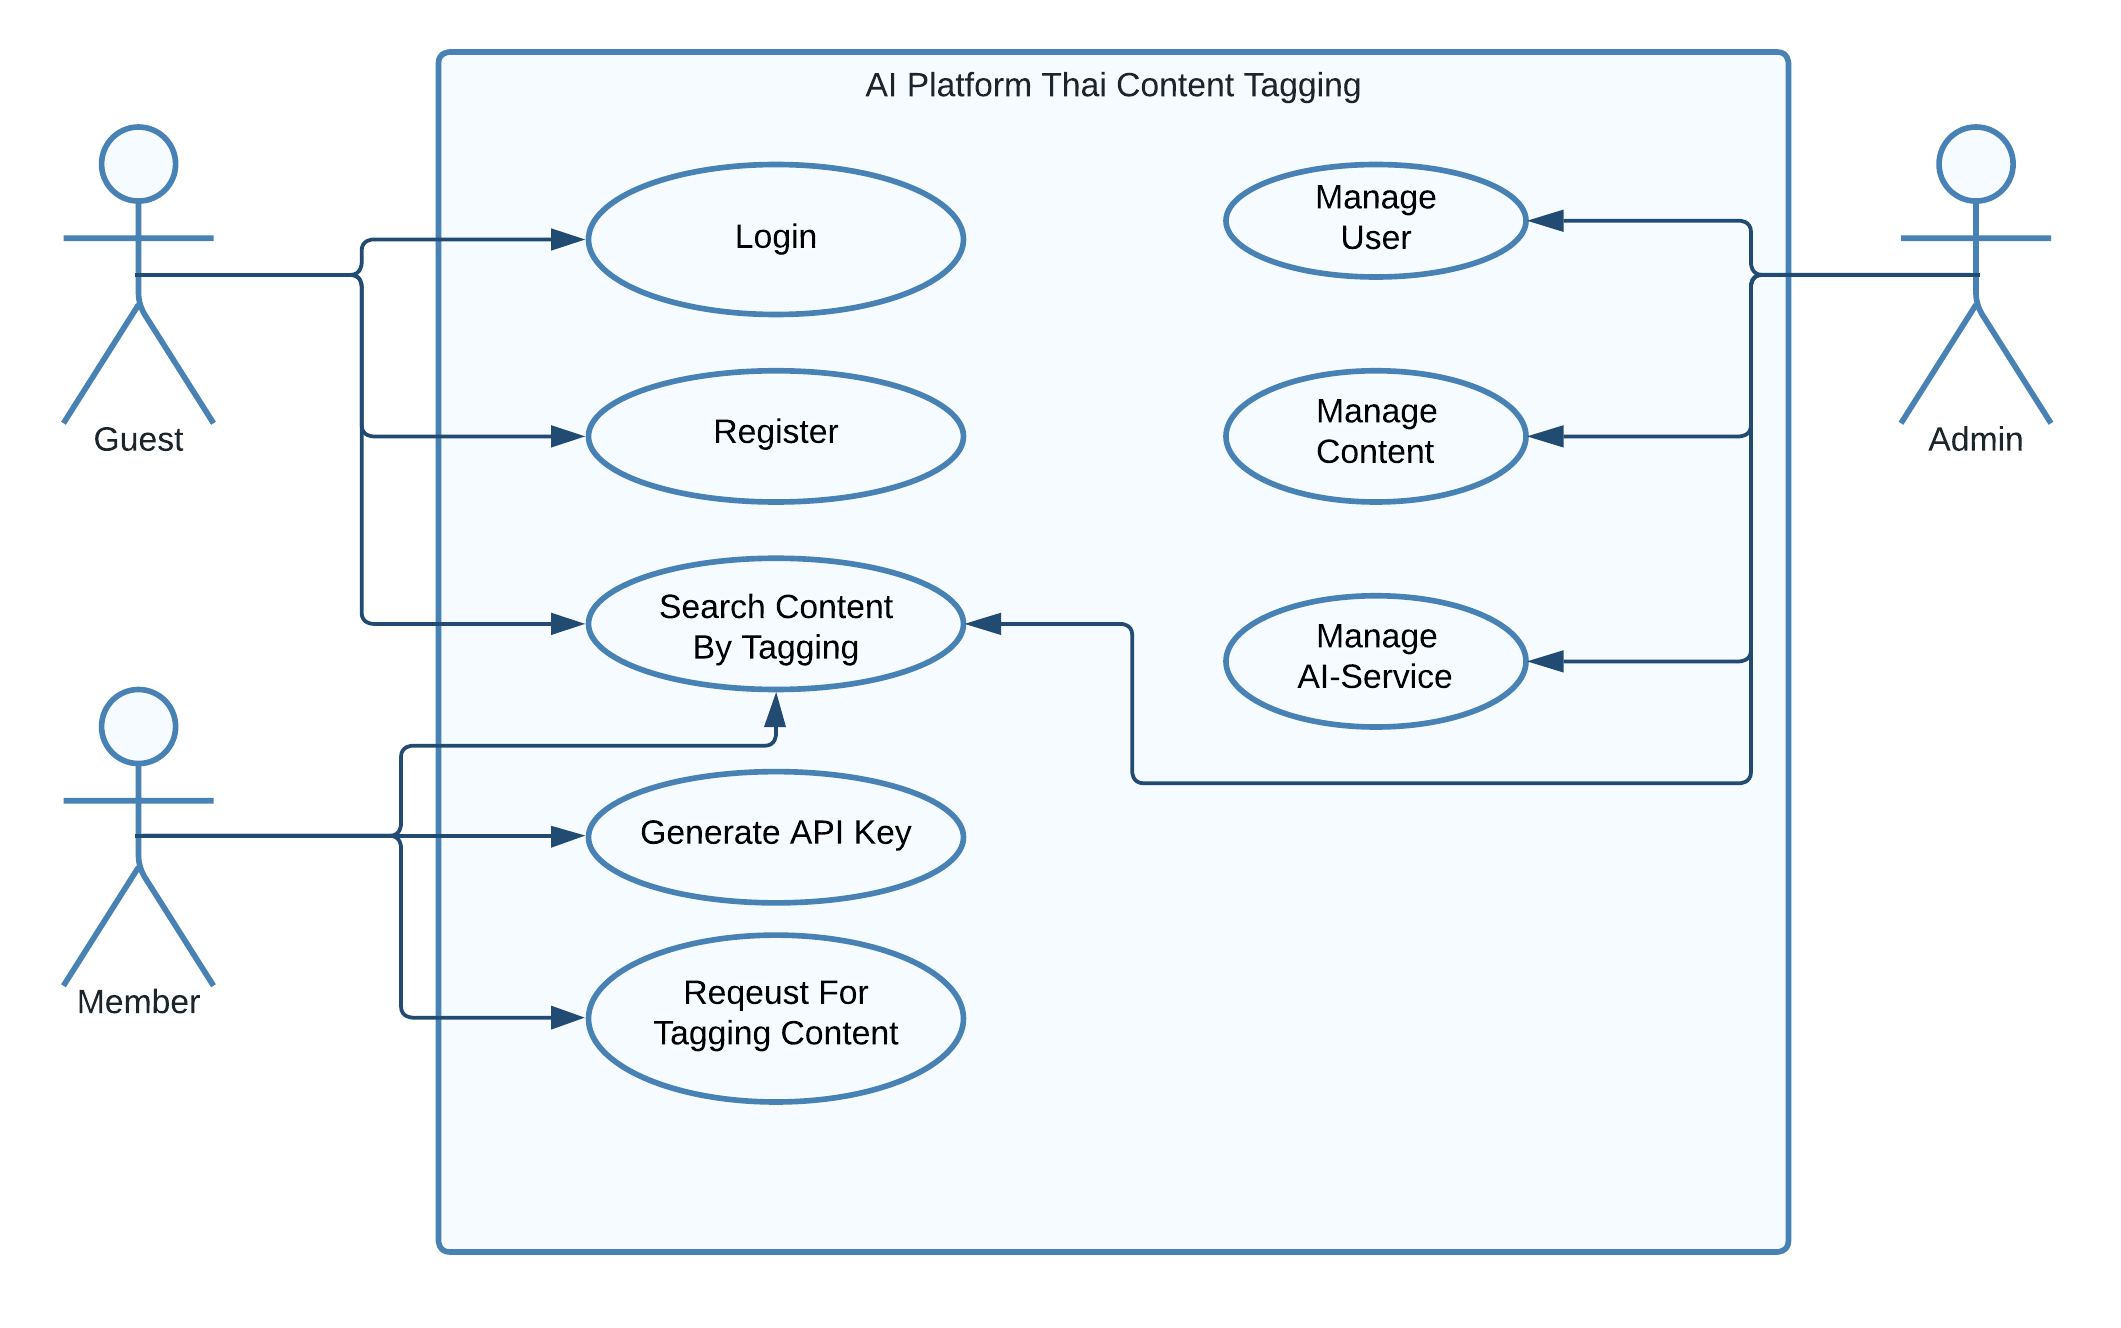
\includegraphics[width=13cm]{./img/usecase.png}
  \caption{Use Case Diagram}\label{fig:usecase} 
\end{figure}

\subsection{Use Case Narrative}

\subsubsection{ผู้ใช้งานสมัครสมาชิก}
\textbf{Name: }ผู้ใช้งานสมัครสมาชิก \\
\textbf{Actors: }ผู้ใช้งานทั่วไป \\
\textbf{Goal: }ผู้ใช้งานต้องการสมัครสมาชิกกับระบบ \\
\textbf{Precondition: }- \\
\textbf{Main success scenario: } \\
  \hspace*{0.5cm}1. ผู้ใช้งานกรอกข้อมูลส่วนตัว รวมไปถึง Email และ Password \\
  \hspace*{0.5cm}2. ผู้ใช้งานส่งแบบฟอร์มข้อมูลมายังระบบ \\
  \hspace*{0.5cm}3. ระบบตรวจสอบข้อมูลและทำการบันทึกลงฐานข้อมูล \\
  \hspace*{0.5cm}4. ผู้ใช้งานลงทะเบียนเสร็จวมบูรณ์ \\
\textbf{Extension (a): } \\
  \hspace*{0.5cm}3a. ระบบตรวจสอบข้อมูลพบว่าผู้ใช้งานกรอกข้อมูลไม่ครบ \\
  \hspace*{0.5cm}4a. ผู้ใช้งานได้รับแจ้งเตือนว่ากรอกข้อมูลไม่ครบ \\
  \hspace*{0.5cm}5a. กลับไปที่ข้อที่ 1 \\
\textbf{Extension (b): }  \\
  \hspace*{0.5cm}3a. ระบบตรวจสอบข้อมูลพบว่ามี Email อยู่แล้วในระบบ \\
  \hspace*{0.5cm}4a. ผู้ใช้งานได้รับแจ้งเตือนว่า Email ซ้ำ \\
  \hspace*{0.5cm}5a. กลับไปที่ข้อที่ 1 
\newpage
\begin{figure}[!ht]\centering
  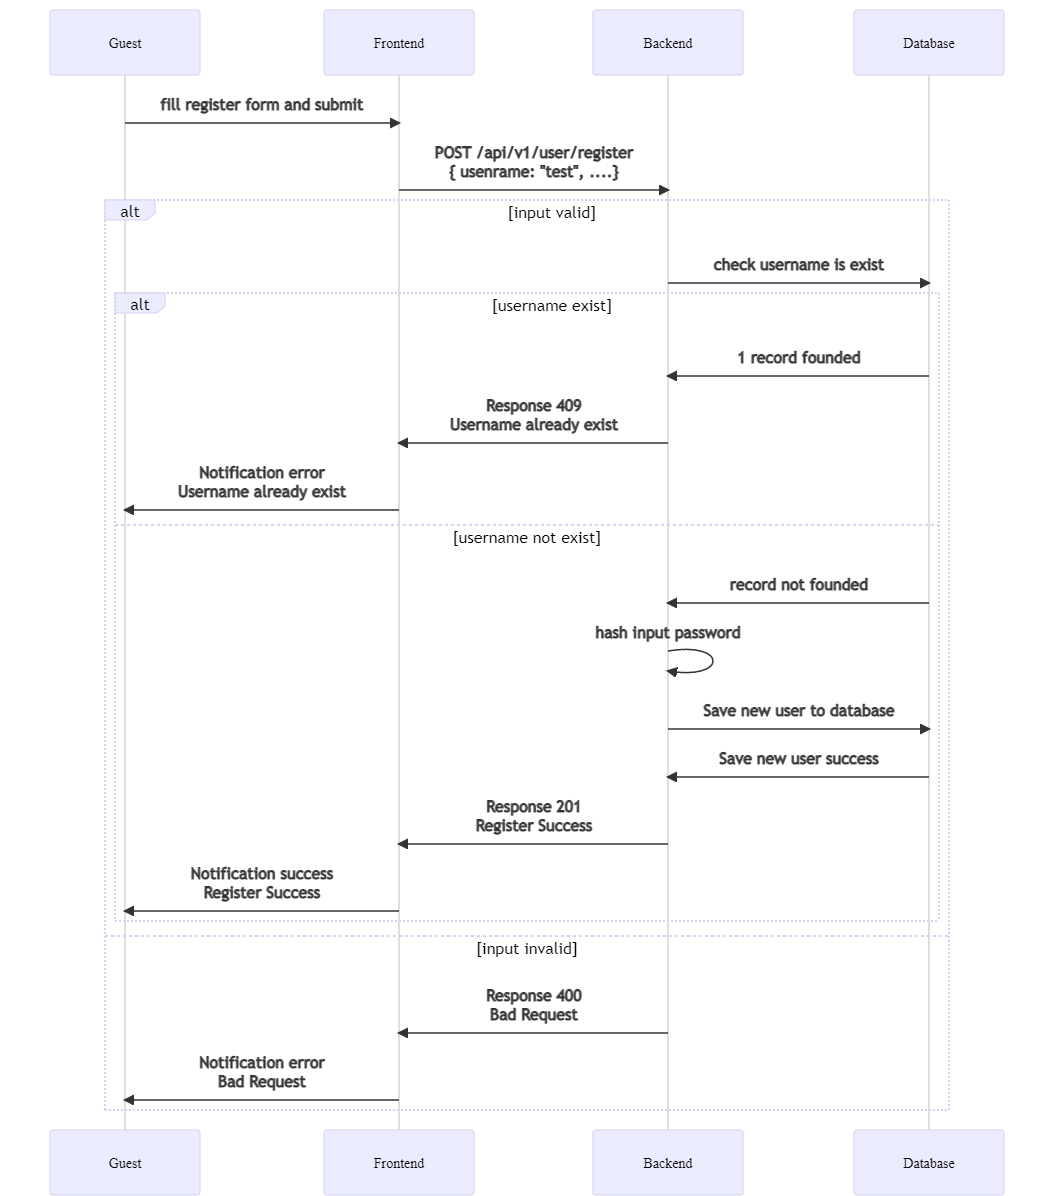
\includegraphics[width=\textwidth]{./img/seq_regis.png}
  \caption{Sequence diagram ของการสมัครสมาชิก}\label{fig:seq_regis} 
\end{figure}
\newpage
\begin{longtable}[!ht]{p{3cm}|p{8cm}}
  \caption{API Document ของ User ในการสร้างบัญชีสำหรับใช้งานภายในระบบ}\label{tbl:api_user_regis} 
  \endfirsthead
  \endhead
  \hhline{==}
  \textbf{URL}              & /api/v1/user/register                                                                                               \\ \hline
  \textbf{Description}      & สร้างบัญชีสำหรับใช้งานภายในระบบ                                                                                          \\ \hline
  \textbf{METHOD}           & POST                                                                                                                \\ \hline
  \textbf{HEADER}           & -                                                                                                                   \\ \hline
  \textbf{PAYLOAD}          & \begin{tabular}[c]{@{}l@{}}email:\quad string\\ password:\quad string\\ firstName:\quad string\\ lastname:\quad string \\ image:\quad file\end{tabular}  \\ \hline  \hline
  \textbf{Response Status}  & \multicolumn{1}{c}{\textbf{Response Data}}                                                                          \\ \hline
  \multicolumn{1}{c|}{201}  & \begin{tabular}[c]{@{}l@{}}\{\\ \quad message: "register successfull"\\ \}\end{tabular}                                 \\ \hline
  \multicolumn{1}{c|}{409}  &
  \begin{tabular}[c]{@{}l@{}}\{\\ \quad errors: {[}\\ \quad\quad\{\\ \quad\quad\quad "message": "Email already exist"\\ \quad\quad \}\\ \quad{]}\\\}\end{tabular} \\ \hline
  \multicolumn{1}{c|}{400}  &
  \begin{tabular}[c]{@{}l@{}}\{\\ \quad errors: {[}\\ \quad\quad\{\\ \quad\quad\quad "field": "Email",\\ \quad\quad\quad"message": "This field is required"\\ \quad\quad\},\\ 
    \quad\quad\{\\ \quad\quad\quad"field": "password",\\ \quad\quad\quad "message": "This field is required"\\ \quad\quad \}\\\quad {]}\\ \}\end{tabular}                                                                         \\ \hline
  \hhline{==}
\end{longtable}

\subsubsection{ผู้ใช้งานเข้าสู่ระบบ}
\textbf{Name: }ผู้ใช้งานเข้าสู่ระบบ \\
\textbf{Actors: }ผู้ใช้งานทั่วไป \\
\textbf{Goal: }ผู้ใช้งานสามารถเข้าสู่ระบบได้ \\
\textbf{Precondition: }ผู้ใช้งานสมัครสมาชิกแล้ว \\
\textbf{Main success scenario: } \\
  \hspace*{0.5cm}1. ผู้ใช้งานกรอก Email และ Password \\
  \hspace*{0.5cm}2. ผู้ใช้งานส่งคำร้องขอเข้าสู่ระบบ \\
  \hspace*{0.5cm}3. ระบบตรวจสอบ Email และ Password ตรงกับในฐานข้อมูล \\
  \hspace*{0.5cm}4. ผู้ใช้งานสามารถเข้าสู่ระบบได้ \\ \newpage
\textbf{Extension (a): } \\ 
  \hspace*{0.5cm}3a. ระบบตรวจสอบข้อมูลพบว่าผู้ใช้งานกรอกข้อมูลไม่ครบ \\
  \hspace*{0.5cm}4a. ผู้ใช้งานได้รับแจ้งเตือนว่ากรอกข้อมูลไม่ครบ \\
  \hspace*{0.5cm}5a. กลับไปที่ข้อที่ 1 \\
\textbf{Extension (b): }  \\
  \hspace*{0.5cm}3a. ระบบตรวจสอบข้อมูลพบว่าไม่มี Email และ Password ตรงกับในฐานข้อมูล \\
  \hspace*{0.5cm}4a. ผู้ใช้งานได้รับแจ้งเตือนว่า Email และ Password ไม่ถูกต้อง \\
  \hspace*{0.5cm}5a. กลับไปที่ข้อที่ 1 
\begin{figure}[!ht]\centering
  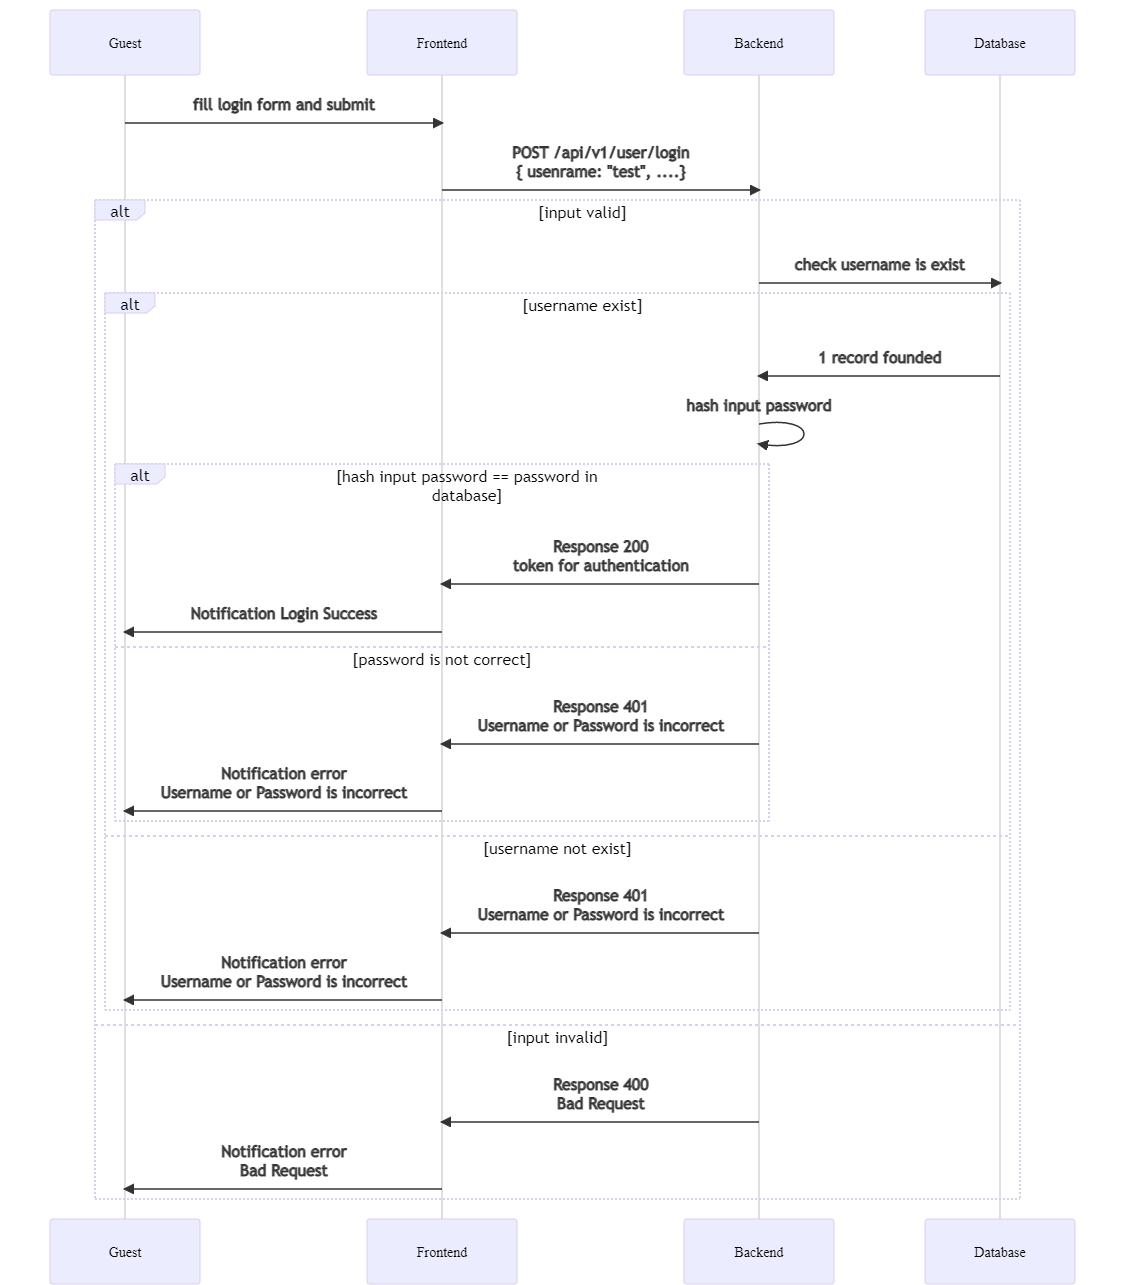
\includegraphics[width=\textwidth]{./img/seq_login.png}
  \caption{Sequence diagram ของการเข้าสู่ระบบ}\label{fig:seq_login} 
\end{figure} 
\begin{longtable}[!ht]{p{3cm}|p{8cm}}
  \caption{API Document ของ User ในการเข้าสู่ระบบบัญชีผู้ใช้งาน}\label{tbl:api_user_login} 
  \endfirsthead
  \endhead
  \hhline{==}
  \textbf{URL}              & /api/v1/user/login                                                                                                   \\ \hline
  \textbf{Description}      & เข้าสู่ระบบบัญชีผู้ใช้งาน                                                                                                   \\ \hline
  \textbf{METHOD}           & POST                                                                                                                \\ \hline
  \textbf{HEADER}           & -                                                                                                                   \\ \hline
  \textbf{PAYLOAD}          & \begin{tabular}[c]{@{}l@{}}email:\quad string\\ password:\quad string\end{tabular}                               \\ \hline \hline
  \textbf{Response Status}  & \multicolumn{1}{c}{\textbf{Response Data}}                                                                          \\ \hline
  \multicolumn{1}{c|}{200}  & \begin{tabular}[c]{@{}l@{}}\{\\ \quad message: "login successfull",\\ \quad token: "xxxxxxxxxxxxxx" \\\}\end{tabular}                                 \\ \hline
  \multicolumn{1}{c|}{400}  &
  \begin{tabular}[c]{@{}l@{}}\{\\ \quad errors: {[}\\ \quad\quad\{\\ \quad\quad\quad "message": "Email or password is invalid"\\ \quad\quad \}\\ \quad{]}\\\}\end{tabular}                                                                      \\ \hline
  \hline
\end{longtable}

\subsubsection{ตรวจสอบข้อมูลโปรไฟล์ของตนเอง}
\textbf{Name: }สมาชิกตรวจสอบข้อมูลโปรไฟล์ของตนเอง \\
\textbf{Actors: }สมาชิก (ผู้ใช้งานที่ลงทะเบียนแล้ว) \\
\textbf{Goal: }สมาชิกสามารถเรียกดูข้อมูลโปรไฟล์ของตนเองได้ \\
\textbf{Precondition: }สมาชิกต้องทำการเข้าสู่ระบบแล้ว \\
\textbf{Main success scenario: } \\
  \hspace*{0.5cm}1. สมาชิกร้องขอดูข้อมูลโปรไฟล์ของตนเอง  \\
  \hspace*{0.5cm}2. ระบบดึงข้อมูลโปรไฟล์แสดงผลให้สมาชิก \\ \newpage 
\begin{figure}[!ht]\centering
  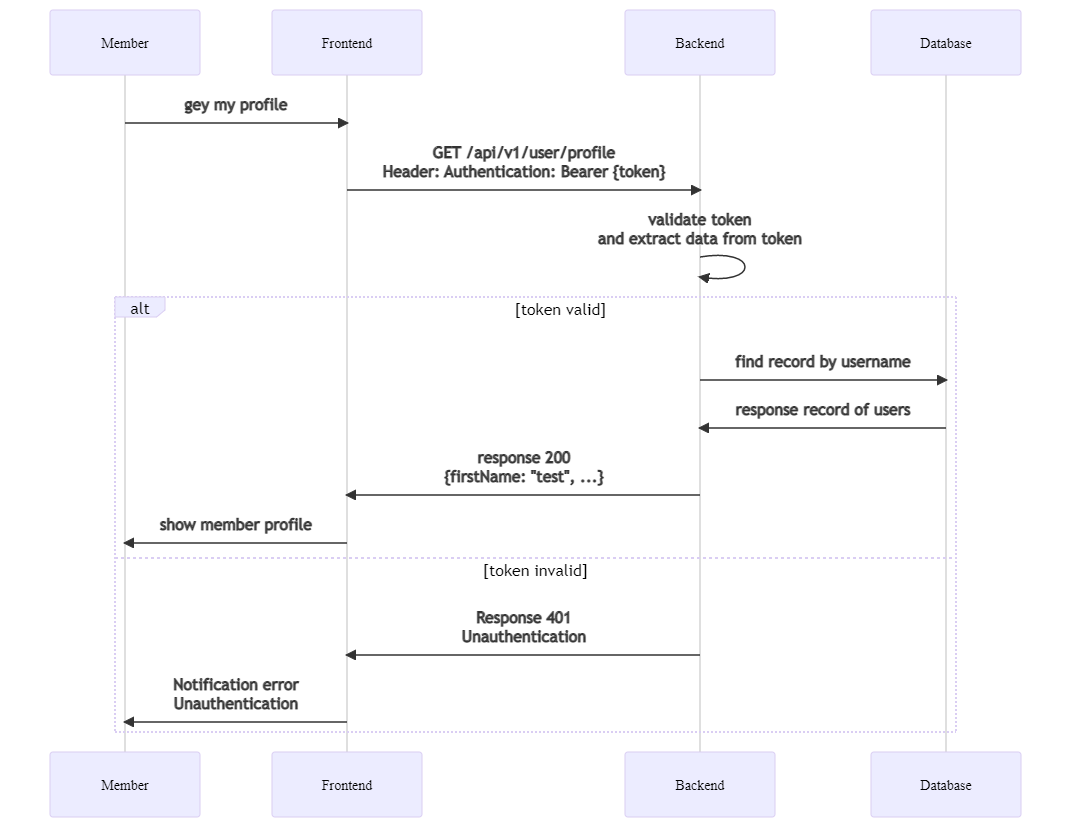
\includegraphics[width=\textwidth]{./img/seq_profile.png}
  \caption{Sequence diagram ของการตรวจสอบข้อมูลโปรไฟล์}\label{fig:seq_profile} 
\end{figure} 
\begin{longtable}[!ht]{p{3cm}|p{8cm}}
  \caption{API Document ของ User ในการดูรายละเอียดโปรไฟล์ของตนเอง}\label{tbl:api_user_profile} 
    \endfirsthead
    \endhead
    \hhline{==}
    \textbf{URL}              & /api/v1/user/profile                                                                                               \\ \hline
    \textbf{Description}      & ดูรายละเอียดโปรไฟล์ของตนเอง                                                                                            \\ \hline
    \textbf{METHOD}           & GET                                                                                                                 \\ \hline
    \textbf{HEADER}           & Authorization: Bearer \{token\}                                                                                       \\ \hline 
    \textbf{PAYLOAD}          & -                                                                                                                   \\ \hline \newpage \hline 
    \textbf{Response Status}  & \multicolumn{1}{c}{\textbf{Response Data}}                                                                          \\ \hline
    \multicolumn{1}{c|}{200}  & \begin{tabular}[c]{@{}l@{}}\{\\ \quad id: "1",\\ \quad firstName: "Ponlawat",\\ \quad lastName: "Suparat" \\
      \quad email: ""test@gmail.com"",\\ \quad role: "Member",\\ \quad api\_key: "asdasfwaefdfaxcvasdv324234"\\\}\end{tabular}           \\ \hline
    \multicolumn{1}{c|}{401}  &
    \begin{tabular}[c]{@{}l@{}}\{\\ \quad errors: {[}\\ \quad\quad\{\\ \quad\quad\quad "message": "Unauthorization"\\ \quad\quad \}\\ \quad{]}\\\}\end{tabular}                                                                         \\ \hline
    \hhline{==}
\end{longtable}

\subsubsection{สร้างคำร้องขอวิเคราะห์หมวดหมู่ของเนื้อหาด้วย Web Link}
\textbf{Name: }สมาชิกสร้างคำร้องขอวิเคราะห์หมวดหมู่ของเนื้อหาด้วย Web Link \\
\textbf{Actors: }สมาชิก (ผู้ใช้งานที่ลงทะเบียนแล้ว) \\
\textbf{Goal: }สมาชิกส่งคำร้องขอวิเคราะห์หมวดหมู่ของเนื้อหาไปยังระบบสำเร็จ \\
\textbf{Precondition: }สมาชิกต้องทำการเข้าสู่ระบบแล้ว \\
\textbf{Main success scenario: } \\
  \hspace*{0.5cm}1. สมาชิกกรอกแบบฟอร์ม รวมไปถึงกรอก Web Link ที่ต้องการวิเคราะห์หมวดหมู่ของเนื้อหา \\
  \hspace*{0.5cm}2. สมาชิกส่งแบบฟอร์มมายังระบบ \\
  \hspace*{0.5cm}3. ระบบทำการตอบกลับด้วยเลขคำร้องขอ \\
  \hspace*{0.5cm}4. ระบบประมวลผลเสร็จสิ้นและส่งการแจ้งเตือนกลับไปยังสมาชิก \\
\textbf{Extension (a): } \\
  \hspace*{0.5cm}3a. ระบบตรวจสอบข้อมูลพบว่าสมาชิกกรอกข้อมูลไม่ครบ \\
  \hspace*{0.5cm}4a. สมาชิกได้รับแจ้งเตือนว่ากรอกข้อมูลไม่ครบ \\
  \hspace*{0.5cm}5a. กลับไปที่ข้อที่ 1 \newpage
\begin{figure}[!ht]\centering
  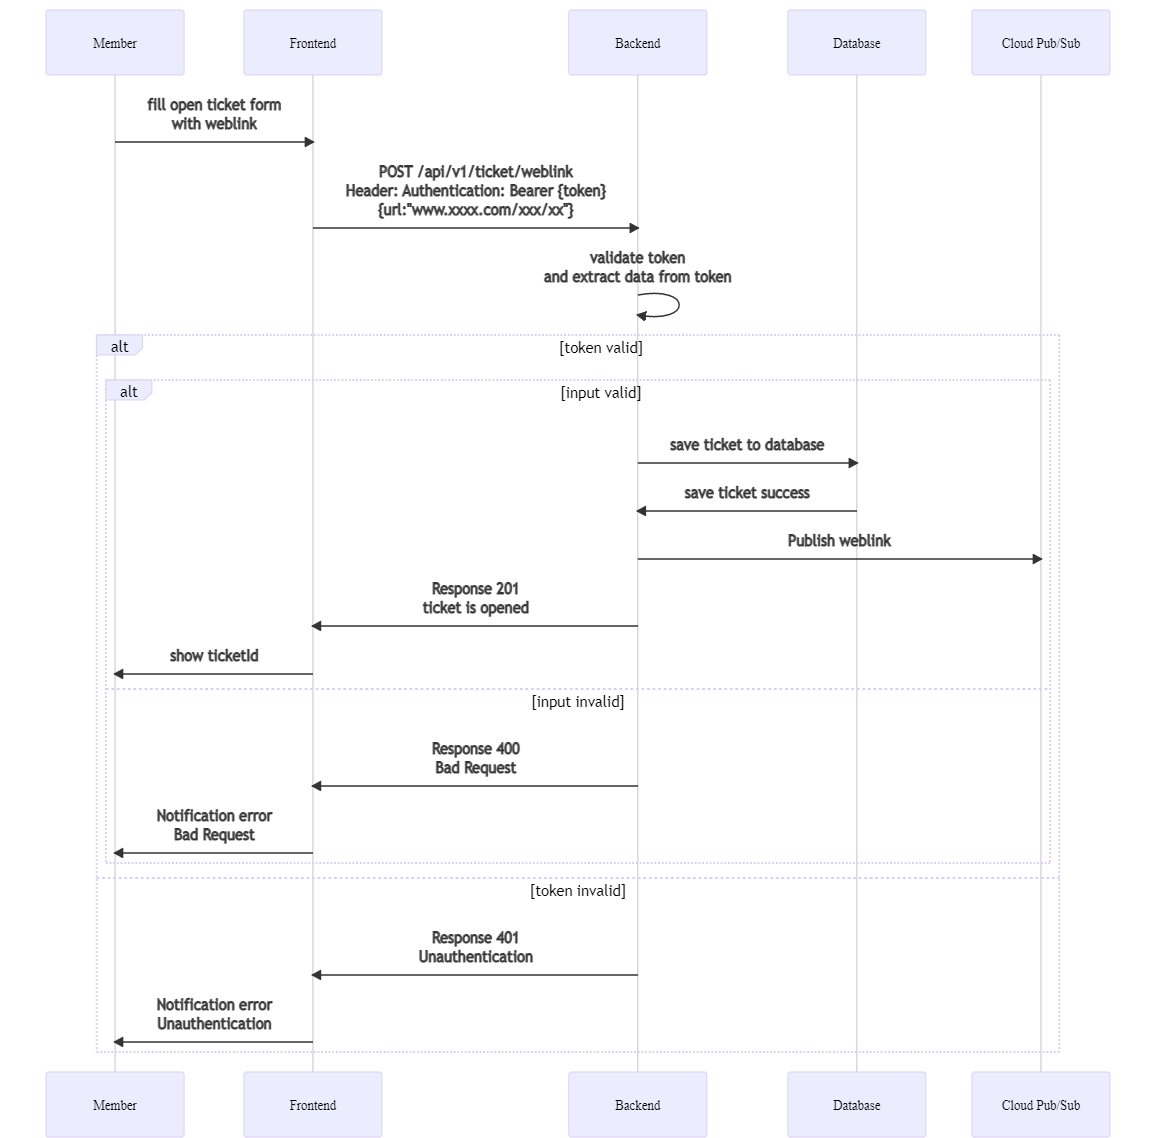
\includegraphics[width=\textwidth]{./img/seq_weblink.png}
  \caption{Sequence diagram ของการสร้างคำร้องขอวิเคราะห์หมวดหมู่ของเนื้อหาด้วย Web Link}\label{fig:seq_weblink} 
\end{figure} 
\begin{longtable}[!ht]{p{3cm}|p{8cm}}
  \caption{API Document ของ Ticket ในการสร้างคำร้องขอวิเคราะห์หมวดหมู่ของเนื้อหาด้วย Web Link}\label{tbl:api_ticket_weblink} 
    \endfirsthead
    \endhead
    \hhline{==}
    \textbf{URL}              & /api/v1/ticket/weblink/                                                                                              \\ \hline
    \textbf{Description}      & สร้างคำร้องขอวิเคราะห์หมวดหมู่ของเนื้อหาด้วย Web Link                                                                                        \\ \hline
    \textbf{METHOD}           & POST                                                                                                                 \\ \hline
    \textbf{HEADER}           & Authorization: Bearer \{token\}                                                                                         \\ \hline
    \textbf{PAYLOAD}          & \begin{tabular}[c]{@{}l@{}}url: string\end{tabular}  \\ \hline \newpage \hline
    \textbf{Response Status}  & \multicolumn{1}{c}{\textbf{Response Data}}                                                                          \\ \hline
    \multicolumn{1}{c|}{201}  & \begin{tabular}[c]{@{}l@{}}\{\\ \quad ticketId: 123,\\ \quad status: "Open"\\ \}\end{tabular}                                 \\ \hline
    \multicolumn{1}{c|}{400}  &
    \begin{tabular}[c]{@{}l@{}}\{\\ \quad errors: {[}\\ \quad\quad\{\\ \quad\quad\quad "field": "url"\\ \quad\quad\quad "message": "This field is required"\\ \quad\quad \}\\ \quad{]}\\\}\end{tabular} \\ \hline
    \multicolumn{1}{c|}{401}  &
    \begin{tabular}[c]{@{}l@{}}\{\\ \quad errors: {[}\\ \quad\quad\{\\ \quad\quad\quad"message": "Unauthorization"\\ \quad\quad\}\\\quad {]}\\ \}\end{tabular}                                                                         \\ \hline
    \hhline{==}
\end{longtable}

\subsubsection{สร้างคำร้องขอวิเคราะห์หมวดหมู่ของเนื้อหาด้วยบทความ}
\textbf{Name: }สมาชิกสร้างคำร้องขอวิเคราะห์หมวดหมู่ของเนื้อหาด้วยบทความ \\
\textbf{Actors: }สมาชิก (ผู้ใช้งานที่ลงทะเบียนแล้ว) \\
\textbf{Goal: }สมาชิกส่งคำร้องขอวิเคราะห์หมวดหมู่ของเนื้อหาไปยังระบบสำเร็จ \\
\textbf{Precondition: }สมาชิกต้องทำการเข้าสู่ระบบแล้ว \\
\textbf{Main success scenario: } \\
  \hspace*{0.5cm}1. สมาชิกกรอกแบบฟอร์ม รวมไปถึงกรอกบทความที่ต้องการวิเคราะห์หมวดหมู่ของเนื้อหา \\
  \hspace*{0.5cm}2. สมาชิกส่งแบบฟอร์มมายังระบบ \\
  \hspace*{0.5cm}3. ระบบทำการตอบกลับด้วยเลขคำร้องขอ \\
  \hspace*{0.5cm}4. ระบบประมวลผลเสร็จสิ้นและส่งการแจ้งเตือนกลับไปยังสมาชิก \\
\textbf{Extension (a): } \\
  \hspace*{0.5cm}3a. ระบบตรวจสอบข้อมูลพบว่าสมาชิกกรอกข้อมูลไม่ครบ \\
  \hspace*{0.5cm}4a. สมาชิกได้รับแจ้งเตือนว่ากรอกข้อมูลไม่ครบ \\
  \hspace*{0.5cm}5a. กลับไปที่ข้อที่ 1 \newpage
\begin{figure}[!ht]\centering
  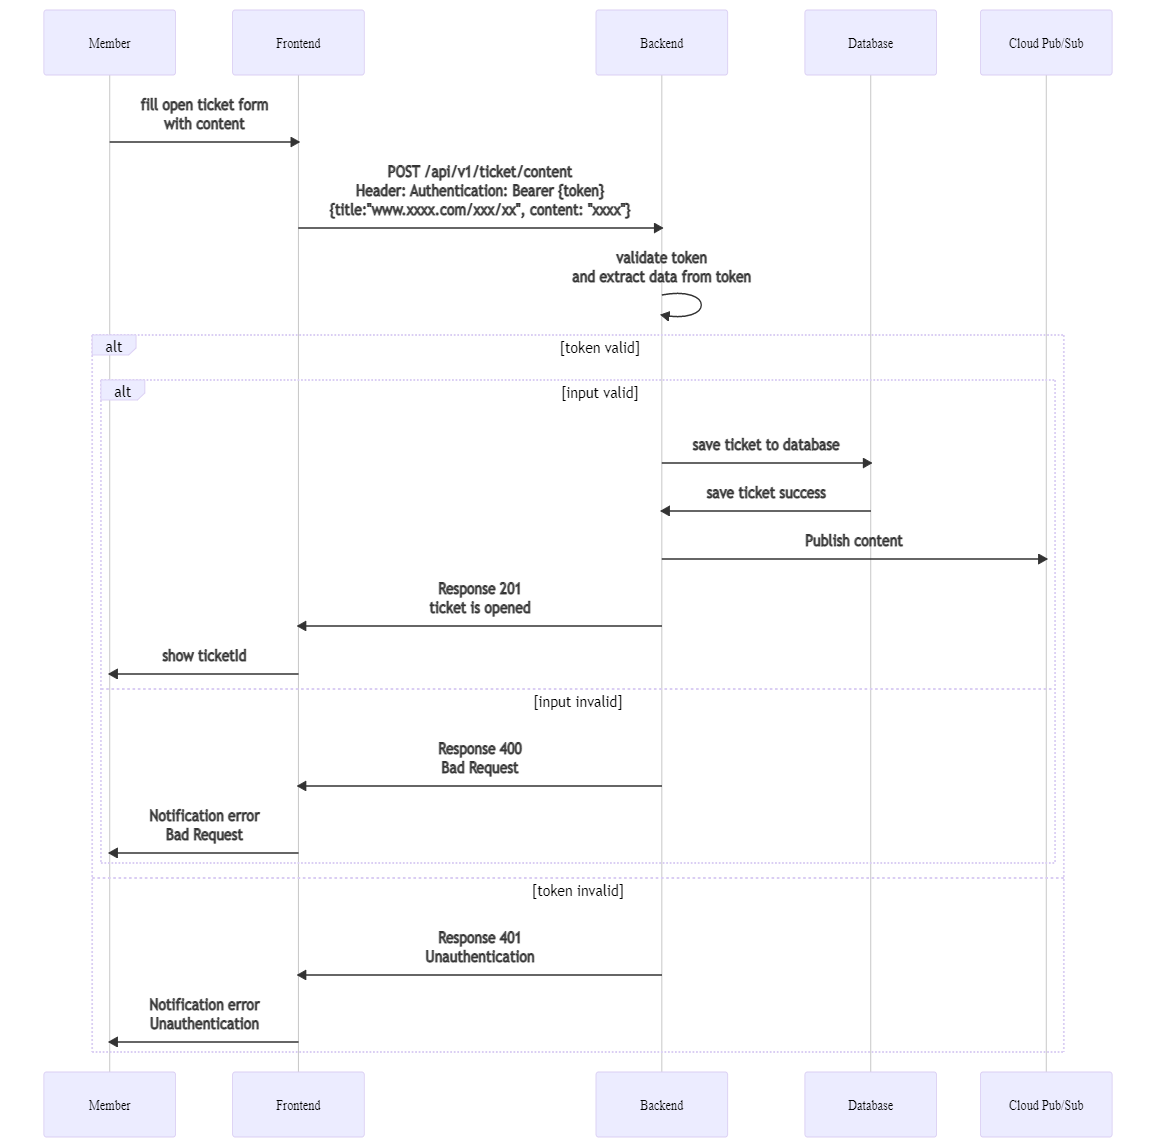
\includegraphics[width=\textwidth]{./img/seq_content.png}
  \caption{Sequence diagram ของการสร้างคำร้องขอวิเคราะห์หมวดหมู่ของเนื้อหาด้วยบทความ}\label{fig:seq_content} 
\end{figure} 
\begin{longtable}[!ht]{p{3cm}|p{8cm}}
  \caption{API Document ของ Ticket ในการสร้างคำร้องขอวิเคราะห์ด้วยเนื้อหาที่เตรียมไว้ }\label{tbl:api_ticket_content} 
    \endfirsthead
    \endhead
    \hhline{==}
    \textbf{URL}              & /api/v1/ticket/content/                                                                                              \\ \hline
    \textbf{Description}      & สร้างคำร้องขอวิเคราะห์ด้วยเนื้อหาที่เตรียมไว้                                                                                      \\ \hline
    \textbf{METHOD}           & POST                                                                                                                 \\ \hline
    \textbf{HEADER}           & Authorization: Bearer \{token\}                                                                                         \\ \hline
    \textbf{PAYLOAD}          & \begin{tabular}[c]{@{}l@{}}title:\quad\quad string \\ content:\quad string\end{tabular}  \\ \hline \newpage \hline
    \textbf{Response Status}  & \multicolumn{1}{c}{\textbf{Response Data}}                                                                          \\ \hline
    \multicolumn{1}{c|}{201}  & \begin{tabular}[c]{@{}l@{}}\{\\ \quad ticketId: 123,\\ \quad status: "Open"\\ \}\end{tabular}                                 \\ \hline
    \multicolumn{1}{c|}{400}  &
    \begin{tabular}[c]{@{}l@{}}\{\\ \quad errors: {[}\\ \quad\quad\{\\ \quad\quad\quad "field": "title",\\ \quad\quad\quad"message": "This field is required"\\ \quad\quad\},\\ 
      \quad\quad\{\\ \quad\quad\quad"field": "content",\\ \quad\quad\quad "message": "This field is required"\\ \quad\quad \}\\\quad {]}\\ \}\end{tabular}  \\ \hline
    \multicolumn{1}{c|}{401}  &
    \begin{tabular}[c]{@{}l@{}}\{\\ \quad errors: {[}\\ \quad\quad\{\\ \quad\quad\quad"message": "Unauthorization"\\ \quad\quad\}\\\quad {]}\\ \}\end{tabular}                                                                         \\ \hline
    \hhline{==}
\end{longtable}

\subsubsection{สร้างคำร้องขอวิเคราะห์หมวดหมู่ของเนื้อหาด้วย Web Link ผ่าน Api-Key}
\textbf{Name: }สมาชิกสร้างคำร้องขอวิเคราะห์หมวดหมู่ของเนื้อหาด้วย Web Link ผ่าน Api-Key \\
\textbf{Actors: }สมาชิก (ผู้ใช้งานที่ลงทะเบียนแล้ว) \\
\textbf{Goal: }สมาชิกส่งคำร้องขอวิเคราะห์หมวดหมู่ของเนื้อหาไปยังระบบสำเร็จ \\
\textbf{Precondition: }สมาชิกต้องทำการสร้าง Api-Key และลงทะเบียน Web Hook สำหรับรับข้อมูลการประมวลผล \\
\textbf{Main success scenario: } \\
  \hspace*{0.5cm}1. สมาชิกส่งคำร้องขอวิเคราะห์หมวดหมู่ของเนื้อหาด้วย Web Link มายังระบบ พร้อมกับ Api-Key \\
  \hspace*{0.5cm}2. ระบบทำการตอบกลับด้วยเลขคำร้องขอ \\
  \hspace*{0.5cm}3. ระบบประมวลผลเสร็จสิ้นและส่งการแจ้งเตือนกลับไปยังสมาชิกผ่าน Web Hook Url  \\
\textbf{Extension (a): } \\
  \hspace*{0.5cm}2a. ระบบตรวจสอบข้อมูลพบว่าสมาชิกส่งข้อมูลไม่ครบ \\
  \hspace*{0.5cm}3a. สมาชิกได้รับแจ้งเตือนว่าส่งข้อมูลไม่ครบ \\
  \hspace*{0.5cm}4a. กลับไปที่ข้อที่ 1 \newpage
\begin{figure}[!ht]\centering
  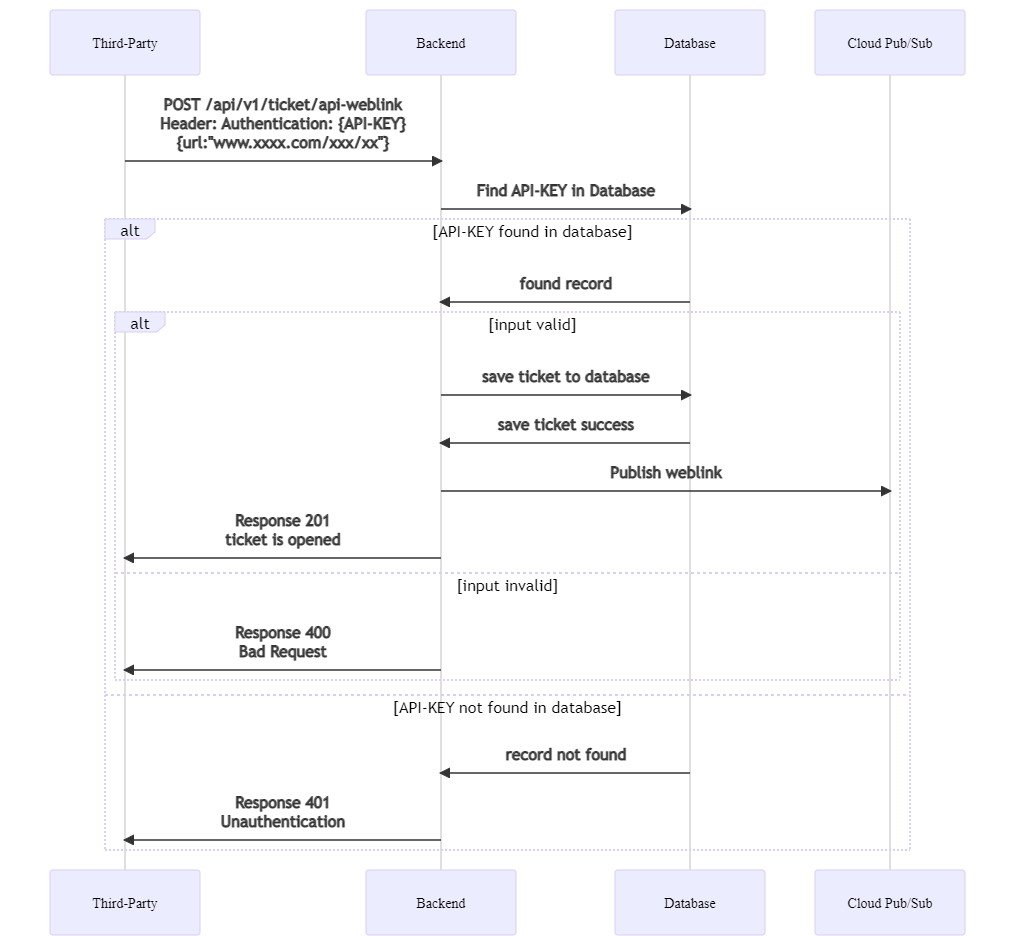
\includegraphics[width=\textwidth]{./img/seq_linkapi.png}
  \caption{Sequence diagram ของการสร้างคำร้องขอวิเคราะห์หมวดหมู่ของเนื้อหาด้วย Web Link ผ่าน Api-Key}\label{fig:seq_weblink_api} 
\end{figure} 
\begin{longtable}[!ht]{p{3cm}|p{8cm}}
  \caption{API Document ของ Ticket ในการสร้างคำร้องขอวิเคราะห์ด้วย Web Link (Api-key)}\label{tbl:api_ticket_key} 
    \endfirsthead
    \endhead
    \hhline{==}  
    \textbf{URL}              & /api/v1/ticket/api-weblink/                                                                                            \\ \hline
    \textbf{Description}      & สร้างคำร้องขอวิเคราะห์ด้วย Web Link (Api-key)                                                                                     \\ \hline
    \textbf{METHOD}           & POST                                                                                                                 \\ \hline
    \textbf{HEADER}           & Authorization: \{api-key\}                                                                                         \\ \hline
    \textbf{PAYLOAD}          & \begin{tabular}[c]{@{}l@{}}url: string\end{tabular}  \\ \hline \newpage \hline
    \textbf{Response Status}  & \multicolumn{1}{c}{\textbf{Response Data}}                                                                          \\ \hline
    \multicolumn{1}{c|}{201}  & \begin{tabular}[c]{@{}l@{}}\{\\ \quad ticketId: 123,\\ \quad status: "Open"\\ \}\end{tabular}                                 \\ \hline
    \multicolumn{1}{c|}{400}  &
    \begin{tabular}[c]{@{}l@{}}\{\\ \quad errors: {[}\\ \quad\quad\{\\ \quad\quad\quad "field": "url"\\ \quad\quad\quad "message": "This field is required"\\ \quad\quad \}\\ \quad{]}\\\}\end{tabular} \\ \hline
    \multicolumn{1}{c|}{401}  &
    \begin{tabular}[c]{@{}l@{}}\{\\ \quad errors: {[}\\ \quad\quad\{\\ \quad\quad\quad"message": "Unauthorization"\\ \quad\quad\}\\\quad {]}\\ \}\end{tabular}                                                                         \\ \hline
    \hhline{==}  
\end{longtable}

\subsubsection{สร้างคำร้องขอวิเคราะห์หมวดหมู่ของเนื้อหาด้วยบทความผ่าน Api-Key}
\textbf{Name: }สมาชิกสร้างคำร้องขอวิเคราะห์หมวดหมู่ของเนื้อหาด้วยบทความผ่าน Api-Key \\
\textbf{Actors: }สมาชิก (ผู้ใช้งานที่ลงทะเบียนแล้ว) \\
\textbf{Goal: }สมาชิกส่งคำร้องขอวิเคราะห์หมวดหมู่ของเนื้อหาไปยังระบบสำเร็จ \\
\textbf{Precondition: }สมาชิกต้องทำการสร้าง Api-Key และลงทะเบียน Web Hook สำหรับรับข้อมูลการประมวลผล \\
\textbf{Main success scenario: } \\
  \hspace*{0.5cm}1. สมาชิกส่งคำร้องขอวิเคราะห์หมวดหมู่ของเนื้อหาด้วยบทความมายังระบบ พร้อมกับ Api-Key \\
  \hspace*{0.5cm}2. ระบบทำการตอบกลับด้วยเลขคำร้องขอ \\
  \hspace*{0.5cm}3. ระบบประมวลผลเสร็จสิ้นและส่งการแจ้งเตือนกลับไปยังสมาชิกผ่าน Web Hook Url  \\
\textbf{Extension (a): } \\
  \hspace*{0.5cm}2a. ระบบตรวจสอบข้อมูลพบว่าสมาชิกส่งข้อมูลไม่ครบ \\
  \hspace*{0.5cm}3a. สมาชิกได้รับแจ้งเตือนว่าส่งข้อมูลไม่ครบ \\
  \hspace*{0.5cm}4a. กลับไปที่ข้อที่ 1 \newpage
\begin{figure}[!ht]\centering
  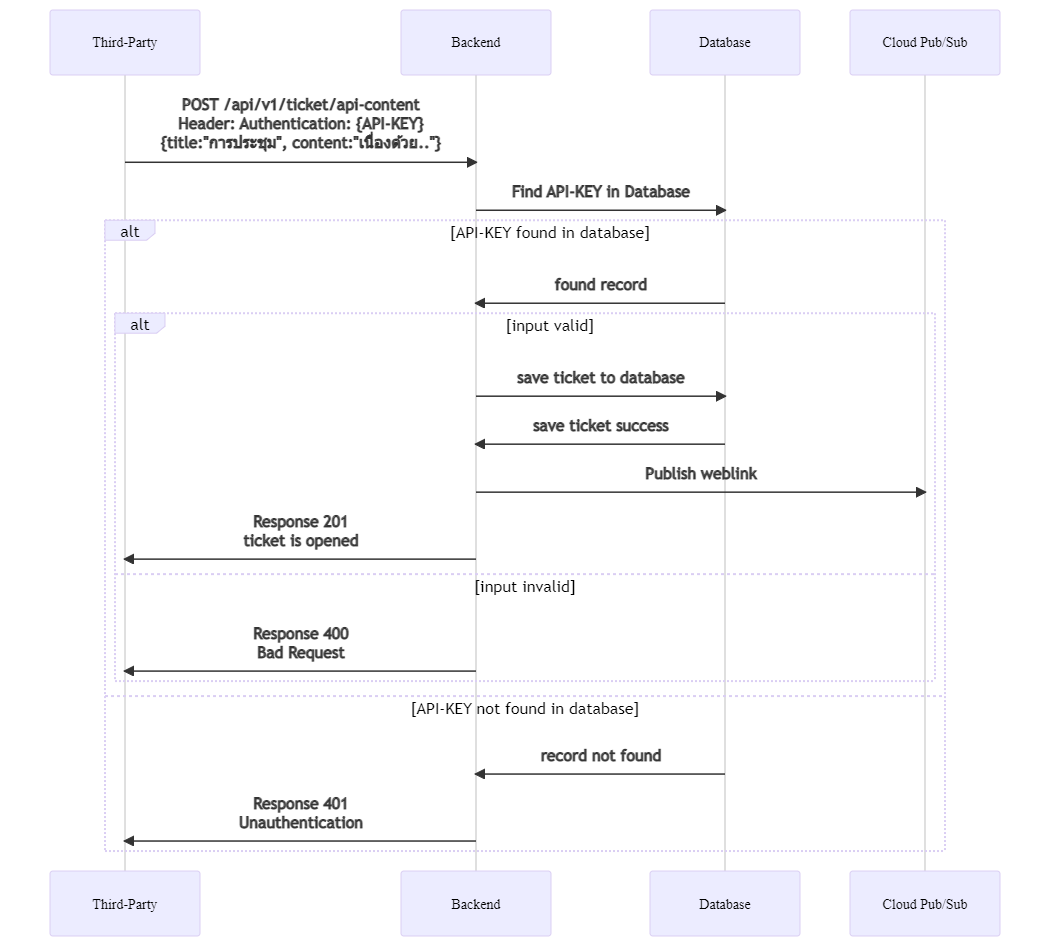
\includegraphics[width=\textwidth]{./img/seq_contapi.png}
  \caption{Sequence diagram ของการสร้างคำร้องขอวิเคราะห์หมวดหมู่ของเนื้อหาด้วยบทความผ่าน Api-Key}\label{fig:seq_content_api} 
\end{figure}
\begin{longtable}[!ht]{p{3cm}|p{8cm}}
  \caption{API Document ของ Ticket ในการสร้างคำร้องขอวิเคราะห์ด้วยเนื้อหาที่เตรียมไว้ (Api-Key) }\label{tbl:api_ticket_content_key} 
    \endfirsthead
    \endhead
    \hhline{==} 
    \textbf{URL}              & /api/v1/ticket/api-content/                                                                                            \\ \hline
    \textbf{Description}      & สร้างคำร้องขอวิเคราะห์ด้วยเนื้อหาที่เตรียมไว้ (Api-Key)                                                                                     \\ \hline
    \textbf{METHOD}           & POST                                                                                                                 \\ \hline
    \textbf{HEADER}           & Authorization: \{Api-Key\}                                                                                         \\ \hline
    \textbf{PAYLOAD}          & \begin{tabular}[c]{@{}l@{}}title:\quad\quad string \\ content:\quad string\end{tabular}  \\ \hline \newpage \hline
    \textbf{Response Status}  & \multicolumn{1}{c}{\textbf{Response Data}}                                                                          \\ \hline
    \multicolumn{1}{c|}{201}  & \begin{tabular}[c]{@{}l@{}}\{\\ \quad ticketId: 123,\\ \quad status: "Open"\\ \}\end{tabular}                                 \\ \hline
    \multicolumn{1}{c|}{400}  &
    \begin{tabular}[c]{@{}l@{}}\{\\ \quad errors: {[}\\ \quad\quad\{\\ \quad\quad\quad "field": "title",\\ \quad\quad\quad"message": "This field is required"\\ \quad\quad\},\\ 
      \quad\quad\{\\ \quad\quad\quad"field": "content",\\ \quad\quad\quad "message": "This field is required"\\ \quad\quad \}\\\quad {]}\\ \}\end{tabular}  \\ \hline
    \multicolumn{1}{c|}{401}  &
    \begin{tabular}[c]{@{}l@{}}\{\\ \quad errors: {[}\\ \quad\quad\{\\ \quad\quad\quad"message": "Unauthorization"\\ \quad\quad\}\\\quad {]}\\ \}\end{tabular}                                                                         \\ \hline
    \hhline{==} 
\end{longtable}

\subsubsection{ดูคำร้องขอการวิเคราะห์หมู่ของบทความของตนเอง}
\textbf{Name: }สมาชิกดูคำร้องขอการวิเคราะห์หมู่ของบทความของตนเอง \\
\textbf{Actors: }สมาชิก (ผู้ใช้งานที่ลงทะเบียนแล้ว) \\
\textbf{Goal: }สมาชิกส่งคำร้องขอการวิเคราะห์หมู่ของบทความไปยังระบบสำเร็จ \\
\textbf{Precondition: }สมาชิกต้องทำการเข้าสู่ระบบแล้ว \\
\textbf{Main success scenario: } \\
  \hspace*{0.5cm}1. สมาชิกร้องขอดูข้อมูลคำร้องของตนเอง  \\
  \hspace*{0.5cm}2. ระบบดึงข้อมูลคำร้องของสมาชิกและแสดงผลให้สมาชิก \\ \newpage
\begin{figure}[!ht]\centering
  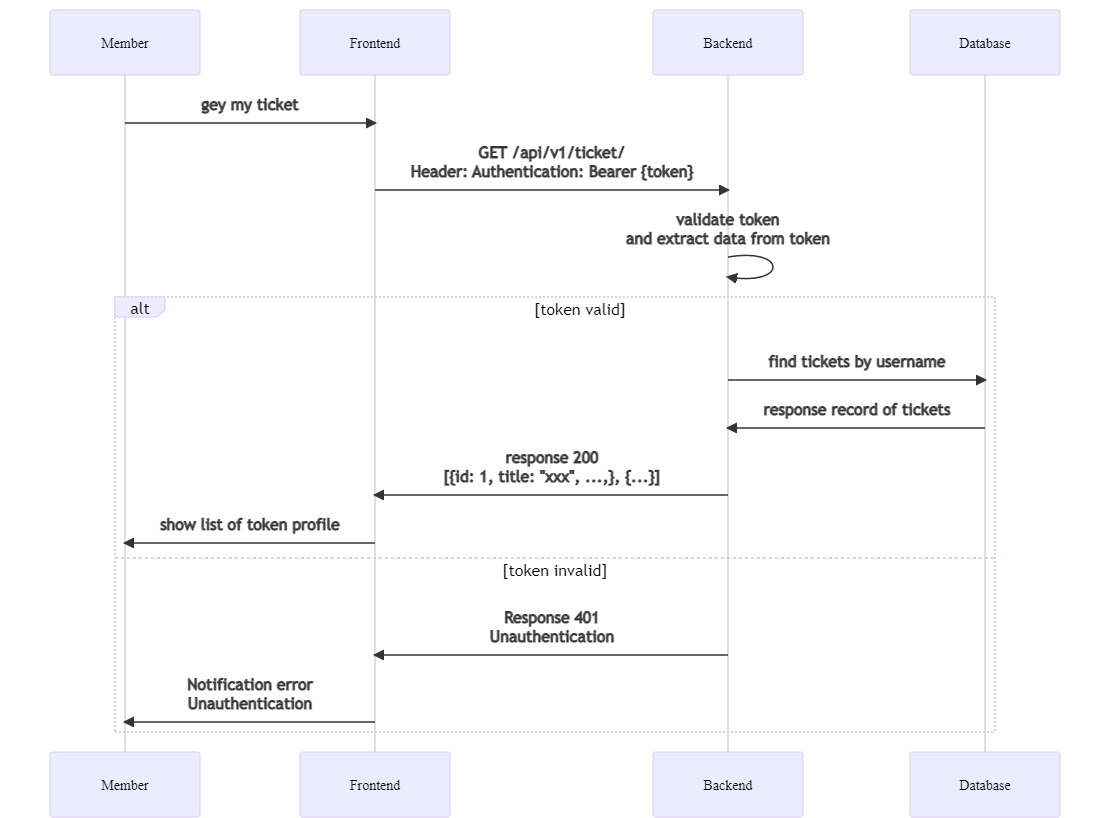
\includegraphics[width=\textwidth]{./img/seq_request.png}
  \caption{Sequence diagram ของการดูคำร้องขอการวิเคราะห์หมู่ของบทความ}\label{fig:seq_request} 
\end{figure} 
\begin{longtable}[!ht]{p{3cm}|p{8cm}}
  \caption{API Document ของ Ticket ในการดูรายการคำร้องขอของตนเอง}\label{tbl:api_ticket} 
    \endfirsthead
    \endhead
    \hhline{==}  
    \textbf{URL}              & /api/v1/ticket/                                                                                             \\ \hline
    \textbf{Description}      & ดูรายการคำร้องขอของตนเอง                                                                                     \\ \hline
    \textbf{METHOD}           & GET                                                                                                                 \\ \hline
    \textbf{HEADER}           & Authorization: Bearer \{token\}                                                                                         \\ \hline
    \textbf{PAYLOAD}          &   \\ \hline \newpage \hline
    \textbf{Response Status}  & \multicolumn{1}{c}{\textbf{Response Data}}                                                                          \\ \hline
    \multicolumn{1}{c|}{200}  &
    \begin{tabular}[c]{@{}l@{}}{[}\\ \quad\{\\ \quad\quad id: 1,\\ \quad\quad title: "การประชุม...",\\\quad\quad status: "processing",\\ 
      \quad\quad category: {[}{]},\\ \quad\quad detial: "www.ai-tagging.com/content/1"\\ \quad\},\\ 
      \quad\{\\ \quad\quad id: 2,\\ \quad\quad title: "ดาราหนุ่มเตะฟุตบอล",\\\quad\quad status: "succcess",\\ 
      \quad\quad category: {[}"บันเทิง", "กีฬา"{]},\\ \quad\quad detial: "www.ai-tagging.com/content/2"\\ \quad \}\\{]}\end{tabular}  \\ \hline
    \multicolumn{1}{c|}{401}  &
    \begin{tabular}[c]{@{}l@{}}\{\\ \quad errors: {[}\\ \quad\quad\{\\ \quad\quad\quad"message": "Unauthorization"\\ \quad\quad\}\\\quad {]}\\ \}\end{tabular}                                                                         \\ \hline
    \hhline{==}
\end{longtable}

\subsubsection{ค้นหาบทความโดยใช้ตัวกรองต่าง ๆ}
\textbf{Name: }การค้นหาเนื้อหาโดยใช้ตัวกรองต่าง ๆ \\
\textbf{Actors: }ผู้ใช้งาน สมาชิก (ผู้ใช้งานที่ลงทะเบียนแล้ว) ผู้จัดการระบบ \\
\textbf{Goal: }ค้นหาบทความตามตัวกรองต่าง ๆ ได้ \\
\textbf{Precondition: }- \\
\textbf{Main success scenario: } \\
  \hspace*{0.5cm}1. ผู้ใช้งานเลือกคำคัดกรองต่าง ๆ เช่น เว็บปลายทางของข้อมูล หมวดหมู่ของเนื้อหา \\
  \hspace*{0.5cm}2. ระบบดึงข้อมูลและแสดงผลบทความตามคำคัดกรองกลับไปยังผู้ใช้งาน  \\ \newpage
\begin{figure}[!ht]\centering
  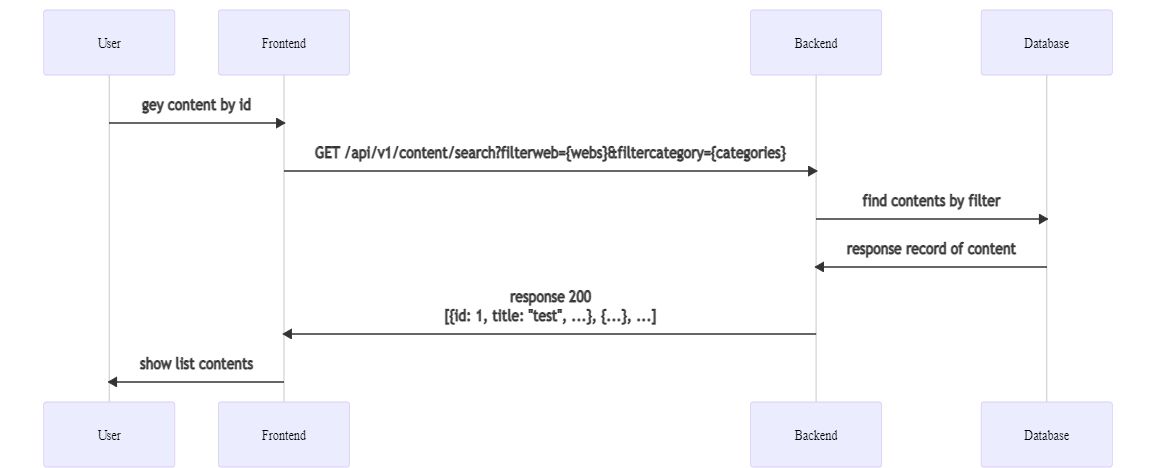
\includegraphics[width=\textwidth]{./img/seq_filter.png}
  \caption{Sequence diagram ของการค้นหาบทความโดยใช้ตัวกรองต่าง ๆ}\label{fig:seq_content_search} 
\end{figure} 
\begin{longtable}[!ht]{p{3cm}|p{8cm}}
  \caption{API Document ของการแสดงรายการค้นหาด้วยตัวกรองต่าง ๆ }\label{tbl:api_content_search} 
    \endfirsthead
    \endhead
    \hhline{==} 
    \textbf{URL}              & \begin{tabular}[c]{@{}l@{}} /api/v1/content/search?filterweb=sanook, \\ true\&filtercategory=sport,politic \end{tabular}                                                                                           \\ \hline
    \textbf{Description}      & แสดงรายการค้นหาด้วยตัวกรองต่าง ๆ                                                                                     \\ \hline
    \textbf{METHOD}           & GET                                                                                                                 \\ \hline
    \textbf{HEADER}           & -                                                                                         \\ \hline
    \textbf{QUERY}            & \begin{tabular}[c]{@{}l@{}}filterweb:\quad\quad string{[}{]} \\ filtercateogry:\quad string{[}{]}\end{tabular}  \\ \hline \hline
    \textbf{Response Status}  & \multicolumn{1}{c}{\textbf{Response Data}}                                                                          \\ \hline
    \multicolumn{1}{c|}{200}  &
    \begin{tabular}[c]{@{}l@{}}{[}\\ \quad\{\\ \quad\quad id: 1,\\ \quad\quad weblink: "www.sanook.com/xxx/yyy",\\\quad\quad status: "success",\\ 
      \quad\quad category: {[}"การเมือง"{]},\\ \quad\quad title: "การประชุมเพื่อการปกครอง"\\ \quad\quad content: "เนื่องด้วย...................."\\ \quad\},\\ 
      \quad\{\\ \quad\quad id: 2,\\ \quad\quad weblink: "www.sanook.com/xxx/yyy",\\\quad\quad status: "success",\\ 
      \quad\quad category: {[}"การเมือง"{]},\\ \quad\quad title: "การประชุมเพื่อการปกครอง"\\ \quad\quad content: "เนื่องด้วย...................."\\ \quad \}\\{]}\end{tabular} \\
    \hhline{==} 
\end{longtable}
\newpage

\subsubsection{ค้นหาบทความโดยใช้เลขอ้างอิงเนื้อหา}
\textbf{Name: }การค้นหาเนื้อหาโดยใช้เลขอ้างอิงเนื้อหา \\
\textbf{Actors: }ผู้ใช้งาน สมาชิก (ผู้ใช้งานที่ลงทะเบียนแล้ว) ผู้จัดการระบบ \\
\textbf{Goal: }ค้นหาบทความตามเลขอ้างอิงเนื้อหา \\
\textbf{Precondition: }- \\
\textbf{Main success scenario: } \\
  \hspace*{0.5cm}1. ผู้ใช้งานทำการค้นหาบทความโดยใช้เลขอ้างอิงเนื้อหา \\
  \hspace*{0.5cm}2. ระบบค้นหาบทความโดยใช้เลขอ้างอิงเนื้อหา \\
  \hspace*{0.5cm}3. ระบบแสดงผลบทความกลับไปยังผู้ใช้งาน  \\
\textbf{Extension (a): } \\
  \hspace*{0.5cm}2a. ระบบไม่พบบทความตามเลขอ้างอิง \\
  \hspace*{0.5cm}3a. ระบบแจ้งผู้ใช้งานว่าไม่พบเนื้อหาตามเลขอ้างอิง \\ 
\begin{figure}[!ht]\centering
  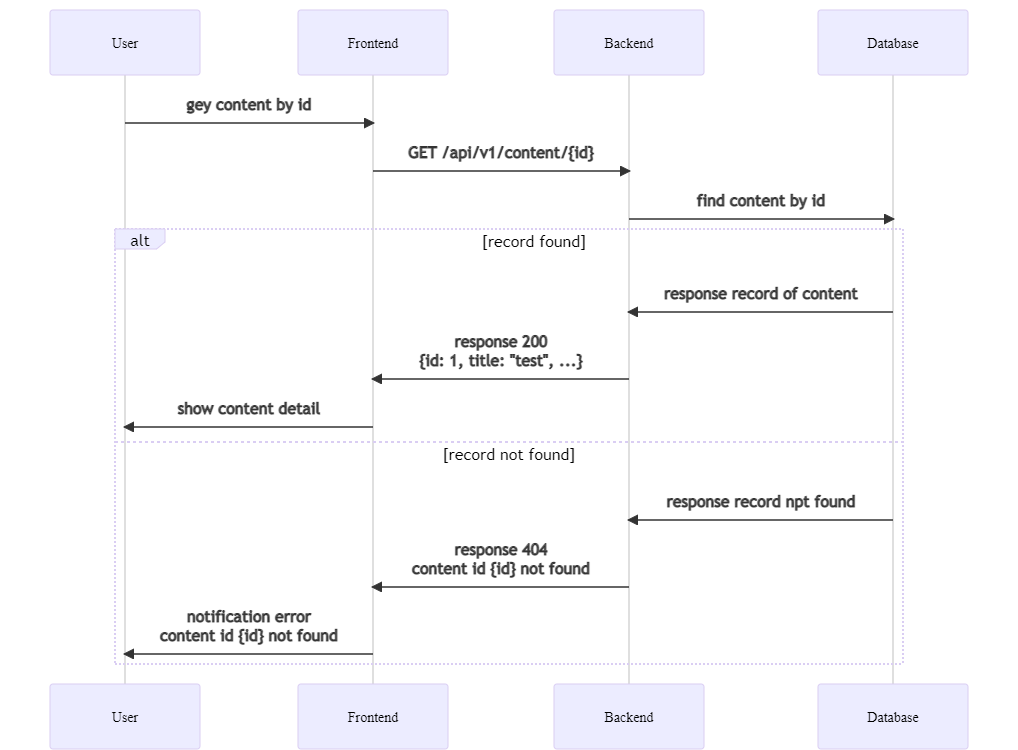
\includegraphics[width=0.95\textwidth]{./img/seq_searchid.png}
  \caption{Sequence diagram ของการค้นหาบทความโดยใช้เลขอ้างอิงเนื้อหา}\label{fig:seq_content_id} 
\end{figure} 
\begin{longtable}[!ht]{p{3cm}|p{8cm}}
  \caption{API Document ของการแสดงผลข้อมูลเกี่ยวกับเนื้อหาตามเลขอ้างอิงเนื้อหา  }\label{tbl:api_content_id} 
    \endfirsthead
    \endhead
    \hhline{==} 
    \textbf{URL}              & /api/v1/content/{id}                                                                                             \\ \hline
    \textbf{Description}      & แสดงผลข้อมูลเกี่ยวกับเนื้อหาตามเลขอ้างอิงเนื้อหา                                                                                     \\ \hline
    \textbf{METHOD}           & GET                                                                                                                 \\ \hline
    \textbf{HEADER}           & -                                                                                         \\ \hline
    \textbf{PAYLOAD}          & \begin{tabular}[c]{@{}l@{}}url: string\end{tabular}  \\ \hline \newpage \hline
    \textbf{Response Status}  & \multicolumn{1}{c}{\textbf{Response Data}}                                                                          \\ \hline
    \multicolumn{1}{c|}{200}  &
    \begin{tabular}[c]{@{}l@{}}\{\\ \quad id: 1,\\ \quad weblink: ""www.sanook.com/xxx/yyy"",\\ \quad status: "success",\\ 
      \quad category: {[}"การเมือง"{]},\\ \quad title: "การประชุมเพื่อการปกครอง"\\ \quad content: "เนื่องด้วย...................."\\ \}\end{tabular}  \\ \hline
    \multicolumn{1}{c|}{404}  &
    \begin{tabular}[c]{@{}l@{}}\{\\ \quad errors: {[}\\ \quad\quad\{\\ \quad\quad\quad"message": "content id 1 doesn't not exist"\\ \quad\quad\}\\\quad {]}\\ \}\end{tabular}                                                                         \\ \hline
    \hhline{==} 
\end{longtable}

\section{โครงสร้างฐานข้อมูล}
\begin{figure}[!ht]\centering
  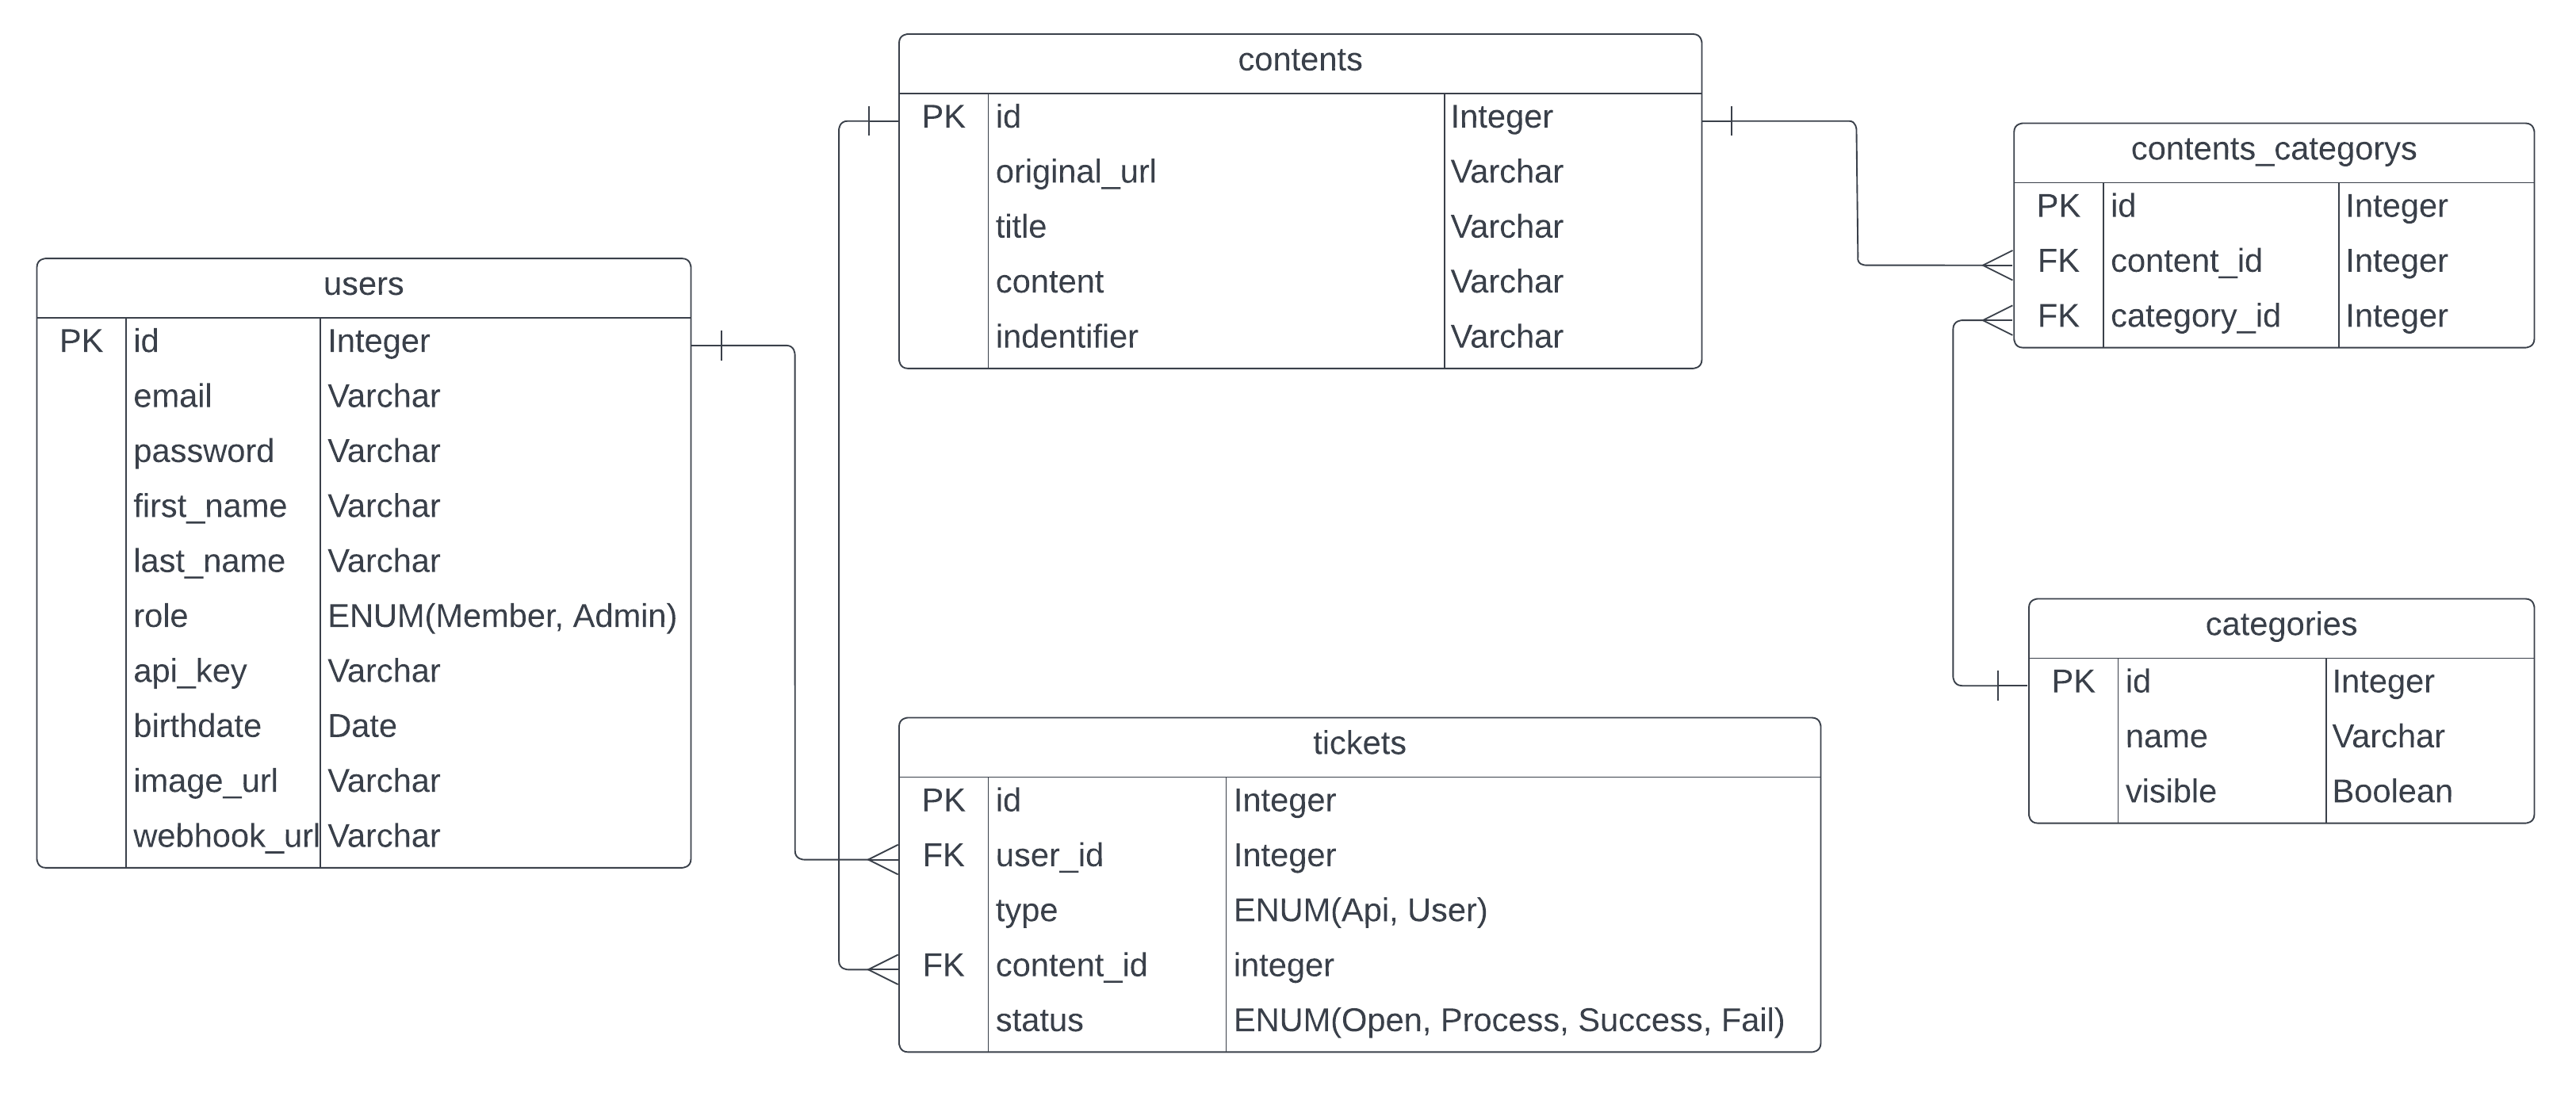
\includegraphics[width=\textwidth]{./img/database.png}
  \caption{โครงสร้างฐานข้อมูล}\label{fig:database} 
\end{figure}

\begin{longtable}{p{0.03\textwidth}|p{0.1\textwidth}|p{0.1\textwidth}|m{0.14\textwidth}|p{0.26\textwidth}|p{0.2\textwidth}}
  \caption{ตารางข้อมูลของสมาชิกในระบบ}\label{tbl:users}  \\
  \hhline{======} 
  \textbf{Key} & \textbf{Attribute} & \textbf{Domain} & \multicolumn{1}{c|}{\textbf{Null}} & \textbf{Description} & \textbf{Example}   \\ \hline
  \endhead
  %
  \textbf{PK}  & id  & int  & \multicolumn{1}{c|}{No}  & เลขสำหรับระบุตัวตนผู้ใช้งานเป็นตัวเลขต่อเนื่องไม่ซ้ำ & 1                  \\ \hline
  \textbf{} & password & varchar(64) & \multicolumn{1}{c|}{No} & รหัสผ่านของบัญชีผู้ใช้ที่ต้องการเข้าสู่ระบบที่ถูกเข้ารหัสด้วย Argon2 algorithm & \$argon2d\$v=19\$m=12, t=3,p=1\$MGtvM3Rzc2R 6bWpjMDAwMA\$09LkH+ 4Z7FPBQsVfa3O2rw \\ \hline
  \textbf{}   & first\_name        & varchar(64)     & \multicolumn{1}{c|}{No}                  & ชื่อของผู้ใช้งาน                                      & พลวัต              \\ \hline
  \textbf{}   & last\_name         & varchar(64)     & \multicolumn{1}{c|}{No}                  & นามสกุลของผู้ใช้งาน                                   & สุภารัตน์          \\ \hline
  \textbf{}   & email              & varchar(64)     & \multicolumn{1}{c|}{No}                  & อีเมลล์ของผู้ใช้งาน ซึ่งจะไม่ซ้ำกับผู้ใช้งานคนอื่น ๆ  & ponlawat@gmail.com \\ \hline
  \textbf{}   & role               & varchar(64)     & \begin{tabular}[c]{@{}c@{}} ENUM \\ (Member, Admin) \end{tabular} & สิทธิ์การเข้าใช้งาน                                   & Admin              \\ \hline
  \textbf{}   & api\_key & varchar(255) & \multicolumn{1}{c|}{Yes} &  รหัสสำหรับการยืนยันตัวตนการเข้าใช้งานผ่านระบบภายนอก & 8d969eef6ecad3c29a3a 629280e686cf0c3f5d5a86 aff3ca12020c923adc6c92 \\ \hline
  \textbf{}   & birthdate        & date     & \multicolumn{1}{c|}{No}                  & วันเกิดในรูปแบบ พ.ศ.                                      & 22/01/2544              \\ \hline
  \textbf{}   & image\_url        & varchar(64)     & \multicolumn{1}{c|}{Yes}          & ลิงก์สำหรับเก็บรูปภาพ                                     & www.abc.com/profile.png              \\ \hline
  \textbf{}   & webhook\_url        & varchar(64)     & \multicolumn{1}{c|}{Yes}          & ลิงก์ Url สำหรับส่งข้อมูลกลับ                           & www.efg.com/content/webhook            \\
  \hhline{======}  
\end{longtable}

\begin{longtable}{p{0.03\linewidth}|p{0.1\linewidth}|p{0.17\linewidth}|m{0.03\linewidth}|p{0.4\linewidth}|p{0.1\linewidth}}
  \caption{ตารางข้อมูลคำร้องขอการวิเคราะห์หมวดหมู่ของบทความ}\label{tbl:ticket}  \\
  \hhline{======} 
  \textbf{Key} & \textbf{Attribute} & \textbf{Domain} & \textbf{Null} & \textbf{Description} &\multicolumn{1}{c}{\textbf{Example}}  \\ \hline
  \endfirsthead
  %
  \endhead
  %
  \textbf{PK} & id      & int         & No & เลขสำหรับระบุอ้างอิงเนื้อหาเป็นตัวเลขต่อเนื่องไม่ซ้ำ      & \multicolumn{1}{c}{1}          \\ \hline
  \textbf{FK} & user\_id & int         & No & เลขสำหรับระบุตัวตนผู้ใช้งาน                       & \multicolumn{1}{c}{2}     \\ \hline
  \textbf{ }   & type & Enum(Api, User)     & No & ประเภทของการสร้างคำร้องขอ                 & \multicolumn{1}{c}{User}        \\ \hline
  \textbf{FK} & content\_id & int         & No & เลขสำหรับระบุอ้างอิงเนื้อหา                       & \multicolumn{1}{c}{3}     \\ \hline
  \textbf{ }   & status & Enum(Open, Processing, Success, Fail)         & No & สถานะการดำเนินของการร้องขอ   & \multicolumn{1}{c}{Processing}     \\ 
  \hhline{======}
\end{longtable}

\begin{longtable}{p{0.03\linewidth}|p{0.1\linewidth}|p{0.1\linewidth}|m{0.03\linewidth}|p{0.27\linewidth}|p{0.3\linewidth}}
  \caption{ตารางบทความที่ทำการวิเคราะห์} \label{tbl:content}\\
  \hhline{======}
  \textbf{Key} & \textbf{Attribute} & \textbf{Domain} & \textbf{Null} & \textbf{Description} & \textbf{Example} \\ \hline
  \endfirsthead
  %
  \endhead
  %
  \textbf{PK} & id & int &  No & เลขสำหรับระบุอ้างอิงเนื้อหาเป็นตัวเลขต่อเนื่องไม่ซ้ำ & 1 \\\hline
  \textbf{} & original\_url & varchar(255) & Yes & ลิ้งค์ url ที่ต้องการวิเคราะห์เนื้อหา & https://www.sanook.com/money/888331/ \\\hline
  \textbf{} & title & varchar(255) & Yes & หัวข้อของเนื้อหาที่ต้องการวิเคราะห์ & APEC 2022 พาณิชย์ ยกขบวนสินค้า GI ขึ้นเวทีเอเปค \\ \hline
  \textbf{} & content & text & Yes & เนื้อหาที่ต้องการวิเคราะห์ & พาณิชย์ ยกขบวนสินค้า GI ร่วมต้อนรับสุดยอดผู้นำในการประชุมเอเปค 2022 Soft Power นำอัตลักษณ์ท้องถิ่นไทยสู่สายตาชาวโลก นายวุฒิไกร ลีวีระพันธุ์ อธิบดีกร....... \\ \hline
  \textbf{} & indentifier & varchar(64) & Yes & ตัวอ้างอิงเนื้อหาซึ่งจะอยู่ในรูปแบบ \{website\}:\{reference\} & sanook:money/888331 \\ 
  \hhline{======}
\end{longtable}

\begin{longtable}{p{0.03\linewidth}|p{0.1\linewidth}|p{0.1\linewidth}|m{0.03\linewidth}|p{0.47\linewidth}|p{0.1\linewidth}}
  \caption{ตารางหมวดหมู่ที่ใช้งานภายในระบบ}\label{tbl:categories}  \\
  \hhline{======}
  \textbf{Key} & \textbf{Attribute} & \textbf{Domain} & \textbf{Null} & \textbf{Description} &\multicolumn{1}{c}{\textbf{Example}}  \\ \hline
  \endfirsthead
  %
  \endhead
  %
  \textbf{PK} & id      & int         & No & เลขสำหรับระบุอ้างอิงเนื้อหาเป็นตัวเลขต่อเนื่องไม่ซ้ำ      & \multicolumn{1}{c}{1}          \\ \hline
  \textbf{}   & name    & varchar(64) & No & ชื่อของประเภทหมวดหมู่                          & \multicolumn{1}{c}{การเมือง}     \\ \hline
  \textbf{}   & visible & boolean     & No & สถานะการแสดงผลให้ผู้อื่นเห็น                     & \multicolumn{1}{c}{TRUE}        \\ \hhline{======}
\end{longtable}

\begin{longtable}{p{0.03\linewidth}|p{0.12\linewidth}|p{0.08\linewidth}|m{0.03\linewidth}|p{0.47\linewidth}|p{0.1\linewidth}}
  \caption{ตารางความสัมพันธ์ของเนื้อหากับหมวดหมู่ต่าง ๆ}\label{tbl:content_categories}  \\
  \hhline{======}
  \textbf{Key} & \textbf{Attribute} & \textbf{Domain} & \textbf{Null} & \textbf{Description} &\multicolumn{1}{c}{\textbf{Example}}  \\ \hline
  \endfirsthead
  %
  \endhead
  %
  \textbf{PK} & id      & int         & No & เลขสำหรับระบุอ้างอิงเนื้อหาเป็นตัวเลขต่อเนื่องไม่ซ้ำ      & \multicolumn{1}{c}{1}          \\ \hline
  \textbf{FK}   & content\_id    & int & No & เลขสำหรับระบุอ้างอิงเนื้อหา                          & \multicolumn{1}{c}{3}     \\ \hline
  \textbf{FK}   & category\_id & int     & No & เลขสำหรับระบุอ้างอิงหมวดหมู่                     & \multicolumn{1}{c}{4}        \\ \hhline{======}
\end{longtable}

\section{User Interface Design}
\subsection{User Interface Design Rule}
การออกแบบเว็บแอปพลิเคชัน AI Platform Thai Content Tagging มีหลักการออกแบบดังนี้
\begin{itemize}
  \item มีการป้องกันการผิดพลาดของการกรอกข้อมูลใน Form เพื่อไม่ให้มีปัญหาต่อผู้ใช้และระบบ
  \item มี Navbar เพื่อสามารถให้ผู้ใช้ไปยังหน้าที่ต้องการได้
  \item มี Response กลับมายังผู้ใช้งานในการกระทำนั้น ๆ ทุกครั้ง
  \item ไม่เปลี่ยนแปลงพฤติกรรมที่ผู้ใช้งานคุ้นเคย เช่น ตำแหน่งของปุ่มต่าง ๆ
  \item ใช้ Font OldNewpaperTypes, Poppins และ Lato
  \item โทนสีในการออกแบบ 
        \begin{figure}[!ht]\centering
          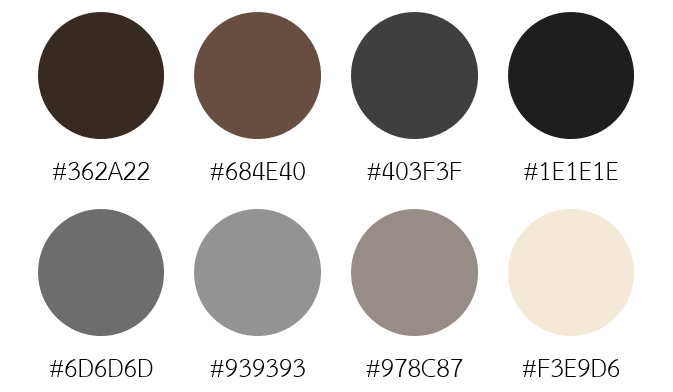
\includegraphics[height=3.5cm]{./img/color.png} 
        \end{figure}
\end{itemize}

\newpage
\subsection{User Interface สำหรับผู้ใช้งาน}
\subsubsection{หน้า Landing}
  \begin{figure}[!ht]\centering
    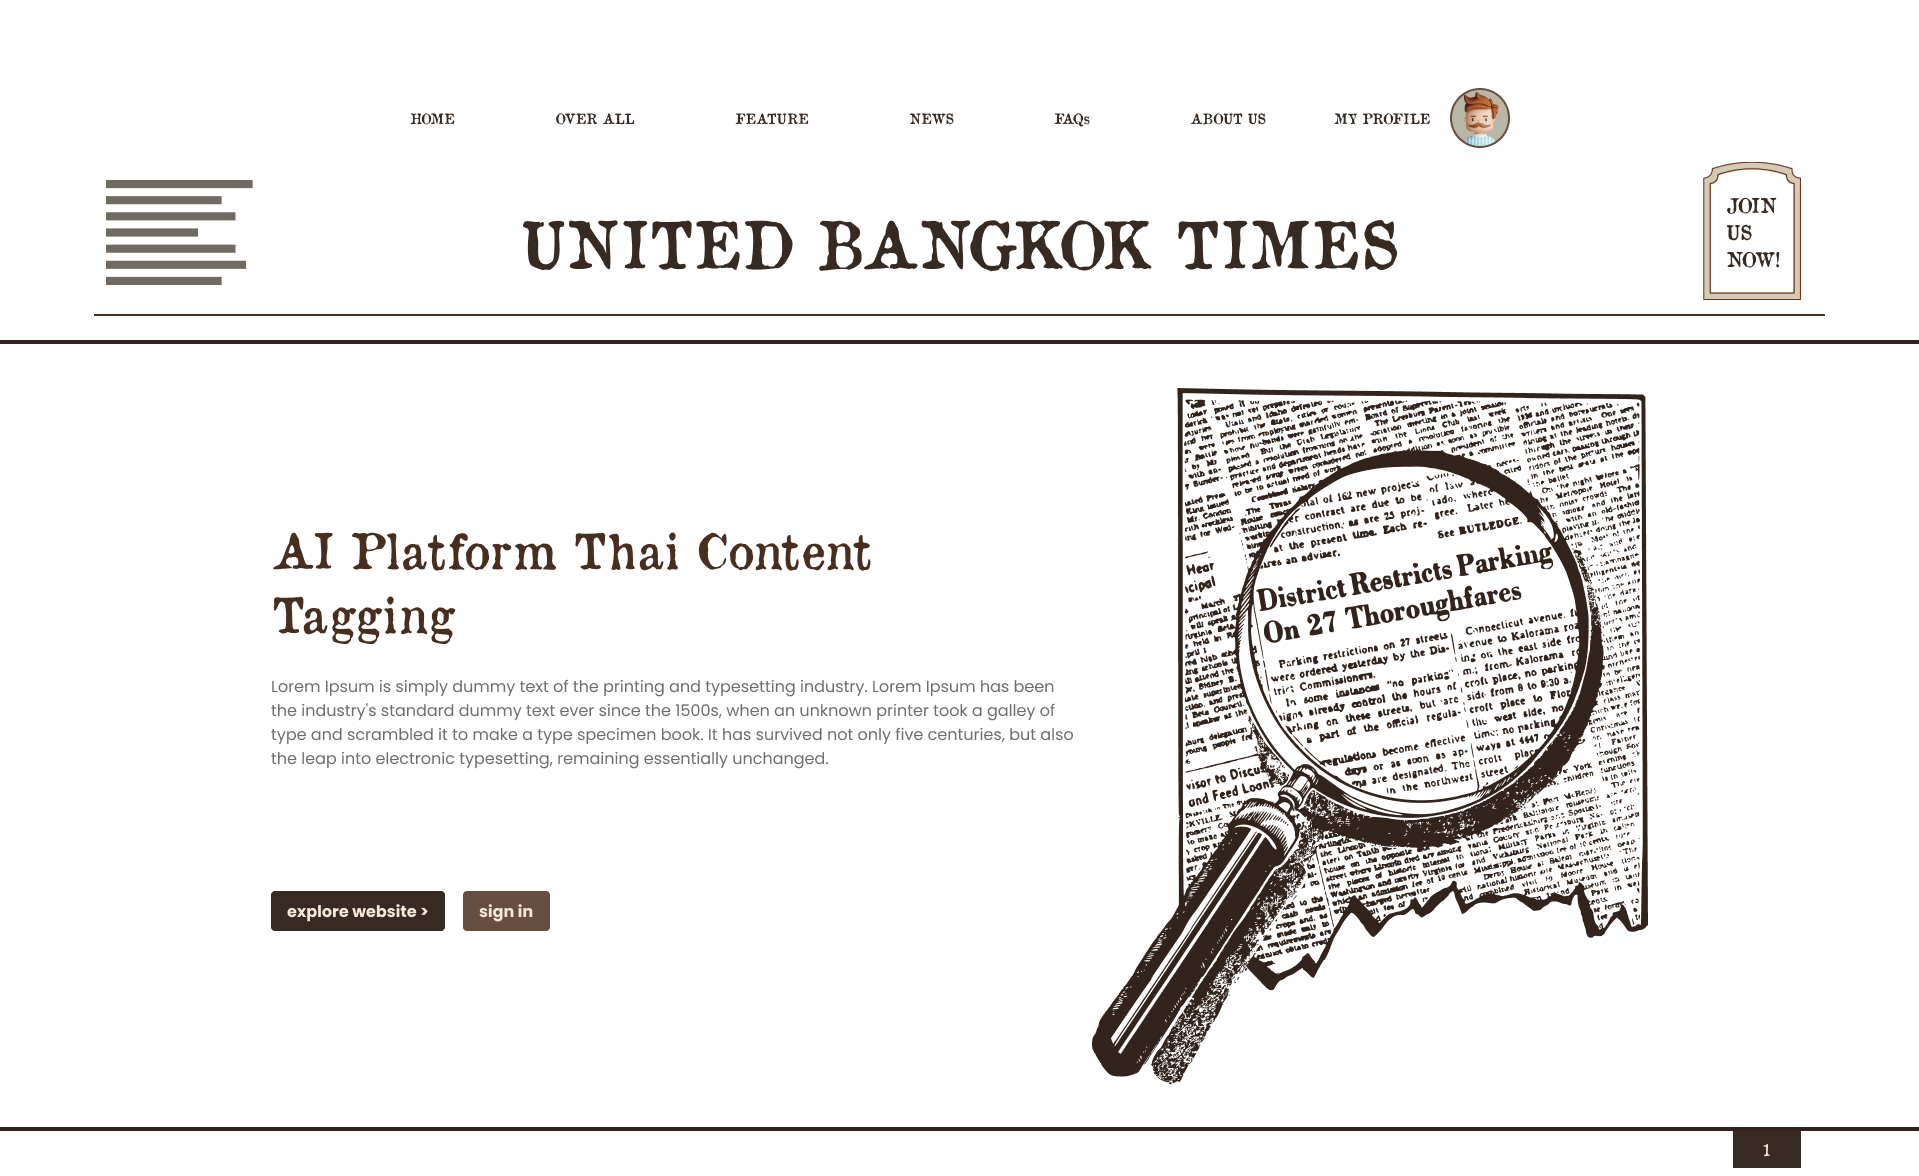
\includegraphics[width=15cm]{./img/project_ui/landing_page1.png} 
    \caption{หน้า Landing}\label{fig:landing_page_1} 
  \end{figure}
  \hspace*{1cm}เป็นหน้าแรกของเว็บแอปพลิเคชันที่ผู้ใช้งานจะได้พบเจอ 
  ซึ่งหน้า Landing เป็นหน้าที่ผู้ใช้งานทั่วไปและสมาชิกสามารถเข้าถึงได้ โดยที่ผู้ใช้งานทั่วไปสามารถเลือกได้ว่าจะรับชมเว็บแอปพลิเคชันหรือจะสมัครสมาชิก 
  โดยหน้า Landing page จะเป็นหน้าที่แสดงให้ผู้ใช้งานทั่วไปและสมาชิกทราบได้ว่าเว็บไซต์นี้เป็นเว็บแอปพลิเคชันเกี่ยวกับอะไรและสามารถใช้งานอย่างไร

  \begin{figure}[!ht]\centering
    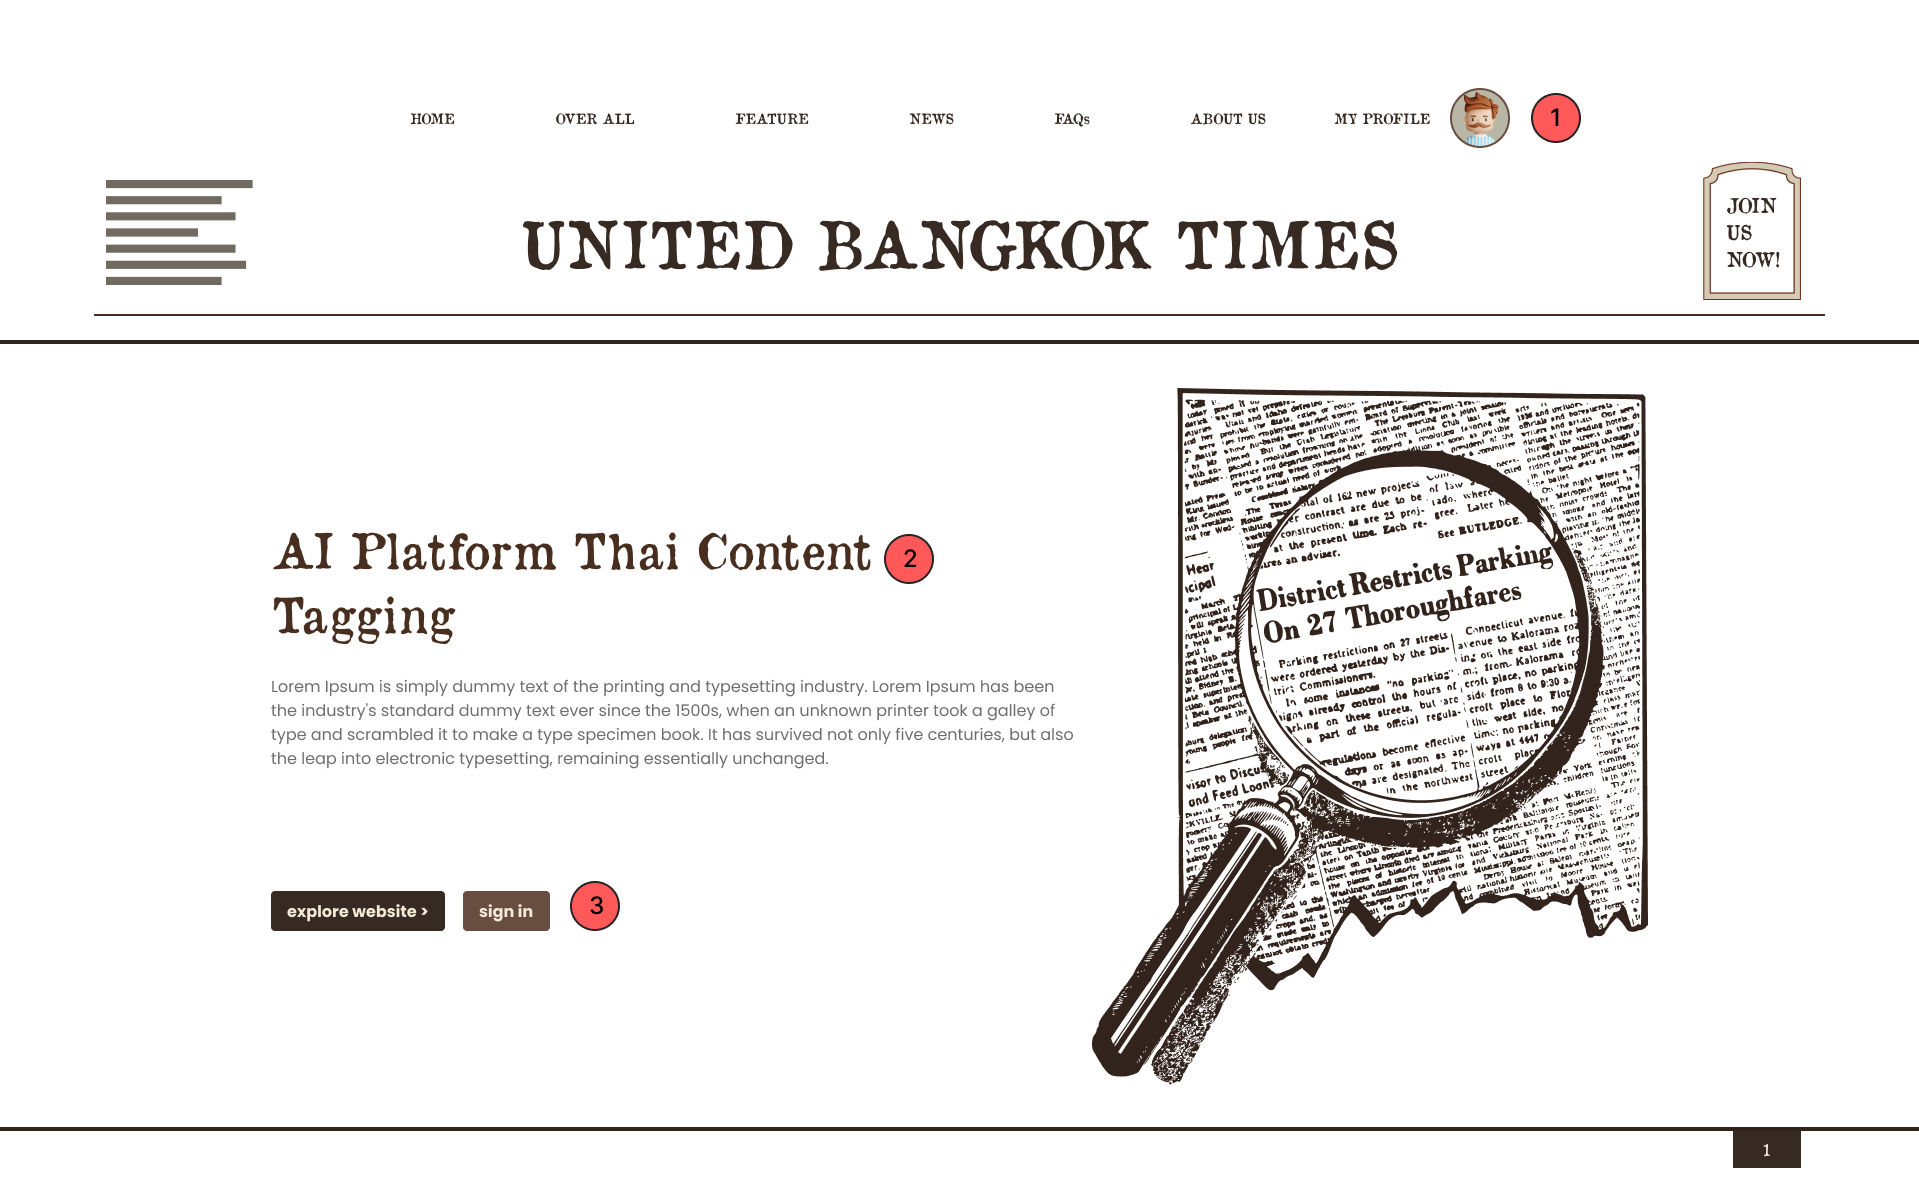
\includegraphics[width=15cm]{./img/project_ui/landing_page2.png} 
    \caption{Landing page ที่แสดงแต่ละองค์ประกอบ}\label{fig:landing_page_2} 
  \end{figure}
  \hspace*{1cm}ในภาพนี้ (รูปที่:\ref{fig:landing_page_2}) จะมีอยู่ 3 ส่วนด้วยกัน ได้แก่
  \begin{enumerate}
    \item Navigation Bar (NavBar) เป็นส่วนที่จะนำพาผู้ใช้งานไปยังหน้าอื่น ๆ 
          ซึ่งผู้ใช้งานสามารถเลือกดูหน้าเว็บแอปพลิเคชันทั้งหมดคร่าว ๆ ได้ โดยแต่ละหน้าก็จะบอกรายละเอียดเกี่ยวกับเว็บแอปพลิเคชัน
    \item ส่วนรายละเอียดเว็บแอปพลิเคชัน เป็นส่วนที่จะอธิบายรายละเอียดและการทำงานของเว็บแอปพลิเคชันคร่าว ๆ เพื่อให้ผู้ใช้งานรู้จักและเข้าใจแนวคิดของเว็บแอปพลิเคชันมากขึ้น
    \item หากผู้ใช้งานต้องการเข้าชมหรือศึกษารายละเอียดของเว็บแอปพลิเคชันมากขึ้น ผู้ใช้งานสามารถเลือกคลิกที่ Explore Website ได้ ซึ่งเว็บแอปพลิเคชันก็จะพาผู้ใช้งานไปยังหน้า Home Page (รูปที่:\ref{fig:homepage})
          หรือถ้าหากผู้ใช้งานต้องการเข้าสู่ระบบ ผู้ใช้งานสามารถเลือกคลิกที่ Sign In ได้ ซึ่งเว็บแอปพลิเคชันก็จะแสดงหน้า Sign In เพื่อให้ผู้ใช้งานได้ทำการเข้าสู่ระบบ (รูปที่:\ref{fig:login})
  \end{enumerate}
  \begin{figure}[!ht]\centering
    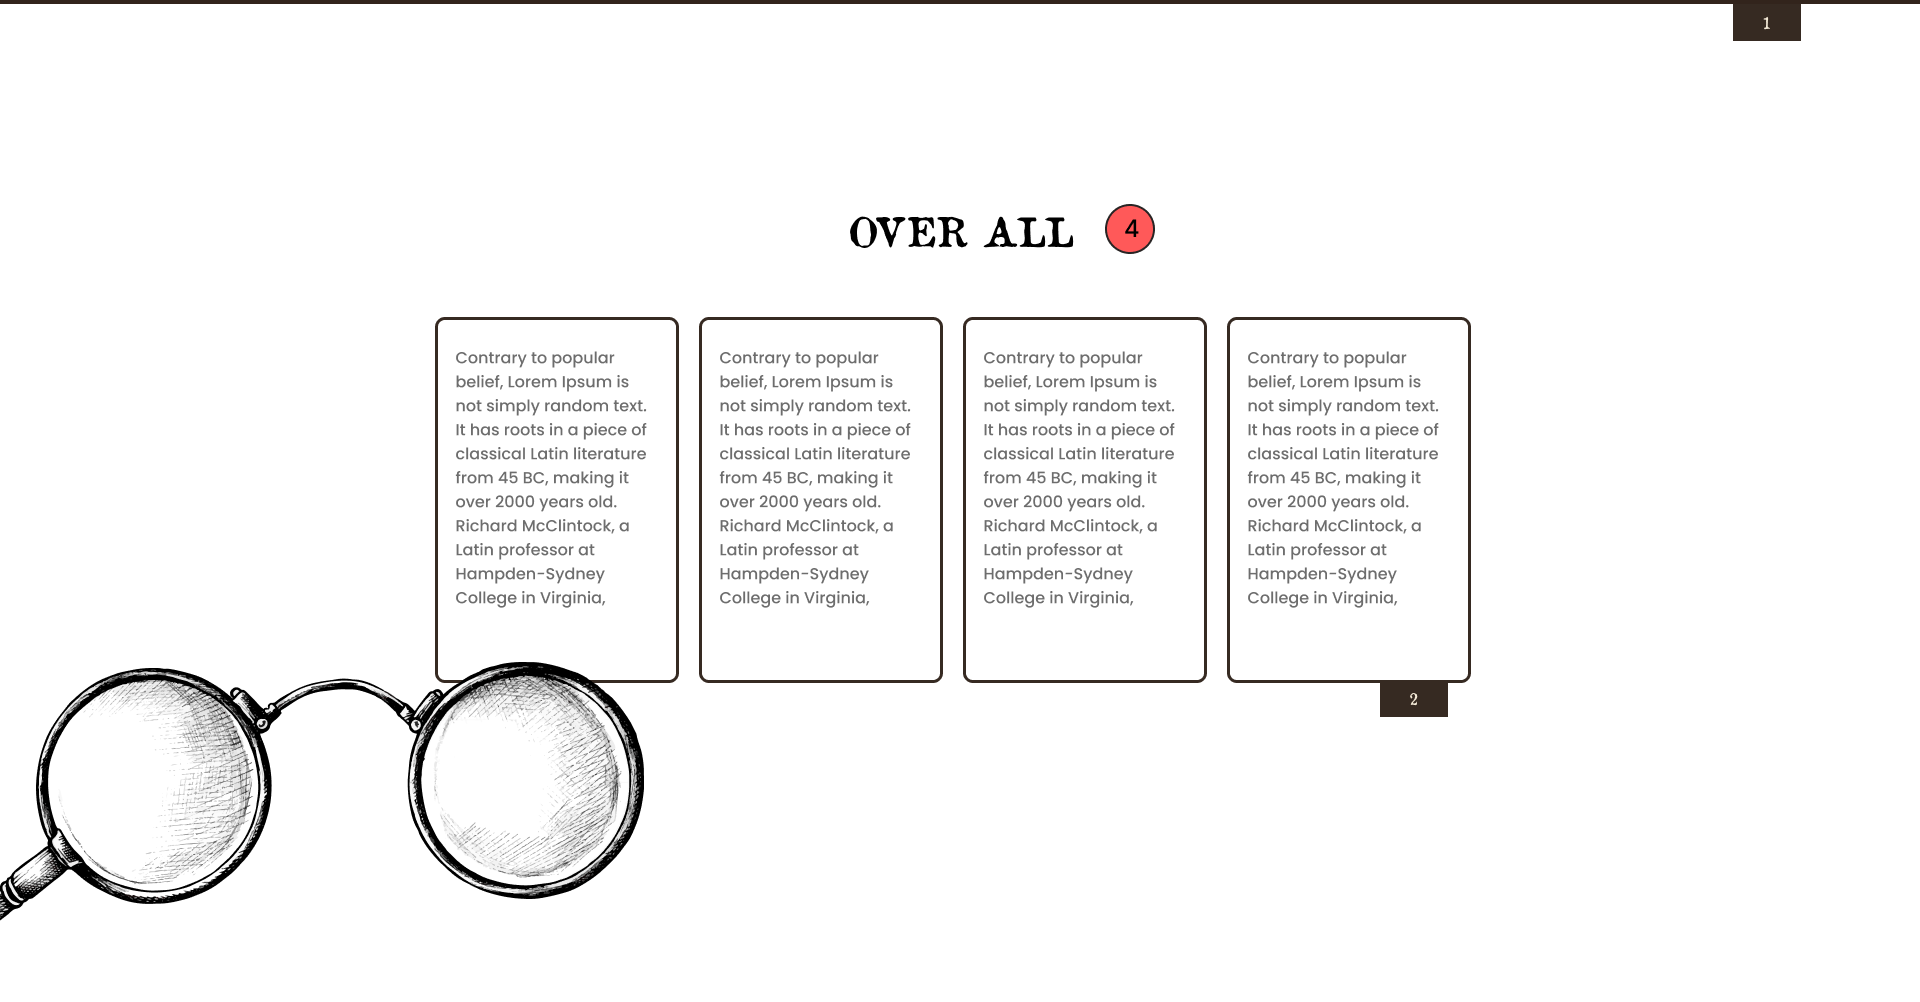
\includegraphics[width=14cm]{./img/project_ui/overall.png} 
    \caption{หน้า Landing ในส่วนของ Overall}\label{fig:overall} 
  \end{figure}
  \hspace*{1cm}ในส่วนที่ 4 จะเป็นส่วนที่ยังคงอยู่ในหน้า Landing Page โดยเป็นส่วนที่ให้ข้อมูลและรายละเอียดเกี่ยวกับเว็บแอปพลิเคชัน AI Platform Thai Content Tagging
  ว่าเว็บแอปพลิเคชันนี้ให้ Service ที่มีบริการใดบ้าง
  \begin{figure}[!ht]\centering
    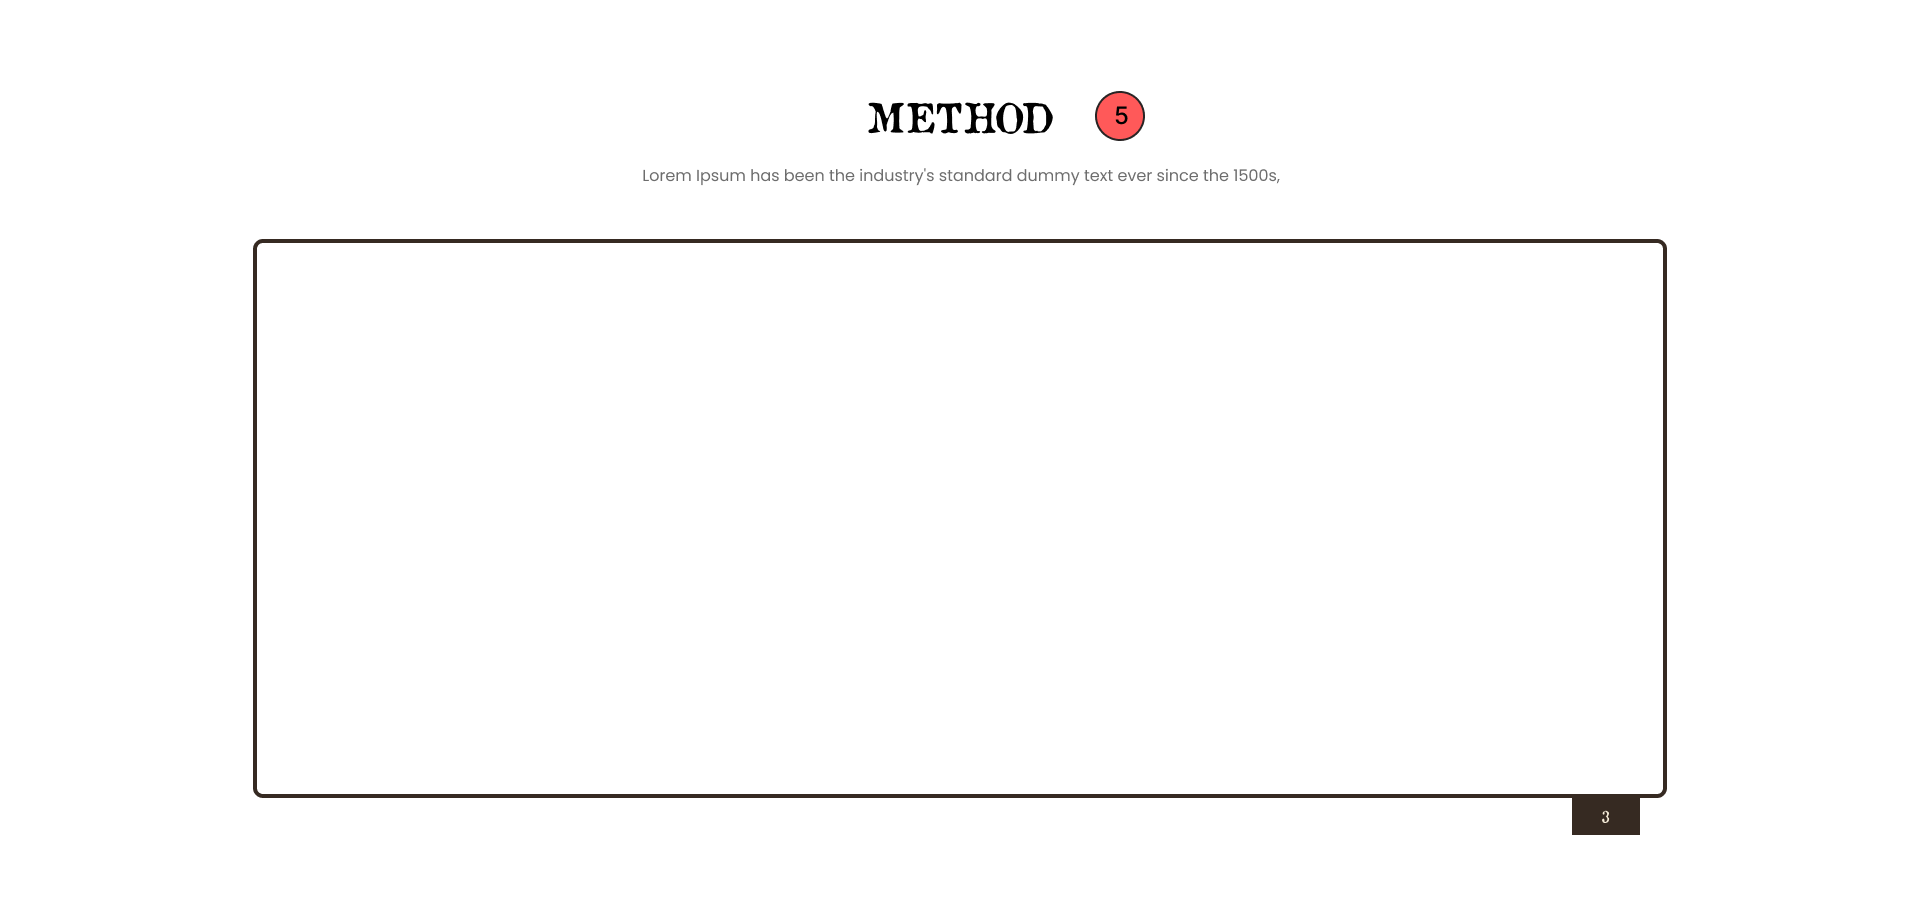
\includegraphics[width=14cm]{./img/project_ui/method.png} 
    \caption{หน้า Landing ในส่วนของ Method}\label{fig:method} 
  \end{figure}
  \newline\hspace*{1cm}ในส่วนที่ 5 จะเป็นส่วนที่ยังคงอยู่ในหน้า Landing Page โดยเป็นส่วนที่แสดงกระบวนการการทำงานของเว็บแอปพลิเคชัน AI Platform Thai Content Tagging

  \begin{figure}[!ht]\centering
    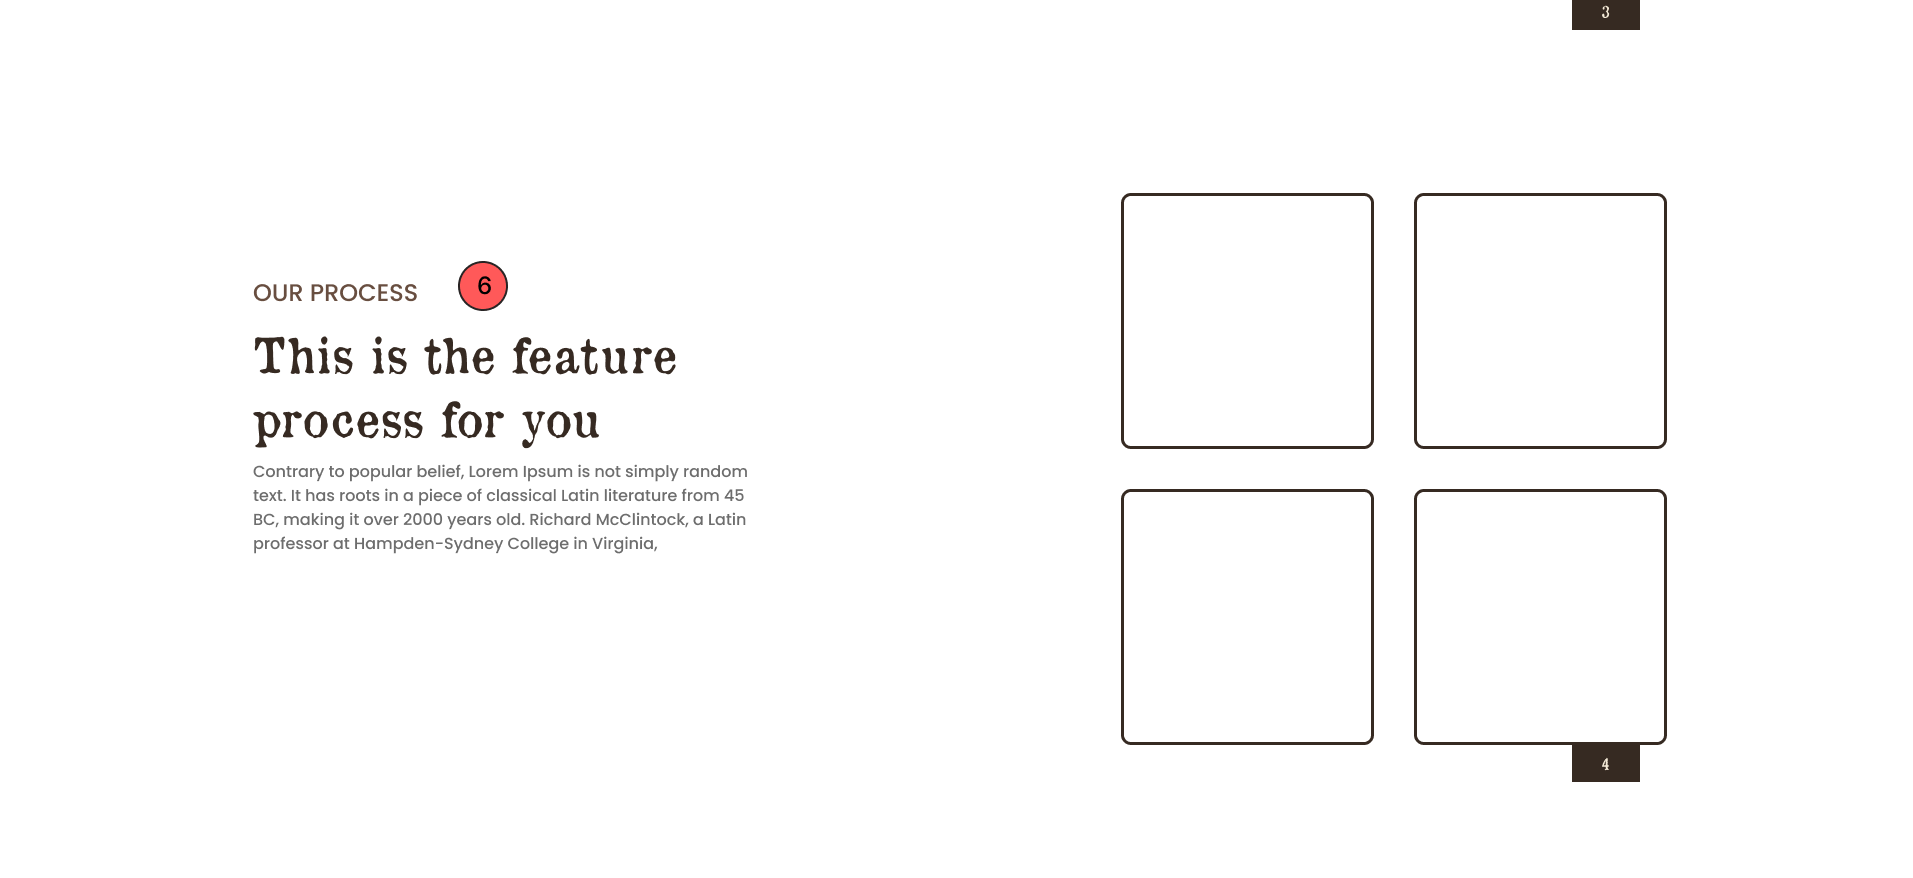
\includegraphics[width=13cm]{./img/project_ui/feature.png} 
    \caption{หน้า Landing ในส่วนของ Feature}\label{fig:feature_ui} 
  \end{figure}
  \hspace*{1cm}ในส่วนที่ 6 จะเป็นส่วนที่ยังคงอยู่ในหน้า Landing Page โดยเป็นส่วนที่อธิบายให้ผู้ใช้งานทราบว่าผู้ใช้งานจะสามารถใช้งานบริการของเว็บแอปพลิเคชัน AI Platform Thai Content Tagging
  ได้อย่างไร

\subsubsection{หน้า Login}
\begin{figure}[!ht]\centering
  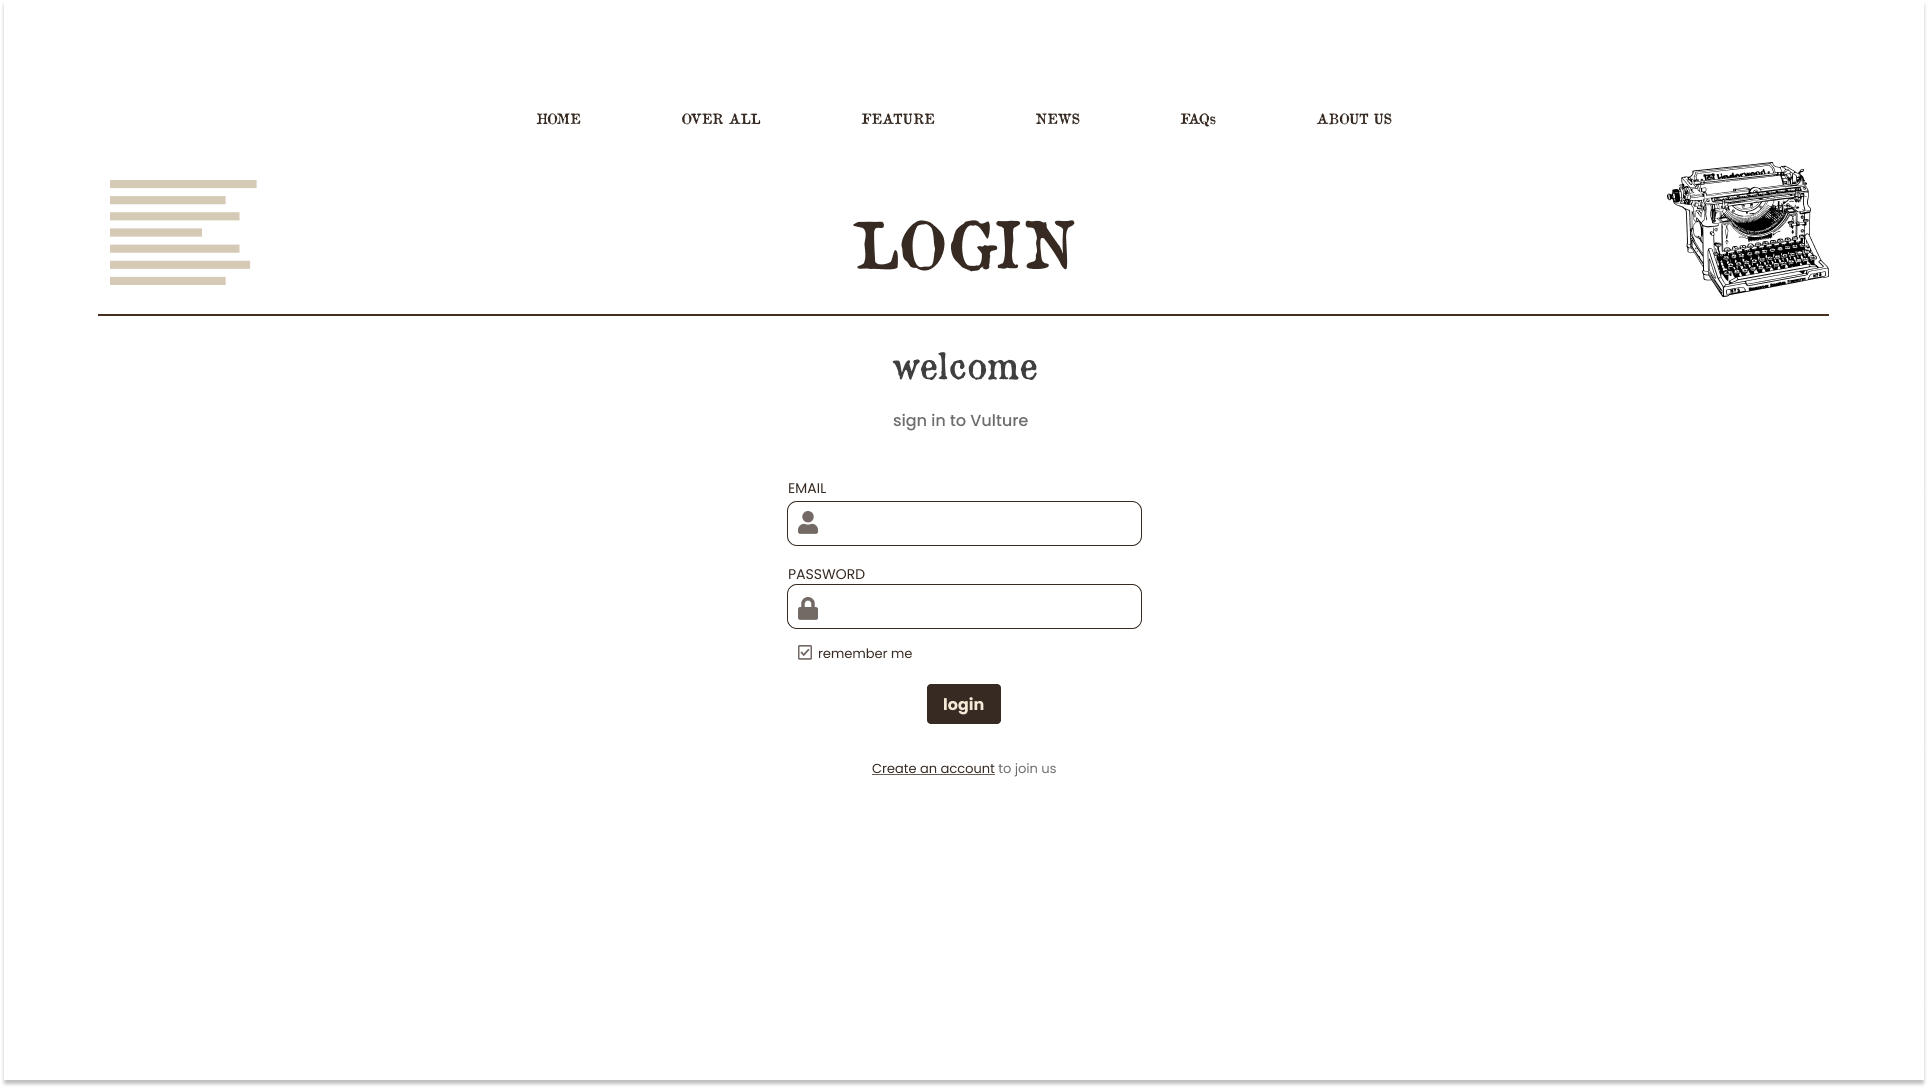
\includegraphics[width=14cm]{./img/project_ui/login.png} 
  \caption{หน้า Login}\label{fig:login} 
\end{figure}
\hspace*{1cm}เป็นหน้าสำหรับผู้ใช้งานที่ต้องการเข้าสู่ระบบเพื่อใช้บริการของเว็บแอปพลิเคชัน AI Platform Thai Content Tagging 
โดยหากผู้ใช้งานทำการกรอก Email และ Password ที่ถูกต้อง เว็บแอปพลิเคชันก็จะพาผู้ใช้งานไปยังหน้า Home Page (รูปที่:\ref{fig:homepage})
ซึ่งในหน้า Login จะมีองค์ประกอบต่าง ๆ ได้แก่ 
\begin{itemize}
  \item Email เป็นส่วนสำหรับกรอก Email ที่ใช้ในการเข้าสู่ระบบ
  \item Password เป็นส่วนสำหรับกรอก Password ที่ใช้ในการเข้าสู่ระบบ
  \item Remember Me เป็นส่วนที่จดจำ Username และ Password เพื่อให้สามารถเข้าสู่ระบบได้ทันทีในครั้งถัดไป
  \item Create an account หากกรณีที่ผู้ใช้งานยังไม่มีบัญชี ผู้ใช้งานสามารถสมัครบัญชีได้ด้วยการคลิกที่ Create an account เว็บแอปพลิเคชันก็จะพาผู้ใช้งานไปยังหน้า Register (รูปที่:\ref{fig:register})
\end{itemize}
\begin{figure}[!ht]\centering
  
\includegraphics[width=8cm]{./img/project_ui/login_fail.png} 
  \caption{กรอก Username หรือ Password ผิดพลาด}\label{fig:login_fail} 
\end{figure}
\hspace*{1cm}กรณีที่ผู้ใช้งานกรอก Email และ Password ผิดพลาด เว็บแอปพลิเคชันจะทำการแจ้งเตือนให้ผู้ใช้งานทราบและให้ผู้ใช้งานกรอก Email และ Password ใหม่อีกครั้ง

\subsubsection{หน้า Register}
\begin{figure}[!ht]\centering
  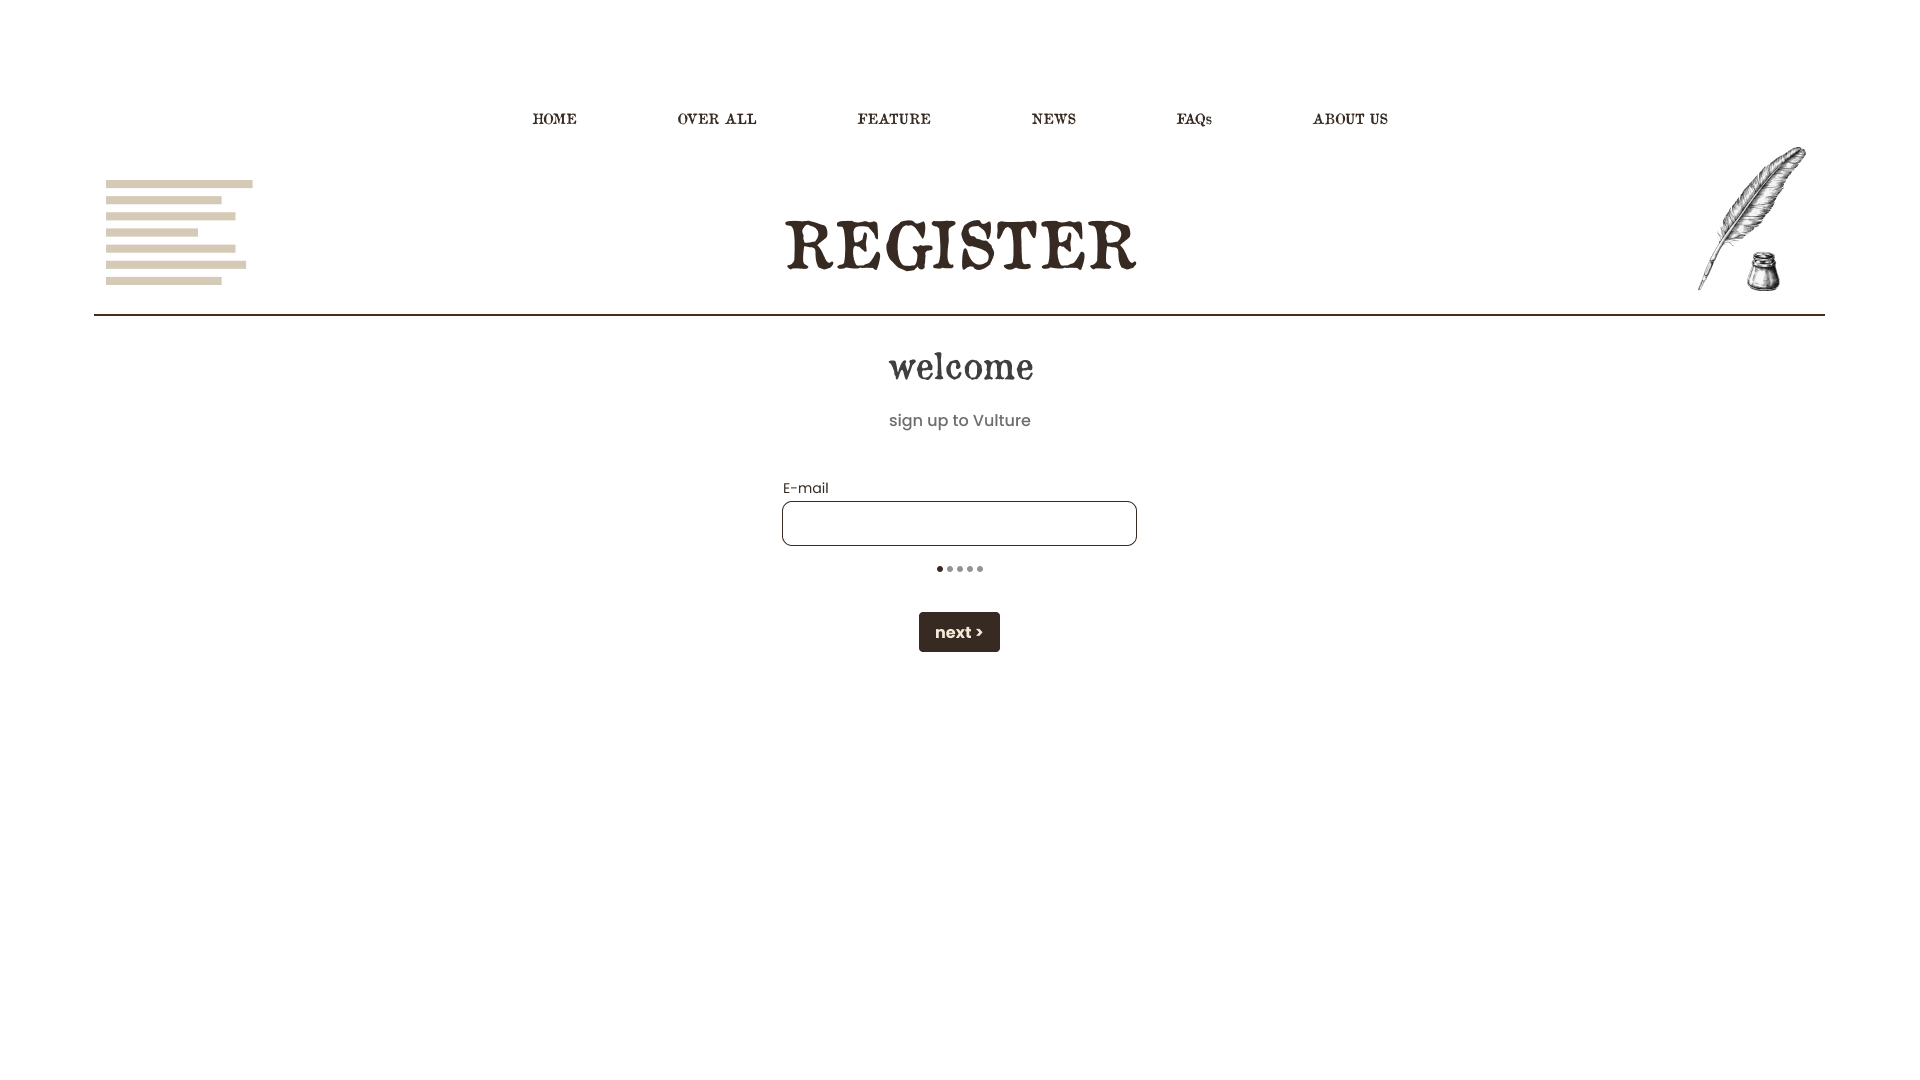
\includegraphics[width=16cm]{./img/project_ui/4.png} 
  \caption{หน้า Register ขั้นตอนกรอก Email}\label{fig:register} 
\end{figure}
\hspace*{1cm}เป็นหน้าสำหรับผู้ใช้งานที่ต้องการสมัครสมาชิกเพื่อเป็นสมาชิกของเว็บแอปพลิเคชัน AI Platform Thai Content Tagging 
โดยหากผู้ใช้งานทำการกรอก Email ถูกต้อง เว็บแอปพลิเคชันก็จะพาผู้ใช้งานไปยังหน้า Register ในขั้นตอนถัดไป (รูปที่:\ref{fig:register_password})
\begin{figure}[!ht]\centering
  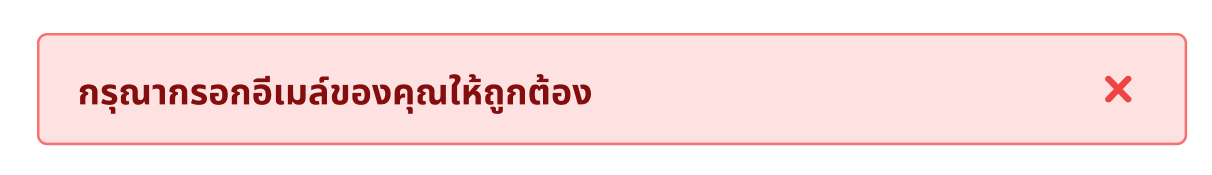
\includegraphics[width=9cm]{./img/project_ui/wrong_email.png} 
  \caption{กรอก Email ผิดพลาด}\label{fig:wrong_email} 
\end{figure}
\newline\hspace*{1cm}กรณีที่ผู้ใช้งานกรอก Email ผิดพลาด เว็บแอปพลิเคชันจะทำการแจ้งเตือนให้ผู้ใช้งานทราบและให้ผู้ใช้งานกรอก Email ใหม่อีกครั้ง \newpage
\begin{figure}[!ht]\centering
  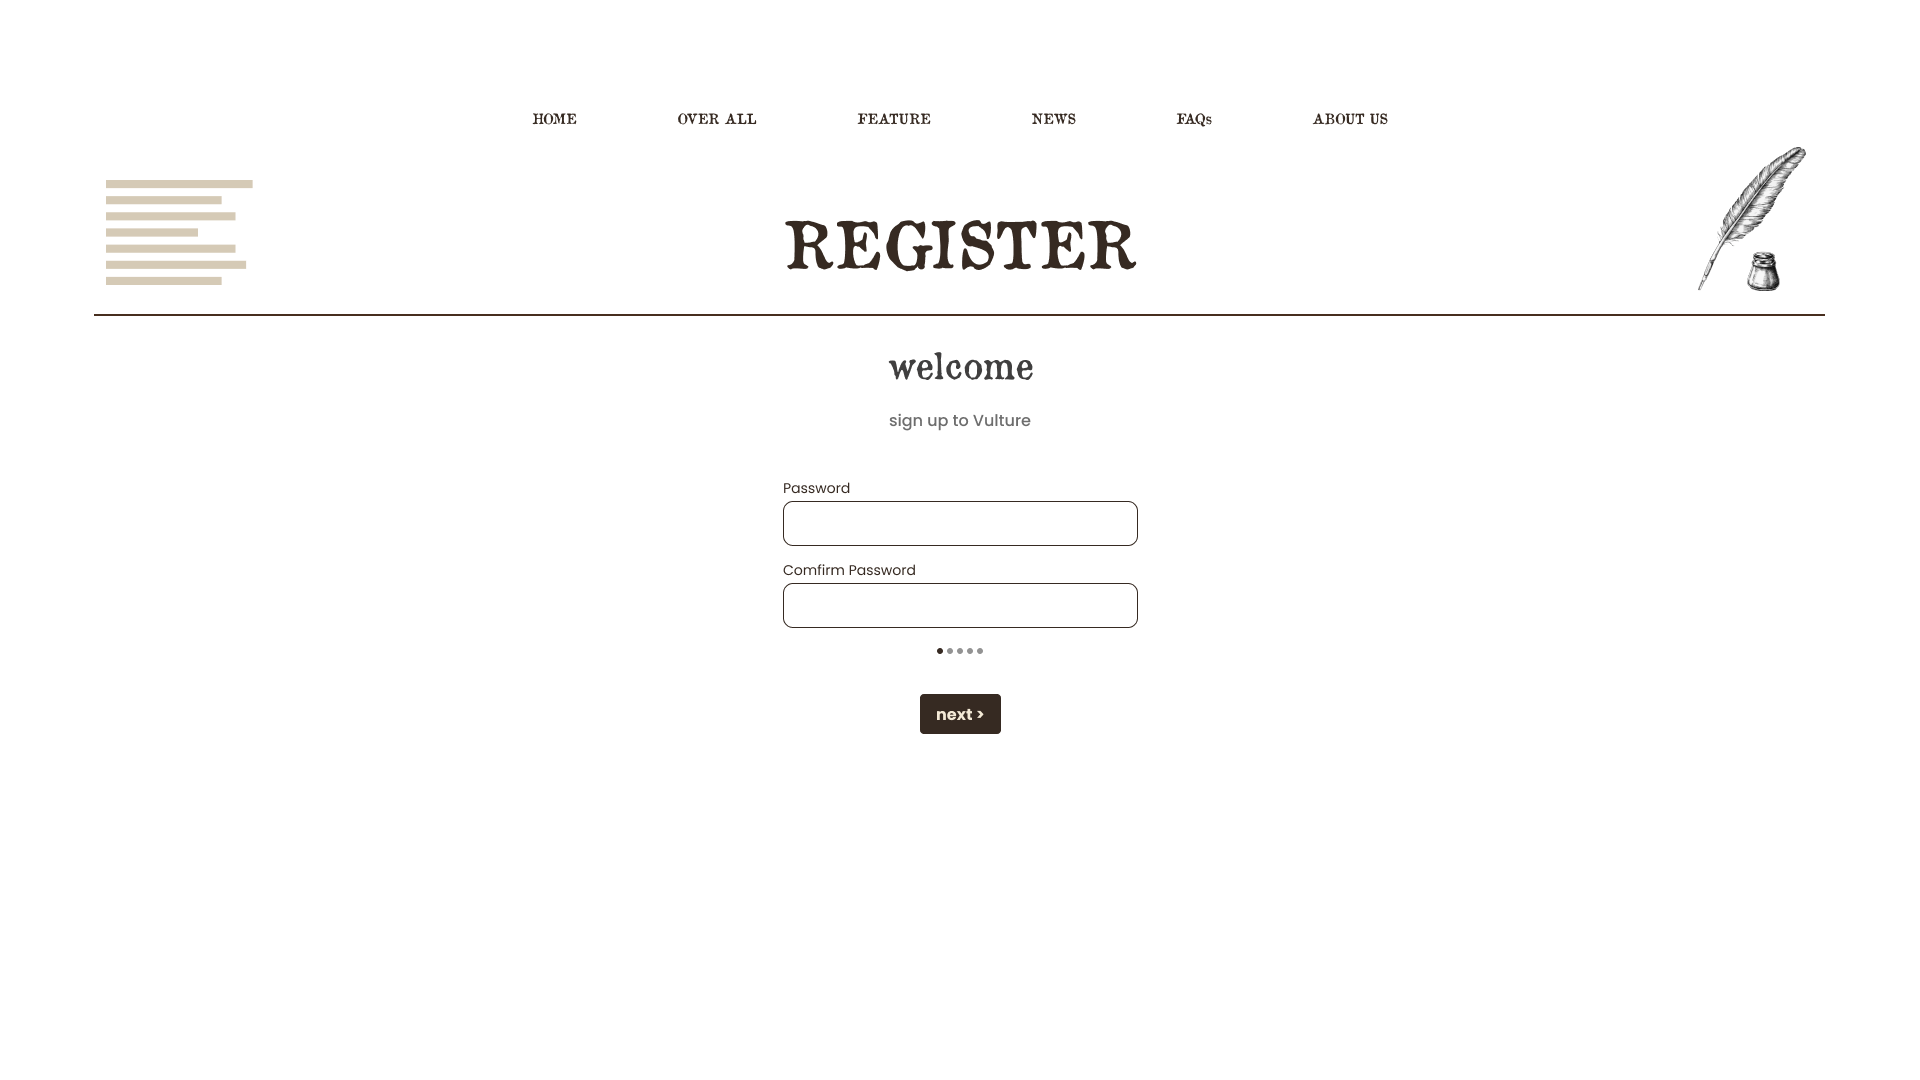
\includegraphics[width=14cm]{./img/project_ui/5.png} 
  \caption{หน้า Register ขั้นตอนกรอก Password}\label{fig:register_password} 
\end{figure}
\hspace*{1cm}เป็นหน้าสำหรับให้ผู้ใช้งานตั้งและยืนยัน Password เพื่อสมัครสมาชิกของเว็บแอปพลิเคชัน AI Platform Thai Content Tagging 
โดยเป็นขั้นตอนถัดจากการกรอก Email (รูปที่:\ref{fig:register}) หากผู้ใช้งานทำการกรอก Password ถูกต้อง เว็บแอปพลิเคชันก็จะพาผู้ใช้งานไปยังหน้า Register ในขั้นตอนถัดไป (รูปที่:\ref{fig:register_name})
\begin{figure}[!ht]\centering
  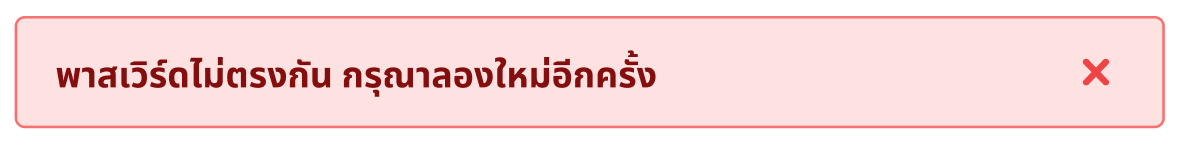
\includegraphics[width=9cm]{./img/project_ui/password.png} 
  \caption{กรอก Password ไม่ตรงกัน}\label{fig:password} 
\end{figure}
\newline\hspace*{1cm}กรณีที่ผู้ใช้งานกรอก Password ไม่ตรงกัน เว็บแอปพลิเคชันจะทำการแจ้งเตือนให้ผู้ใช้งานทราบและให้ผู้ใช้งานกรอก Password ใหม่อีกครั้ง
\begin{figure}[!ht]\centering
  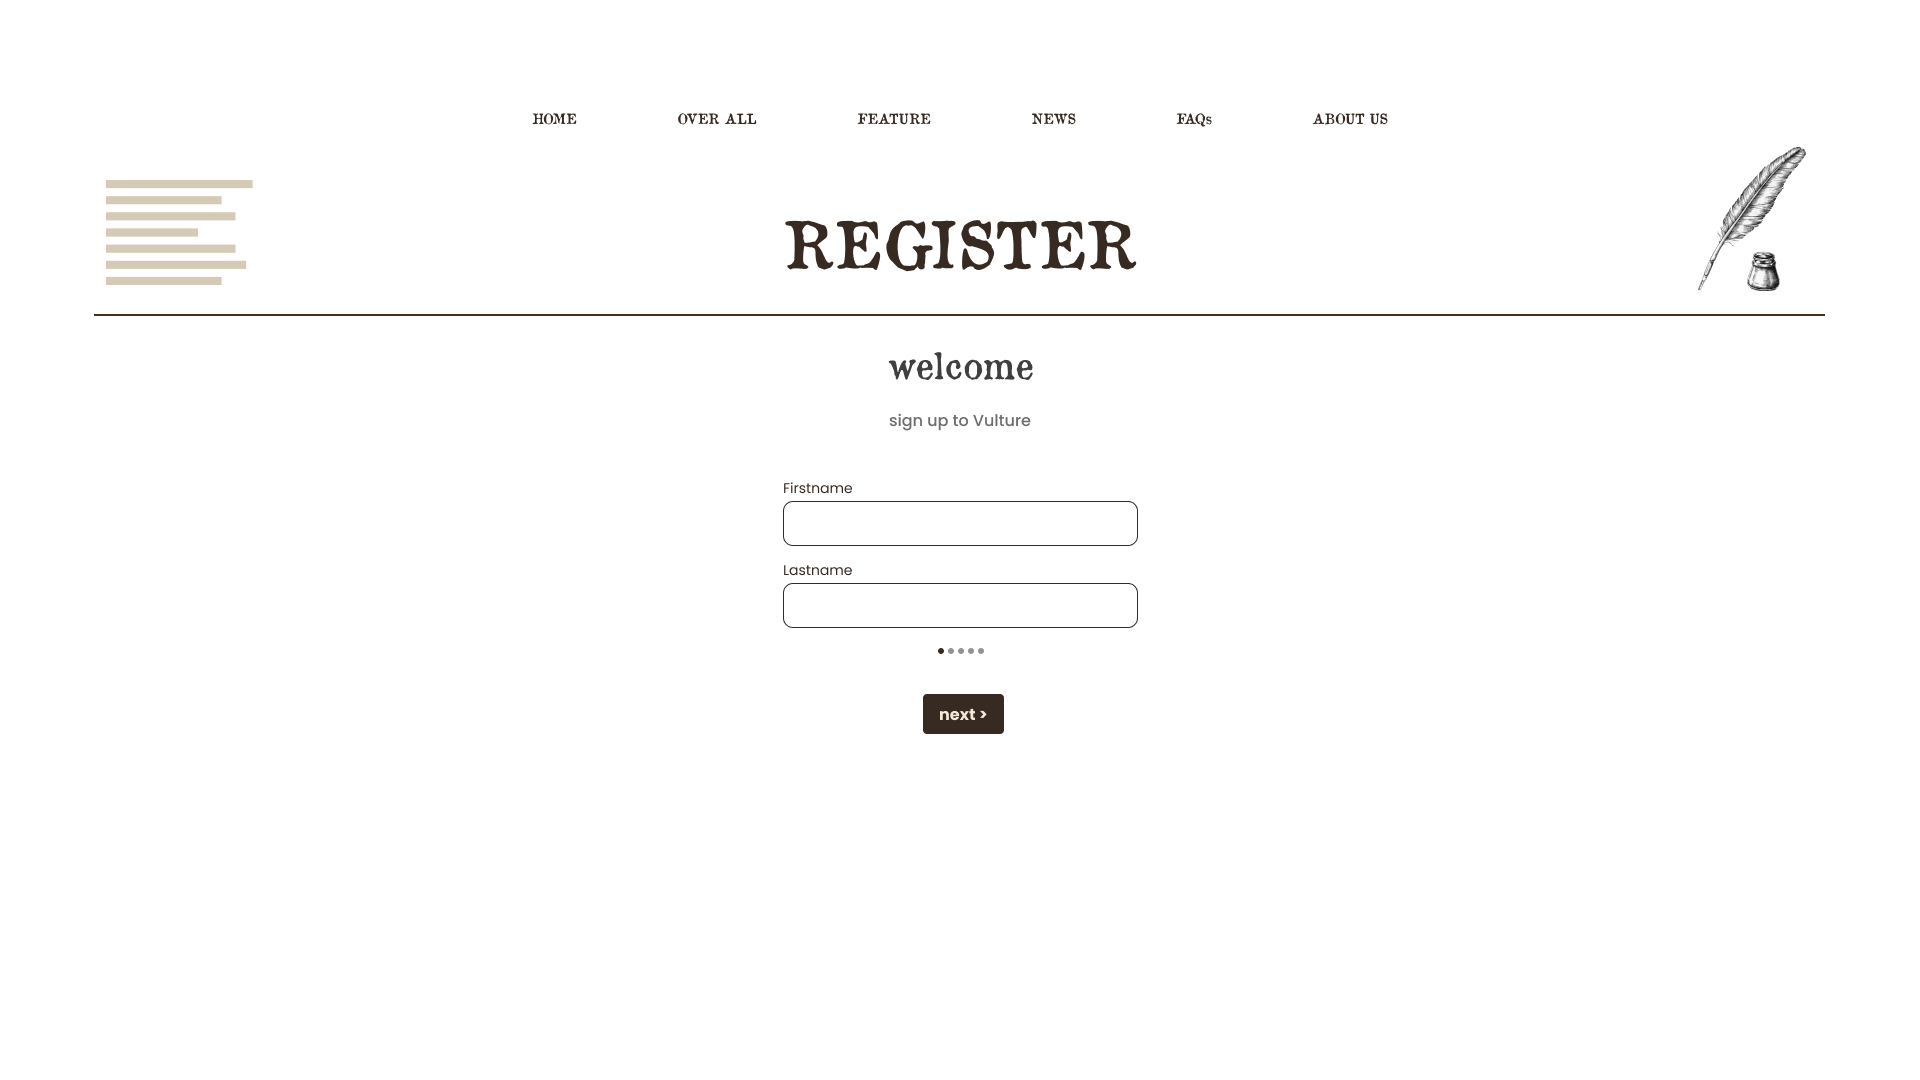
\includegraphics[width=14cm]{./img/project_ui/6.png} 
  \caption{หน้า Register ขั้นตอนกรอกชื่อและนามสกุล}\label{fig:register_name} 
\end{figure} \newpage
\hspace*{1cm}เป็นหน้าสำหรับให้ผู้ใช้งานกรอกชื่อและนามสกุล เพื่อสมัครสมาชิกของเว็บแอปพลิเคชัน AI Platform Thai Content Tagging 
โดยเป็นขั้นตอนถัดจากการกรอก Password (รูปที่:\ref{fig:register_password}) หากผู้ใช้งานทำการกรอกชื่อและนามสกุลถูกต้อง เว็บแอปพลิเคชันก็จะพาผู้ใช้งานไปยังหน้า Register ในขั้นตอนถัดไป (รูปที่:\ref{fig:register_info})
\begin{figure}[!ht]\centering
  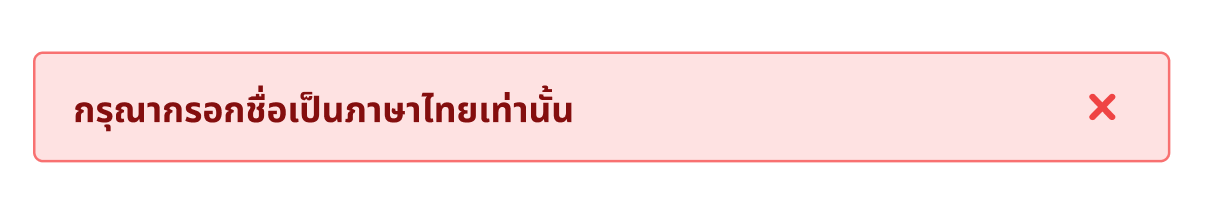
\includegraphics[width=9cm]{./img/project_ui/thaionly.png} 
  \caption{กรอกชื่อและนามสกุลเป็นภาษาอื่น}\label{fig:worngname} 
\end{figure}
\newline\hspace*{1cm}กรณีที่ผู้ใช้งานกรอกชื่อและนามสกุลเป็นภาษาอื่นที่ไม่ใช่ภาษาไทย เว็บแอปพลิเคชันจะทำการแจ้งเตือนให้ผู้ใช้งานทราบและให้ผู้ใช้งานกรอกชื่อและนามสกุลใหม่อีกครั้ง
\begin{figure}[!ht]\centering
  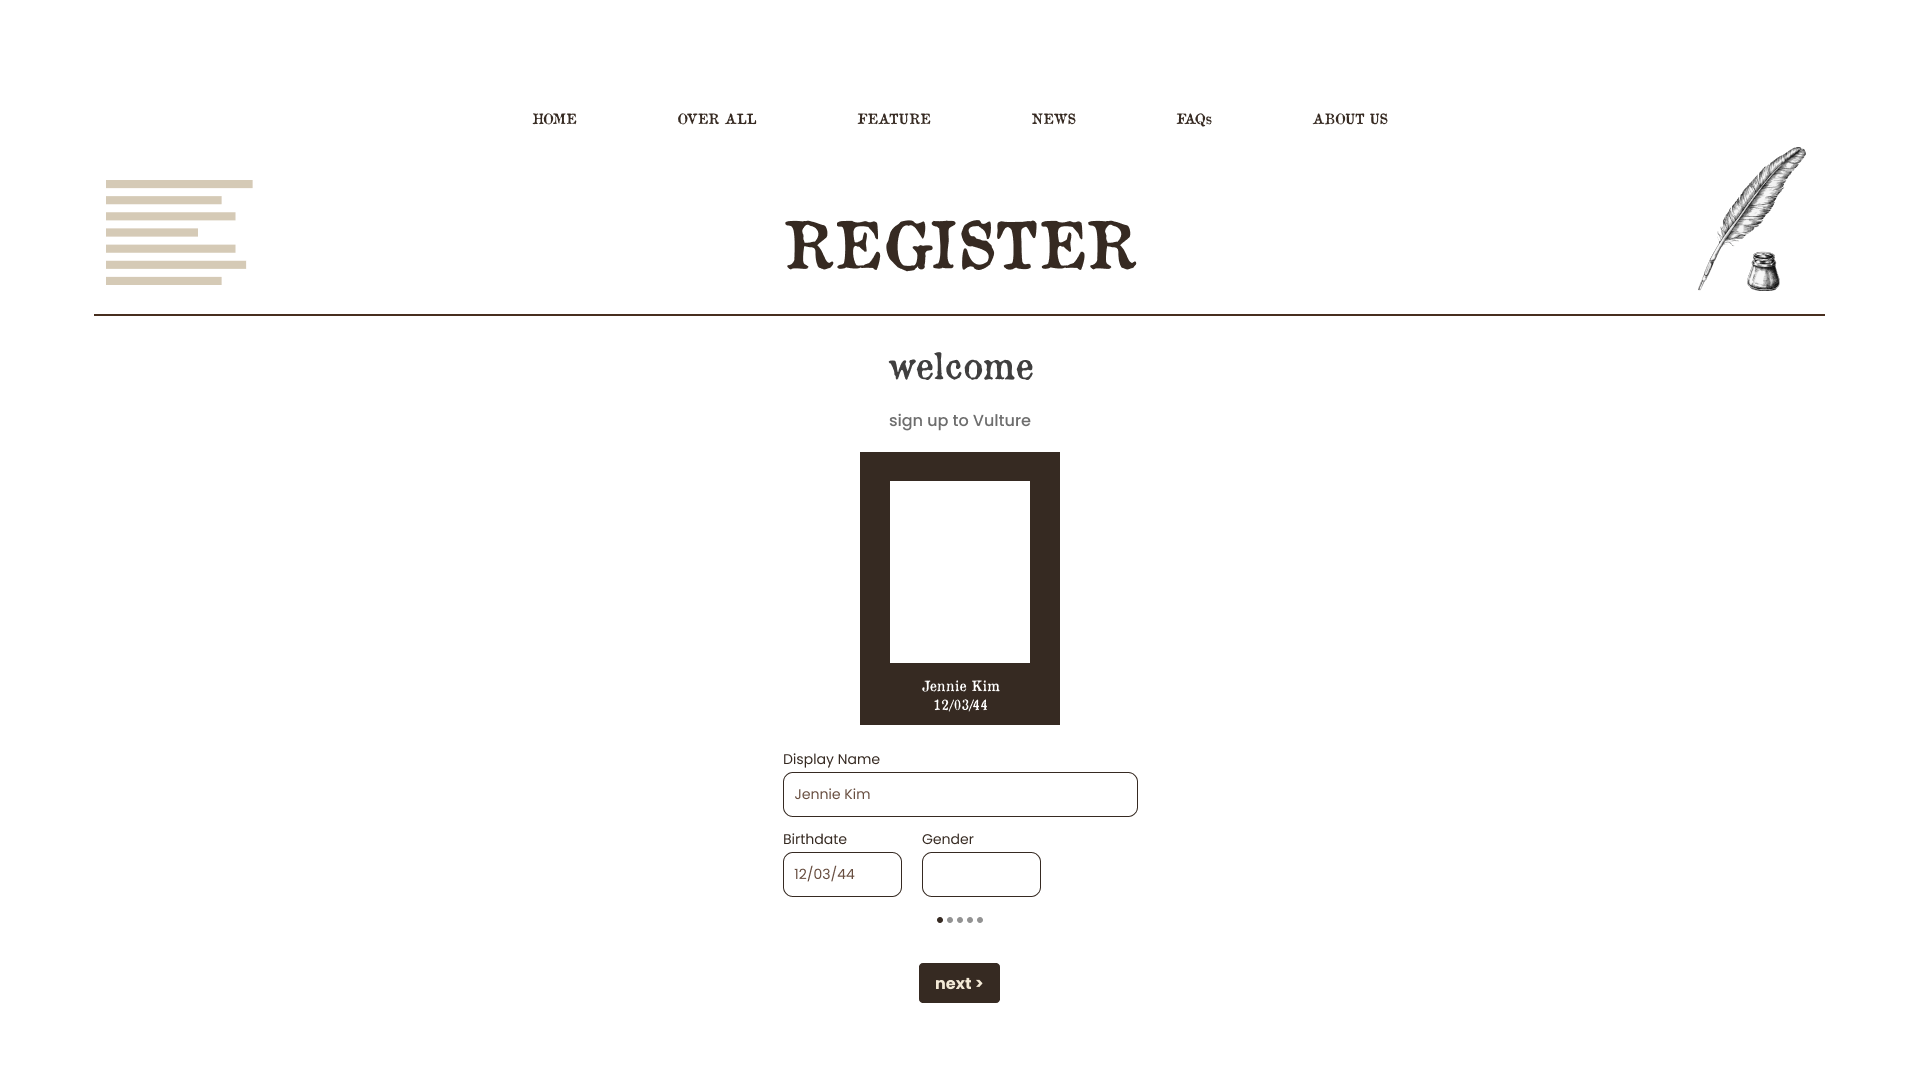
\includegraphics[width=16cm]{./img/project_ui/7.png} 
  \caption{หน้า Register ขั้นตอนกรอกข้อมูลของผู้ใช้งาน}\label{fig:register_info} 
\end{figure}
\newline\hspace*{1cm}เป็นหน้าสำหรับให้ผู้ใช้งานกรอกข้อมูลชื่อเล่น วันเกิด และเพศ พร้อมแนบรูปถ่าย เพื่อสมัครสมาชิกของเว็บแอปพลิเคชัน AI Platform Thai Content Tagging 
โดยเป็นขั้นตอนถัดจากการกรอกชื่อและนามสกุล (รูปที่:\ref{fig:register_name}) หากผู้ใช้งานทำการกรอกข้อมูลครบถ้วน เว็บแอปพลิเคชันก็จะถือว่าผู้ใช้งานทำการสมัครสมาชิกเสร็จสิ้น (รูปที่:\ref{fig:register_already})
\begin{figure}[!ht]\centering
  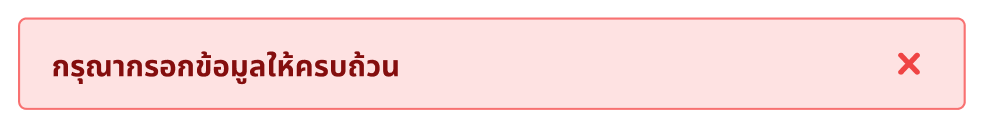
\includegraphics[width=9cm]{./img/project_ui/all_inform.png} 
  \caption{กรอก Password ไม่ตรงกัน}\label{fig:all_inform} 
\end{figure}
\newline\hspace*{1cm}กรณีที่ผู้ใช้งานกรอกข้อมูลไม่ครบถ้วน เว็บแอปพลิเคชันจะทำการแจ้งเตือนให้ผู้ใช้งานทราบและให้ผู้ใช้งานกรอกข้อมูลให้ครบ \newpage
\begin{figure}[!ht]\centering
  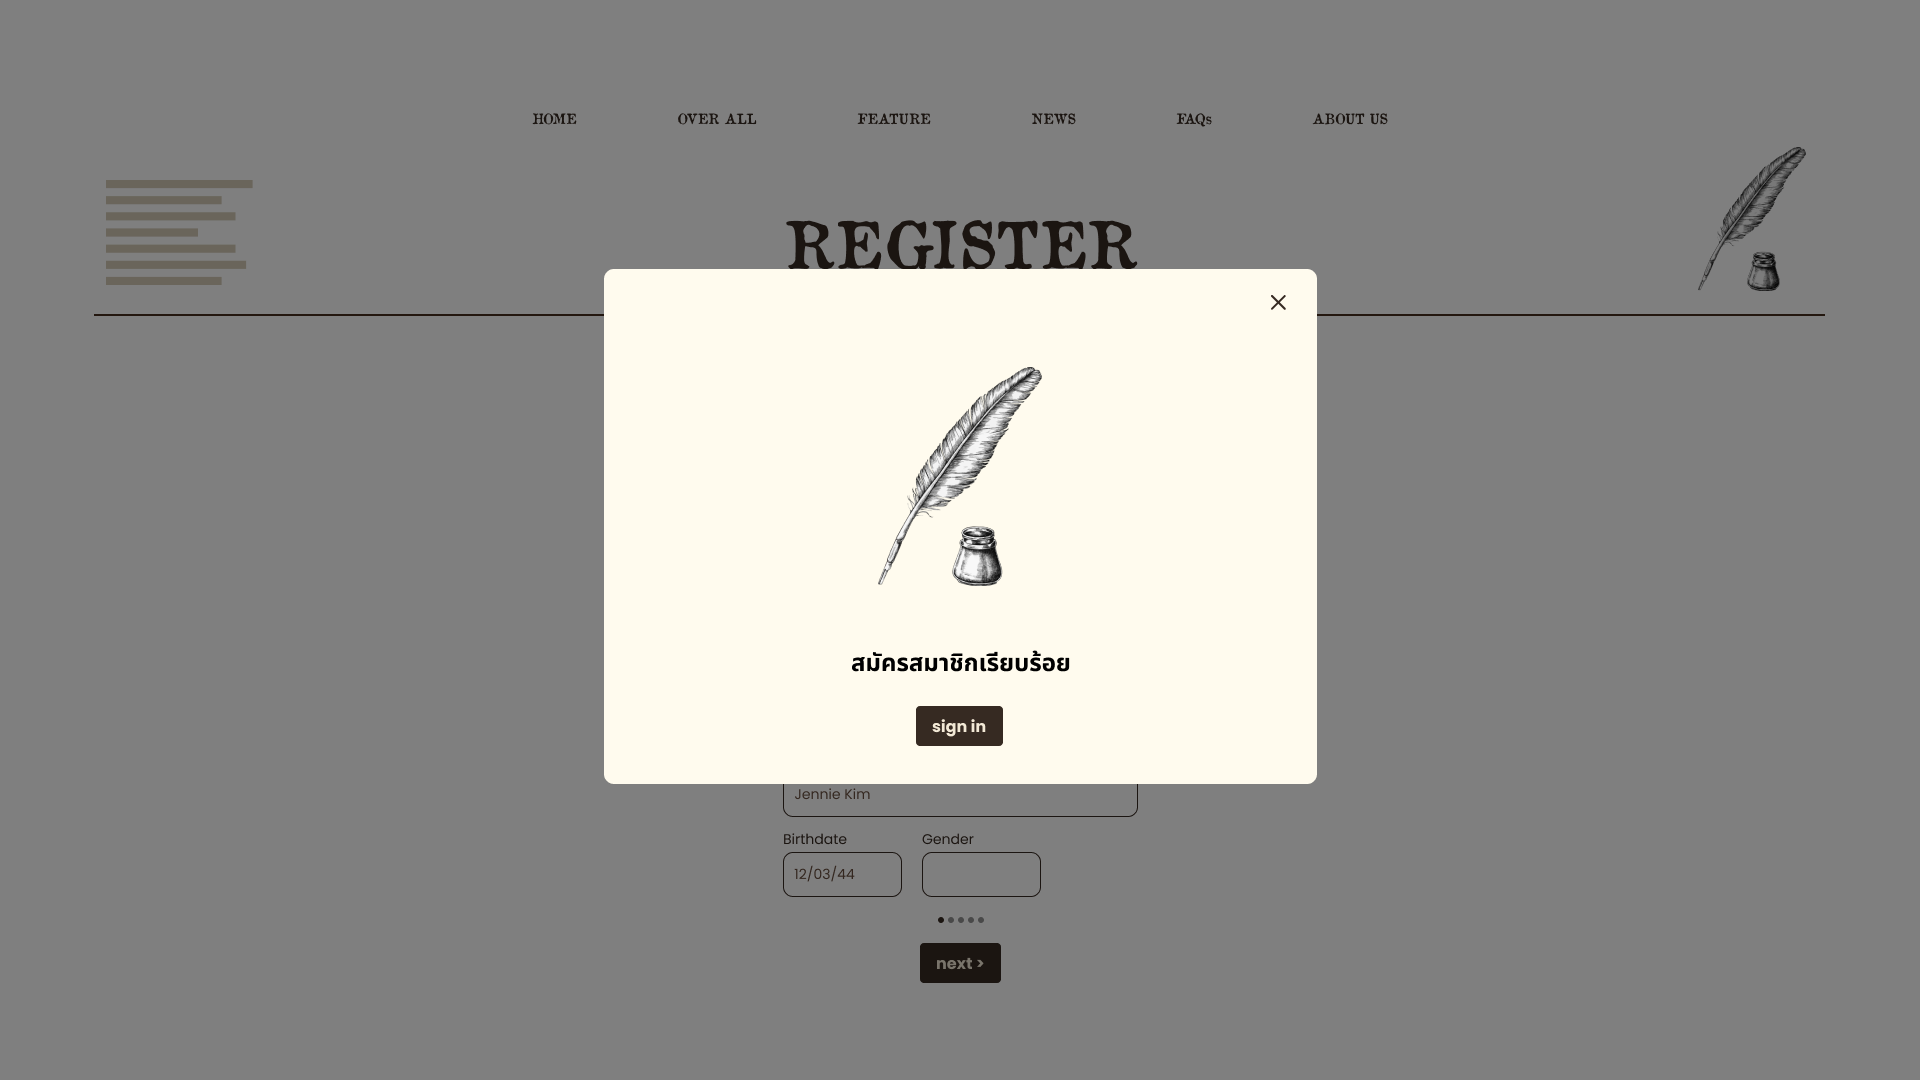
\includegraphics[width=15cm]{./img/project_ui/regis_ready.png} 
  \caption{หน้า Register เมื่อสมัครสมาชิกสำเร็จ}\label{fig:register_already} 
\end{figure}
\hspace*{1cm}เมื่อผู้ใช้งานสมัครสมาชิกของเว็บแอปพลิเคชัน AI Platform Thai Content Tagging เสร็จสิ้นแล้ว 
เว็บแอปพลิเคชันจะทำการแจ้งเตือนว่าผู้ใช้งานได้สมัครสมาชิกเรียบร้อยแล้ว

\subsubsection{หน้า Home}
\begin{figure}[!ht]\centering
  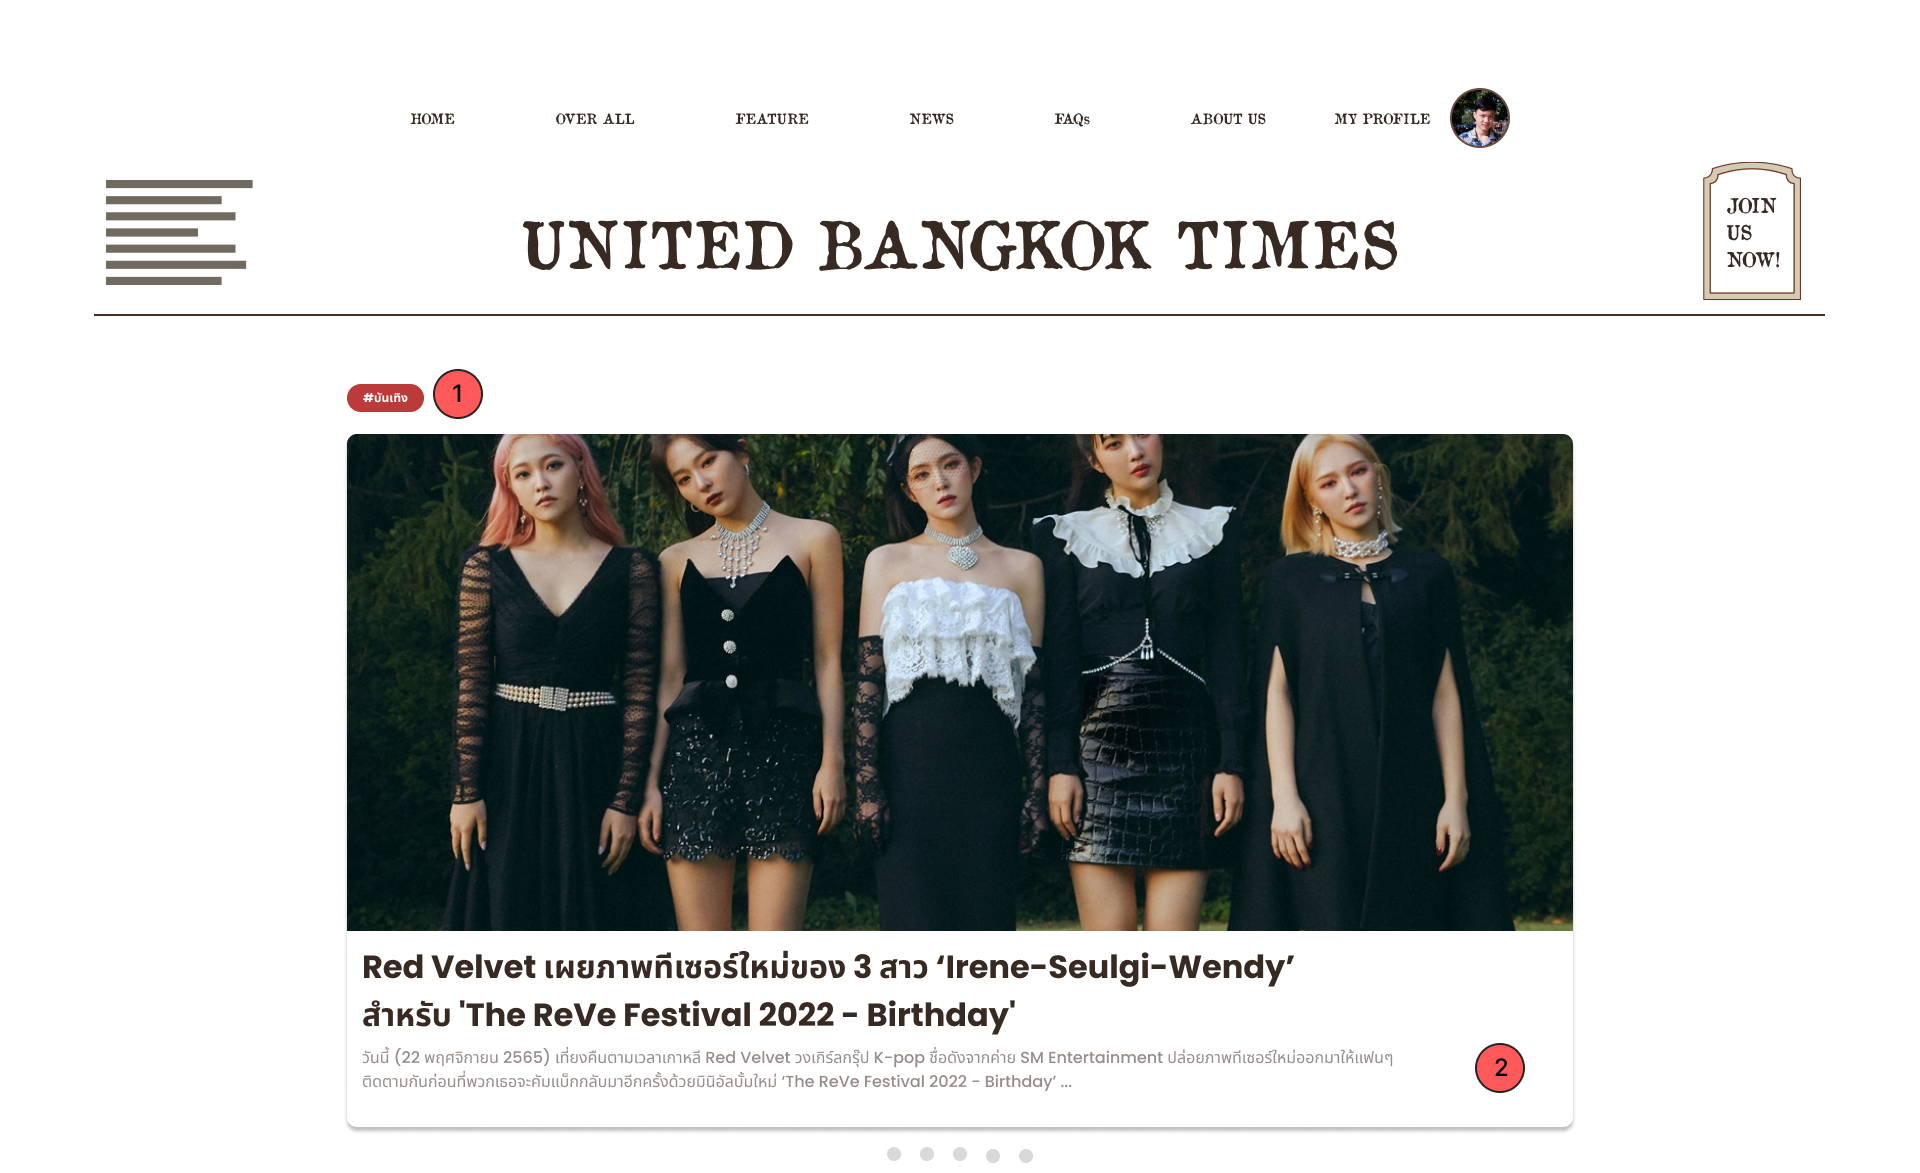
\includegraphics[width=15cm]{./img/project_ui/homepage2.png} 
  \caption{หน้า Home}\label{fig:homepage} 
\end{figure}
\hspace*{1cm}เป็นหน้าที่ผู้ใช้งานทั่วไปและสมาชิกสามารถเข้าถึงได้ สามารถอ่านบทความต่าง ๆ ได้จากหน้า Home Page 
โดยบทความในหน้า Home Page จะถูกจำแนกตามหมวดหมู่ที่เว็บแอปพลิเคชัน AI Platform Thai Content Tagging ได้จัดไว้ \newpage
โดยจากภาพข้างต้น (รูปที่:\ref{fig:homepage}) ก็จะมีอยู่ 2 ส่วนด้วยกัน ได้แก่
\begin{enumerate}
  \item Tag แสดงหมวดหมู่ของเนื้อหาในบทความนั้น ๆ ที่ได้มากจากการวิเคราะห์หมวดหมู่ของบทความโดยเว็บแอปพลิเคชัน AI Platform Thai Content Tagging
  \item เป็นส่วนหัวข้อของบทความ พร้อมกับมีคำอธิบายที่แสดงเนื้อหาภายในบทความคร่าวๆ
\end{enumerate}
\begin{figure}[!ht]\centering
  \includegraphics[width=14cm]{./img/project_ui/homepage3.png} 
  \caption{หน้า Home ส่วนที่เกี่ยวข้องกับการวิเคราะห์หมวดหมู่ของสมาชิก}\label{fig:homepage2} 
\end{figure}
\hspace*{1cm}จากภาพข้างต้น (รูปที่:\ref{fig:homepage2}) จะเป็นส่วนที่ยังคงอยู่ในหน้า Home Page แต่จะเป็นส่วนที่เข้าถึงได้แค่สมาชิกเท่านั้น ผู้ใช้งานทั่วไปไม่สามารถเข้าถึงได้
เนื่องจากเป็นส่วนที่เกี่ยวข้องกับข้อมูลของสมาชิกที่เคยใช้บริการเว็บแอปพลิเคชัน AI Platform Thai Content Tagging ซึ่งจะมีทั้งหมด 3 ส่วน ได้แก่
\begin{itemize}
  \item ส่วนที่ 3 เป็นส่วนที่แสดงตัวอย่างการวิเคราะห์หมวดหมู่ของบทความล่าสุดของสมาชิกที่ได้ทำการร้องขอการวิเคราะห์หมวดหมู่ 
  \item ส่วนที่ 4 เป็นส่วนกรอบโปรไฟล์ของสมาชิก โดยสามารถตรวจสอบว่าบทความที่ทำการส่งไปจัดหมวดหมู่ประมวลผลสำเร็จ รอการประมวลผล หรือล้มเหลวหรือไม่ 
  และจะแสดงบทความก่อน ๆ ที่เคยส่งเพื่อไปวิเคราะห์หมวดหมู่ นอกจากนี้ยังสามารถส่งคำร้องขอเพื่อวิเคราะห์การจัดหมวดหมู่ของบทความ
  และสามารถดูประวัติการส่งคำร้องได้
  \item ส่วนที่ 5 เป็นส่วนที่แสดงหมวดหมู่ที่เว็บแอปพลิเคชัน AI Platform Thai Content Tagging เปิดให้บริการ
\end{itemize}
\begin{figure}[!ht]\centering
  \includegraphics[width=14cm]{./img/project_ui/other_new.png} 
  \caption{หน้า Home ส่วนแสดงข่าวอื่น ๆ เพิ่มเติม}\label{fig:other_new} 
\end{figure}
\hspace*{1cm}ในส่วนที่ 6 จะเป็นส่วนที่แสดงเนื้อหาข่าวอื่น ๆ เพิ่มเติม ซึ่งเป็นส่วนที่ผู้ใช้งานทั่วไปและสมาชิกสามารถเข้าถึงได้ \newpage

\subsubsection{หน้า Analytic}
\begin{figure}[!ht]\centering
  \includegraphics[width=16cm]{./img/project_ui/weblink_1.png} 
  \caption{หน้ากรณีที่สมาชิกต้องการวิเคราะห์หมวดหมู่ของบทความด้วย Web Link}\label{fig:ana_weblink} 
\end{figure}
\hspace*{1cm}เป็นหน้าสำหรับการส่งคำร้องขอเพื่อวิเคราะห์หมวดหมู่ของบทความด้วย Web Link ซึ่งจะมีอยู่ 3 ส่วน ได้แก่
\begin{enumerate}
  \item เป็นส่วนที่ให้สมาชิกเลือกว่าจะส่งคำร้องขอเพื่อวิเคราะห์หมวดหมู่ของบทความด้วยอะไร โดยจะแบ่งเป็น 2 ประเภท คือ 
        การส่งคำร้องขอด้วย Web Link และการส่งคำร้องขอด้วยบทความ โดยสมาชิกสามารถเลือกได้จาก Drop Down
  \item เป็นส่วนสำหรับใส่ Web Link ที่ต้องการวิเคราะห์หมวดหมู่ของบทความ
  \item ปุ่มยืนยันเพื่อส่งคำร้องขอเพื่อวิเคราะห์หมวดหมู่ของบทความด้วย Web Link
\end{enumerate}
\begin{figure}[!ht]\centering
  \includegraphics[width=9cm]{./img/project_ui/linkfail.png} 
  \caption{กรณีที่กรอก Web Link ไม่ถูกต้อง}\label{fig:linkfail} 
\end{figure}
\hspace*{1cm}กรณีที่ผู้ใช้งานกรอก Web Link ไม่ถูกต้อง เว็บแอปพลิเคชันจะทำการแจ้งเตือนให้ผู้ใช้งานทราบและให้ผู้ใช้งานกรอก Web Link ใหม่อีกครั้ง \newpage
\begin{figure}[!ht]\centering
  \includegraphics[width=16cm]{./img/project_ui/content.png} 
  \caption{หน้ากรณีที่สมาชิกต้องการวิเคราะห์หมวดหมู่ของบทความด้วยเนื้อหาในบทความ}\label{fig:raw_content} 
\end{figure}
\hspace*{1cm}เป็นหน้าสำหรับการส่งคำร้องขอเพื่อวิเคราะห์หมวดหมู่ของบทความด้วยเนื้อหาในบทความ ซึ่งจะมีอยู่ 3 ส่วนหลัก ๆ ได้แก่
\begin{enumerate}
  \item เป็นส่วนที่ให้สมาชิกเลือกว่าจะส่งคำร้องขอเพื่อวิเคราะห์หมวดหมู่ของบทความด้วยอะไร โดยจะแบ่งเป็น 2 ประเภท คือ 
        การส่งคำร้องขอด้วย Web Link และการส่งคำร้องขอด้วยบทความ โดยสมาชิกสามารถเลือกได้จาก Drop Down
  \item เป็นส่วนสำหรับใส่หัวข้อของเนื้อหาในบทความที่ต้องการวิเคราะห์หมวดหมู่
  \item เป็นส่วนสำหรับใส่เนื้อหาในบทความที่ต้องการวิเคราะห์หมวดหมู่ของบทความ และจึงกดปุ่มยืนยันเพื่อส่งคำร้องขอเพื่อวิเคราะห์หมวดหมู่ของบทความด้วยเนื้อหาในบทความ
\end{enumerate}
\begin{figure}[!ht]\centering
  \includegraphics[width=9cm]{./img/project_ui/all_inform.png} 
  \caption{กรณีที่กรอกข้อมูลไม่ครบถ้วน}\label{fig:cont_info} 
\end{figure}
\hspace*{1cm}กรณีที่ผู้ใช้งานกรอกข้อมูลไม่ครบถ้วน เว็บแอปพลิเคชันจะทำการแจ้งเตือนให้ผู้ใช้งานทราบและให้ผู้ใช้งานกรอกข้อมูลให้ครบถ้วน \newpage

\subsubsection{หน้า My Ticket}
\begin{figure}[!ht]\centering
  \includegraphics[width=16cm]{./img/project_ui/ticket.png} 
  \caption{หน้า My Ticket}\label{fig:ticket_page} 
\end{figure}
\hspace*{1cm}เป็นหน้าแสดงผลสถานะคำร้องขอเพื่อวิเคราะห์หมวดหมู่ของบทความของสมาชิก ซึ่งจะมีอยู่ 6 ส่วน ได้แก่
\begin{enumerate}
  \item ส่วนแสดงเลขที่อ้างอิงของบทความที่สมาชิกได้ส่งคำร้องเพื่อวิเคราะห์หมวดหมู่ของบทความ
  \item ส่วนแสดงชื่อหัวข้อของบทความ
  \item ส่วนแสดงสถานะดำเนินการของคำร้องขอเพื่อวิเคราะห์หมวดหมู่ของบทความนั้น ๆ โดยมี 3 สถานะด้วยกัน 
        ได้แก่ อยู่ในระหว่างรอประมวลผล (Pending) สำเร็จ (Success) และล้มเหลว (Failed)
  \item ส่วนแสดงหมวดหมู่ที่ได้จากการวิเคราะห์หมวดหมู่ของบทความโดยเว็บแอปพลิเคชัน AI Platform Thai Content Tagging 
        หากล้มเหลวหรือรอดำเนินการจะไม่แสดงผลในส่วนนี้
  \item ส่วนรายละเอียดเพิ่มเติม หากดำเนินการวิเคราะห์หมวดหมู่ของบทความสำเร็จ จะสามารถคลิกดูเพิ่มเติมได้
  \item ส่วนค้นหาคำร้องขอเพื่อวิเคราะห์หมวดหมู่ของบทความของสมาชิก
\end{enumerate} \newpage

\subsubsection{หน้าแสดงผลการวิเคราะห์หมวดหมู่ของบทความ}
\begin{figure}[!ht]\centering
  \includegraphics[width=15cm]{./img/project_ui/12.png} 
  \caption{หน้าแสดงผลการวิเคราะห์หมวดหมู่ของบทความ}\label{fig:result} 
\end{figure} 
\hspace*{1cm}เป็นหน้าแสดงผลการวิเคราะห์หมวดหมู่ของบทความ โดยจะแสดงเลขอ้างอิงของบทความ หัวข้อบทความ เนื้อหาในบทความ 
และหมวดหมู่ที่ได้จากการวิเคราะห์โดยเว็บแอปพลิเคชัน AI Platform Thai Content Tagging 

\subsection{User Interface สำหรับผู้ดูแลระบบ}
\subsubsection{หน้า Home}
\begin{figure}[!ht]\centering
  \includegraphics[width=15cm]{./img/project_ui/admin_home.png} 
  \caption{หน้า Home ของผู้ดูแลระบบ}\label{fig:admin_home} 
\end{figure}
\hspace*{1cm}เป็นหน้าสำหรับผู้ดูแลระบบ เพื่อใช้ในการจัดการรข้อมูลและระบบต่าง ๆ ได้แก่ ข้อมูลของผู้ใช้งานหรือหมวดหมู่ของเนื้อหาในระบบ
โดยในภาพนี้ (รูปที่:\ref{fig:admin_home}) จะมีอยู่ 4 ส่วนด้วยกัน ได้แก่
\begin{enumerate}
  \item เป็นส่วนที่แสดงสถานะต่าง ๆ ได้แก่ จำนวนผู้ใช้งานที่ส่งคำร้องขอในการวิเคราะห์หมวดหมู่ให้กับบทความ จำนวนบทความที่กำลังประมวลผล 
        จำนวนบทความที่ประมวลผลเสร็จเรียบร้อย และจำนวนสมาชิกทั้งหมดภายในระบบ
  \item เป็นส่วนที่แสดงรายละเอียดของบทความต่าง ๆ ที่ผู้ใช้งานได้ส่งคำร้องในการวิเคราะห์เข้ามาในระบบ ซึ่งผู้ดูแลระบบสามารถแก้ไขหรือลบบทความได้ผ่านทางหน้านี้
  \item เมนูสำหรับไปยังหน้าต่าง ๆ ประกอบไปด้วย หน้าหลัก หน้าผู้ใช้งาน และหน้านำเข้าโมเดล ตามลำดับ
  \item ปุ่มสำหรับออกจากระบบ
\end{enumerate}

\subsubsection{หน้า Upload New Model}
\begin{figure}[!ht]\centering
  \includegraphics[width=15cm]{./img/project_ui/admin_up.png} 
  \caption{หน้า Upload โมเดลใหม่}\label{fig:admin_upload} 
\end{figure}
\hspace*{1cm}เป็นหน้าสำหรับผู้ดูแลระบบ เพื่อใช้ในอัพเดทโมเดลเข้าไปใหม่ในระบบ
โดยในภาพนี้ (รูปที่:\ref{fig:admin_upload}) จะมีอยู่ 2 ส่วนด้วยกัน ได้แก่
\begin{enumerate}
  \item ผู้ดูแลระบบสามารถอัพเดทโมเดลผ่านทางเว็บแอปพลิเคชันด้วยการเลือกที่ปุ่มอัพโหลด ซึ่งสามารถอัพโหลดได้เพียงแค่นามสกุลไฟล์ joblib เท่านั้น
  \item เป็นส่วนที่แสดงให้เห็นสถานะการอัพเดทโมเดล โดยจะสามารถเลือกที่ปุ่ม "Go to pipeline" เพื่อดูรายละเอียดเพิ่มเติมได้
\end{enumerate}

\section{Class Diagram}
  \hspace{1cm}การออกแบบ Class Diagram จะออกแบบให้มีความ Loose Coupling โดยจะมีการทำ Interface และ Dependency Injection ในการเชื่อมต่อกันระหว่างคลาสต่าง ๆ
  เพื่อให้โค้ดสามารถทดสอบได้ง่าย
\begin{figure}[!ht]\centering
  \includegraphics[width=15cm]{./img/class_dia.png} 
  \caption{Class Diagram ของระบบ}\label{fig:class_diagram} 
\end{figure} 
\newpage

\section{การออกแบบการทดลอง}
\subsection{User Evaluation}
\hspace*{1cm}ทดสอบเว็ปแอปพลิเคชันกับผู้ใช้งานจำนวน 20 คน โดยเก็บข้อมูลทั้งการตอบสนองต่อความต้องการและประสบการณ์การใช้งานของผู้ใช้งาน 
เพื่อเก็บรวบรวมเป็นข้อมูลสำหรับนำไปพัฒนาปรับปรุงเว็บแอปพลิเคชันให้สามารถตอบสนองความต้องการได้ดียิ่งขึ้น
\subsection{Application Evaluation}
\hspace*{1cm}การประเมินผล Application จะประเมินใน 2 รูปแบบ ได้แก่
  \begin{enumerate}
    \item การประเมินความสามารถของ Application นั้น ๆ ว่าสามารถทำฟังก์ชันไหนได้บ้าง เช่น สามารถทำนายหมวดหมู่ของบทความได้ สามารถแสดงผลการวิเคราะห์หมวดหมู่ของบทความได้
    \item การประเมินประสิทธิภาพของ Application ว่าสามารถทำงานได้ดีแค่ไหน เช่น จำนวนข้อมูลที่สามารถรองรับได้ ความเร็วในการทำงาน ความแม่นยำในการทำงาน
  \end{enumerate}
\subsection{Artificial Intelligence Evaluation}
\hspace*{1cm}การประเมินผลติดตามการใช้งาน Artificial Intelligence ก็มีส่วนสำคัญในการพัฒนา Artificial Intelligence ให้มีความแม่นยำมากยิ่งขึ้น 
ซึ่งจำเป็นต้องใช้ข้อมูลที่ถูกต้องเป็นจำนวนมาก สำหรับการทดสอบความแม่นยำของ Artificial Intelligence เพื่อให้ Artificial Intelligence สามารถใช้เป็นแหล่งข้อมูลอ้างอิงและวิเคราะห์ผลได้แม่นยำมากยิ่งขึ้น
กล่าวคือต้องใช้บทความที่มีการจัดหมวดหมู่อย่างถูกต้องจำนวนมาก เพื่อนำบทความนั้นมาทดสอบกับ Artificial Intelligence และเปรียบเทียบผลลัพธ์ว่าตรงตามหมวดหมู่ของบทความที่เตรียมมาหรือไม่
โดยจะใช้ตัววัดผลคือ ค่า Accuracy, Precision, Recall, F1 Score และ Loss Function ในการวัดประสิทธิภาพของ Artificial Intelligence


%%%%%%%%%%%%%%%%%%%%%%%%%%%%%%%%%%%%%%%%%%%%%%%%%%%%%%%%%%%%%%
%%%%%%%%%%%%%%%%%%%% Experiments %%%%%%%%%%%%%%%%%%%%%%%%%%%%%
%%%%%%%%%%%%%%%%%%%%%%%%%%%%%%%%%%%%%%%%%%%%%%%%%%%%%%%%%%%%%%%
\chapter{ผลการดำเนินงาน}

  \section{การเก็บข้อมูล}
    \hspace{1cm}ในส่วนของการเก็บข้อมูลสำหรับการพัฒนาโมเดล จะได้ผลลัพธ์ดังนี้

    \hspace{1cm}การเก็บ URL จากหน้าเว็บไซต์ ซึ่งในขั้นตอนนี้สามารถทำได้ 2 วิธี ได้แก่ วิธีแรก คือ การบันทึกหน้าเว็บไซต์ที่มีข้อมูลบทความจำนวนมาก นำมาอ่านข้อมูล HTML 
    แล้วจึงเก็บ URL ของบทความต่าง ๆ และวิธีที่สอง คือ การอ่าน URL ผ่าน Request โดยเว็บไซต์จะทำการส่ง Request ร้องขอเพื่อดูบทความเพิ่มเติม 
    เมื่อได้ URL มาครบตามที่ต้องการแล้ว จะทำการดึงข้อมูลเป็นไฟล์ HTML จาก URL ที่เก็บมาจากหน้าเว็บไซต์ 
    จากนั้นทำการเข้าถึงไฟล์ HTML ที่ได้จาก URL ที่เก็บมาจากหน้าเว็บไซต์และทำการดึงเนื้อหาบทความด้วยการใช้ Python BeautifulSoup มาเก็บไว้ 
    เพื่อเป็นชุดข้อมูลสำหรับพัฒนาโมเดล ได้ผลลัพธ์ดังรูปที่ \ref{fig:data_thai}
    \begin{figure}[!ht]\centering
      \includegraphics[width=0.9\textwidth]{./img/data_col_thai.png}
      \caption{ตัวอย่างการดึงเนื้อหาบทความจากไฟล์ HTML ด้วยการใช้ Python BeautifulSoup}\label{fig:data_thai}
    \end{figure}

    \hspace{1cm}ทำการแปลเนื้อหาที่ได้จากรูปภาพที่ \ref{fig:data_thai} ซึ่งเป็นเนื้อหาที่เป็นภาษาไทยให้กลายเป็นภาษาอังกฤษด้วยการใช้ Translator Service
    เพื่อใช้สำหรับการพัฒนาโมเดลที่ใช้ชุดข้อมูลเป็นภาษาอังกฤษ ได้ผลลัพธ์ดังรูปที่ \ref{fig:data_thai}
    \begin{figure}[!ht]\centering
      \includegraphics[width=0.9\textwidth]{./img/data_col_eng.png}
      \caption{ตัวอย่างการแปลเนื้อหาจากภาษาไทยเป็นภาษาอังกฤษ}\label{fig:data_eng}
    \end{figure}
    \newpage

  \section{การออกแบบโมเดลสำหรับวิเคราะห์หมวดหมู่ของเนื้อหาในบทความต่าง ๆ}
    \subsection{การเตรียมข้อมูลสำหรับการพัฒนาโมเดล}
      \hspace{1cm}ข้อมูลที่ใช้ในการพัฒนาโมเดลจะมีทั้งหมด 2 รูปแบบด้วยกัน ได้แก่ ชุดข้อมูลที่มีเนื้อหาเป็นภาษาไทยและชุดข้อมูลวที่มีเนื้อหาเป็นภาษาอังกฤษ
      ชุดข้อมูลที่มีเนื้อหาเป็นภาษาไทยจะมีทั้งหมด 9,000 ชุด และชุดข้อมูลที่มีเนื้อหาเป็นภาษาอังกฤษจะมีทั้งหมด 9,000 ชุด ซึ่งมีลักษณะข้อมูลเป็นไฟล์ Text
      และมีหมวดหมู่กำกับในแต่ละชุดข้อมูล โดยมีรายละเอียดดังนี้

      \begin{longtable}[!ht]{p{0.15\linewidth}m{0.45\linewidth}}
        \caption{ตารางชุดข้อมูลข่าวที่มีเนื้อหาเป็นภาษาไทย}
        \label{tbl:new_th}\\
        \hhline{==}
        \multicolumn{1}{c}{\textbf{หมวดหมู่}} & \multicolumn{1}{c}{\textbf{จำนวนชุดข้อมูลข่าว}} \\ \hline
        \endhead
        %
        อาชญากรรม                              & \multicolumn{1}{c}{1,500}                        \\ %\hline
        กีฬา                                   & \multicolumn{1}{c}{1,500}                         \\ %\hline
        การเมือง                               & \multicolumn{1}{c}{1,500}                          \\ %\hline
        เศรษฐกิจ                                 & \multicolumn{1}{c}{1,500}                          \\ %\hline
        บันเทิง                                & \multicolumn{1}{c}{1,500}                          \\ %\hline
        เทคโนโลยี                              & \multicolumn{1}{c}{1,500}                          \\ \hline
        \textbf{รวม}                           & \multicolumn{1}{c}{\textbf{9,000}}                        \\ \hhline{==}
      \end{longtable}

      \begin{figure}[!ht]\centering
        \includegraphics[width=13cm]{./img/news_th.png}
        \caption{ตัวอย่างชุดข้อมูลข่าวที่มีเนื้อหาเป็นภาษาไทย}\label{fig:new_th}
      \end{figure}

      \begin{longtable}[!ht]{p{0.15\linewidth}m{0.45\linewidth}|}
        \caption{ตารางชุดข้อมูลข่าวที่มีเนื้อหาเป็นภาษาอังกฤษ}
        \label{tbl:new_eng}\\
        \hhline{==}
        \multicolumn{1}{c}{\textbf{หมวดหมู่}} & \multicolumn{1}{c}{\textbf{จำนวนชุดข้อมูลข่าว}} \\ \hline
        \endhead
        %
        อาชญากรรม                              & \multicolumn{1}{c}{1,500}                        \\ %\hline
        กีฬา                                   & \multicolumn{1}{c}{1,500}                         \\ %\hline
        การเมือง                               & \multicolumn{1}{c}{1,500}                          \\ %\hline
        เศรษฐกิจ                                 & \multicolumn{1}{c}{1,500}                          \\ %\hline
        บันเทิง                                & \multicolumn{1}{c}{1,500}                          \\ %\hline
        เทคโนโลยี                              & \multicolumn{1}{c}{1,500}                          \\ \hline
        \textbf{รวม}                           & \multicolumn{1}{c}{\textbf{9,000}}                        \\ \hhline{==}
      \end{longtable}
      \newpage

      \begin{figure}[!ht]\centering
        \includegraphics[width=13cm]{./img/news_eng.png}
        \caption{ตัวอย่างชุดข้อมูลข่าวที่มีเนื้อหาเป็นภาษาอังกฤษ}\label{fig:new_eng}
      \end{figure}

      \hspace{1cm}นอกจากนี้คณะผู้จัดทำได้ทำการแบ่งชุดข้อมูลออกเป็น 2 ส่วน ส่วนแรกสำหรับการพัฒนาโมเดลและส่วนที่สองสำหรับการประเมินโมเดล
      ซึ่งจะแบ่งชุดข้อมูลแต่ละรูปแบบออกเป็นอัตราส่วน 8:2 (ชุดข้อมูลสำหรับการพัฒนาโมเดล : ชุดข้อมูลสำหรับการประเมินโมเดล)
      โดยมีรายละเอียดดังนี้

      \begin{longtable}[!ht]{lcc}
        \caption{ตารางชุดข้อมูลที่มีเนื้อหาเป็นภาษาไทยสำหรับใช้พัฒนาและทดสอบโมเดล}
        \label{tbl:new_thai_traintest}\\
        \hhline{===}
        \multicolumn{1}{c}{\textbf{หมวดหมู่}} &
          \textbf{\begin{tabular}[c]{@{}c@{}}จำนวนชุดข้อมูล\\ สำหรับพัฒนาโมเดล\end{tabular}} &
          \textbf{\begin{tabular}[c]{@{}c@{}}จำนวนชุดข้อมูล\\ สำหรับประเมินโมเดล\end{tabular}} \\ \hline
        \endhead
        %
        อาชญากรรม    & 1,200 & 300 \\ %\hline
        กีฬา         & 1,200 & 300 \\ %\hline
        การเมือง     & 1,200  & 300 \\ %\hline
        เศรษฐกิจ       & 1,200  & 300  \\ %\hline
        บันเทิง      & 1,200  & 300  \\ %\hline
        เทคโนโลยี    & 1,200  & 300  \\ \hline
        \textbf{รวม} & \textbf{7,200} & \textbf{1,800} \\ \hhline{===}
      \end{longtable} 

      \begin{longtable}[!ht]{lcc}
        \caption{ตารางชุดข้อมูลที่มีเนื้อหาเป็นภาษาอังกฤษสำหรับใช้พัฒนาและทดสอบโมเดล}
        \label{tbl:new_eng_traintest}\\
        \hhline{===}
        \multicolumn{1}{c}{\textbf{หมวดหมู่}} &
          \textbf{\begin{tabular}[c]{@{}c@{}}จำนวนชุดข้อมูล\\ สำหรับพัฒนาโมเดล\end{tabular}} &
          \textbf{\begin{tabular}[c]{@{}c@{}}จำนวนชุดข้อมูล\\ สำหรับประเมินโมเดล\end{tabular}} \\ \hline
        \endhead
        %
        อาชญากรรม    & 1,200 & 300 \\ %\hline
        กีฬา         & 1,200 & 300 \\ %\hline
        การเมือง     & 1,200  & 300 \\ %\hline
        เศรษฐกิจ       & 1,200  & 300  \\ %\hline
        บันเทิง      & 1,200  & 300  \\ %\hline
        เทคโนโลยี    & 1,200  & 300  \\ \hline
        \textbf{รวม} & \textbf{7,200} & \textbf{1,800} \\ \hhline{===}
      \end{longtable} 

      \hspace{1cm}การเตรียมข้อมูลสำหรับการพัฒนาโมเดล จะมีการทำความความสะอาดข้อมูลก่อนอย่างการลบอักขระที่ไม่จำเป็น ลบตัวเลข หรือช่องว่าง
      เพื่อเป็นการลบการรบกวนของข้อมูล จากนั้นจึงทำการแบ่งคำสำหรับลบ Stop word และปรับคำให้อยู่ในรูปแบบที่เป็นบรรทัดฐาน เพื่อลดความซ้ำซ้อนของข้อมูล
      แล้วจึงนำมาเรียบเรียงต่อกันเป็นประโยคใหม่ โดยนำหัวข้อและเนื้อหารวมกันเป็นบทความเดียว ทำให้สามารถดึง Feature ออกจากข้อมูลได้อย่างมีประสิทธิภาพมากขึ้น
      \newpage
      \begin{figure}[!ht]\centering
        \includegraphics[width=7cm]{./img/new_th_train.png}
        \caption{ตัวอย่างชุดข้อมูลที่มีเนื้อหาเป็นภาษาไทยที่ผ่านการเตรียมข้อมูลแล้ว}\label{fig:new_th_train}
      \end{figure}

      \begin{figure}[!ht]\centering
        \includegraphics[width=7cm]{./img/news_eng_train.png}
        \caption{ตัวอย่างชุดข้อมูลที่มีเนื้อหาเป็นภาษาอังกฤษที่ผ่านการเตรียมข้อมูลแล้ว}\label{fig:new_eng_train}
      \end{figure}

    \subsection{Exploratory Data Analysis}
      \subsubsection{ชุดข้อมูลที่มีเนื้อหาเป็นภาษาไทย}
        \hspace{1cm}จากการสำรวจชุดข้อมูลที่มีเนื้อหาเป็นภาษาไทยทั้งหมด 9,000 ชุด พบว่า แต่ละชุดข้อมูลมีการกระจายตัวของขนาดของข้อมูล \newline ดังนี้
        \begin{figure}[!ht]\centering
          \includegraphics[width=\textwidth]{./img/thai_stat/hist_all_word.png}
          \caption{การกระจายตัวของจำนวนคำในแต่ละชุดข้อมูลที่มีเนื้อหาเป็นภาษาไทย}\label{fig:thai_hist}
        \end{figure}
        \begin{longtable}[!ht]{ccccccc}
          \caption{ตารางแสดงค่าทางสถิติของจำนวนคำในเนื้อหาที่เป็นภาษาไทยทั้งหมดหลังทำความสะอาดข้อมูล}
          \label{tbl:thai_stat_all}\\
          % \hline
          \hhline{=======}
          \textbf{Mean} & \textbf{STD} & \textbf{Min} & \textbf{Q1} & \textbf{Q2} & \textbf{Q3} & \textbf{Max}\\ \hline
          \endhead
          %
          239.14 & 175.10 & 6.00 & 139.00 & 195.00 & 286.00 & 3356.00  \\ \hhline{=======}%\hline
        \end{longtable}
        \hspace{1cm}จะเห็นได้ว่าการกระจายตัวของจำนวนคำในแต่ละชุดข้อมูลที่มีเนื้อหาเป็นภาษาไทย มีการกระจายตัวแบบเบ้ขวาและมี Outlier (รูปที่:\ref{fig:thai_hist}) 
        ดังนั้นค่าเฉลี่ยของจำนวนคำในชุดข้อมูลจึงมากกว่าค่ากลางของจำนวนคำในชุดข้อมูล และเมื่อดูการกระจายตัวประกอบกับค่าทางสถิติของจำนวนคำในเนื้อหาทั้งหมด
        (ตารางที่:\ref{tbl:thai_stat_all}) พบว่า จำนวนคำในชุดข้อมูลที่มีเนื้อหาเป็นภาษาไทยส่วนใหญ่จะมีค่าอยู่ที่ 140-290 คำ โดยจำนวนคำที่น้อยที่สุดในชุดข้อมูล คือ 6 คำ
        และจำนวนคำที่มากที่สุดในชุดข้อมูล คือ 3,356 คำ
        
        \begin{longtable}[!ht]{lccccccc}
          \caption{ตารางแสดงค่าทางสถิติของจำนวนคำในเนื้อหาที่เป็นภาษาไทยของแต่ละหมวดหมู่หลังทำความสะอาดข้อมูล}
          \label{tbl:thai_stat}\\
          \hhline{========}
          \multicolumn{1}{c}{\textbf{หมวดหมู่}} & \textbf{Mean} & \textbf{STD} & \textbf{Min} & \textbf{Q1} & \textbf{Q2} & \textbf{Q3} & \textbf{Max}\\ \hline
          \endhead
          %
          อาชญากรรม    & 294.51 & 182.57 & 71.00 & 193.00 & 257.00 & 343.00 & 2006.00  \\ %\hline
          กีฬา          & 239.04 & 222.40 & 21.00 & 129.00 & 173.50 & 271.00 & 3356.00  \\ %\hline
          การเมือง       & 227.62 & 147.87 & 12.00 & 140.75 & 196.00 & 276.00 & 2174.00  \\ %\hline
          เศรษฐกิจ         & 190.63 & 127.83  & 21.00 & 110.00 & 160.00 & 235.25 & 762.00  \\ %\hline
          บันเทิง        & 233.04 & 167.31 & 6.00 & 129.00 & 173.00 & 279.25 & 1327.00  \\ %\hline
          เทคโนโลยี     & 249.99 & 171.35 & 12.00 & 163.00 & 206.00 & 291.00 & 3209.00  \\ \hhline{========}
        \end{longtable}
        \begin{figure}[!ht]\centering
          \includegraphics[width=\textwidth]{./img/thai_stat/boxplot_all.png}
          \caption{ลักษณะของจำนวนคำในเนื้อหาที่เป็นภาษาไทยของแต่ละหมวดหมู่หลังทําความสะอาดข้อมูล}\label{fig:thai_boxplot}
        \end{figure}
        \hspace{1cm}เนื่องจากในแต่หมวดหมู่ของชุดข้อมูลมีขนาดของข้อมูลแตกต่างกัน ซึ่งในชุดข้อมูลที่มีเนื้อหาเป็นภาษาไทยจะมีทั้งหมด 6 หมวดหมู่ด้วยกัน
        ดังนั้นจึงต้องมีการสำรวจการกระจายตัวของขนาดของข้อมูลในแต่ละหมวดหมู่ ซึ่งจากตารางที่ \ref{tbl:thai_stat} และรูปภาพที่ \ref{fig:thai_boxplot}
        พบว่า จำนวนคำของเนื้อหาในหมวดหมู่อาชญากรรมส่วนใหญ่จะมีค่ามากกว่าหมวดหมู่อื่น ในขณะที่จำนวนคำของเนื้อหาในหมวดหมู่เศรษฐกิจส่วนใหญ่จะมีค่าน้อยกว่าหมวดหมู่อื่น
        นอกจากนี้ยังพบว่า จำนวนคำของชุดข้อมูลในหมวดหมู่กีฬามีการกระจายตัวของกลุ่มข้อมูลสูงสุดและจำนวนคำของชุดข้อมูลในหมวดหมู่เศรษฐกิจมีการกระจายตัวของกลุ่มข้อมูลต่ำสุด
        ซึ่งสังเกตได้จากค่า STD ในตารางที่ \ref{tbl:thai_stat}
        \newpage
        \begin{figure}[!ht]\centering
          \includegraphics[width=0.7\textwidth]{./img/thai_stat/crime_bar.png}
          \caption{10 คำที่พบได้มากที่สุดในชุดข้อมูลที่เป็นภาษาไทยของหมวดหมู่อาชญากรรม}\label{fig:crime_bar_th}
        \end{figure}
        \begin{figure}[!ht]\centering
          \includegraphics[width=0.7\textwidth]{./img/thai_stat/sport_bar.png}
          \caption{10 คำที่พบได้มากที่สุดในชุดข้อมูลที่เป็นภาษาไทยของหมวดหมู่กีฬา}\label{fig:sport_bar_th}
        \end{figure}
        \begin{figure}[!ht]\centering
          \includegraphics[width=0.7\textwidth]{./img/thai_stat/polit_bar.png}
          \caption{10 คำที่พบได้มากที่สุดในชุดข้อมูลที่เป็นภาษาไทยของหมวดหมู่การเมือง}\label{fig:polit_bar_th}
        \end{figure}
        \newpage
        \begin{figure}[!ht]\centering
          \includegraphics[width=0.7\textwidth]{./img/thai_stat/money_bar.png}
          \caption{10 คำที่พบได้มากที่สุดในชุดข้อมูลที่เป็นภาษาไทยของหมวดหมู่เศรษฐกิจ}\label{fig:money_bar_th}
        \end{figure}
        \begin{figure}[!ht]\centering
          \includegraphics[width=0.7\textwidth]{./img/thai_stat/ent_bar.png}
          \caption{10 คำที่พบได้มากที่สุดในชุดข้อมูลที่เป็นภาษาไทยของหมวดหมู่บันเทิง}\label{fig:ent_bar_th}
        \end{figure}\begin{figure}[!ht]\centering
          \includegraphics[width=0.7\textwidth]{./img/thai_stat/tech_bar.png}
          \caption{10 คำที่พบได้มากที่สุดในชุดข้อมูลที่เป็นภาษาไทยของหมวดหมู่เทคโนโลยี}\label{fig:tech_bar_th}
        \end{figure}
        
        \hspace{1cm}จากรูปภาพที่ \ref{fig:crime_bar_th} ถึงรูปภาพที่ \ref{fig:polit_bar_th} เป็นการแสดงผลคำที่พบมากที่สุด 10 อันดับแรกในชุดข้อมูลของแต่ละหมวดหมู่
        เพื่อใช้สำหรับดูแนวโน้มของคำที่พบบ่อยในแต่ละหมวดหมู่ ซึ่งจากข้อมูลข้างต้นพบว่า แต่ละหมวดหมู่ค่อนข้างที่จะมีคำที่พบบ่อยแตกต่างกัน แต่จะมีบางคำที่พบบ่อยในทุกหมวดหมู่
        เช่น ปี คน ซึ่งถือว่าเป็นคำทั่วไป ไม่ได้มีความสำคัญมากสำหรับข้อมูล 
        \begin{figure}[!ht]\centering
          \begin{subfigure}{0.49\textwidth}
            \includegraphics[width=\linewidth]{./img/thai_stat/crime_wc.png} 
            \caption{หมวดหมู่อาชญากรรม}
            \label{fig:subim_th1}
          \end{subfigure}
          \begin{subfigure}{0.49\textwidth}
            \includegraphics[width=\linewidth]{./img/thai_stat/sport_wc.png}
            \caption{หมวดหมู่กีฬา}
            \label{fig:subim_th2}
          \end{subfigure}
          \begin{subfigure}{0.49\textwidth}
            \includegraphics[width=\linewidth]{./img/thai_stat/polit_wc.png}
            \caption{หมวดหมู่การเมือง}
            \label{fig:subim_th4}
          \end{subfigure}
          \begin{subfigure}{0.49\textwidth}
            \includegraphics[width=\linewidth]{./img/thai_stat/money_wc.png} 
            \caption{หมวดหมู่เศรษฐกิจ}
            \label{fig:subim_th3}
          \end{subfigure}
          \begin{subfigure}{0.49\textwidth}
            \includegraphics[width=\linewidth]{./img/thai_stat/ent_wc.png} 
            \caption{หมวดหมู่บันเทิง}
            \label{fig:subim_th5}
          \end{subfigure}
          \begin{subfigure}{0.49\textwidth}
            \includegraphics[width=\linewidth]{./img/thai_stat/tech_wc.png}
            \caption{หมวดหมู่เทคโนโลยี}
            \label{fig:subim_th6}
          \end{subfigure}
          \caption{100 อันดับคำที่พบได้มากที่สุดในชุดข้อมูลที่เป็นภาษาไทยของแต่ละหมวดหมู่}
          \label{fig:tag_wc_thai}
        \end{figure}
        
        \hspace{1cm}จากรูปภาพที่ \ref{fig:tag_wc_thai} เป็นการแสดงผลคำที่พบมากที่สุด 100 อันดับแรกในชุดข้อมูลที่เป็นภาษาไทยของแต่ละหมวดหมู่ โดยใช้ Word Cloud ในการแสดงผล
        \newpage

      \subsubsection{ชุดข้อมูลที่มีเนื้อหาเป็นภาษาอังกฤษ}
        \hspace{1cm}จากการสำรวจชุดข้อมูลที่มีเนื้อหาเป็นภาษาอังกฤษทั้งหมด 9,000 ชุด พบว่า แต่ละชุดข้อมูลมีการกระจายตัวของขนาดของข้อมูล \newline ดังนี้
        \begin{figure}[!ht]\centering
          \includegraphics[width=\textwidth]{./img/eng_stat/hist_all_word.png}
          \caption{การกระจายตัวของจำนวนคำในแต่ละชุดข้อมูลที่มีเนื้อหาเป็นอังกฤษ}\label{fig:eng_hist}
        \end{figure}
        \begin{longtable}[!ht]{ccccccc}
          \caption{ตารางแสดงค่าทางสถิติของจำนวนคำในเนื้อหาที่เป็นภาษาอังกฤษทั้งหมดหลังทําความสะอาดข้อมูล}
          \label{tbl:eng_stat_all}\\
          \hhline{=======}
          \textbf{Mean} & \textbf{STD} & \textbf{Min} & \textbf{Q1} & \textbf{Q2} & \textbf{Q3} & \textbf{Max}\\ \hline
          \endhead
          %
          195.38 & 125.35 & 12.00 & 112.00 & 163.00 & 248.00 & 1927.00  \\ \hhline{=======}
        \end{longtable}
        \hspace{1cm}จะเห็นได้ว่าการกระจายตัวของจำนวนคำในแต่ละชุดข้อมูลที่มีเนื้อหาเป็นอังกฤษ มีการกระจายตัวแบบเบ้ขวาและมี Outlier (รูปที่:\ref{fig:eng_hist}) 
        ดังนั้นค่าเฉลี่ยของจำนวนคำในชุดข้อมูลจึงมากกว่าค่ากลางของจำนวนคำในชุดข้อมูล และเมื่อดูการกระจายตัวประกอบกับค่าทางสถิติของจำนวนคำในเนื้อหาทั้งหมด
        (ตารางที่:\ref{tbl:eng_stat_all}) พบว่า จำนวนคำในชุดข้อมูลที่มีเนื้อหาเป็นภาษาอังกฤษส่วนใหญ่จะมีค่าอยู่ที่ 110-250 คำ โดยจำนวนคำที่น้อยที่สุดในชุดข้อมูล คือ 12 คำ
        และจำนวนคำที่มากที่สุดในชุดข้อมูล คือ 1,927 คำ

        \begin{longtable}[!ht]{lccccccc}
          \caption{ตารางแสดงค่าทางสถิติของจำนวนคำในเนื้อหาที่เป็นภาษาอังกฤษของแต่ละหมวดหมู่หลังทําความสะอาดข้อมูล}
          \label{tbl:eng_stat}\\
          \hhline{========}
          \multicolumn{1}{c}{\textbf{หมวดหมู่}} & \textbf{Mean} & \textbf{STD} & \textbf{Min} & \textbf{Q1} & \textbf{Q2} & \textbf{Q3} & \textbf{Max}\\ \hline
          \endhead
          %
          อาชญากรรม    & 254.96 & 104.65 & 64.00 & 179.00 & 239.00 & 312.00 & 766.00  \\ %\hline
          กีฬา          & 167.08 & 91.22  & 18.00 & 106.00 & 141.00 & 206.00 & 911.00  \\ %\hline
          การเมือง       & 218.88 & 140.71 & 14.00 & 135.00 & 193.00 & 268.00 & 1927.00  \\ %\hline
          เศรษฐกิจ         & 201.04 & 123.04  & 35.00 & 122.75 & 173.00 & 252.00 & 1736.00  \\ %\hline
          บันเทิง        & 175.07 & 151.97 & 12.00 & 88.00 & 127.00 & 205.00 & 1592.00  \\ %\hline
          เทคโนโลยี     & 155.22 & 100.30 & 28.00 & 97.00 & 125.00 & 172.00 & 1191.00  \\ \hhline{========}
        \end{longtable}
        \begin{figure}[!ht]\centering
          \includegraphics[width=\textwidth]{./img/eng_stat/boxplot_tag.png}
          \caption{ลักษณะของจำนวนคำในเนื้อหาที่เป็นภาษาอังกฤษของแต่ละหมวดหมู่หลังทําความสะอาดข้อมูล}\label{fig:eng_boxplot}
        \end{figure}
        \newpage
        \hspace{1cm}เนื่องจากในแต่หมวดหมู่ของชุดข้อมูลมีขนาดของข้อมูลแตกต่างกัน ซึ่งในชุดข้อมูลที่มีเนื้อหาเป็นภาษาอังกฤษจะมีทั้งหมด 6 หมวดหมู่ด้วยกัน
        ดังนั้นจึงต้องมีการสำรวจการกระจายตัวของขนาดของข้อมูลในแต่ละหมวดหมู่ ซึ่งจากตารางที่ \ref{tbl:eng_stat} และรูปภาพที่ \ref{fig:eng_boxplot}
        พบว่า จำนวนคำของเนื้อหาในหมวดหมู่อาชญากรรมส่วนใหญ่จะมีค่ามากกว่าหมวดหมู่อื่น ในขณะที่จำนวนคำของเนื้อหาในหมวดหมู่เทคโนโลยีส่วนใหญ่จะมีค่าน้อยกว่าหมวดหมู่อื่น
        นอกจากนี้ยังพบว่า จำนวนคำของชุดข้อมูลในหมวดหมู่บันเทิงมีการกระจายตัวของกลุ่มข้อมูลสูงสุดและจำนวนคำของชุดข้อมูลในหมวดหมู่กีฬามีการกระจายตัวของกลุ่มข้อมูลต่ำสุด
        ซึ่งสังเกตได้จากค่า STD ในตารางที่ \ref{tbl:eng_stat}

        \begin{figure}[!ht]\centering
          \includegraphics[width=0.7\textwidth]{./img/eng_stat/crime_bar.png}
          \caption{10 คำที่พบได้มากที่สุดในชุดข้อมูลที่เป็นภาษาอังกฤษของหมวดหมู่อาชญากรรม}\label{fig:crime_bar_eng}
        \end{figure}
        \newpage
        \begin{figure}[!ht]\centering
          \includegraphics[width=0.7\textwidth]{./img/eng_stat/sport_bar.png}
          \caption{10 คำที่พบได้มากที่สุดในชุดข้อมูลที่เป็นภาษาอังกฤษของหมวดหมู่กีฬา}\label{fig:sport_bar_eng}
        \end{figure}
        \begin{figure}[!ht]\centering
          \includegraphics[width=0.7\textwidth]{./img/eng_stat/polit_bar.png}
          \caption{10 คำที่พบได้มากที่สุดในชุดข้อมูลที่เป็นภาษาอังกฤษของหมวดหมู่การเมือง}\label{fig:polit_bar_eng}
        \end{figure}
        \begin{figure}[!ht]\centering
          \includegraphics[width=0.7\textwidth]{./img/eng_stat/bus_bar.png}
          \caption{10 คำที่พบได้มากที่สุดในชุดข้อมูลที่เป็นภาษาอังกฤษของหมวดหมู่เศรษฐกิจ}\label{fig:bus_bar_eng}
        \end{figure}
        \newpage
        \begin{figure}[!ht]\centering
          \includegraphics[width=0.7\textwidth]{./img/eng_stat/ent_bar.png}
          \caption{10 คำที่พบได้มากที่สุดในชุดข้อมูลที่เป็นภาษาอังกฤษของหมวดหมู่บันเทิง}\label{fig:ent_bar_eng}
        \end{figure}
        \begin{figure}[!ht]\centering
          \includegraphics[width=0.7\textwidth]{./img/eng_stat/tech_bar.png}
          \caption{10 คำที่พบได้มากที่สุดในชุดข้อมูลที่เป็นภาษาอังกฤษของหมวดหมู่เทคโนโลยี}\label{fig:tech_bar_eng}
        \end{figure}
    
        \hspace{1cm}จากรูปภาพที่ \ref{fig:crime_bar_eng} ถึงรูปภาพที่ \ref{fig:tech_bar_eng} เป็นการแสดงผลคำที่พบมากที่สุด 10 อันดับแรกในชุดข้อมูลของแต่ละหมวดหมู่
        เพื่อใช้สำหรับดูแนวโน้มของคำที่พบบ่อยในแต่ละหมวดหมู่ ซึ่งจากข้อมูลข้างต้นพบว่า แต่ละหมวดหมู่ค่อนข้างที่จะมีคำที่พบบ่อยแตกต่างกัน แต่จะมีบางคำที่พบบ่อยในทุกหมวดหมู่
        เช่น say year ซึ่งถือว่าเป็นคำทั่วไป ไม่ได้มีความสำคัญมากสำหรับข้อมูล 
        \newpage
        \begin{figure}[!ht]\centering
          \begin{subfigure}{0.49\textwidth}
            \includegraphics[width=\linewidth]{./img/eng_stat/crime_wc.png} 
            \caption{หมวดหมู่อาชญากรรม}
            \label{fig:subim_eng1}
          \end{subfigure}
          \begin{subfigure}{0.49\textwidth}
            \includegraphics[width=\linewidth]{./img/eng_stat/sport_wc.png}
            \caption{หมวดหมู่กีฬา}
            \label{fig:subim_eng2}
          \end{subfigure}
          \begin{subfigure}{0.49\textwidth}
            \includegraphics[width=\linewidth]{./img/eng_stat/polit_wc.png}
            \caption{หมวดหมู่การเมือง}
            \label{fig:subim_eng3}
          \end{subfigure}
          \begin{subfigure}{0.49\textwidth}
            \includegraphics[width=\linewidth]{./img/eng_stat/bus_wc.png} 
            \caption{หมวดหมู่เศรษฐกิจ}
            \label{fig:subim_eng4}
          \end{subfigure}
          \begin{subfigure}{0.49\textwidth}
            \includegraphics[width=\linewidth]{./img/eng_stat/ent_wc.png} 
            \caption{หมวดหมู่บันเทิง}
            \label{fig:subim_eng5}
          \end{subfigure}
          \begin{subfigure}{0.49\textwidth}
            \includegraphics[width=\linewidth]{./img/eng_stat/tech_wc.png} 
            \caption{หมวดหมู่เทคโนโลยี}
            \label{fig:subim_eng6}
          \end{subfigure}
          \caption{100 อันดับคำที่พบได้มากที่สุดในชุดข้อมูลที่เป็นภาษาอังกฤษของแต่ละหมวดหมู่}
          \label{fig:tag_wc_eng}
        \end{figure}
        
        \hspace{1cm}จากรูปภาพที่ \ref{fig:tag_wc_eng} เป็นการแสดงผลคำที่พบมากที่สุด 100 อันดับแรกในชุดข้อมูลที่เป็นภาษาอังกฤษของแต่ละหมวดหมู่ โดยใช้ Word Cloud ในการแสดงผล
        \newpage

    \subsection{การทำ Text Representation ด้วย TF-IDF}
      \hspace{1cm}เนื่องจากคณะผู้จัดทำได้นำชุดข้อมูลที่มีเนื้อหาเป็นภาษาไทยและภาษาอังกฤษมาทำ Text Representation ด้วยการใช้ TF-IDF ซึ่งต้องใช้โครงสร้างของโมเดลแตกต่างกัน 
      ทำให้มีการปรับ tune พารามิเตอร์ในแต่ละโมเดล ดังนี้ 
      \begin{longtable}[!ht]{lcc}
        \caption{โครงสร้างของโมเดล TF-IDF ในรูปแบบภาษาไทยและภาษาอังกฤษ}\label{tbl:tfidf_feature} \\
        \hhline{===}
        \multicolumn{1}{c}{\textbf{โครงสร้าง}} & \textbf{TF-IDF สำหรับชุดข้อมูลภาษาไทย} & \textbf{TF-IDF สำหรับชุดข้อมูลภาษาอังกฤษ} \\ \hline
        \endhead
        %
        tokenizer     & split(' ')        & defalut      \\ 
        stop\_words   & thai\_stopwords() & english      \\ 
        ngram\_range  & (1,1)             & (1,2)        \\ 
        min\_df       & 5                 & 5            \\ 
        max\_df       & 0.95              & 0.95         \\ 
        max\_features & 50\% ของจำนวนคำที่ไม่ซ้ำกันทั้งหมด             & 50\% ของจำนวนคำที่ไม่ซ้ำกันทั้งหมด       \\ 
        norm          & l2                & l2           \\ 
        encoding      & utf-8             & utf-8        \\ \hhline{===}
      \end{longtable} 
      \hspace{1cm}จากการปรับ tune พารามิเตอร์ในแต่ละโมเดลจะได้โครงสร้างของโมเดล TF-IDF ทั้ง 2 ภาษาเป็นไปตามในตารางที่ \ref{tbl:tfidf_feature}
      โดยในส่วนของ tokenizer ได้ใช้การแบ่งด้วยเว้นวรรคสำหรับโมเดล TF-IDF ในรูปแบบภาษาไทย 
      เนื่องจากมีการตัดคำด้วย Library PyThai มาก่อนแล้วจึงนำมารวมกันและคั่นด้วยเว้นวรรค ส่วนโมเดล TF-IDF ในรูปแบบภาษาอังกฤษได้ใช้รูปแบบการแบ่งด้วย default
      \newline\hspace*{1cm}ในส่วนของ stop\_words ได้ใช้รายการคำ stopwords ที่ต้องการตัดออกของแต่ละภาษา
      \newline\hspace*{1cm}ในส่วนของ ngram\_range ได้ใช้การแบ่งคำแบบ Unigram สำหรับโมเดล TF-IDF ในรูปแบบภาษาไทย
      เนื่องจากในภาษาไทยคำประสมส่วนใหญ่มักเป็นคำที่ติดกันและไม่มีการเว้นวรรค เช่น สถานีตำรวจ แม่น้ำ ซึ่งเมื่อนำมาแบ่งแยกเป็นคำก็อาจนับเป็นคำเดียว
      ส่วนโมเดล TF-IDF ในรูปแบบภาษาอังกฤษได้ใช้การแบ่งคำแบบ Unigram และ Bigram 
      เนื่องจากในภาษาอังกฤษมักมีคำประสมอยู่ เช่น Police officer, Premier League ดังนั้นจึงมีการทำ Bigram เพื่อหาคำประสมในชุดข้อมูลที่เป็นภาษาอังกฤษ
      \newline\hspace*{1cm}ในส่วนของ min\_df ได้ใช้ค่าเป็น 5 เนื่องจากโดยส่วนใหญ่จะกำหนดให้ min\_df มีค่าตั้งแต่ 5 ถึง 10 ขึ้นอยู่กับขนาดของข้อมูลและจำนวนคำที่แตกต่างกันไป
      การเลือกใช้ค่า 5 จะช่วยลดคำที่ปรากฎน้อยในชุดข้อมูลซึ่งเป็นคำไม่สำคัญและเพิ่มความสัมพันธ์กับคำอื่นที่มีความถี่สูงมากขึ้น
      \newline\hspace*{1cm}ในส่วนของ max\_df ได้ใช้ค่าเป็น 5 เนื่องจากโดยส่วนใหญ่จะกำหนดให้ max\_df มีค่าตั้งแต่ 0.95 ถึง 0.98 เพื่อให้คำที่มีความถี่สูงไม่มีอิทธิพลมากเกินไป
      การเลือกใช้ค่า 0.95 จะช่วยลดคำที่มีความถี่สูงเกินไปจนเกินขีดจำกัดและเป็นคำที่ไม่มีความหมายสำคัญ
      \newline\hspace*{1cm}ในส่วนของ max\_features ได้ใช้ค่าเป็น 50\% ของจำนวนคำที่ไม่ซ้ำกันทั้งหมด
      เนื่องจากจากการทดลองพบว่า การใช้ max\_features เป็น 50\% ของจำนวนคำที่ไม่ซ้ำกันทั้งหมด เป็นค่าที่เหมาะสม
      \newline\hspace*{1cm}ในส่วนของ norm ได้เลือกใช้เป็น l2 เนื่องจากจากการทดลองพบว่า 
      การปรับค่าขนาดของเวกเตอร์ TF-IDF หลังจากที่คำนวณค่า TF-IDF ของแต่ละคำด้วย l2 ให้ผลลัพธ์ในการคำนวณที่เหมาะสม
      \begin{figure}[!ht]\centering
        \includegraphics[width=0.8\textwidth]{./img/tfidf_vector.png}
        \caption{ตัวอย่าง Text Representation ของชุดข้อมูลที่ได้จากการทำ TF-IDF}\label{fig:tfidf_vec}
      \end{figure}
      
      \hspace{1cm}จะเห็นได้ว่าผลลัพธ์ของการทำ Text Representation ด้วย TF-IDF (รูปที่:\ref{fig:tfidf_vec}) เป็น Vector ที่ถูกแสดงออกมาในรูปแบบของตัวเลข
      ซึ่งตัวเลขแต่ละค่าจะสื่อถึงความสำคัญหรือความเกี่ยวข้องของคำในชุดข้อมูลนั้น ๆ โดยชุดข้อมูลในแต่ละหมวดหมู่จะมีคำที่สำคัญที่แตกต่างกัน ดังนี้
      \begin{longtable}{llll}
        \caption{แสดง 3 คำที่มีความสำคัญมากที่สุดในชุดข้อมูลที่เป็นภาษาไทยของแต่ละหมวดหมู่}
        \label{tbl:tfidf_thai}\\
        \hhline{====}
        \multicolumn{1}{c}{\textbf{หมวดหมู่}} &
          \multicolumn{1}{c}{\textbf{Unigrams}} &
          \multicolumn{1}{c}{\textbf{หมวดหมู่}} &
          \multicolumn{1}{c}{\textbf{Unigrams}} \\ \hline
        \endhead
        %
        อาชญากรรม &
          \begin{tabular}[c]{@{}l@{}}- สภ.\\ - ผู้ต้องหา\\ - ตำรวจ\end{tabular} &
          เศรษฐกิจ &
          \begin{tabular}[c]{@{}l@{}}- ลงทะเบียน\\ - บาท\\ - ราคา\end{tabular} \\ \hline
        กีฬา &
          \begin{tabular}[c]{@{}l@{}}- ลีก\\ - เกม\\ - ทีม\end{tabular} &
          บันเทิง &
          \begin{tabular}[c]{@{}l@{}}- โพสต์\\ - ไหม\\ - พี่\end{tabular} \\ \hline
        การเมือง &
          \begin{tabular}[c]{@{}l@{}}- เลือกตั้ง\\ - ส.ส.\\ - พรรค\end{tabular} &
          เทคโนโลยี &
          \begin{tabular}[c]{@{}l@{}}- หุ่นยนต์\\ - ดวงจันทร์\\ - อวกาศ\end{tabular} \\ \hhline{====}
      \end{longtable}
      
      \begin{longtable}{llllll}
        \caption{แสดง 3 คำที่มีความสำคัญมากที่สุดในชุดข้อมูลที่เป็นภาษาอังกฤษของแต่ละหมวดหมู่}
        \label{tbl:tfidf_eng}\\
        \hhline{======}
        \multicolumn{1}{c}{\textbf{หมวดหมู่}} &
          \multicolumn{1}{c}{\textbf{Unigrams}} &
          \multicolumn{1}{c}{\textbf{Bigram}} &
          \multicolumn{1}{c}{\textbf{หมวดหมู่}} &
          \multicolumn{1}{c}{\textbf{Unigrams}} &
          \multicolumn{1}{c}{\textbf{Bigram}} \\ \hline
        \endhead
        %
        อาชญากรรม &
          \begin{tabular}[c]{@{}l@{}}- station\\ - incident\\ - police\end{tabular} &
          \begin{tabular}[c]{@{}l@{}}- year old\\ - police officer\\ - police station\end{tabular} &
          เศรษฐกิจ &
          \begin{tabular}[c]{@{}l@{}}- index\\ - stock\\ - baht\end{tabular} &
          \begin{tabular}[c]{@{}l@{}}- million baht\\ - company limit\\ - public company\end{tabular} \\ \hline
        กีฬา &
          \begin{tabular}[c]{@{}l@{}}- game\\ - league\\ - team\end{tabular} &
          \begin{tabular}[c]{@{}l@{}}- premier league\\ - manchester unite\\ - national team\end{tabular} &
          บันเทิง &
          \begin{tabular}[c]{@{}l@{}}- film\\ - im\\ - love\end{tabular} &
          \begin{tabular}[c]{@{}l@{}}- feel like\\ - post picture\\ - entertainment industry\end{tabular} \\ \hline
        การเมือง &
          \begin{tabular}[c]{@{}l@{}}- prime\\ - minister\\ - party\end{tabular} &
          \begin{tabular}[c]{@{}l@{}}- gen prayuth\\ - thai party\\ - prime minister\end{tabular} &
          เทคโนโลยี &
          \begin{tabular}[c]{@{}l@{}}- iphone\\ - twitter\\ - apple\end{tabular} &
          \begin{tabular}[c]{@{}l@{}}- artificial intelligence\\ - iphone pro\\ - elon musk\end{tabular} \\ \hhline{======}
      \end{longtable}
      
      \hspace{1cm}การสังเกตเพียงคำสำคัญที่มากที่สุดนั้นยังไม่สามารถเห็นการแบ่งกลุ่มของคำแต่ละคำในเนื้อหาได้อย่างชัดเจน ดังนั้นจึงมีการทำ 
      T-distributed Stochastic Neighbor Embedding (t-SNE) เพื่อลดมิติข้อมูลแบบไม่เชิงเส้น ช่วยให้เห็นรูปแบบและความสัมพันธ์ของคำในชุดข้อมูลมากยิ่งขึ้น
      
      \begin{figure}[!ht]\centering
        \begin{subfigure}{0.49\textwidth}
          \includegraphics[width=\linewidth]{./img/thai_stat/tfidf.png} 
          \caption{ชุดข้อมูลที่มีเนื้อหาเป็นภาษาไทย}
          \label{fig:tsne_thai}
        \end{subfigure}
        \begin{subfigure}{0.49\textwidth}
          \includegraphics[width=\linewidth]{./img/eng_stat/tfidf.png}
          \caption{ชุดข้อมูลที่มีเนื้อหาเป็นภาษาอังกฤษ}
          \label{fig:tsne_eng}
        \end{subfigure}
        \caption{ผลลัพธ์จากการทำ t-SNE ด้วยข้อมูลที่ได้จากการทำ TF-IDF}
        \label{fig:tsne}
      \end{figure}
      \hspace{1cm}จากรูปภาพที่ \ref{fig:tsne} จะเห็นได้ว่าคำในชุดข้อมูลของแต่ละหมวดหมู่ค่อนข้างมีความสัมพันธ์กันอย่างชัดเจน 
      การกระจายตัวของข้อมูลในแต่ละหมวดหมู่จะอยู่ในบริเวณที่ใกล้เคียงกัน แต่จะมีหมวดหมู่การเมืองที่ความสัมพันธ์ของข้อมูลค่อนข้างกระจายตัว
      เนื่องจากมีบางคำที่มีความสัมพันธ์ใกล้เคียงกับหมวดหมู่อาชญากรรมและเศรษฐกิจ นอกจากนี้หมวดหมู่เทคโนโลยีในชุดข้อมูลที่เป็นภาษาไทยก็มีความสัมพันธ์ของข้อมูลค่อนข้างกระจายตัวเช่นกัน
      เนื่องจากมีบางคำที่ใกล้เคียงกับหมวดหมู่เศรษฐกิจ แต่ก็ยังมีการกระจายตัวที่อยู่ในบริเวณใกล้เคียงกับคำในหมวดหมู่ตนเอง
    
    \subsection{การเลือก Model ระหว่าง Random Forest KNN และ NN}
      \hspace{1cm}คณะผู้จัดทำได้ทำการศึกษาและพัฒนาโมเดลทั้งหมด 3 โมเดล ได้แก่ Random Forest, K-Nearest Neighbor และ LSTM
      โดยใช้การทำ Text Representation ด้วย TF-IDF เป็นข้อมูลนำเข้าสำหรับการพัฒนาโมเดล 
      ซึ่งจากการปรับ tune พารามิเตอร์ในแต่ละโมเดล ทำให้ได้โครงสร้างและประสิทธิภาพของโมเดล ดังนี้
      \begin{longtable}{clc}
        \caption{ค่า Accuracy ของแต่ละโมเดลเมื่อใช้ TF-IDF กับชุดข้อมูลที่เป็นภาษาไทย}
        \label{tbl:thaiacc_before}\\
        \hhline{===}
        \textbf{ชื่อโมเดล} & \multicolumn{1}{c}{\textbf{โครงสร้างของโมเดล}} & \textbf{ค่า Accuracy} \\ \hline
        \endhead
        %
        Random Forest      & \begin{tabular}[c]{@{}l@{}}n\_estimators: 180, \\ max\_depth: 110, \\ min\_samples\_split: 9, \\ min\_samples\_leaf: 1\end{tabular}              & 0.9372 \\ \hline
        K-Nearest Neighbor & \begin{tabular}[c]{@{}l@{}}n\_neighbors: 10, \\ weights: 'distance',\\ metric: 'euclidean',\\ n\_jobs = -1\end{tabular}                      & 0.9261 \\ \hline
        LSTM               & \begin{tabular}[c]{@{}l@{}}units: 104, \\ dropout: 0.102,\\ activation: softmax,\\ optimizers: Adam,\\loss: categorical\_crossentropy,\\ learning\_rate=0.00018\end{tabular} & 0.1572 \\ \hhline{===}
      \end{longtable}
      \begin{longtable}{clc}
        \caption{ค่า Accuracy ของแต่ละโมเดลเมื่อใช้ TF-IDF กับชุดข้อมูลที่เป็นภาษาอังกฤษ}
        \label{tbl:engacc_before}\\
        \hhline{===}
        \textbf{ชื่อโมเดล} & \multicolumn{1}{c}{\textbf{โครงสร้างของโมเดล}} & \textbf{ค่า Accuracy} \\ \hline
        \endhead
        %
        Random Forest      & \begin{tabular}[c]{@{}l@{}}n\_estimators: 450, \\ max\_depth: 114, \\ min\_samples\_split: 2, \\ min\_samples\_leaf: 1\end{tabular}              & 0.9456 \\ \hline
        K-Nearest Neighbor & \begin{tabular}[c]{@{}l@{}}n\_neighbors: 15, \\ weights: 'distance',\\ metric: 'euclidean',\\ n\_jobs = -1\end{tabular}                      & 0.9311 \\ \hline
        LSTM               & \begin{tabular}[c]{@{}l@{}}units: 108, \\ dropout: 0.174,\\ activation: softmax,\\ optimizers: Adam,\\loss: categorical\_crossentropy,\\ learning\_rate=0.00040\end{tabular} & 0.1691 \\ \hhline{===}
      \end{longtable}
      \begin{figure}[!ht]\centering
        \begin{subfigure}{0.49\textwidth}
          \includegraphics[width=\linewidth]{./img/lstm_tfidf_thai_acc.png} 
          \caption{Accuracy}
          \label{fig:lstm_tfidf_thai_acc}
        \end{subfigure}
        \begin{subfigure}{0.49\textwidth}
          \includegraphics[width=\linewidth]{./img/lstm_tfidf_thai_loss.png}
          \caption{Loss}
          \label{fig:lstm_tfidf_thai_loss}
        \end{subfigure}
        \caption{กราฟแสดงค่า Accuracy และ Loss ของโมเดล LSTM สำหรับภาษาไทยโดยใช้การทำ Text Representation ด้วย TF-IDF}
        \label{fig:lstm_tfidf_thai}
      \end{figure}
      \begin{figure}[!ht]\centering
        \begin{subfigure}{0.49\textwidth}
          \includegraphics[width=\linewidth]{./img/lstm_tfidf_eng_acc.png} 
          \caption{Accuracy}
          \label{fig:lstm_tfidf_eng_acc}
        \end{subfigure}
        \begin{subfigure}{0.49\textwidth}
          \includegraphics[width=\linewidth]{./img/lstm_tfidf_eng_loss.png}
          \caption{Loss}
          \label{fig:lstm_tfidf_eng_loss}
        \end{subfigure}
        \caption{กราฟแสดงค่า Accuracy และ Loss ของโมเดล LSTM สำหรับภาษาอังกฤษโดยใช้การทำ Text Representation ด้วย TF-IDF}
        \label{fig:lstm_tfidf_eng}
      \end{figure}
      \hspace{1cm}จากตารางที่ \ref{tbl:thaiacc_before} และตารางที่ \ref{tbl:engacc_before} การทำ Text Representation ด้วย TF-IDF 
      เมื่อนำมาใช้งานกับโมเดล Random Forest และ K-Nearest Neighbor พบว่า ค่า Accuracy ที่ได้ค่อนข้างสูง ในขณะที่ค่า Accuracy ที่ได้จากโมเดล LSTM ค่อนข้างต่ำ
      โดยมีค่า Accuracy ประมาณ 0.15 - 0.17 ทั้งนี้อาจเป็นเพราะว่า Text Representation ที่ได้จากการทำ TF-IDF โดยใช้ max\_features เป็น 50\% ของจำนวนคำที่ไม่ซ้ำกันทั้งหมด
      อาจทำให้มีขนาดใหญ่เกินไปหรือไม่เหมาะสมกับโมเดล LSTM เมื่อฝึกฝนโมเดล LSTM ด้วย Text Representation ที่ได้จากการทำ TF-IDF โดยใช้ max\_features เป็น 50\% ของจำนวนคำที่ไม่ซ้ำกันทั้งหมด
      พบว่า ไม่สามารถฝึกฝนโมเดล LSTM ได้ อาจด้วยข้อจำกัดของทรัพยากรของเครื่องที่ใช้พัฒนา ทำให้ไม่สามารถฝึกฝนโมเดล LSTM ด้วย Text Representation ดังกล่าวได้
      และเมื่อลดขนาด max\_features ลงเพื่อให้สามารถฝึกฝนโมเดล LSTM ด้วย Text Representation ที่ได้จากการทำ TF-IDFได้ 
      ก็ส่งผลให้โมเดล LSTM ไม่มีประสิทธิภาพเพียงพอต่อการพัฒนาและได้ค่า Accuracy ดังตารางที่ \ref{tbl:thaiacc_before} และตารางที่ \ref{tbl:engacc_before}
      ดังนั้นคณะผู้จัดทำจึงทดลองเปลี่ยนวิธีการทำ Text Representation สำหรับโมเดล LSTM ด้วยการทำ Pad Sequence ใน Library Tensorflow แทน ทำให้ได้ประสิทธิภาพของโมเดลดังนี้
      \newpage
      \begin{figure}[!ht]\centering
        \begin{subfigure}{0.49\textwidth}
          \includegraphics[width=\linewidth]{./img/lstm_thai_acc.png} 
          \caption{Accuracy}
          \label{fig:lstm_thai_acc}
        \end{subfigure}
        \begin{subfigure}{0.49\textwidth}
          \includegraphics[width=\linewidth]{./img/lstm_thai_loss.png}
          \caption{Loss}
          \label{fig:lstm_thai_loss}
        \end{subfigure}
        \caption{กราฟแสดงค่า Accuracy และ Loss ของโมเดล LSTM สำหรับภาษาไทยโดยใช้การทำ Text Representation ด้วย Pad Sequence}
        \label{fig:lstm_thai}
      \end{figure}
      \begin{figure}[!ht]\centering
        \begin{subfigure}{0.49\textwidth}
          \includegraphics[width=\linewidth]{./img/lstm_eng_acc.png} 
          \caption{Accuracy}
          \label{fig:lstm_eng_acc}
        \end{subfigure}
        \begin{subfigure}{0.49\textwidth}
          \includegraphics[width=\linewidth]{./img/lstm_eng_loss.png}
          \caption{Loss}
          \label{fig:lstm_eng_loss}
        \end{subfigure}
        \caption{กราฟแสดงค่า Accuracy และ Loss ของโมเดล LSTM สำหรับภาษาอังกฤษโดยใช้การทำ Text Representation ด้วย Pad Sequence}
        \label{fig:lstm_eng}
      \end{figure}
      \begin{longtable}[!ht]{lcccc}
        \caption{แสดงค่า Evaluation Metrics ของโมเดล LSTM โดยใช้การทำ Text Representation ด้วย Pad Sequence}
        \label{tbl:lstm}\\
        \hhline{=====}
        \multicolumn{1}{c}{\textbf{ชื่อโมเดล}}    & \textbf{Accuracy} & \multicolumn{1}{l}{\textbf{Precision}} & \multicolumn{1}{l}{\textbf{Recall}} & \multicolumn{1}{l}{\textbf{F1-score}} \\ \hline
        \endhead
        %
        LSTM สำหรับภาษาไทย    & 0.9233             & 0.9237                                  & 0.9227                               & 0.9226                                 \\
        LSTM สำหรับภาษาอังกฤษ & 0.9378             & 0.9372                                  & 0.9370                               & 0.9371                                 \\ \hhline{=====}
      \end{longtable}
      \hspace{1cm}จากตารางที่ \ref{tbl:lstm} เมื่อเปลี่ยนวิธีการทำ Text Representation สำหรับโมเดล LSTM ด้วยการทำ Pad Sequence แทน
      พบว่าโมเดล LSTM มีประสิทธิภาพสูงขึ้น โดยมีค่า Accuracy สูงถึง 0.9233 สำหรับชุดข้อมูลที่เป็นภาษาไทยและมีค่า Accuracy สูงถึง 0.9378 สำหรับชุดข้อมูลที่เป็นภาษาอังกฤษ
      ทั้งนี้เป็นเพราะว่าการทำ Text Representation ด้วยการทำ Pad Sequence เหมาะสมกับการใช้งานในโมเดล LSTM
      และเมื่อนำโมเดล LSTM ที่ทำการพัฒนาแล้วมาเปรียบเทียบกับประสิทธิภาพของโมเดล Random Forest และ K-Nearest Neighbor ที่ทำไว้ จะได้ผลลัพธ์ดังนี้

      \begin{longtable}[!ht]{lccccccccc}
        \caption{แสดงค่า Evaluation Metrics ของโมเดลแต่ละโมเดลสำหรับชุดข้อมูลที่เป็นภาษาไทย}
        \label{tbl:class_report_thai}\\
        \hhline{==========}
        \multirow{2}{*}{\textbf{หมวดหมู่}} & \multicolumn{3}{c}{\textbf{Random Forest}} & \multicolumn{3}{c}{\textbf{K-Nearest Neighbor}} & \multicolumn{3}{c}{\textbf{LSTM}}   \\
         &
          \multicolumn{1}{l}{\textbf{Precision}} &
          \multicolumn{1}{l}{\textbf{Recall}} &
          \multicolumn{1}{l}{\textbf{F1-score}} &
          \multicolumn{1}{l}{\textbf{Precision}} &
          \multicolumn{1}{l}{\textbf{Recall}} &
          \multicolumn{1}{l}{\textbf{F1-score}} &
          \multicolumn{1}{l}{\textbf{Precision}} &
          \multicolumn{1}{l}{\textbf{Recall}} &
          \multicolumn{1}{l}{\textbf{F1-score}} \\ \hline
        \endhead
        %
        \hline
        \endfoot
        %
        \endlastfoot
        %
        อาชญากรรม                  & 0.94        & 0.95         & 0.95         & 0.91         & 0.94         & 0.92          & 0.93       & 0.95      & 0.94      \\
        กีฬา                        & 0.95        & 0.97         & 0.96         & 0.96         & 0.98         & 0.97          & 0.96       & 0.97      & 0.97      \\
        การเมือง                    & 0.94         & 0.88         & 0.91         & 0.95         & 0.84         & 0.89          & 0.83       & 0.90      & 0.86      \\
        เศรษฐกิจ                    & 0.94         & 0.93         & 0.93         & 0.88         & 0.92         & 0.90          & 0.90       & 0.90      & 0.90      \\
        บันเทิง                      & 0.91         & 0.96         & 0.94         & 0.91         & 0.93         & 0.92          & 0.96       & 0.91      & 0.93      \\
        เทคโนโลยี                   & 0.94         & 0.93         & 0.94         & 0.96         & 0.94         & 0.95          & 0.97       & 0.91      & 0.94      \\ \hline
        \textbf{Accuracy}          & \multicolumn{3}{c}{\textbf{0.9372}}        & \multicolumn{3}{c}{\textbf{0.9261}}         & \multicolumn{3}{c}{\textbf{0.9233}} \\ \hhline{==========}
      \end{longtable}
      \begin{longtable}[!ht]{lccccccccc}
        \caption{แสดงค่า Evaluation Metrics ของโมเดลแต่ละโมเดลสำหรับชุดข้อมูลที่เป็นภาษาอังกฤษ}
        \label{tbl:class_report_eng}\\
        \hhline{==========}
        \multirow{2}{*}{\textbf{หมวดหมู่}} & \multicolumn{3}{c}{\textbf{Random Forest}} & \multicolumn{3}{c}{\textbf{K-Nearest Neighbor}} & \multicolumn{3}{c}{\textbf{LSTM}}  \\
         &
          \multicolumn{1}{l}{\textbf{Precision}} &
          \multicolumn{1}{l}{\textbf{Recall}} &
          \multicolumn{1}{l}{\textbf{F1-score}} &
          \multicolumn{1}{l}{\textbf{Precision}} &
          \multicolumn{1}{l}{\textbf{Recall}} &
          \multicolumn{1}{l}{\textbf{F1-score}} &
          \multicolumn{1}{l}{\textbf{Precision}} &
          \multicolumn{1}{l}{\textbf{Recall}} &
          \multicolumn{1}{l}{\textbf{F1-score}} \\ \hline
          \endhead
          %
          \hline
          \endfoot
          %
          \endlastfoot
          %
          อาชญากรรม                       &  0.93        &  0.97        &  0.95        & 0.89        & 0.96        & 0.92       & 0.96       & 0.96      & 0.96      \\
          กีฬา                             &  0.97        &  0.97        &  0.97        & 0.95        & 0.99        & 0.97       & 0.96       & 0.96      & 0.96      \\
          การเมือง                          &  0.96        &  0.89        &  0.93        & 0.95        & 0.89        & 0.92       & 0.91       & 0.92      & 0.91      \\
          เศรษฐกิจ                            &  0.92        &  0.94        &  0.93        &  0.90        & 0.89        & 0.89       & 0.93       & 0.91      & 0.92      \\
          บันเทิง                           &  0.95        &  0.97        &  0.96        & 0.96         & 0.93        & 0.95       & 0.95       & 0.95      & 0.95      \\
          เทคโนโลยี                        &  0.95        &  0.93        &  0.94        & 0.94         & 0.93        & 0.93       & 0.92       & 0.92      & 0.92      \\ \hline
          \textbf{Accuracy}               & \multicolumn{3}{c}{\textbf{0.9456}}        & \multicolumn{3}{c}{\textbf{0.9311}}     & \multicolumn{3}{c}{\textbf{0.9378}} \\ \hhline{==========}
      \end{longtable}
      \hspace{1cm}จากตารางที่ \ref{tbl:class_report_thai} พบว่า โมเดล Random Forest เป็นโมเดลที่มีค่า Accuracy สูงสุด ดังนั้นโมเดล Random Forest
      จึงเป็นโมเดลที่มีประสิทธิภาพและความแม่นยำสูงสุดสำหรับชุดข้อมูลที่มีเนื้อหาเป็นภาษาไทยและจากการสังเกตเพิ่มเติม พบว่า ในชุดข้อมูลที่มีเนื้อหาเป็นภาษาไทย
      หมวดหมู่กีฬาเป็นหมวดหมู่ที่มีการทำนายได้แม่นยำมากที่สุดและหมวดหมู่การเมืองเป็นหมวดหมู่ที่มีการทำนายได้แม่นยำน้อยที่สุด โดยสังเกตจากค่า F1-score
      ทั้งนี้อาจเป็นเพราะว่าชุดข้อมูลของหมวดหมู่การเมืองมีการกระจายตัวของความสัมพันธ์ของข้อมูลค่อนข้างมาก (รูปที่:\ref{fig:tsne}) 
      จึงทำให้ความสามารถในการทำนายลดลงเนื่องจากหาความสัมพันธ์ของคำได้ยากกว่าหมวดหมู่อื่น 
      ในขณะที่การกระจายตัวของชุดข้อมูลของหมวดหมู่กีฬาค่อนข้างมีความสัมพันธ์กันอย่างชัดเจนสำหรับชุดข้อมูลที่มีเนื้อหาเป็นภาษาไทย 

      \hspace{1cm}สำหรับชุดข้อมูลที่มีเนื้อหาเป็นภาษาอังกฤษ จากตารางที่ \ref{tbl:class_report_eng} พบว่า โมเดล Random Forest 
      เป็นโมเดลที่มีค่า Accuracy สูงที่สุด โดยมีค่า Accuracy อยู่ที่ 0.9456 และจากการสังเกตเพิ่มเติม พบว่า ในชุดข้อมูลที่มีเนื้อหาเป็นอังกฤษ
      หมวดหมู่กีฬาเป็นหมวดหมู่ที่มีการทำนายได้แม่นยำมากที่สุดและหมวดหมู่เศรษฐกิจเป็นหมวดหมู่ที่มีการทำนายได้แม่นยำน้อยที่สุด โดยสังเกตจากค่า F1-score
      
      \hspace{1cm}เมื่อมองโดยภาพรวมจากตารางที่ \ref{tbl:class_report_thai} และตารางที่ \ref{tbl:class_report_eng} 
      จะเห็นได้ว่าโมเดล Random Forest เป็นโมเดลที่มีประสิทธิภาพมากที่สุด รองลงมาก็คือ LSTM และ K-Nearest Neighbor ตามลำดับ
      เนื่องจากโมเดล Random Forest เป็นโมเดลที่มีหลักการคือใช้ Decision Tree หลาย ๆ ต้นในการทำนายผลลัพธ์และใช้วิธี Majority vote 
      โดยค่าทำนายของ Decision Tree ไหนได้รับค่าผลโหวตมากที่สุดจะถูกเลือกให้เป็นผลลัพธ์ ทำให้ประสิทธิภาพการทำงานและทำนายสูงขึ้น
      ในขณะเดียวกันโมเดล LSTM มีการทำงาที่เรียนรู้ข้อมูลเชิงลึก lส่งผลให้โมเดลมีประสิทธิภาพที่ดี 
      แต่เนื่องจากไม่สามารถใช้ Text Representation ด้วยการทำ TF-IDF จึงส่งผลให้วัดค่าความสำคัญของคำได้ จึงได้ประสิทธิภาพต่ำกว่า Random Forest
      ส่วนโมเดล K-Nearest Neighbor ที่มีประสิทธิภาพน้อยที่สุด ทั้งนี้อาจเกิดจากการกระจายตัวของความสัมพันธ์ของคำในแต่ละหมวดหมู่ (รูปที่:\ref{fig:tsne}) 
      ทำให้เมื่อมีการเปรียบเทียบความคล้ายคลึงกันของข้อมูลที่สนใจกับข้อมูลอื่นว่ามีความคล้ายคลึงหรืออยู่ใกล้กับข้อมูลใดมากที่สุด k ตัว ตามหลักการของ KNN แล้ว
      ส่งผลให้คำตอบของข้อมูลที่สนใจที่ควรเป็นคำตอบเดียวกับข้อมูลที่อยู่ใกล้ที่สุด k ตัวนั้น เกิดความคลาดเคลื่อนและทำนายผิดพลาดได้ ส่งผลให้ประสิทธิภาพของโมเดลลดลง
      นอกจากนี้จะเห็นได้ว่าการทำโมเดลด้วยชุดข้อมูลที่มีเนื้อหาเป็นภาษาอังกฤษจะทำให้ได้โมเดลที่มีประสิทธิภาพมากกว่าการทำโมเดลด้วยชุดข้อมูลที่มีเนื้อหาเป็นภาษาไทย 
      ทั้งนี้อาจเกิดจากการแปลภาษาไทยให้กลายเป็นภาษาอังกฤษส่งผลให้ความซับซ้อนของคำในประโยคลดลง
      ประกอบกับเครื่องมือที่ใช้ในการจัดการข้อมูลที่เป็นภาษาอังกฤษมีให้เลือกหลากหลายมากกว่า 
      หรืออาจเป็นเพราะเครื่องมือที่ใช้ในการจัดการข้อมูลที่เป็นภาษาไทยมีน้อยกว่า
      ประกอบกับการใช้ Library ตัดคำของภาษาไทยไม่ได้มีประสิทธิภาพในการตัดคำที่เป็นคำทับศัพท์ เช่น ชื่อของคนที่ทับศัพท์มาจากภาษาอังกฤษ 
      จึงส่งผลต่อประสิทธิภาพของการทำโมเดลด้วยชุดข้อมูลที่มีเนื้อหาเป็นไทย 
      ซึ่งโมเดลที่มีค่า Accuracy สูงสุด คือ โมเดล Random Forest ที่ใช้ชุดข้อมูลที่มีเนื้อหาเป็นภาษาอังกฤษ โดยมีค่า Accuracy สูงถึง 0.9456

    \subsection{การทดสอบโมเดล}
      \hspace{1cm}นำโมเดลที่ได้ค่า Accuracy สูงที่สุดมาทดสอบด้วยชุดข้อมูลอื่น โดยจะใช้ชุดข้อมูลที่อยู่ภายใน Domain ที่ระบบรองรับอย่างละ 100 ชุดต่อหมวดหมู่
      และใช้ชุดข้อมูลที่ไม่ได้อยู่ภายใน Domain ที่ระบบรองรับอย่างละ 10 ชุดต่อหมวดหมู่ ซึ่งได้ผลลัพธ์ดังนี้
      \begin{longtable}[!ht]{lccccccccc}
        \caption{ผลการทดสอบโมเดลด้วยชุดข้อมูลที่อยู่ภายใน Domain ที่ระบบรองรับ}
        \label{tbl:model_test_in}\\
        \hhline{=========}
        \multicolumn{1}{c}{\multirow{2}{*}{\textbf{หมวดหมู่}}} &
        \multicolumn{6}{c}{\textbf{ผลลัพธ์ที่ทำนายได้}} &
        \multirow{2}{*}{\textbf{\begin{tabular}[c]{@{}c@{}}F1-Score (\%)\end{tabular}}} \\
        \multicolumn{1}{c}{} &
        \textbf{อาชญากรรม} &
        \textbf{กีฬา} &
        \textbf{การเมือง} &
        \textbf{เศรษฐกิจ} &
        \textbf{บันเทิง} &
        \textbf{เทคโนโลยี} &
        &
        \\ \hline
        \endhead
        %
        อาชญากรรม & 96 & 0  & 0  & 2  & 2  & 0  & 93.50                        \\
        กีฬา      & 0  & 97 & 0  & 0  & 3  & 0  & 98.00                       \\
        การเมือง  & 6  & 0  & 87 & 1  & 3  & 3  & 93.00                        \\
        เศรษฐกิจ    & 1  & 0  & 1  & 93 & 0  & 5  & 94.00                      \\
        บันเทิง   & 3  & 0  & 0  & 0  & 97 & 0  & 94.50                          \\
        เทคโนโลยี & 0  & 1  & 0  & 2  & 1  & 96 & 94.00                         \\ \hline
        \multicolumn{7}{l}{\textbf{เฉลี่ย}}     & \textbf{94.50} \\ \hhline{=========}
      \end{longtable}
      \hspace{1cm}จากตาราง \ref{tbl:model_test_in} จะเห็นได้ว่าเมื่อทดสอบโมเดลด้วยชุดข้อมูลที่อยู่ภายในโมเดล พบว่า
      หมวดหมู่กีฬาเป็นหมวดหมู่ที่ทำนายได้แม่นยำมากที่สุดและหมวดหมู่การเมืองเป็นหมวดหมู่ที่ทำนายได้แม่นยำน้อยที่สุด
      \begin{longtable}[!ht]{lccccccccc}
        \caption{ผลการทดสอบโมเดลด้วยชุดข้อมูลที่อยู่ภายนอก Domain ที่ระบบรองรับ}
        \label{tbl:model_test_out}\\
        \hhline{=========}
        \multicolumn{1}{c}{\multirow{2}{*}{\textbf{หมวดหมู่}}} &
        \multicolumn{6}{c}{\textbf{ผลลัพธ์ที่ทำนายได้}} &
        \multirow{2}{*}{\textbf{\begin{tabular}[c]{@{}c@{}}F1-Score (\%)\end{tabular}}} \\
        \multicolumn{1}{c}{} &
        \textbf{อาชญากรรม} &
        \textbf{กีฬา} &
        \textbf{การเมือง} &
        \textbf{เศรษฐกิจ} &
        \textbf{บันเทิง} &
        \textbf{เทคโนโลยี} &
        &
        \\ \hline
        \endhead
        %
        อาชญากรรม & 9 & 0  & 1  & 0  & 0  & 0  & 90.00                        \\
        กีฬา      & 0  & 10 & 0  & 0  & 0  & 0  & 100.00                         \\
        การเมือง  & 1  & 0  & 9 & 0  & 0  & 0  & 90.00                         \\
        เศรษฐกิจ    & 0  & 0  & 0  & 10 & 0  & 0  & 88.46                       \\
        บันเทิง   & 0  & 0  & 0  & 0  & 10 & 0  & 100.00                       \\
        เทคโนโลยี & 0  & 0  & 0  & 3  & 0  & 7 & 85.00                         \\ \hline
        \multicolumn{7}{l}{\textbf{เฉลี่ย}}     & \textbf{92.24}  \\ \hhline{=========}
        \end{longtable}
        \hspace{1cm}จากตาราง \ref{tbl:model_test_out} จะเห็นได้ว่าเมื่อทดสอบโมเดลด้วยชุดข้อมูลที่อยู่ภายในโมเดล พบว่า
        หมวดหมู่กีฬาและบันเทิงเป็นหมวดหมู่ที่ทำนายได้แม่นยำมากที่สุดและหมวดหมู่การเทคโนโลยีเป็นหมวดหมู่ที่ทำนายได้แม่นยำน้อยที่สุด
        ทั้งนี้เป็นเพราะว่าบทความที่คณะผู้จัดทำได้นำมาใช้ทดสอบในหมวดหมู่เทคโนโลยี เป็นบทความที่มีความคล้ายคลึงกับหมวดหมู่เศรษฐกิจ
        เนื่องจากมีการพูดถึงการลงทุนด้านเทคโนโลยีหรือพูดถึงจำนวนเงิน ซึ่งทำให้โมเดลเกิดการผิดพลาดในการทำนายโดยทำนายว่าเป็นหมวดหมู่เศรษฐกิจ
  
  \newpage
  
  \section{Application}
      \subsection{User Interface Design}
        \hspace{1cm}ในส่วนของ User Interface ได้มีการออกแบบเพื่อรองรับการใช้งานของผู้ใช้งานที่ต้องการใช้บริการของ Thai Tag 
        โดยผู้ใช้งานสามารถเยี่ยมชมเว็บแอปพลิเคชัน เข้าสู่ระบบ การส่งคำร้องวิเคราะห์เนื้อหาต่าง ๆ  ดูรายละเอียดบทความ และติดตามคำร้องวิเคราะห์ของตนเองได้อีก
        ซึ่งจากการเว็บแอปพลิเคชันของคณะผู้จัดทำ จึงได้ User Interface ของเว็บแอปพลิเคชัน ดังนี้

        \subsubsection{หน้าแรก}
          \begin{figure}[!ht]\centering
            \includegraphics[width=\textwidth]{./img/project_ui/4_1.png}
            \caption{หน้าแรก}\label{fig:exp_landing}
          \end{figure}
          \hspace{1cm}เป็นหน้าแรกที่ผู้ใช้งานจะได้เห็นเมื่อมาเยี่ยมชมเว็บแอปพลิเคชัน ซึ่งจะให้ข้อมูลเกี่ยวกับเว็บแอปพลิเคชันาว่ามีกระบวนการในการประมวลผลอย่างไร 
          รวมไปถึงให้รายละเอียดเกี่ยวกับวิธีการใช้งานเว็บแอปพลิเคชันและรายละเอียดอื่น ๆ โดยหน้านี้จะมีอยู่ 3 ส่วนหลัก ๆ ด้วยกัน ได้แก่
          \begin{enumerate}
            \item แนะนำเกี่ยวกับเว็บแอปพลิเคชันและบริการต่าง ๆ ของเว็บแอปพลิเคชัน
            \item ปุ่มเข้าสู่หน้าหลักเว็บไซต์และปุ่มเข้าสู่ระบบ ซึ่งหากผู้ใช้งานต้องการเยี่ยมชมเว็บแอปพลิเคชันเพียงอย่างเดียว ผู้ใช้งานสามารถกดที่ปุ่ม Explore Website
                  เพื่อเข้าชมเว็บแอปพลิเคชันเบื้องต้น แต่ถ้าต้องการเข้าสู่ระบบให้กดที่ปุ่ม Sign In
            \item ปุ่มเข้าสู่ระบบ หากผู้ใช้งานไม่เข้าสู่ระบบเพื่อยืนยันตัวตน ผู้ใช้งานจะไม่สามารถเข้าใช้บริการของเว็บแอปพลิเคชันได้ 
                  สามารถเยี่ยมชมได้เพียงแค่หน้าแรกและหน้าหลักเท่านั้น
          \end{enumerate}
          \newpage

        \subsubsection{หน้าเข้าสู่ระบบ}
          \begin{figure}[!ht]\centering
            \includegraphics[width=\textwidth]{./img/project_ui/4_2.png}
            \caption{หน้าเข้าสู่ระบบ}\label{fig:exp_signin}
          \end{figure}
          \hspace{1cm}เป็นหน้าที่ผู้ใช้งานต้องกรอก Email และรหัสผ่านให้ถูกต้องเพื่อเข้าสู่ระบบ ถ้าผู้ใช้งานต้องการเข้าสู่ระบบแต่ไม่มีบัญชีผู้ใช้
          ก็สามารถสมัครบัญชีได้ที่หน้านี้ โดยหน้านี้จะมีอยู่ 3 ส่วนหลัก ๆ ด้วยกัน ได้แก่
          \begin{enumerate}
            \item ช่องสำหรับใส่ Email และรหัสผ่าน
            \item ปุ่มยืนยันเพื่อเข้าสู่ระบบ
            \item สำหรับผู้ใช้งานที่ไม่มีบัญชีผู้ใช้ จะต้องทำการสมัครบัญชีผ่านช่องทางนี้
          \end{enumerate}
          \begin{figure}[!ht]\centering
            \includegraphics[width=\textwidth]{./img/project_ui/4_3.png}
            \caption{หน้าเข้าสู่ระบบ กรณีเข้าสู่ระบบผิดพลาด}\label{fig:exp_signin_wrong}
          \end{figure}
          \hspace{1cm}กรณีที่ผู้ใช้งานเข้าสู่ระบบผิดพลาด เว็บแอปพลิเคชันจะแจ้งเตือนให้ผู้ใช้งานกรอก Email และรหัสผ่านให้ถูกต้องตามวงกลมหมายเลข 1 
          ในภาพที่ \ref{fig:exp_signin}

        \subsubsection{หน้าหลัก}
          \begin{figure}[!ht]\centering
            \includegraphics[width=\textwidth]{./img/project_ui/4_4.png}
            \caption{หน้าหลัก}\label{fig:exp_home}
          \end{figure}
          \hspace{1cm}เป็นหน้าที่ผู้ใช้งานทั่วไปและสมาชิกสามารถเข้าถึงได้ สามารถอ่านบทความต่าง ๆ ได้ ซึ่งผู้ใช้งานสามารถวิเคราะห์หมวดหมู่ของเนื้อหาได้ผ่านทางหน้านี้
          โดยการเลือกบริเวณหมายเลข 1 ในภาพที่ \ref{fig:exp_home} ดังนี้
          \begin{enumerate}
            \item ถ้าหากต้องการวิเคราะห์หมวดหมู่ของเนื้อหาโดยใช้บทความ ให้เลือกที่ Raw Content
            \item ถ้าหากต้องการวิเคราะห์หมวดหมู่ของเนื้อหาโดยใช้ Weblink ให้เลือกที่ Weblink
          \end{enumerate}

        \subsubsection{หน้าสร้างคำร้องขอวิเคราะห์หมวดหมู่ของบทความด้วย Web Link}
          \begin{figure}[!ht]\centering
            \includegraphics[width=\textwidth]{./img/project_ui/4_5.png}
            \caption{หน้าสร้างคำร้องขอวิเคราะห์หมวดหมู่ของบทความด้วย Web Link}\label{fig:exp_weblink}
          \end{figure}
          \newpage
          \hspace{1cm}เป็นหน้าสําหรับการส่งคําร้องขอเพื่อวิเคราะห์หมวดหมู่ของบทความด้วย Web Link ซึ่งจะมีอยู่ 3 ส่วน ได้แก่
          \begin{enumerate}
            \item เป็นส่วนที่ให้สมาชิกเลือกว่าจะส่งคําร้องขอเพื่อวิเคราะห์หมวดหมู่ของบทความด้วยอะไร โดยจะแบ่งเปน 2 ประเภท คือ 
            การส่งคําร้องขอด้วย Web Link และการส่งคําร้องขอด้วยบทความ โดยสมาชิกสามารถเลือกได้จาก Drop Down
            \item ส่วนสําหรับใส่ Web Link ที่ต้องการวิเคราะห์หมวดหมู่ของบทความ
            \item ปุ่มยืนยันเพื่อส่งคําร้องขอเพื่อวิเคราะห์หมวดหมู่ของบทความด้วย Web Link
          \end{enumerate}
          \begin{figure}[!ht]\centering
            \includegraphics[width=0.95\textwidth]{./img/project_ui/4_6.png}
            \caption{กรณีส่งคำร้องขอวิเคราะห์หมวดหมู่ของบทความด้วย Web Link สำเร็จ}\label{fig:exp_weblink_succcess}
          \end{figure}
          \hspace{1cm}เมื่อผู้ใช้งานส่งคำร้องขอวิเคราะห์หมวดหมู่ของบทความด้วย Web Link สำเร็จ 
          เว็บแอปพลิเคชันจะแสดงกล่องข้อความว่า "ส่งคำร้องขอเรียบร้อย" ตามหมายเลข 3 ในภาพที่ \ref{fig:exp_weblink_succcess}
          และสามารถติดตามผลการร้องขอได้โดยการเลือกที่ "My Profile" ตามหมายเลข 4 ในภาพที่ \ref{fig:exp_weblink_succcess} 

        \subsubsection{หน้าแสดงผลการวิเคราะห์หมวดหมู่ของบทความ}
          \begin{figure}[!ht]\centering
            \includegraphics[width=0.95\textwidth]{./img/project_ui/4_7.png}
            \caption{หน้าแสดงผลการวิเคราะห์หมวดหมู่ของบทความ}\label{fig:exp_result}
          \end{figure}
          \hspace{1cm}หลังจากที่สมาชิกส่งคำร้องขอวิเคราะห์หมวดหมู่ของบทความ ระบบจะทำการประมวลผลอละแสดงรายละเอียดต่าง ๆ 
          ประกอบไปด้วยลำดับบทความ รายละเอียดบทความคร่าว สถานะการประมวลผล หมวดหมู่ที่วิเคราะห์ได้ และปุ่มดูรายละเอียดเพิ่มเติม 
          ซึ่งหน้านี้จะมีอยู่ 2 ส่วน ได้แก่
          \begin{enumerate}
            \item ตารางแสดงรายละเอียดต่าง ๆ เกี่ยวกับการวิเคราะห์หมวดหมู่ของบทความเบื้องต้น
            \item ช่องสำหรับค้นหาบทความ ปุ่มสำหรับส่งคำร้องอีกครั้ง และปุ่มออกจากระบบ
          \end{enumerate}
          \hspace{1cm}ถ้าหากต้องการส่งคำร้องขอวิเคราะห์หมวดหมู่ของบทความอีกครั้งหรือออกจากระบบ สมาชิกสามารถดำเนินการได้ตามวงกลมหมายเลข 2 
          ในภาพที่ \ref{fig:exp_result} 

      \subsection{การทดสอบความสามารถของระบบ}
        \hspace{1cm}ในการพัฒนาเว็บแอปพลิเคชันต้องทำการทดสอบการใช้งานของเว็บแอปพลิเคชันว่าสามารถทำงานได้ที่คาดหวังหรือไม่ 
        โดยวิธีการทดสอบสามารถแบ่งได้เป็น 2 วิธี ได้แก่

        1. การทดสอบการทำงานของเว็บแอปพลิเคชัน โดยใช้วิธีการ Manual Testing
        \begin{longtable}[!ht]{cllc}
          \caption{แสดงผลการทดสอบเว็บแอปพลิเคชันฝั่งผู้ใช้งาน}
          \label{tbl:app_test}\\
          \hhline{====}
          \multicolumn{1}{c}{\textbf{\begin{tabular}[c]{@{}c@{}}รายการ\\ ทดสอบที่\end{tabular}}} &
          \multicolumn{1}{c}{\textbf{รายละเอียด}} &
          \multicolumn{1}{c}{\textbf{ผลที่คาดหวัง}} &
          \multicolumn{1}{c}{\textbf{ผ่านการทดสอบ}} \\ \hline
          \endhead
          %
          \hline
          \endfoot
          %
          \endlastfoot
          %
          1          & \begin{tabular}[c]{@{}l@{}}สมัครสมาชิกข้อมูลครบถ้วนสมบูรณ์, \\ Email ไม่ซ้ำในระบบ\end{tabular} & สมัครสมาชิกสำเร็จ             & \checkmark \\ \hline
          2          & \begin{tabular}[c]{@{}l@{}}สมัครสมาชิกข้อมูลครบถ้วนสมบูรณ์, \\ Email ซ้ำในระบบ\end{tabular}             & สมัครสมาชิกไม่สำเร็จ                   & \checkmark \\ \hline
          3          & สมัครสมาชิกข้อมูลไม่ครบถ้วนสมบูรณ์                                                                      & สมัครสมาชิกไม่สำเร็จ                   & \checkmark \\ \hline
          4          & เข้าสู่ระบบ Email และ Password ถูกต้อง                                                                  & เข้าสู่ระบบสำเร็จ                      & \checkmark \\ \hline
          5          & เข้าสู่ระบบ Email ถูกต้อง แต่ Password ผิด                                                              & เข้าสู่ระบบไม่สำเร็จ                   & \checkmark \\ \hline
          6          & เข้าสู่ระบบ แล้วไม่มี Email อยู่ในระบบ                                                                  & เข้าสู่ระบบไม่สำเร็จ                   & \checkmark \\ \hline
          7          & ส่ง Weblink ที่ระบบรองรับ                                                                               & ประมวลผล วิเคราะห์จัดหมวดหมู่สำเร็จ    & \checkmark \\ \hline
          8          & ส่ง Weblink ที่ระบบไม่รองรับ                                                                   & ระบบปฎิเสธรับคำร้องขอ         & \checkmark \\ \hline
          9          & \begin{tabular}[c]{@{}l@{}}ส่ง Weblink ที่ระบบรองรับ \\ แต่หน้าเว็บไม่มีอยู่จริง\end{tabular}           &  \begin{tabular}[c]{@{}l@{}}ระบบประมวลผลผิดพลาด \\ สถานะคำร้องขอ Fail\end{tabular}& \checkmark \\ \hline
          10         & ส่งเนื้อหา เพื่อวิเคราะห์หมวดหมู่                                                                       & ประมวลผล วิเคราะห์จัดหมวดหมู่สำเร็จ    & \checkmark \\ \hline
          11         & ดูคำร้องขอ                                                                                              & สามารถดูคำร้องขอของตนเองได้            & \checkmark \\ \hline
          12         & ออกจากระบบ                                                                                              & สามารถออกจากระบบได้                    & \checkmark \\ \hhline{====}
        \end{longtable}

        \begin{longtable}[!ht]{cllc}
          \caption{แสดงผลการทดสอบเว็บแอปพลิเคชันฝั่งผู้ดูแลระบบ}
          \label{tbl:admin_test}\\
          \hhline{====}
          \multicolumn{1}{c}{\textbf{\begin{tabular}[c]{@{}c@{}}รายการ\\ ทดสอบที่\end{tabular}}} &
          \multicolumn{1}{c}{\textbf{รายละเอียด}} &
          \multicolumn{1}{c}{\textbf{ผลที่คาดหวัง}} &
          \multicolumn{1}{c}{\textbf{ผ่านการทดสอบ}} \\ \hline
          \endhead
          %
          \hline
          \endfoot
          %
          \endlastfoot
          %
          1          & จัดการและลบบัญชีผู้ใช้งานได้                         & สามารถลบผู้ใช้งานได้             & \checkmark \\ \hline
          2          & จัดการคำร้องขอเพื่อจัดหมวดหมู่ของเนื้อหา               & สามารถ เพิ่ม/ลบ/แก้ไข คำร้องขอได้                   & \checkmark \\ \hline
          3          & จัดการเนื้อหาของบทความออนไลน์บนเว็บแอปพลิเคชัน      & สามารถ เพิ่ม/ลบ/แก้ไข เนื้อหาได้                   & \checkmark \\ \hline
          4          & จัดการหมวดหมู่ที่จัดเตรียมไบนเว็บแอปพลิเคชัน           & สามารถ เพิ่ม/ลบ/แก้ไข หมวดหมู่ได้                      & \checkmark \\ \hline
          5          & แก้ไขและพัฒนาเทคโนโลยีปัญญาประดิษฐ์               & สามารถแก้ไขเทคโนโลยีปัญญาประดิษฐ์ได้                   & \checkmark \\ \hhline{====}
        \end{longtable}
        2. การทดสอบการทำงานของเว็บแอปพลิเคชัน โดยใช้วิธีการ Automate Testing ในที่นี้จะใช้วิธีการ Unit Testing โดยใช้ JUnit ในการทดสอบการทำงานของ Code ที่เขียนขึ้นมาซึ่งหลังจากที่ทำการทดสอบแล้ว 
        จะสามารถสร้างรายงานการทดสอบได้
        เป็นการทดสอบที่ครอบคลุมทั้ง 19 กรณีตามหลักในการใช้งานเว็บแอปพลิเคชันทั้วไป 
        ซึ่งเป็นส่วนที่ช่วยให้การพัฒนาซอฟต์แวร์ให้มีคุณภาพมากยิ่งขึ้นและสามารถพัฒนาฟีเจอร์ใหม่ ๆ ได้อย่างมีความมั่นใจ
        เนื่องจากสามารถตรวจสอบได้จากกรณีทดสอบเดิมที่ทำการเขียนไว้ 
        อีกทั้งยังเป็นส่วนช่วยให้นักพัฒนามีความรอบคอบมากขึ้นในการพัฒนาเว็บแอปพลิเคชัน
        ซึ่งจากการทดสอบ พบว่า ไม่มีกรณีไหนที่ล้มเหลว
        \begin{figure}[!ht]\centering
          \includegraphics[width=\textwidth]{./img/unit_test.png}
          \caption{รายการ Unit tests ภายใน General Backend}\label{fig:unit_test}
        \end{figure}

      \subsection{การทดสอบประสิทธิภาพของระบบ}
        \hspace{1cm}ในการทดสอบประสิทธิภาพของระบบจะทำการทดสอบด้วยวิธีการ Load Testing โดยจะเป็นการทดสอบประสิทธิภาพการทำงานส่วนที่เกี่ยวข้องกับการวิเคราะห์หมวดหมู่ของบทความ
        โดยเป็นการจำลองการใช้งานของผู้ใช้งานพร้อมกันจำนวน 10 คน ในระยะเวลา 30 วินาที โดยจะใช้โปรแกรม K6 ที่ทำการเขียน script ให้ทำการส่งคำร้องขอในการประมวลผลไปยังระบบ AI 
        ซึ่งการประเมินประสิทธิภาพจะวัดเฉพาะขณะการเตรียมข้อมูล และการทำนาย โดยประสิทธิภาพจะประเมินจาก จำนวนคำร้องขอที่สามารถรับได้ต่อวินาที (Request per second) และได้ผลลัพธ์ดังนี้
      
        \begin{longtable}[!ht]{ccc}
          \caption{ผลการทดสอบความเร็วในการจัดหมวดหมู่ให้กับเนื้อหาของเว็บแอปพลิเคชัน}
          \label{tbl:speed_testing}\\
          \hhline{===}
          \textbf{จำนวนคำของเนื้อหาเริ่มต้น} & \textbf{\begin{tabular}[c]{@{}c@{}}จำนวนคำของเนื้อหา\\ หลังจากการทำ Preprocessing\end{tabular}} & \textbf{จำนวนคำร้อง/วินาที} \\ \hline
          \endhead
          %
          100  & 71  & 20.87 \\
          200  & 119 & 20.23 \\
          500  & 305 & 20.06 \\
          1000 & 502 & 17.24 \\ \hhline{===}
        \end{longtable}

        \hspace{1cm}จากผลลัพธ์จะเห็นได้ว่า ในข้อตอนการเตรียมข้อมูลจะทำให้จำนวนคำในบทความถูกตัดทอนออกไป ก่อนจะเข้าสู่กระบวนการทำนาย แสดงให้เห็นว่าบทความตั้งต้น แม้ในตอนแรกจะมีจำนวนมาก 
        แต่หลังจากตัดทอนก็สามารถมีจำนวนคำที่ใช้สำหรับการทำนายใกล้เคียงกันได้ ซึ่งจะส่งผลการเวลาที่ใช้ในการทำนาย ซึ่งจะแปรผันตรงกับจำนวนคำหลังจากการจัดเตรียมข้อมูล

  \section{การประเมินผลและความเห็นจากผู้ใช้งาน}
    \hspace{1cm}คณะผู้จัดทำจะให้ผู้ทำแบบสอบถามใช้งานเว็บแอปพลิเคชันสำหรับการจัดหมวดหมู่เนื้อหาออนไลน์ จากนั้นจึงทำแบบสอบถาม
    ซึ่งในแบบสอบถามของคณะผู้จัดทำจะถูกแบ่งออกเป็น 3 ส่วน ดังนี้
    \begin{enumerate}
      \item ข้อมูลทั่วไป เป็นการสอบถามข้อมูลเบื้องต้น รวมถึงประสบการณ์การจัดหรือจำแนกหมวดหมู่เนื้อหาของผู้ทำแบบสอบถาม
      \item แบบประเมินแบบให้คะแนน เป็นแบบประเมินความพึงพอใจในการใช้งานเว็บแอปพลิเคชัน ทั้งส่วนการออกแบบ ประสิทธิภาพ และการจัดหมวดหมู่ในเนื้อหาของบทความ
            ซึ่งจะแบ่งเป็น 2 ส่วนย่อยด้วยกัน ได้แก่ ส่วนของเว็บแอปพลิเคชันและส่วนของการจัดหมวดหมู่ในเนื้อหาของบทความแบบอัตโนมัติ
      \item แบบสอบถามแบบถาม-ตอบ เป็นการสอบถามความรู้สึกและความคิดเห็นที่มีต่อเว็บแอปพลิเคชัน รวมถึงข้อเสนอแนะและสิ่งที่ต้องปรับปรุงด้วย
    \end{enumerate}
    
    \subsection{ผลสำรวจจากการตอบแบบสอบถามของผู้ใช้งาน}
      \hspace{1cm}จากการเก็บผลสำรวจ คณะผู้จัดทำได้เก็บข้อมูลจากเพศชาย 45\% เพศหญิง 40\% และไม่ต้องการระบุเพศ 15\%
      โดยส่วนใหญ่จะเป็นกลุ่ม Early Adopter ซึ่งมีอายุ 21 - 25 ปี เนื่องจากการทำแบบทดสอบนี้เป็นการทำแบบทดสอบผ่านทางออนไลน์ จึงเข้าถึงกลุ่มอายุ 21 - 25 ปีมากกว่ากลุ่มอายุอื่น
      และส่วนใหญ่จะเป็นกลุ่มนักเรียน/นักศึกษา โดยคิดเป็น 70\% และเป็นกลุ่มพนักงาน/ลูกจ้างเอกชน 30 \%
      ซึ่งจากการสอบถามเกี่ยวกับประการณ์ด้านการค้นหาเนื้อหาออนไลน์ที่เป็นภาษาไทยด้วยหมวดหมู่ 
      พบว่ามีบุคคลที่เคยค้นหาเนื้อหาออนไลน์ที่เป็นภาษาไทยด้วยหมวดหมู่ถึง 75\% 
      ซึ่งเป็นผลดีต่อการทดสอบ เนื่องจากทำให้ได้รับข้อมูลเพิ่มเติมจากผู้ที่เคยมีประสบการณ์จริง
      และจากการสอบถามเกี่ยวกับประการณ์ด้านการจัดหรือจำแนกหมวดหมู่ให้กับเนื้อหาออนไลน์ที่เป็นภาษาไทยด้วยตนเอง
      พบว่ามีบุคคลที่เคยจัดหรือจำแนกหมวดหมู่ให้กับเนื้อหาออนไลน์ที่เป็นภาษาไทยด้วยตนเอง 20\% 
      
      \begin{longtable}{lcc}
        \caption{ผลลัพธ์ของการให้คะแนนความพึงพอใจของผู้ทำแบบสอบถามในด้านการออกแบบ}
        \label{tbl:design_score}\\
        \hhline{===}
        \multicolumn{1}{c}{\textbf{หัวข้อ}}                & \textbf{$\bar{X}$} & \textbf{$S.D.$} \\ \hline
        \endhead
        %
        ความสวยงามของเว็บแอปพลิเคชัน                       & 4          & 0.56          \\
        สีสันในการออกแบบมีความเหมาะสม                      & 4.1        & 0.64          \\
        การจัดวางองค์ประกอบของเว็บแอปพลิเคชัน              & 4.1        & 0.79          \\
        การใช้งานเว็บแอปพลิเคชันง่ายและสะดวก               & 4.2        & 0.70          \\
        ความน่าสนใจในการนำเสนอเว็บแอปพลิเคชัน              & 3.95       & 0.51          \\
        ความสะดวกในการเชื่อมโยงเนื้อหาภายในเว็บแอปพลิเคชัน & 4.15       & 0.81          \\ \hline
        \textbf{เฉลี่ย}                                    & \textbf{4.08}        & \textbf{0.67}     \\ \hhline{===}    
      \end{longtable}
      \hspace{1cm}สำหรับผลลัพธ์ของการให้คะแนนความพึงพอใจของผู้ทำแบบสอบถามในด้านการออกแบบ ผู้ทำแบบสอบถามส่วนใหญ่ให้คะแนน "มาก"
      ในเรื่องของความสวยงาม สีสัน และความน่าสนใจ ส่วนในเรื่องของการจัดวางองค์ประกอบ การใช้งานง่าย และความสะดวกในการเชื่อมโยงเนื้อหาภายใน
      ผู้ทำแบบสอบถามส่วนใหญ่ให้คะแนนอยู่ในช่วง "มาก" ถึง "มากที่สุด" 
      แสดงให้เห็นว่าโดยภาพรวมผู้ทำแบบสอบถามมีความพึงพอใจในการออกแบบเว็บแอปพลิเคชันของคณะผู้จัดทำ

      \begin{longtable}{lcc}
        \caption{ผลลัพธ์ของการให้คะแนนความพึงพอใจของผู้ทำแบบสอบถามในด้านการออกแบบ}
        \label{tbl:eff_score}\\
        \hhline{===}
        \multicolumn{1}{c}{\textbf{หัวข้อ}}                & \textbf{$\bar{X}$} & \textbf{$S.D.$} \\ \hline
        \endhead
        %
        ความรวดเร็วในการแสดงผลของเว็บแอปพลิเคชัน                        & 4.25          & 0.55          \\
        ความรวดเร็วของระบบจัดหมวดหมู่ให้กับเนื้อหาออนไลน์                   & 4.25        & 0.55          \\
        ความแม่นยำของระบบจัดหมวดหมู่ของบทความด้วยเนื้อหาในบทความ         & 4.45        & 0.76          \\
        ความแม่นยำของระบบจัดหมวดหมู่ของบทความด้วย Web Link             & 4.44        & 0.68          \\
        ความรวดเร็วโดยรวมของเว็บแอปพลิเคชัน                             & 4.35       & 0.59          \\ \hline
        \textbf{เฉลี่ย}                                              & \textbf{4.35}        & \textbf{0.63}     \\ \hhline{===}    
      \end{longtable}
      \hspace{1cm}สำหรับผลลัพธ์ของการให้คะแนนความพึงพอใจของผู้ทำแบบสอบถามในด้านประสิทธิภาพ ผู้ทำแบบสอบถามส่วนใหญ่ให้คะแนน
      "มาก" ถึง "มากที่สุด" ไม่ว่าจะเป็นในเรื่องของความรวดเร็วหรือความแม่นยำของเว็บแอปพลิเคชัน 
      แสดงให้เห็นว่าโดยภาพรวมผู้ทำแบบสอบถามมีความพึงพอใจในประสิทธิภาพของเว็บแอปพลิเคชัน

      \hspace{1cm}จากผลการสำรวจผู้ทำแบบทดสอบทั้งหมด 20 คน สามารถแบ่งได้เป็น 2 กลุ่ม ได้แก่ 
      กลุ่มที่เคยจัดการเกี่ยวกับหมวดหมู่ของเนื้อหาออนไลน์และกลุ่มที่ไม่เคยจัดการเกี่ยวกับหมวดหมู่ของเนื้อหาออนไลน์
      ซึ่งคิดเป็น 20\% และ 80\% ตามลำดับ พบว่าในภาพรวมผู้ทำแบบทดสอบมีความพึงพอใจในการใช้งานเว็บแอปพลิเคชัน
      โดยพิจารณาจากค่าเฉลี่ยการให้คะแนนในด้านต่าง ๆ ของผู้ทำแบบทดสอบ ซึ่งมีค่าเฉลี่ยคะแนนด้านการออกแบบอยู่ที่ 4.08
      และมีค่าเฉลี่ยคะแนนด้านประสิทธิภาพอยู่ที่ 4.35 ซึ่งถือเป็นค่าในช่วงเกณฑ์ "มาก" ถึง "มากที่สุด" 
      ประกอบกับมีค่าส่วนเบี่ยงเบนมาตรฐานอยู่ในช่วง 0.60 ถึง 0.70

%%%%%%%%%%%%%%%%%%%%%%%%%%%%%%%%%%%%%%%%%%%%%%%%%%%%%%%%%%%%%%%
%%%%%%%%%%%%%%%%%%%% Conclusions %%%%%%%%%%%%%%%%%%%%%%%%%%%%%
%%%%%%%%%%%%%%%%%%%%%%%%%%%%%%%%%%%%%%%%%%%%%%%%%%%%%%%%%%%%%%%

\chapter{บทสรุปและอภิปราย}

% This chapter is optional for proposal and progress reports but 
% is required for the final report.

\section{สรุปผลโครงงาน}
% สรุปว่าโครงงานบรรลุตามวัตถุประสงค์ที่ตั้งไว้หรือไม่ อย่างไร 
\hspace{1cm}ในการพัฒนาเว็บแอปพลิเคชันสำหรับการจัดหมวดหมู่ให้กับเนื้อหาออนไลน์ คณะผู้จัดทำได้นำชุดข้อมูลที่มีเนื้อหาเป็นภาษาไทยมาแปลงเป็นภาษาอังกฤษ
เพื่อใช้ในการเปรียบเทียบว่าการพัฒนาด้วยชุดข้อมูลภาษาใดทำให้ประสิทธิภาพของโมเดลดีที่สุด ซึ่งชุดข้อมูลทั้ง 2 ภาษาได้ถูกนำมาใช้กับโมเดลทั้ง 3 รูปแบบด้วยกัน ได้แก่
Random Forest, K-Nearest Neighbor และ LSTM โดยใช้ TF-IDF เป็น Text Representation แต่การทำ TF-IDF กับโมเดล LSTM ให้ผลลัพธ์ที่ไม่มีประสิทธิภาพมากพอ
โดยมีค่า Accuracy อยู่ที่ 0.1994 สำหรับชุดข้อมูลที่มีเนื้อหาเป็นภาษาไทยและมีค่า Accuracy อยู่ที่ 0.2094 สำหรับชุดข้อมูลที่มีเนื้อหาเป็นภาษาอังกฤษ 
ดังนั้นคณะผู้จัดทำจึงได้เปลี่ยนวิธีการทำ Text Representation ของโมเดล LSTM ส่งผลให้โมเดล LSTM มีประสิทธิภาพมากขึ้น แต่สุดท้ายโมเดลที่มีประสิทธิภาพมากที่สุดก็คือโมเดล
Random Forest ที่ค่า Accuracy อยู่ที่ 0.9372 สำหรับชุดข้อมูลที่มีเนื้อหาเป็นภาษาไทยและมีค่า Accuracy อยู่ที่ 0.9456 สำหรับชุดข้อมูลที่มีเนื้อหาเป็นภาษาอังกฤษ
เพราะฉะนั้นคณะผู้จัดทำจึงเลือกวิธีการแปลงเนื้อหาบทความจากภาษาไทยให้เป็นภาษาอังกฤษและใช้โมเดล Random Forest 
มาพัฒนาเว็บแอปพลิเคชันสําหรับการจัดหมวดหมู่ให้กับเนื้อหาออนไลน์ที่เป็นภาษาไทย ซึ่งก็ทำให้เว็บแอปพลิเคชันนี้เป็นแพลตฟอร์มสําหรับการวิเคราะห์เนื้อหาเพื่อจัดหมวดหมู่ 
โดยใช้เนื้อหาภายในของ Web Link หรือเนื้อหาของบทความที่อยู่ในรูปแบบของภาษาไทย พร้อมทั้งเป็นแพลตฟอร์มสําหรับค้นหา Web Link หรือเนื้อหาตามหมวดหมู่ที่ต้องการได้
ซึ่งเว็บแอปพลิเคชันสามารถรองรับโดเมนได้ไม่น้อยกว่า 5 โดเมนและรองรับหมวดหมู่ได้ถึง 6 หมวดหมู่ ได้แก่ การเมือง กีฬา เทคโนโลยี บันเทิง เศรษฐกิจ และอาชญากรรม
นอกจากนี้เว็บแอปพลิเคชันยังมีระบบที่รองรับผู้จัดการระบบให้สามารถเพิ่มและจัดการหมวดหมู่ได้ด้วยตนเองผ่านทางระบบหน้าบ้าน ซึ่งจากการทดสอบควาแม่นยำในการทำนายผ่านเว็บแอปพลิเคชัน
พบว่า เว็บแอปพลิเคชันสามารถจำแนกหมวดหมู่ได้ทั้งชุดข้อมูลที่อยู่ภายใน Domain ที่ระบบรองรับและชุดข้อมูลที่อยู่ภายนอก Domain ที่ระบบรองรับ 
แต่เว็บแอปพลิเคชันจะจำแนกหมวดหมู่ชุดข้อมูลที่อยู่ภายนอก Domain ที่ระบบรองรับได้แม่นยำน้อยกว่า 
ทั้งนี้อาจเป็นเพราะเนื้อหาออนไลน์ที่นำมาทดสอบอาจจะมีลักษณะแปลกไปจากชุดข้อมูลที่ถูกใช้ในการพัฒนาเทคโนโลยีปัญญาประดิษฐ์

\section{ปัญหาที่พบและการแก้ไข}
% State your problems and how you fixed them.
\begin{enumerate}
  \item  \textbf{ปัญหา: }ในการเข้าถึงเว็บไซต์เพื่อ Scrape ข้อมูล พบว่า ไม่สามารถทำได้ในบางเว็บไซต์ เนื่องจากในปัจจุบันการสร้างหน้าเว็บไซต์สามารถแบ่งออกเป็น 2 รูปแบบหลัก ๆ ด้วยกัน 
  ได้แก่ SSR (Server Side Rendering) และ CSR (Client Side Rendering) ซึ่งในส่วนของ SSR ไม่พบปัญหาในการ Scrape ข้อมูล 
  เนื่องจากในส่วนของ HTML มีการสร้างมาโดยสมบูรณ์ผ่านในเว็บไซต์ตั้งแต่ต้น แต่ในส่วนของ CSR จะมี Code HTML บางส่วนเท่านั้น แล้วจะทำการดึงข้อมูลเพิ่มเติมในภายหลัง 
  ทำให้ไม่สามารถใช้ HTML ที่ได้มาใน Request แรกโดยตรงได้
  \newline\textbf{แก้ไข: }ใช้ Selenium ในการจำลองการทำงานของเว็บไซต์ขึ้นมา โดยให้ประมวณผลดึงข้อมูลเพิ่มเติมให้เสร็จสิ้นก่อน จากนั้นจึงทำการดึงข้อมูล HTML ที่สร้างเสร็จแล้วมาใช้งาน
  \item  \textbf{ปัญหา: }การออกแบบการอัพเดท AI ในตอนแรกคณะผู้จัดทำวางแผนว่าจะใช้การอัพเดทผ่าน Github โดยการอัพโหลดโมเดลใหม่ขึ้นไป ทำให้เกิดการเปลี่ยนแปลงบน Repository 
  และเกิดการกระตุ้น Github Action ให้ดำเนินการสร้าง Container Image ใหม่ จากนั้นจึงนำไป Deploy บน Cloud Run แต่เนื่องจากโมเดลมีขนาดใหญ่จนไม่สามารถอัพโหลดขึ้นใน Github ได้
  ทำให้ไม่สามารถใช้วิธีที่ออกแบบไว้แต่แรกได้ 
  \newline\textbf{แก้ไข: }เปลี่ยนกระบวนการอัพโหลดโมเดลไปยังการจัดเก็บอื่น ๆ แล้วสั่งกระตุ้น Github Action ผ่าน Rest API แทน 
  และเปลี่ยน Workflow ให้ทำการดาวน์โหลดโมเดลเข้ามาก่อนในขณะที่ทำการสร้าง Container Image
  \item  \textbf{ปัญหา: }ในกระบวนการสร้างโมเดล คณะผู้จัดทำได้วางแผนที่จะนำชุดข้อมูลมาทำ Text Representation ด้วย TF-IDF ก่อนที่จะนำไปใช้ในการพัฒนาโมเดลทั้ง 3 โมเดล
  ได้แก่ Random Forest, K-Nearest Neighbor และ LSTM แต่เมื่อนำวิธี TF-IDF มาใช้กับโมเดล LSTM ปรากฎว่าไม่สามารถใช้ได้ เนื่องจากขนาด Vector ที่ใหญ่เกินไป
  ส่งผลให้ไม่สามารถพันาโมเดลได้อย่างเต็มที่ เมื่อทำการลดขนาด Vector ลงเพื่อให้สามารถใช้งานกับโมเดลได้ ผลที่ได้คือประสิทธิภาพของโมเดลที่ได้ไม่เป็นไปตามที่คิดไว้
  โดยมีค่า Accuracy ประมาณ 0.20 ซึ่งถือเป็นค่าที่ยอมรับไม่ได้ ดังนั้นจึงไม่สามารถใช้การทำ Text Representation ด้วย TF-IDF กับโมเดล LSTM ได้
  \newline\textbf{แก้ไข: }เปลี่ยนวิธีการทำ Text Representation ด้วยการใช้ Tokenizer ใน Keras Library ร่วมกับการทำ pad\_sequences 
  เพื่อแปลงคำให้เป็น Vector และนำมาใช้กับโมเดล LSTM ซึ่งวิธีการนี้ก็ทำให้โมเดล LSTM มีประสิทธิภาพมากขึ้น โดยมีค่า Accuracy สูงประมาณ 0.92 
\end{enumerate}

\section{ข้อจำกัดและข้อเสนอแนะ}
% ข้อจำกัดของโครงงาน What could be done in the future to make your projects better.
  \subsection{ข้อจำกัด}
    \begin{itemize}
      \item เนื่องจาก Library ที่ใช้สำหรับจัดการชุดข้อมูลที่เป็นภาษาไทยนั้นมีอย่างจำกัด ทำให้การจัดการข้อมูลที่เป็นภาษาไทยได้อย่างมีประสิทธิภาพทำได้ยากขึ้น
            อย่างเช่นการใช้ Library PyThai ในการช่วยตัดคำก็ยังมีข้อจำกัดอยู่ในกรณีที่เจอคำที่ไม่มีในชุด Library เช่น คำทับศัพท์จากภาษาต่างประเทศอย่างชื่อคน
            จึงเกิดการตัดคำผิดพลาดขึ้น โดยในกรณีผิดพลาดที่คณะผู้จัดทำพบคือ ตัดแยกคำที่มีการันต์ออกโดยแยกระหว่างคำนั้นกับตัวการันต์ 
            ทำให้หลังจากการตัดคำได้การันต์จำนวนมากและคำที่ตัดได้ก็มีบริบทต่างไปจากเดิม และเมื่อนำชุดข้อมูลนี้ไปพัฒนาโมเดลก็ส่งผลให้ความแม่นยำของโมเดลลดลง 
            ซึ่งแตกต่างจากภาษาอัังกฤษที่สามารถตัดคำได้โดยใช้เว้นวรรคเป็นตัวแบ่ง
      \item คำในชุดข้อมูลบางคำมีความกำกวมหรือคำบางคำในแต่ละหมวดหมู่ก็มีลักษณะของคำที่คล้ายกัน กรณีที่คณะผู้จัดทำพบคือ 
            คำในบางชุดข้อมูลที่อยู่ในหมวดหมู่การเมืองมีความคล้ายคลึงกับคำในบางชุดข้อมูลที่อยู่ในหมวดหมู่เศรษฐกิจและอาชญากรรม 
            ทำให้ในบางครั้งโมเดลไม่สามารถจำแนกได้ว่าถ้าเจอคำลักษณะนี้ควรจัดไว้ในหมวดหมู่ใด ส่งผลให้ประสิทธิภาพของโมเดลลดลง
      \item เนื่องจากคอมพิวเตอร์ที่ใช้ในการพัฒนาโมเดลไม่ได้มีประสิทธิภาพที่เพียงพอต่อการพัฒนาโมเดล จึงต้องใช้ Google Colaboratory เป็นเครื่องมือในการพัฒนาโมเดล
            ซึ่ง Google Colaboratory ก็มีการจำกัดการใช้ RAM และ GPU ทำให้ไม่สามารถพัฒนาโมเดลได้อย่างเต็มที่เท่าที่ควร กระบวนการพัฒนาโมเดลจึงทำได้ช้าลง
      \item โมเดลที่พัฒนายังสามารถจัดหมวดหมู่ได้เพียง 1 หมวดหมู่ต่อข่าว ยังไม่สามารถทำนายข่าวที่มีหลายหมวดหมู่ในข่าวเดียวอย่างแม่นยำได้
    \end{itemize}
  \subsection{ข้อเสนอแนะและแนวทางในการพัฒนา}
    \begin{itemize}
      \item อาจใช้ Transformer ในการช่วยแปลงคำให้เป็น Vector เนื่องจากมี Transformer หลายรูปแบบที่สามารถแปลงคำให้กลายเป็น Vector ได้อย่างมีประสิทธิภาพ
            และบาง Transformer ก็รองรับข้อมูลที่เป็นภาษาไทย เช่น WangchanBERT
      \item อาจมีการสร้างโมเดลเพื่อจำแนกว่าคำแต่ละคำควรอยู่หมวดหมู่ไหน ก่อนที่จะมีการพัฒนาโมเดลเพื่อจำแนกหมวดหมู่ของเนื้อหาออนไลน์
      \item พัฒนาโมเดลให้เป็น Multi-labels เพื่อที่จะสามารถจำแนกหมวดหมู่ให้กับเนื้อหาออนไลน์ที่มีหลายหมวดหมู่ในบทความเดียวได้
      \item พัฒนาโมเดลให้สามารถจำแนกหมวดหมู่ได้อย่างหลากหลายมากขึ้นกว่าปัจจุบันและพัฒนาให้เว็บแอปพลิเคชันสามารถรองรับโดเมนได้มากกว่าปัจจุบัน
      \item พัฒนาโมเดลให้สามารถจำแนกหมวดหมู่ได้อย่างรวดเร็วและมีความแม่นยำมากกว่าปัจจุบัน
      \item พัฒนาเว็บแอปพลิเคชันให้สามารถจัดหมวดหมู่ให้กับวิดีโอหรือเสียงได้ ด้วยการนำเสียงมาแปลงเป็นข้อความแล้วจึงนำมาวิเคราะห์เพื่อจัดหมวดหมู่
    \end{itemize}


%%%%%%%%%%%%%%%%%%%%%%%%%%%%%%%%%%%%%%%%%%%%%%%%%%%%%%%%%%%%%%%
%%%%%%%%%%%%%%%%%%%% Bibliography %%%%%%%%%%%%%%%%%%%%%%%%%%%%%
%%%%%%%%%%%%%%%%%%%%%%%%%%%%%%%%%%%%%%%%%%%%%%%%%%%%%%%%%%%%%%%

%%%% Comment this in your report to show only references you have
%%%% cited. Otherwise, all the references below will be shown.
%\nocite{*}
%% Use the kmutt.bst for bibtex bibliography style 
%% You must have cpe.bib and string.bib in your current directory.
%% You may go to file .bbl to manually edit the bib items.

\makeatletter
\g@addto@macro{\UrlBreaks}{\UrlOrds}
\makeatother

\bibliographystyle{kmutt}
\bibliography{string,cpe}

%%%%%%%%%%%%%%%%%%%%%%%%%%%%%%%%%%%%%%%%%%%%%%%%%%%%%%%%%%%%%%%
%%%%%%%%%%%%%%%%%%%%%%%% Appendix %%%%%%%%%%%%%%%%%%%%%%%%%%%%%
%%%%%%%%%%%%%%%%%%%%%%%%%%%%%%%%%%%%%%%%%%%%%%%%%%%%%%%%%%%%%%%
\appendix{ผลสำรวจจากการตอบแบบสอบถามของผู้ใช้งาน}

\newcommand{\Qline}[1]{\noindent\rule{#1}{0.6pt}}
\newcounter{ql}
\newcommand{\Qlines}[1]{\forloop{ql}{0}{\value{ql}<#1}{\vskip0em\Qline{\linewidth}}}
\newcommand{\QO}{$\square$}
\newlength{\qt}
\newcommand{\Qtab}[2]{
  \setlength{\qt}{\linewidth}
  \addtolength{\qt}{-#1}
  \hfill\parbox[t]{\qt}{\raggedright #2}
}
\begin{center}
  \textbf{\large ตัวอย่างแบบสอบถามความพึงพอใจหลังจากการใช้งานเว็บแอปพลิเคชันสําหรับการจัดหมวดหมู่ให้กับเนื้อหาออนไลน์ที่เป็นภาษาไทย 
  โดยใช้เทคโนโลยีปัญญาประดิษฐ์}
  \Qlines{1}
\end{center}\vskip1em
\underline{\textbf{คำอธิบาย}} แบบสอบถามนี้มีทั้งหมด 3 ส่วน ขอให้ผู้ตอบแบบสอบถามตอบให้ครบทั้ง 3 ส่วน
\newline \textbf{ตอนที่ 1} ข้อมูลทั่วไป
\newline 1. เพศ \Qtab{1.5cm}{\QO{} ชาย\hskip1cm \QO{} หญิง}
\newline 2. อายุ

\Qtab{1.5cm}{\QO{} ต่ำกว่า 18 ปี \hskip1cm \QO{} 18 - 20 ปี \hskip1cm \QO{} 21 - 25 ปี}


\Qtab{1.5cm}{\QO{} 26 - 30 ปี \hskip1.25cm \QO{} 31 - 40 ปี \hskip1cm \QO{} มากกว่า 40 ปี}
\newline 3. อาชีพ

\Qtab{1.5cm}{\QO{} ข้าราชการ/พนักงานรัฐวิสาหกิจ/เจ้าหน้าที่รัฐ \hskip1cm \QO{} พนักงาน/ลูกจ้างเอกชน}

\Qtab{1.5cm}{\QO{} ค้าขาย/ประกอบธุรกิจส่วนตัว \hskip2.7cm \QO{} เกษตรกร}

\Qtab{1.5cm}{\QO{} รับจ้างทั่วไป \hskip4.64cm \QO{} นักเรียน/นักศึกษา}

\Qtab{1.5cm}{\QO{} ไม่ได้ประกอบอาชีพ \hskip3.82cm \QO{} อื่นๆ (โปรดระบุ)\Qline{3cm}}
\newline 4. เคยค้นหาเนื้อหาออนไลน์ที่เป็นภาษาไทยด้วยหมวดหมู่ 

\Qtab{1.5cm}{\QO{} เคย \hskip1cm \QO{} ไม่เคย}
\newline 5. เคยจัดหรือจำแนกหมวดหมู่ให้กับเนื้อหาออนไลน์ที่เป็นภาษาไทยด้วยตนเอง 

\Qtab{1.5cm}{\QO{} เคย \hskip1cm \QO{} ไม่เคย}
\vskip1em
\textbf{ตอนที่ 2} แบบประเมินแบบให้คะแนน
\begin{longtable}{|lcclll|}
  \hline
  \multicolumn{1}{|c|}{} &
    \multicolumn{5}{c|}{\textbf{ระดับความพึงพอใจ/ความรู้ความเข้าใจ}} \\ \cline{2-6} 
  \multicolumn{1}{|c|}{\multirow{-2}{*}{\textbf{หมวดหมู่}}} &
    \multicolumn{1}{c|}{\textbf{มากที่สุด}} &
    % \multicolumn{1}{c|}{\textbf{\begin{tabular}[c]{@{}c@{}}มาก\\ ที่สุด\end{tabular}}} &
    \multicolumn{1}{c|}{\textbf{มาก}} &
    \multicolumn{1}{c|}{\textbf{ปานกลาง}} &
    % \multicolumn{1}{c|}{\textbf{\begin{tabular}[c]{@{}c@{}}ปาน\\ กลาง\end{tabular}}} &
    \multicolumn{1}{c|}{\textbf{น้อย}} &
    \multicolumn{1}{c|}{\textbf{น้อยที่สุด}} \\ \hline
    % \multicolumn{1}{c|}{\textbf{\begin{tabular}[c]{@{}c@{}}น้อย\\ ที่สุด\end{tabular}}} \\ \hline
  \endhead
  %
  \multicolumn{6}{|l|}{\cellcolor[HTML]{000000}{\color[HTML]{FFFFFF} \textbf{ด้านการออกแบบ}}} \\ \hline
  \multicolumn{1}{|l|}{1. ความสวยงามของเว็บแอปพลิเคชัน} &
    \multicolumn{1}{c|}{} &
    \multicolumn{1}{c|}{} &
    \multicolumn{1}{l|}{} &
    \multicolumn{1}{l|}{} &
     \\ \hline
  \multicolumn{1}{|l|}{2. สีสันในการออกแบบมีความเหมาะสม} &
    \multicolumn{1}{c|}{} &
    \multicolumn{1}{c|}{} &
    \multicolumn{1}{l|}{} &
    \multicolumn{1}{l|}{} &
     \\ \hline
  \multicolumn{1}{|l|}{3. การจัดวางองค์ประกอบของเว็บแอปพลิเคชัน} &
    \multicolumn{1}{c|}{} &
    \multicolumn{1}{c|}{} &
    \multicolumn{1}{l|}{} &
    \multicolumn{1}{l|}{} &
     \\ \hline
  \multicolumn{1}{|l|}{4. การใช้งานเว็บแอปพลิเคชันง่ายและสะดวก} &
    \multicolumn{1}{c|}{} &
    \multicolumn{1}{c|}{} &
    \multicolumn{1}{l|}{} &
    \multicolumn{1}{l|}{} &
     \\ \hline
  \multicolumn{1}{|l|}{5. ความน่าสนใจในการนำเสนอเว็บแอปพลิเคชั่น} &
    \multicolumn{1}{c|}{} &
    \multicolumn{1}{c|}{} &
    \multicolumn{1}{l|}{} &
    \multicolumn{1}{l|}{} &
     \\ \hline
  \multicolumn{1}{|l|}{6. ความสะดวกในการเชื่อมโยงเนื้อหาภายในเว็บแอปพลิเคชัน} &
    \multicolumn{1}{c|}{} &
    \multicolumn{1}{c|}{} &
    \multicolumn{1}{l|}{} &
    \multicolumn{1}{l|}{} &
     \\ \hline
  \multicolumn{6}{|l|}{\cellcolor[HTML]{000000}{\color[HTML]{FFFFFF} \textbf{ด้านประสิทธิภาพ}}} \\ \hline
  \multicolumn{1}{|l|}{1. ความรวดเร็วในการแสดงผลของเว็บแอปพลิเคชัน} &
    \multicolumn{1}{l|}{} &
    \multicolumn{1}{l|}{} &
    \multicolumn{1}{l|}{} &
    \multicolumn{1}{l|}{} &
     \\ \hline
  \multicolumn{1}{|l|}{2. ความรวดเร็วของระบบจัดหมวดหมู่ให้กับเนื้อหาออนไลน์   } &
    \multicolumn{1}{l|}{} &
    \multicolumn{1}{l|}{} &
    \multicolumn{1}{l|}{} &
    \multicolumn{1}{l|}{} &
     \\ \hline
  \multicolumn{1}{|l|}{3. ความแม่นยำของระบบจัดหมวดหมู่ของบทความด้วยเนื้อหาในบทความ} &
    \multicolumn{1}{l|}{} &
    \multicolumn{1}{l|}{} &
    \multicolumn{1}{l|}{} &
    \multicolumn{1}{l|}{} &
     \\ \hline
  \multicolumn{1}{|l|}{4. ความแม่นยำของระบบจัดหมวดหมู่ของบทความด้วย Web Link} &
  \multicolumn{1}{l|}{} &
  \multicolumn{1}{l|}{} &
  \multicolumn{1}{l|}{} &
  \multicolumn{1}{l|}{} &
    \\ \hline
  \multicolumn{1}{|l|}{5. ความรวดเร็วโดยรวมของเว็บแอปพลิเคชัน} &
    \multicolumn{1}{l|}{} &
    \multicolumn{1}{l|}{} &
    \multicolumn{1}{l|}{} &
    \multicolumn{1}{l|}{} &
     \\ \hline
\end{longtable}
\textbf{ตอนที่ 3} แบบสอบถามแบบถาม - ตอบ

1. หลังการทดลองใช้งาน ท่านคิดว่าเว็บแอปพลิเคชันนี้จะทำให้ท่านจัดหมวดหมู่ให้กับเนื้อหาออนไลน์ได้สะดวกกว่าจัดหมวดหมู่ด้วยตนเองหรือไม่ อย่างไร
\Qlines{4}
\newpage
2. ท่านคิดว่าเว็บแอปพลิเคชันนี้สามารถช่วยจัดหมวดหมู่ให้กับเนื้อหาออนไลน์ได้โดยไม่ต้องอาศัยความรู้หรือไม่ อย่างไร
\Qlines{4}
\vskip0.7em 
3. ท่านคิดเห็นอย่างไรกับการที่เว็บแอปพลิเคชันสามารถจัดหมวดหมู่ให้กับเนื้อหาออนไลน์ได้ โดยการใช้เนื้อหาในบทความหรือ Web Link
\Qlines{4}
\vskip0.7em 
4. ข้อควรปรับปรุง/ข้อเสนอแนะเพิ่มเติม
\Qlines{4}
\newpage

\noindent{\large\bf ด้านข้อมูลทั่วไป} \\
\begin{figure}[!ht]\centering
  \includegraphics[width=\textwidth]{./img/test/gender.png}
  \caption{สัดส่วนเพศของผู้ตอบแบบสอบถาม}\label{fig:user_test_gender}
\end{figure}
\begin{figure}[!ht]\centering
  \includegraphics[width=\textwidth]{./img/test/age.png}
  \caption{สัดส่วนอายุของผู้ตอบแบบสอบถาม}\label{fig:user_test_age}
\end{figure}

\newpage
\begin{figure}[!ht]\centering
  \includegraphics[width=\textwidth]{./img/test/job.png}
  \caption{สัดส่วนอาชีพของผู้ตอบแบบสอบถาม}\label{fig:user_test_job}
\end{figure}

\begin{figure}[!ht]\centering
  \includegraphics[width=\textwidth]{./img/test/search.png}
  \caption{สัดส่วนผู้ตอบแบบสอบถามที่เคยค้นหาเนื้อหาออนไลน์ที่เป็นภาษาไทยด้วยหมวดหมู่}\label{fig:user_test_search}
\end{figure}

\newpage
\begin{figure}[!ht]\centering
  \includegraphics[width=\textwidth]{./img/test/tag.png}
  \caption{สัดส่วนผู้ตอบแบบสอบถามที่เคยจัดหรือจำแนกหมวดหมู่ให้กับเนื้อหาออนไลน์ที่เป็นภาษาไทยด้วยตนเอง}\label{fig:user_test_tag}
\end{figure}

\noindent{\large\bf ด้านการออกแบบและด้านประสิทธิภาพ} \\
\begin{figure}[!ht]\centering
  \includegraphics[width=\textwidth]{./img/test/design.png}
  \caption{การให้คะแนนความพึงพอใจต่อเว็บไซต์ในด้านการออกแบบของผู้ตอบแบบสอบถาม}\label{fig:user_test_design}
\end{figure}
\begin{figure}[!ht]\centering
  \includegraphics[width=\textwidth]{./img/test/efficient.png}
  \caption{การให้คะแนนความพึงพอใจต่อเว็บไซต์ในด้านประสิทธิภาพของผู้ตอบแบบสอบถาม}\label{fig:user_test_eff}
\end{figure}

\newpage
\noindent{\large\bf แบบสอบถามแบบถาม - ตอบและความคิดเห็นของผู้ใช้งาน} \\
\begin{enumerate}
  \item หลังการทดลองใช้งาน ท่านคิดว่าเว็บแอปพลิเคชันนี้จะทำให้ท่านจัดหมวดหมู่ให้กับเนื้อหาออนไลน์ได้สะดวกกว่าจัดหมวดหมู่ด้วยตนเองหรือไม่ อย่างไร
        \begin{itemize}
          \item สะดวกกว่า เพราะมีความรวดเร็วและถูกต้อง
          \item สะดวกกว่าจัดด้วยตนเอง เพราะบางครั้งการจัดหมวดหมู่ให้กับบทความเยอะๆอาจทำให้สับสนบ้าง
          \item คิดว่าสะดวกกว่าจัดด้วยตัวเอง เพราะมีระบบจัดการให้
          \item สะดวกขึ้น แค่ก๊อปวางก็ได้หมวดหมู่เลย
          \item แอปพลิเคชันนี้ช่วยให้สามารถจัดหมวดหมู่ของเนื้อหาได้รวดเร็วขึ้นและไม่ต้องมาอ่านเพื่อวิเคราะห์ด้วยตัวเอง
          \item สะดวกมากขึ้น สามารถทำให้สรุปเนื้อหาภาพรวมของเว็บไซต์หรือบทความต่าง ๆ ได้ ว่าเป็นเนื้อหาเกี่ยวกับอะไร
          \item สะดวกกว่า ถึงแม้ว่าจะต้องก๊อปเนื้อหาข่าวมาเองแต่การประมวลผลค่อนข้างตรง เลยน่าจะง่ายกว่าการจัดหมวดหมู่ด้วยตัวเอง
          \item คิดว่าสามารถจัดหมวดหมู่ได้ง่ายกว่าจัดด้วยตนเอง เนื่องจากการตีความของเราที่มีต่อเนื้อหาของข่าว อาจผิดพลาดกันได้
          \item ได้สะดวกยิ่งขึ้น
          \item สะดวกกว่ามากๆ
        \end{itemize}
  \item ท่านคิดว่าเว็บแอปพลิเคชันนี้สามารถช่วยจัดหมวดหมู่ให้กับเนื้อหาออนไลน์ได้โดยไม่ต้องอาศัยความรู้หรือไม่ อย่างไร
        \begin{itemize}
          \item สามารถทำได้ง่าย
          \item คิดว่าไม่ เพราะน่าจะมีการประมวลผลเนื้อหาหรือหัวข้อต่าง ๆ ก่อนการจัดหมวดหมู่
          \item ต้องมีความรู้และเข้าใจเกี่ยวกับหมวดหมู่เป็นพื้นฐานนิดหน่อย
          \item จำเป็นต้องอาศัยความรู้ เพราะต้องมีการตรวจสอบความถูกต้องของการจัดหมวดหมู่
          \item สามารถช่วยจัดหมวดหมู่ให้กับเนื้อหาออนไลน์ได้โดยไม่ต้องอาศัยความรู้ เพราะแค่เรากรอกข่าวที่สนใจก็จะแยกหมวดหมู่ได้เลย
          \item เห็นด้วย เพราะการใช้แอปพลิเคชันมาช่วยจัดหมวดหมู่ทำให้เราไม่ต้องทำการวิเคราะห์บทความต่างๆด้วยตัวเอง
          \item สามารถทำได้ เพราะผู้ใช้ไม่จำเป็นต้องรู้ก่อนว่าเนื้อหาที่อ่านนั้นสรุปเป็นเนื้อหาอะไร แต่ระบบสามารถแยกให้ได้
          \item ใช่ คิดว่าไม่มีความรู้เทคนิคก็สามารถใช้งานได้ แต่ตัวเว็บคิดว่าจำเป็นต้องอ่านทำความเข้าใจก่อนว่าต้องใช้ยังไงถึงจะสามารถใช้งานได้
          \item คิดว่าได้ เพราะการแยกแยะของหมวดหมู่แต่ละอย่างจะมีคำพูดที่เป็นคีย์หลักของมัน เว็ปตัวนี้จึงช่วยให้แยกแยะ
          \item สามารถใช้งานได้โดยไม่ต้องอาศัยความรู้มากนัก
          \item ช่วย
          \item ไม่ตัอง
        \end{itemize}
  \item ท่านคิดเห็นอย่างไรกับการที่เว็บแอปพลิเคชันสามารถจัดหมวดหมู่ให้กับเนื้อหาออนไลน์ได้ โดยการใช้เนื้อหาในบทความหรือ Web Link
        \begin{itemize}
          \item คิดว่าจะสามารถสร้างความสะดวกสบายในการจัดหมวดหมู่ข่าวหรือเนื้อหาบล็อคต่าง ๆ ได้
          \item ใช้งานง่าย มีคำอธิบายให้เข้าใจได้อย่างชัดเจน 
          \item มีความน่าสนใจ เพราะมีการนำเอา AI มาช่วยในการจัดหมวดหมู่ของข่าว ซึ่งได้ผลลัพธ์ที่น่าพอใจ และในอนาคตอาจมีการประยุกต์เพื่อช่วยในการจัดหมวดหมู่อื่นๆ
          \item ช่วยอำนวยความสะดวกในการจัดหมวดหมู่บทความที่สนใจและมีการจัดเก็บไว้ทำให้สะดวกต่อการเปิดอ่านโดยที่ไม่ต้องไปค้นหาใหม่
          \item เป็นประโยชน์ในการนำไปใช้ด้านการทำบทความ หรือการเขียน blog เพื่ออำนวยความสะดวกให้ผู้เขียนไม่จำเป็นต้องจัดหมวดหมู่เอง
          \item คิดเห็นว่าการที่จัดหมวดหมู่ของข้อมูลทำให้ สะดวกต่อการค้นหา 
          \item สะดวกดีมากๆ มีความแม่นยำ แต่เสียดาย weblink น่าจะใช้ได้
          \item มีความสะดวกในการใช้งาน
          \item ง่ายต่อการหาข้อมูล
          \item ใช้งานง่าย
        \end{itemize}
  \item ข้อควรปรับปรุง/ข้อเสนอแนะเพิ่มเติม
        \begin{itemize}
          \item เพิ่มหมวดหมู่ อยากให้หน้า status ขึ้น category ให้เลยไม่ต้องกดไปหน้าอื่นหรือรีเว็บก่อน
          \item ยังมีบางส่วนของเว็บที่ interact user คลาดเคลื่อนเล็กน้อย
          \item font ตัวหนังสืออาจเล็กเกินไป ถ้าเทียบกับ resolution ของหน้าจอ
          \item ในแง่ ux ยังมองว่ามีความสับสนอยู่บ้าง และ response ในการวิเคราะห์ ไม่ได้แสดงแบบ realtime ต้องมากด refresh เอง ในจุดนี้อาจจะต้องปรับปรุงให้ดีขึ้น และ ในความสะดวกการใช้งาน หากเป็นการออกแบบในรูปแบบ extension web browser น่าจะตอบโจทย์กว่านี้มาก
          \item เพิ่มกราฟฟิกเพื่อดึงดูดการใช้งานและพัฒนาฟังก์ชันในการใช้งานให้เสร็จสมบูรณ์ครับ
        \end{itemize}
\end{enumerate}

%%%%%%%%%%%%%%%%%%%%%%%%%%%%%%%%%%%%%%%%%%%%%%%%%%%%%%%%%%
%%%%%%%%%%%%%%% The 2nd appendix %%%%%%%%%%%%%%%%%%%%%%%%%%
%%%%%%%%%%%%%%%%%%%%%%%%%%%%%%%%%%%%%%%%%%%%%%%%%%%%%%%%%%
\newpage
\appendix{การทดสอบระบบของเว็บแอปพลิเคชัน}
\noindent{\large\bf ใส่หัวข้อตามความเหมาะสม} \\


\end{document}
